\documentclass[final]{scrreprt} %scrreprt of scrartcl
\input{../../library/preamble.tex}
\input{../../library/style.tex}
\addbibresource{../../library/bibliography.bib}

\begin{document}

\chapter{Labday 3: audio channel measurements}
\label{ch:labday3}
\section{Report 11}
When we used the default values of Rx\_TX = 22.050 and Fs\_RX = 22.050, we found the impulse response of Figure \ref{fig:response_1}.
The time response can be seen a not ideal delta pulse, because the microphone, the loudspeaker and the channel all act as filters. 
Because of this they distort the signal and the time response becomes non ideal.
In the ideal case of flat spectral transfer functions, the following spectrum would occur:

\begin{equation}
	\delta(t) \xrightarrow{\mathfrak{F}} 1
\end{equation}

The plots shown in Figure \ref{fig:response_2} and Figure \ref{fig:response_3} show the effect a varying Fs\_RX and Fs\_TX can have.
At first we use a high Fs\_RX compared to the Fs\_TX. 
As can be seen in Figure \ref{fig:response_2} for this scenario the spectrum gets flatter and thus becomes more ideal. 
It also works the other way around as becomes clear when looking at Figure \ref{fig:response_3}. 
If we make Fs\_TX high in comparison to the Fs\_RX the spectrum will becomes less flat and thus gets less ideal.
We can explain this by looking at the transfer functions of the speakers and the microphone. 
Both in- and output devices are non-linear bandpass filters, which cause high frequencies to be damped.\\
\vspace{\parskip}
Aliasing occurs when different signals can not be distinguished from each other anymore.
This occurs when the sample rate of the receiver is chosen too low.
We can prevent aliasing by making sure that the sample rate of the receiver is at least twice as high as the sample rate of the transmitter.
In Figure \ref{fig:response_1} transmitter and receiver both have the same sample rate and in Figure \ref{fig:response_3} the sample rate of the receiver is not even half of the sample rate of the transmitter. 
In both of these cases aliasing will occur, because the chosen sample rate for the receiver is too low. 
This can also be seen in the frequency domain of the figures, it has a lot of noise. 
In Figure \ref{fig:response_2} the receiver has a sample rate that is approximately 5.5 times higher than the sample rate of the transmitted signal.
This means that in this last case no aliasing occurs, which can be seen in the frequency domain of the figure because it looks quite 'clean' and noise free.\\


\begin{figure}[H]
	\centering
	\setlength\figureheight{4cm}
    	\setlength\figurewidth{0.8\linewidth}
	% This file was created by matlab2tikz v0.4.6 running on MATLAB 8.2.
% Copyright (c) 2008--2014, Nico Schlömer <nico.schloemer@gmail.com>
% All rights reserved.
% Minimal pgfplots version: 1.3
% 
% The latest updates can be retrieved from
%   http://www.mathworks.com/matlabcentral/fileexchange/22022-matlab2tikz
% where you can also make suggestions and rate matlab2tikz.
% 
\begin{tikzpicture}

\begin{axis}[%
width=\figurewidth,
height=\figureheight,
scale only axis,
xmin=-15000,
xmax=15000,
xlabel={Frequency (Hz)},
ymin=0,
ymax=0.0004,
ylabel={Response magnitude},
name=plot1
]
\addplot [color=blue,solid,forget plot]
  table[row sep=crcr]{
-11025	2.382831139998e-06	\\
-10978.0184659091	1.40575276862163e-06	\\
-10973.124556108	1.53322167915034e-06	\\
-10928.1005859375	2.306304731284e-06	\\
-10921.2491122159	1.63994186059649e-06	\\
-10895.80078125	2.86058104815507e-06	\\
-10860.5646306818	2.17287915438652e-06	\\
-10827.2860440341	3.46399185623576e-06	\\
-10818.477006392	2.91098376812843e-06	\\
-10774.4318181818	4.24805747491516e-06	\\
-10768.5591264205	3.96062072773027e-06	\\
-10724.5139382102	5.65316187861065e-06	\\
-10713.7473366477	4.92735613558923e-06	\\
-10673.6172762784	6.90603729437691e-06	\\
-10665.7870205966	6.36829983781823e-06	\\
-10637.40234375	8.29848398770053e-06	\\
-10617.8267045455	7.84527999929191e-06	\\
-10566.9300426136	9.69744685367984e-06	\\
-10564.9724786932	8.75013397650219e-06	\\
-10529.736328125	1.07743428573982e-05	\\
-10503.3092151989	9.8712069923943e-06	\\
-10472.9669744318	1.11968004015631e-05	\\
-10465.13671875	1.00903466169727e-05	\\
-10419.1339666193	1.1911765220755e-05	\\
-10387.812943892	1.24871769135931e-05	\\
-10383.8978160511	1.12536048628771e-05	\\
-10363.3433948864	1.12375428234562e-05	\\
-10333.9799360795	1.28685570376052e-05	\\
-10292.87109375	1.31275546286303e-05	\\
-10270.3591086648	1.14488714503527e-05	\\
-10261.5500710227	1.15800918302727e-05	\\
-10225.3351384943	1.32636589991766e-05	\\
-10194.014115767	1.39515517087361e-05	\\
-10189.1202059659	1.22873315619548e-05	\\
-10158.7779651989	1.23940479053542e-05	\\
-10148.9901455966	1.42773518262772e-05	\\
-10106.9025213068	1.36140860010357e-05	\\
-10060.8997691761	1.54062321537744e-05	\\
-10053.0695134943	1.41449320019758e-05	\\
-10010.0031072443	1.74640057389989e-05	\\
-10008.0455433239	1.62318866097379e-05	\\
-9964.97913707386	1.91040428447777e-05	\\
-9957.14888139205	1.7985066726758e-05	\\
-9907.23100142045	2.12121090745795e-05	\\
-9902.33709161932	1.99925339857827e-05	\\
-9877.86754261364	2.21565744496231e-05	\\
-9816.20427911932	2.06708542571057e-05	\\
-9805.43767755682	2.28022199751815e-05	\\
-9758.45614346591	1.99486827181267e-05	\\
-9723.21999289773	1.98176941678755e-05	\\
-9711.474609375	2.25500606051007e-05	\\
-9698.75044389205	2.12012004693079e-05	\\
-9657.6416015625	2.38468905342738e-05	\\
-9647.85378196023	2.28384826031062e-05	\\
-9605.76615767045	2.72739168528981e-05	\\
-9600.87224786932	2.57900299762156e-05	\\
-9552.91193181818	3.08632271059369e-05	\\
-9549.9755859375	2.9131939913032e-05	\\
-9511.80308948864	3.46261581741025e-05	\\
-9500.05770596591	3.2884234112615e-05	\\
-9451.11860795455	3.55876379446473e-05	\\
-9443.28835227273	3.35412917062488e-05	\\
-9400.22194602273	3.893601507997e-05	\\
-9388.4765625	3.75366146713686e-05	\\
-9353.24041193182	3.40367781349042e-05	\\
-9340.51624644886	3.67919812703558e-05	\\
-9314.08913352273	3.27113179936098e-05	\\
-9296.47105823864	3.41923893810762e-05	\\
-9273.95907315341	3.73843272898641e-05	\\
-9243.61683238636	3.68224386289732e-05	\\
-9214.25337357955	3.36244803009479e-05	\\
-9178.03844105114	3.54768177235751e-05	\\
-9150.63254616477	3.25431944616375e-05	\\
-9131.05690696023	3.20808807277238e-05	\\
-9098.75710227273	3.58039260239584e-05	\\
-9067.43607954545	3.29589408422866e-05	\\
-9058.62704190341	3.63905827663188e-05	\\
-9024.36967329545	3.36897679838421e-05	\\
-8995.98499644886	3.78175340679518e-05	\\
-8988.15474076705	3.55522596542836e-05	\\
-8964.66397372159	3.91982385309254e-05	\\
-8894.19167258523	3.54966992575295e-05	\\
-8892.23410866477	3.89017575336005e-05	\\
-8864.82821377841	3.77222604743304e-05	\\
-8849.16770241477	3.5341775506586e-05	\\
-8829.59206321023	3.40763950619563e-05	\\
-8804.14373224432	3.88782923558054e-05	\\
-8746.39559659091	3.98505252082795e-05	\\
-8740.52290482955	3.65258644771678e-05	\\
-8727.79873934659	3.95835413490313e-05	\\
-8718.01091974432	3.59102875796188e-05	\\
-8677.880859375	3.6224662196351e-05	\\
-8655.36887428977	4.04140193715899e-05	\\
-8629.92054332386	3.69653591910247e-05	\\
-8599.57830255682	4.00156428856293e-05	\\
-8562.38458806818	4.06098979336072e-05	\\
-8539.87260298295	3.59904598087141e-05	\\
-8519.31818181818	3.70510824209711e-05	\\
-8495.82741477273	4.0805964279697e-05	\\
-8484.08203125	3.81773897055548e-05	\\
-8450.80344460227	4.18304147943712e-05	\\
-8418.50363991477	4.31381548496729e-05	\\
-8387.1826171875	3.85428032626976e-05	\\
-8379.35236150568	4.05452090972495e-05	\\
-8347.05255681818	3.65276155898395e-05	\\
-8312.79518821023	3.86983518609392e-05	\\
-8284.41051136364	3.36680810576592e-05	\\
-8259.94096235795	3.28448544720268e-05	\\
-8250.15314275568	4.00140252684741e-05	\\
-8219.81090198864	3.70780891131582e-05	\\
-8186.53231534091	3.29766656730071e-05	\\
-8151.29616477273	3.17549072384865e-05	\\
-8134.65687144886	3.57056195089183e-05	\\
-8123.89026988636	3.48189833538593e-05	\\
-8086.69655539773	2.95625914422172e-05	\\
-8074.951171875	3.01950153515133e-05	\\
-8060.26944247159	3.36515955546537e-05	\\
-7999.5849609375	3.83316593774093e-05	\\
-7982.94566761364	3.01663087269554e-05	\\
-7976.09419389205	3.2662755426189e-05	\\
-7934.9853515625	2.66342406040669e-05	\\
-7922.26118607955	3.01615606000153e-05	\\
-7874.30087002841	2.50772995949505e-05	\\
-7842.00106534091	2.37070469822112e-05	\\
-7841.02228338068	2.81406756340795e-05	\\
-7801.87100497159	2.68033654875411e-05	\\
-7783.27414772727	2.28083063719339e-05	\\
-7767.61363636364	2.51330382390107e-05	\\
-7749.01677911932	2.01221281598096e-05	\\
-7719.6533203125	2.13867079518602e-05	\\
-7681.48082386364	2.67708479601962e-05	\\
-7667.77787642045	2.39730058188563e-05	\\
-7620.79634232955	2.99582582162792e-05	\\
-7619.81756036932	2.66806475297781e-05	\\
-7582.62384588068	3.47404767047597e-05	\\
-7563.04820667614	3.15532123599282e-05	\\
-7519.00301846591	3.70877910431902e-05	\\
-7515.087890625	3.47163990915678e-05	\\
-7489.63955965909	4.18854934067069e-05	\\
-7463.21244673295	4.25425759408604e-05	\\
-7460.27610085227	3.83473984630599e-05	\\
-7413.29456676136	4.06602661625558e-05	\\
-7376.10085227273	4.68104976165932e-05	\\
-7358.48277698864	4.43106686629194e-05	\\
-7320.31028053977	5.03212196446345e-05	\\
-7307.58611505682	4.88396253451729e-05	\\
-7267.4560546875	5.52040842745389e-05	\\
-7249.83797940341	5.80861351587496e-05	\\
-7244.94406960227	4.98369492567045e-05	\\
-7204.81400923295	5.4235947477839e-05	\\
-7185.23837002841	4.98292673159338e-05	\\
-7152.93856534091	5.29177693483477e-05	\\
-7118.68119673295	4.80569463217148e-05	\\
-7092.25408380682	4.7613995072483e-05	\\
-7070.72088068182	5.2652357414015e-05	\\
-7054.08158735795	5.30874425163173e-05	\\
-7021.78178267045	4.70515751911686e-05	\\
-7000.24857954545	4.81891802779455e-05	\\
-6961.09730113636	5.51147250722082e-05	\\
-6956.20339133523	5.12634170715461e-05	\\
-6940.54287997159	5.5195202649422e-05	\\
-6900.41281960227	5.17454731127319e-05	\\
-6866.15545099432	5.80932743272519e-05	\\
-6856.36763139205	5.59598693731727e-05	\\
-6814.28000710227	6.27838831804155e-05	\\
-6804.4921875	5.93452225691821e-05	\\
-6764.36212713068	6.58171135376649e-05	\\
-6750.6591796875	6.11184082639544e-05	\\
-6748.70161576705	6.64526037562545e-05	\\
-6694.86860795455	6.43668328120412e-05	\\
-6659.63245738636	5.94851081398564e-05	\\
-6640.05681818182	6.3363866435333e-05	\\
-6617.54483309659	5.9770710136547e-05	\\
-6591.11772017046	5.96647482276562e-05	\\
-6554.90278764205	6.59120010047493e-05	\\
-6536.30593039773	6.60803383289231e-05	\\
-6503.02734375	6.16179575224146e-05	\\
-6485.40926846591	6.54226172661272e-05	\\
-6454.08824573864	5.85526343291197e-05	\\
-6448.21555397727	6.1892430679765e-05	\\
-6401.23401988636	5.09725234533342e-05	\\
-6391.44620028409	5.34416162159027e-05	\\
-6350.33735795455	4.73917048390285e-05	\\
-6309.228515625	4.67392692024983e-05	\\
-6300.41947798296	5.17552922481331e-05	\\
-6292.58922230114	4.77378106998013e-05	\\
-6251.48037997159	5.41703993313709e-05	\\
-6248.54403409091	5.33981377417626e-05	\\
-6205.47762784091	5.97754511679454e-05	\\
-6196.66859019886	6.02561766333512e-05	\\
-6176.11416903409	5.47044814437157e-05	\\
-6125.21750710227	5.7864536292163e-05	\\
-6103.68430397727	5.24896815268996e-05	\\
-6081.17231889205	5.18428926753968e-05	\\
-6049.85129616477	5.8150403107133e-05	\\
-6040.0634765625	5.54457111307825e-05	\\
-6001.89098011364	6.12840305361512e-05	\\
-5984.27290482955	6.10554181392819e-05	\\
-5970.56995738636	5.60336536841358e-05	\\
-5927.50355113636	6.04665503612385e-05	\\
-5894.22496448864	5.42632043005424e-05	\\
-5892.26740056818	5.69474869061982e-05	\\
-5850.17977627841	4.99075243306061e-05	\\
-5837.45561079546	5.30053015605105e-05	\\
-5800.26189630682	4.76271663474923e-05	\\
-5791.45285866477	5.14732990379788e-05	\\
-5765.02574573864	4.68688018407762e-05	\\
-5731.74715909091	4.76710253095747e-05	\\
-5690.63831676136	5.20088271946897e-05	\\
-5689.65953480114	4.92360458838219e-05	\\
-5640.72043678977	5.95859059471719e-05	\\
-5634.84774502841	5.76463216087029e-05	\\
-5590.80255681818	6.56643968158014e-05	\\
-5553.60884232955	6.69821983154008e-05	\\
-5546.75736860796	6.21984828994968e-05	\\
-5520.33025568182	6.34848041478597e-05	\\
-5494.88192471591	6.88172567857569e-05	\\
-5472.36993963068	6.82875947768459e-05	\\
-5451.81551846591	6.3155342322306e-05	\\
-5434.19744318182	6.79359774165831e-05	\\
-5421.47327769886	6.1449537542127e-05	\\
-5380.36443536932	6.39732570620573e-05	\\
-5337.29802911932	5.54668237995638e-05	\\
-5330.44655539773	5.44049629820063e-05	\\
-5298.14675071023	5.91948475646525e-05	\\
-5246.27130681818	5.17965748259646e-05	\\
-5245.29252485796	5.79463381750412e-05	\\
-5229.63201349432	5.08153574704244e-05	\\
-5194.39586292614	5.91159657452906e-05	\\
-5150.35067471591	5.80736725088884e-05	\\
-5137.62650923296	5.32525762098152e-05	\\
-5125.88112571023	5.59519870394027e-05	\\
-5094.56010298296	4.99805905085762e-05	\\
-5068.13299005682	5.38377773647703e-05	\\
-5049.5361328125	4.91754595131868e-05	\\
-5028.98171164773	5.0492105309542e-05	\\
-4982.00017755682	5.74662274498483e-05	\\
-4974.169921875	5.49639779607741e-05	\\
-4930.12473366477	6.4295842492984e-05	\\
-4926.20960582386	6.18507837777486e-05	\\
-4880.20685369318	7.29460892739286e-05	\\
-4874.33416193182	7.134106289327e-05	\\
-4828.33140980114	8.00056590950066e-05	\\
-4825.39506392046	7.50418809306346e-05	\\
-4775.47718394886	8.13797159568189e-05	\\
-4763.73180042614	8.20541770887033e-05	\\
-4756.88032670455	7.68344723358202e-05	\\
-4697.17462713068	7.69536434193436e-05	\\
-4689.34437144886	8.19319982214875e-05	\\
-4664.87482244318	7.71510125783426e-05	\\
-4629.638671875	8.75675363010231e-05	\\
-4618.8720703125	8.70849202489646e-05	\\
-4573.84810014205	0.000103565613351491	\\
-4566.01784446023	0.000102693871616359	\\
-4525.88778409091	0.000114735131236733	\\
-4512.18483664773	0.000106023306722551	\\
-4477.92746803977	0.000118979898859924	\\
-4458.35182883523	0.000113941469766448	\\
-4433.88227982955	0.000119475754037835	\\
-4399.62491122159	0.000120203527003992	\\
-4371.240234375	0.000112895057360266	\\
-4362.43119673296	0.000114940154187959	\\
-4321.32235440341	0.000103722550685247	\\
-4317.4072265625	0.000107756719530542	\\
-4276.29838423296	9.81742564384437e-05	\\
-4260.63787286932	0.000103140459275127	\\
-4226.38050426136	9.4322587166922e-05	\\
-4214.63512073864	9.6998102270207e-05	\\
-4178.42018821023	8.88029073679218e-05	\\
-4165.69602272727	9.12374134725648e-05	\\
-4126.54474431818	7.79370240317722e-05	\\
-4095.22372159091	7.77686811287096e-05	\\
-4068.79660866477	8.53761186406746e-05	\\
-4031.60289417614	8.68263870387194e-05	\\
-4015.9423828125	8.10346247137425e-05	\\
-4010.06969105114	8.5029113162063e-05	\\
-3964.06693892046	7.44640805179689e-05	\\
-3956.23668323864	7.59372987231013e-05	\\
-3912.19149502841	6.49587935410592e-05	\\
-3907.29758522727	6.82464094800497e-05	\\
-3863.25239701705	5.91108658655806e-05	\\
-3861.29483309659	5.95650626982315e-05	\\
-3821.16477272727	4.63273496382022e-05	\\
-3792.78009588068	5.47005957597376e-05	\\
-3769.28932883523	4.84714691225718e-05	\\
-3754.60759943182	5.18298024015877e-05	\\
-3721.32901278409	4.21304833367251e-05	\\
-3702.73215553977	4.44175878228196e-05	\\
-3682.177734375	3.63981138652181e-05	\\
-3643.02645596591	3.69974536490568e-05	\\
-3606.8115234375	4.30140608957201e-05	\\
-3593.10857599432	4.42884438183583e-05	\\
-3563.7451171875	3.77732404261588e-05	\\
-3555.91486150568	3.90516639204534e-05	\\
-3514.80601917614	4.76418819132314e-05	\\
-3492.29403409091	4.82808743017239e-05	\\
-3474.67595880682	4.34084425178137e-05	\\
-3431.60955255682	4.48791331679605e-05	\\
-3405.18243963068	5.30999749532326e-05	\\
-3396.37340198864	4.90376015462953e-05	\\
-3393.43705610796	5.51545374372882e-05	\\
-3346.45552201705	5.55359338794254e-05	\\
-3307.30424360796	4.82328215256514e-05	\\
-3300.45276988636	5.21185270229354e-05	\\
-3252.49245383523	3.93890490046893e-05	\\
-3245.64098011364	4.10608296911008e-05	\\
-3203.55335582386	2.77044041912007e-05	\\
-3197.6806640625	3.26572054067993e-05	\\
-3164.40207741477	2.55535092760743e-05	\\
-3140.91131036932	2.62925424340878e-05	\\
-3100.78125	3.40994632071445e-05	\\
-3092.95099431818	2.82870417276885e-05	\\
-3077.29048295455	3.45679363794588e-05	\\
-3042.05433238636	3.33715154765386e-05	\\
-3009.75452769886	2.78453742802441e-05	\\
-2977.45472301136	3.27292562292266e-05	\\
-2947.11248224432	2.50900322084322e-05	\\
-2937.32466264205	3.05277749365847e-05	\\
-2899.15216619318	2.36409419196368e-05	\\
-2884.47043678977	2.80436651621082e-05	\\
-2850.21306818182	1.76968139079159e-05	\\
-2845.31915838068	1.98154295390924e-05	\\
-2797.35884232955	2.05678962194096e-06	\\
-2793.44371448864	1.04838176228123e-06	\\
-2743.52583451705	3.90767338304783e-05	\\
-2700.45942826705	6.85098098103387e-05	\\
-2691.650390625	6.61019429901949e-05	\\
-2657.39302201705	7.18111807368274e-05	\\
-2627.05078125	6.58934687653491e-05	\\
-2590.83584872159	7.33801021299497e-05	\\
-2587.89950284091	6.83766327566056e-05	\\
-2540.91796875	9.97175117077393e-05	\\
-2539.93918678977	9.7268977240453e-05	\\
-2499.80912642045	0.000116449857777445	\\
-2451.84881036932	0.000113402473789215	\\
-2439.12464488636	0.000105703276914155	\\
-2431.29438920455	0.000115140109157081	\\
-2395.07945667614	9.7748378807384e-05	\\
-2388.22798295455	9.8426124745946e-05	\\
-2368.65234375	0.000109583298216105	\\
-2300.13760653409	0.000118022413136157	\\
-2286.43465909091	0.000101497191372503	\\
-2281.54074928977	0.0001053023311173	\\
-2236.51677911932	6.45802397714666e-05	\\
-2235.53799715909	6.47465590149527e-05	\\
-2193.45037286932	2.97262585917547e-05	\\
-2181.70498934659	3.42020112662883e-05	\\
-2138.63858309659	4.45350715008516e-05	\\
-2127.87198153409	4.55727386714771e-05	\\
-2091.65704900568	2.38977270733898e-05	\\
-2078.93288352273	2.50270229632934e-05	\\
-2031.95134943182	5.37294548393087e-05	\\
-1992.80007102273	6.46468652169734e-05	\\
-1979.09712357955	6.18551123373764e-05	\\
-1934.07315340909	5.06441332447232e-05	\\
-1896.87943892045	4.89851838310027e-05	\\
-1884.1552734375	6.03709775634363e-05	\\
-1867.51598011364	5.54548621395082e-05	\\
-1830.322265625	7.43269713175628e-05	\\
-1827.38591974432	6.78796757445884e-05	\\
-1785.29829545455	8.27557438343223e-05	\\
-1776.4892578125	7.33847108132582e-05	\\
-1745.16823508523	0.000102883858309732	\\
-1725.59259588068	8.93659360545324e-05	\\
-1676.65349786932	0.000119025160966206	\\
-1661.97176846591	0.000119635196659269	\\
-1626.73561789773	9.57990315261617e-05	\\
-1624.77805397727	9.38841183581585e-05	\\
-1574.86017400568	0.000117384047106676	\\
-1541.58158735795	0.00010172219948162	\\
-1525.92107599432	0.000123091130990685	\\
-1519.06960227273	0.000123223649185601	\\
-1478.93954190341	8.55890111567262e-05	\\
-1473.06685014205	8.78382972363338e-05	\\
-1424.12775213068	6.43839766114899e-05	\\
-1421.19140625	7.51201137026657e-05	\\
-1389.87038352273	5.61332773058492e-05	\\
-1354.63423295455	5.87928913441036e-05	\\
-1347.78275923295	7.28926619557933e-05	\\
-1309.61026278409	5.35644979430262e-05	\\
-1273.39533025568	7.95290555774426e-05	\\
-1270.458984375	7.59087736956173e-05	\\
-1249.90456321023	6.16972402616766e-05	\\
-1199.00790127841	7.37119924802107e-05	\\
-1170.62322443182	6.36811067833528e-05	\\
-1154.96271306818	7.08934971245045e-05	\\
-1144.19611150568	5.8727778823722e-05	\\
-1100.15092329545	5.54569060468966e-05	\\
-1091.34188565341	7.33910682171349e-05	\\
-1064.91477272727	7.42923780001926e-05	\\
-1022.8271484375	5.76271918688749e-05	\\
-999.336381392046	5.88873817391748e-05	\\
-982.697088068182	7.64256863598271e-05	\\
-946.482155539772	7.41664205361795e-05	\\
-921.033824573864	6.11334701273185e-05	\\
-899.500621448864	5.79532553404562e-05	\\
-895.585493607954	7.46580923895372e-05	\\
-857.412997159092	7.44140786149137e-05	\\
-841.752485795454	6.22321049099159e-05	\\
-807.4951171875	6.5149231587245e-05	\\
-763.449928977272	8.4630630515131e-05	\\
-762.471147017046	7.46841327412512e-05	\\
-720.383522727272	9.44443544868839e-05	\\
-705.701793323864	0.000103518248586232	\\
-674.380770596592	6.75107284220908e-05	\\
-656.7626953125	7.61206325130036e-05	\\
-616.632634943182	0.000108134444613207	\\
-590.205522017046	8.04233334725673e-05	\\
-583.354048295454	0.000160204894471108	\\
-521.690784801136	0.000113111414700464	\\
-509.94540127841	0.000156085001692621	\\
-500.157581676136	0.000279591638042948	\\
-497.221235795454	9.23630665959545e-05	\\
-455.133611505682	0.000164584715791171	\\
-410.109641335228	4.98272544439734e-05	\\
-405.215731534092	0.000113683531883658	\\
-355.2978515625	2.62787685969902e-05	\\
-349.425159801136	3.18225283988244e-06	\\
-342.573686079546	0.000105136145796466	\\
-276.016512784092	5.59524473024743e-05	\\
-259.377219460228	5.32189531685268e-06	\\
-237.844016335228	6.89658645048605e-05	\\
-234.907670454546	3.32614624778023e-06	\\
-199.671519886364	9.37034580671494e-05	\\
-182.053444602272	1.72350687639912e-06	\\
-119.411399147728	0.000171224886951917	\\
-107.666015625	3.71529743534527e-06	\\
-98.856977982954	4.43860436115255e-05	\\
-74.3874289772721	2.51469706664721e-07	\\
-48.939098011364	6.32312021303513e-06	\\
-5.87269176136397	0.000369931715002386	\\
5.87269176136397	0.000369931715002386	\\
48.939098011364	6.32312021303513e-06	\\
74.3874289772721	2.51469706664721e-07	\\
98.856977982954	4.43860436115255e-05	\\
107.666015625	3.71529743534527e-06	\\
119.411399147726	0.000171224886951917	\\
182.053444602272	1.72350687639912e-06	\\
199.671519886364	9.37034580671494e-05	\\
234.907670454544	3.32614624778023e-06	\\
237.844016335226	6.89658645048605e-05	\\
259.377219460226	5.32189531685268e-06	\\
276.01651278409	5.59524473024743e-05	\\
342.573686079544	0.000105136145796466	\\
349.425159801136	3.18225283988244e-06	\\
355.2978515625	2.62787685969902e-05	\\
405.21573153409	0.000113683531883658	\\
410.109641335226	4.98272544439734e-05	\\
455.133611505682	0.000164584715791171	\\
497.221235795454	9.23630665959545e-05	\\
500.157581676136	0.000279591638042948	\\
509.945401278408	0.000156085001692621	\\
521.690784801136	0.000113111414700464	\\
583.354048295454	0.000160204894471108	\\
590.205522017044	8.04233334725673e-05	\\
616.632634943182	0.000108134444613207	\\
656.7626953125	7.61206325130036e-05	\\
674.38077059659	6.75107284220908e-05	\\
705.701793323864	0.000103518248586232	\\
720.383522727272	9.44443544868839e-05	\\
762.471147017044	7.46841327412512e-05	\\
763.449928977272	8.4630630515131e-05	\\
807.4951171875	6.5149231587245e-05	\\
841.752485795454	6.22321049099159e-05	\\
857.41299715909	7.44140786149137e-05	\\
895.585493607954	7.46580923895372e-05	\\
899.500621448864	5.79532553404562e-05	\\
921.033824573864	6.11334701273185e-05	\\
946.482155539772	7.41664205361795e-05	\\
982.697088068182	7.64256863598271e-05	\\
999.336381392044	5.88873817391748e-05	\\
1022.8271484375	5.76271918688749e-05	\\
1064.91477272727	7.42923780001926e-05	\\
1091.34188565341	7.33910682171349e-05	\\
1100.15092329545	5.54569060468966e-05	\\
1144.19611150568	5.8727778823722e-05	\\
1154.96271306818	7.08934971245045e-05	\\
1170.62322443182	6.36811067833528e-05	\\
1199.00790127841	7.37119924802107e-05	\\
1249.90456321023	6.16972402616766e-05	\\
1270.458984375	7.59087736956173e-05	\\
1273.39533025568	7.95290555774426e-05	\\
1309.61026278409	5.35644979430262e-05	\\
1347.78275923295	7.28926619557933e-05	\\
1354.63423295454	5.87928913441036e-05	\\
1389.87038352273	5.61332773058492e-05	\\
1421.19140625	7.51201137026657e-05	\\
1424.12775213068	6.43839766114899e-05	\\
1473.06685014204	8.78382972363338e-05	\\
1478.93954190341	8.55890111567262e-05	\\
1519.06960227273	0.000123223649185601	\\
1525.92107599432	0.000123091130990685	\\
1541.58158735795	0.00010172219948162	\\
1574.86017400568	0.000117384047106676	\\
1624.77805397727	9.38841183581585e-05	\\
1626.73561789773	9.57990315261617e-05	\\
1661.97176846591	0.000119635196659269	\\
1676.65349786932	0.000119025160966206	\\
1725.59259588068	8.93659360545324e-05	\\
1745.16823508523	0.000102883858309732	\\
1776.4892578125	7.33847108132582e-05	\\
1785.29829545454	8.27557438343223e-05	\\
1827.38591974432	6.78796757445884e-05	\\
1830.322265625	7.43269713175628e-05	\\
1867.51598011364	5.54548621395082e-05	\\
1884.1552734375	6.03709775634363e-05	\\
1896.87943892045	4.89851838310027e-05	\\
1934.07315340909	5.06441332447232e-05	\\
1979.09712357954	6.18551123373764e-05	\\
1992.80007102273	6.46468652169734e-05	\\
2031.95134943182	5.37294548393087e-05	\\
2078.93288352273	2.50270229632934e-05	\\
2091.65704900568	2.38977270733898e-05	\\
2127.87198153409	4.55727386714771e-05	\\
2138.63858309659	4.45350715008516e-05	\\
2181.70498934659	3.42020112662883e-05	\\
2193.45037286932	2.97262585917547e-05	\\
2235.53799715909	6.47465590149527e-05	\\
2236.51677911932	6.45802397714666e-05	\\
2281.54074928977	0.0001053023311173	\\
2286.43465909091	0.000101497191372503	\\
2300.13760653409	0.000118022413136157	\\
2368.65234375	0.000109583298216105	\\
2388.22798295454	9.8426124745946e-05	\\
2395.07945667614	9.7748378807384e-05	\\
2431.29438920454	0.000115140109157081	\\
2439.12464488636	0.000105703276914155	\\
2451.84881036932	0.000113402473789215	\\
2499.80912642045	0.000116449857777445	\\
2539.93918678977	9.7268977240453e-05	\\
2540.91796875	9.97175117077393e-05	\\
2587.89950284091	6.83766327566056e-05	\\
2590.83584872159	7.33801021299497e-05	\\
2627.05078125	6.58934687653491e-05	\\
2657.39302201704	7.18111807368274e-05	\\
2691.650390625	6.61019429901949e-05	\\
2700.45942826704	6.85098098103387e-05	\\
2743.52583451704	3.90767338304783e-05	\\
2793.44371448864	1.04838176228123e-06	\\
2797.35884232954	2.05678962194096e-06	\\
2845.31915838068	1.98154295390924e-05	\\
2850.21306818182	1.76968139079159e-05	\\
2884.47043678977	2.80436651621082e-05	\\
2899.15216619318	2.36409419196368e-05	\\
2937.32466264205	3.05277749365847e-05	\\
2947.11248224432	2.50900322084322e-05	\\
2977.45472301136	3.27292562292266e-05	\\
3009.75452769886	2.78453742802441e-05	\\
3042.05433238636	3.33715154765386e-05	\\
3077.29048295455	3.45679363794588e-05	\\
3092.95099431818	2.82870417276885e-05	\\
3100.78125	3.40994632071445e-05	\\
3140.91131036932	2.62925424340878e-05	\\
3164.40207741477	2.55535092760743e-05	\\
3197.6806640625	3.26572054067993e-05	\\
3203.55335582386	2.77044041912007e-05	\\
3245.64098011364	4.10608296911008e-05	\\
3252.49245383523	3.93890490046893e-05	\\
3300.45276988636	5.21185270229354e-05	\\
3307.30424360795	4.82328215256514e-05	\\
3346.45552201705	5.55359338794254e-05	\\
3393.43705610795	5.51545374372882e-05	\\
3396.37340198864	4.90376015462953e-05	\\
3405.18243963068	5.30999749532326e-05	\\
3431.60955255682	4.48791331679605e-05	\\
3474.67595880682	4.34084425178137e-05	\\
3492.29403409091	4.82808743017239e-05	\\
3514.80601917614	4.76418819132314e-05	\\
3555.91486150568	3.90516639204534e-05	\\
3563.7451171875	3.77732404261588e-05	\\
3593.10857599432	4.42884438183583e-05	\\
3606.8115234375	4.30140608957201e-05	\\
3643.02645596591	3.69974536490568e-05	\\
3682.177734375	3.63981138652181e-05	\\
3702.73215553977	4.44175878228196e-05	\\
3721.32901278409	4.21304833367251e-05	\\
3754.60759943182	5.18298024015877e-05	\\
3769.28932883523	4.84714691225718e-05	\\
3792.78009588068	5.47005957597376e-05	\\
3821.16477272727	4.63273496382022e-05	\\
3861.29483309659	5.95650626982315e-05	\\
3863.25239701705	5.91108658655806e-05	\\
3907.29758522727	6.82464094800497e-05	\\
3912.19149502841	6.49587935410592e-05	\\
3956.23668323864	7.59372987231013e-05	\\
3964.06693892045	7.44640805179689e-05	\\
4010.06969105114	8.5029113162063e-05	\\
4015.9423828125	8.10346247137425e-05	\\
4031.60289417614	8.68263870387194e-05	\\
4068.79660866477	8.53761186406746e-05	\\
4095.22372159091	7.77686811287096e-05	\\
4126.54474431818	7.79370240317722e-05	\\
4165.69602272727	9.12374134725648e-05	\\
4178.42018821023	8.88029073679218e-05	\\
4214.63512073864	9.6998102270207e-05	\\
4226.38050426136	9.4322587166922e-05	\\
4260.63787286932	0.000103140459275127	\\
4276.29838423295	9.81742564384437e-05	\\
4317.4072265625	0.000107756719530542	\\
4321.32235440341	0.000103722550685247	\\
4362.43119673295	0.000114940154187959	\\
4371.240234375	0.000112895057360266	\\
4399.62491122159	0.000120203527003992	\\
4433.88227982955	0.000119475754037835	\\
4458.35182883523	0.000113941469766448	\\
4477.92746803977	0.000118979898859924	\\
4512.18483664773	0.000106023306722551	\\
4525.88778409091	0.000114735131236733	\\
4566.01784446023	0.000102693871616359	\\
4573.84810014205	0.000103565613351491	\\
4618.8720703125	8.70849202489646e-05	\\
4629.638671875	8.75675363010231e-05	\\
4664.87482244318	7.71510125783426e-05	\\
4689.34437144886	8.19319982214875e-05	\\
4697.17462713068	7.69536434193436e-05	\\
4756.88032670455	7.68344723358202e-05	\\
4763.73180042614	8.20541770887033e-05	\\
4775.47718394886	8.13797159568189e-05	\\
4825.39506392045	7.50418809306346e-05	\\
4828.33140980114	8.00056590950066e-05	\\
4874.33416193182	7.134106289327e-05	\\
4880.20685369318	7.29460892739286e-05	\\
4926.20960582386	6.18507837777486e-05	\\
4930.12473366477	6.4295842492984e-05	\\
4974.169921875	5.49639779607741e-05	\\
4982.00017755682	5.74662274498483e-05	\\
5028.98171164773	5.0492105309542e-05	\\
5049.5361328125	4.91754595131868e-05	\\
5068.13299005682	5.38377773647703e-05	\\
5094.56010298295	4.99805905085762e-05	\\
5125.88112571023	5.59519870394027e-05	\\
5137.62650923295	5.32525762098152e-05	\\
5150.35067471591	5.80736725088884e-05	\\
5194.39586292614	5.91159657452906e-05	\\
5229.63201349432	5.08153574704244e-05	\\
5245.29252485795	5.79463381750412e-05	\\
5246.27130681818	5.17965748259646e-05	\\
5298.14675071023	5.91948475646525e-05	\\
5330.44655539773	5.44049629820063e-05	\\
5337.29802911932	5.54668237995638e-05	\\
5380.36443536932	6.39732570620573e-05	\\
5421.47327769886	6.1449537542127e-05	\\
5434.19744318182	6.79359774165831e-05	\\
5451.81551846591	6.3155342322306e-05	\\
5472.36993963068	6.82875947768459e-05	\\
5494.88192471591	6.88172567857569e-05	\\
5520.33025568182	6.34848041478597e-05	\\
5546.75736860795	6.21984828994968e-05	\\
5553.60884232955	6.69821983154008e-05	\\
5590.80255681818	6.56643968158014e-05	\\
5634.84774502841	5.76463216087029e-05	\\
5640.72043678977	5.95859059471719e-05	\\
5689.65953480114	4.92360458838219e-05	\\
5690.63831676136	5.20088271946897e-05	\\
5731.74715909091	4.76710253095747e-05	\\
5765.02574573864	4.68688018407762e-05	\\
5791.45285866477	5.14732990379788e-05	\\
5800.26189630682	4.76271663474923e-05	\\
5837.45561079545	5.30053015605105e-05	\\
5850.17977627841	4.99075243306061e-05	\\
5892.26740056818	5.69474869061982e-05	\\
5894.22496448864	5.42632043005424e-05	\\
5927.50355113636	6.04665503612385e-05	\\
5970.56995738636	5.60336536841358e-05	\\
5984.27290482955	6.10554181392819e-05	\\
6001.89098011364	6.12840305361512e-05	\\
6040.0634765625	5.54457111307825e-05	\\
6049.85129616477	5.8150403107133e-05	\\
6081.17231889205	5.18428926753968e-05	\\
6103.68430397727	5.24896815268996e-05	\\
6125.21750710227	5.7864536292163e-05	\\
6176.11416903409	5.47044814437157e-05	\\
6196.66859019886	6.02561766333512e-05	\\
6205.47762784091	5.97754511679454e-05	\\
6248.54403409091	5.33981377417626e-05	\\
6251.48037997159	5.41703993313709e-05	\\
6292.58922230114	4.77378106998013e-05	\\
6300.41947798295	5.17552922481331e-05	\\
6309.228515625	4.67392692024983e-05	\\
6350.33735795455	4.73917048390285e-05	\\
6391.44620028409	5.34416162159027e-05	\\
6401.23401988636	5.09725234533342e-05	\\
6448.21555397727	6.1892430679765e-05	\\
6454.08824573864	5.85526343291197e-05	\\
6485.40926846591	6.54226172661272e-05	\\
6503.02734375	6.16179575224146e-05	\\
6536.30593039773	6.60803383289231e-05	\\
6554.90278764205	6.59120010047493e-05	\\
6591.11772017045	5.96647482276562e-05	\\
6617.54483309659	5.9770710136547e-05	\\
6640.05681818182	6.3363866435333e-05	\\
6659.63245738636	5.94851081398564e-05	\\
6694.86860795455	6.43668328120412e-05	\\
6748.70161576705	6.64526037562545e-05	\\
6750.6591796875	6.11184082639544e-05	\\
6764.36212713068	6.58171135376649e-05	\\
6804.4921875	5.93452225691821e-05	\\
6814.28000710227	6.27838831804155e-05	\\
6856.36763139205	5.59598693731727e-05	\\
6866.15545099432	5.80932743272519e-05	\\
6900.41281960227	5.17454731127319e-05	\\
6940.54287997159	5.5195202649422e-05	\\
6956.20339133523	5.12634170715461e-05	\\
6961.09730113636	5.51147250722082e-05	\\
7000.24857954545	4.81891802779455e-05	\\
7021.78178267045	4.70515751911686e-05	\\
7054.08158735795	5.30874425163173e-05	\\
7070.72088068182	5.2652357414015e-05	\\
7092.25408380682	4.7613995072483e-05	\\
7118.68119673295	4.80569463217148e-05	\\
7152.93856534091	5.29177693483477e-05	\\
7185.23837002841	4.98292673159338e-05	\\
7204.81400923295	5.4235947477839e-05	\\
7244.94406960227	4.98369492567045e-05	\\
7249.83797940341	5.80861351587496e-05	\\
7267.4560546875	5.52040842745389e-05	\\
7307.58611505682	4.88396253451729e-05	\\
7320.31028053977	5.03212196446345e-05	\\
7358.48277698864	4.43106686629194e-05	\\
7376.10085227273	4.68104976165932e-05	\\
7413.29456676136	4.06602661625558e-05	\\
7460.27610085227	3.83473984630599e-05	\\
7463.21244673295	4.25425759408604e-05	\\
7489.63955965909	4.18854934067069e-05	\\
7515.087890625	3.47163990915678e-05	\\
7519.00301846591	3.70877910431902e-05	\\
7563.04820667614	3.15532123599282e-05	\\
7582.62384588068	3.47404767047597e-05	\\
7619.81756036932	2.66806475297781e-05	\\
7620.79634232955	2.99582582162792e-05	\\
7667.77787642045	2.39730058188563e-05	\\
7681.48082386364	2.67708479601962e-05	\\
7719.6533203125	2.13867079518602e-05	\\
7749.01677911932	2.01221281598096e-05	\\
7767.61363636364	2.51330382390107e-05	\\
7783.27414772727	2.28083063719339e-05	\\
7801.87100497159	2.68033654875411e-05	\\
7841.02228338068	2.81406756340795e-05	\\
7842.00106534091	2.37070469822112e-05	\\
7874.30087002841	2.50772995949505e-05	\\
7922.26118607955	3.01615606000153e-05	\\
7934.9853515625	2.66342406040669e-05	\\
7976.09419389205	3.2662755426189e-05	\\
7982.94566761364	3.01663087269554e-05	\\
7999.5849609375	3.83316593774093e-05	\\
8060.26944247159	3.36515955546537e-05	\\
8074.951171875	3.01950153515133e-05	\\
8086.69655539773	2.95625914422172e-05	\\
8123.89026988636	3.48189833538593e-05	\\
8134.65687144886	3.57056195089183e-05	\\
8151.29616477273	3.17549072384865e-05	\\
8186.53231534091	3.29766656730071e-05	\\
8219.81090198864	3.70780891131582e-05	\\
8250.15314275568	4.00140252684741e-05	\\
8259.94096235795	3.28448544720268e-05	\\
8284.41051136364	3.36680810576592e-05	\\
8312.79518821023	3.86983518609392e-05	\\
8347.05255681818	3.65276155898395e-05	\\
8379.35236150568	4.05452090972495e-05	\\
8387.1826171875	3.85428032626976e-05	\\
8418.50363991477	4.31381548496729e-05	\\
8450.80344460227	4.18304147943712e-05	\\
8484.08203125	3.81773897055548e-05	\\
8495.82741477273	4.0805964279697e-05	\\
8519.31818181818	3.70510824209711e-05	\\
8539.87260298295	3.59904598087141e-05	\\
8562.38458806818	4.06098979336072e-05	\\
8599.57830255682	4.00156428856293e-05	\\
8629.92054332386	3.69653591910247e-05	\\
8655.36887428977	4.04140193715899e-05	\\
8677.880859375	3.6224662196351e-05	\\
8718.01091974432	3.59102875796188e-05	\\
8727.79873934659	3.95835413490313e-05	\\
8740.52290482954	3.65258644771678e-05	\\
8746.39559659091	3.98505252082795e-05	\\
8804.14373224432	3.88782923558054e-05	\\
8829.59206321023	3.40763950619563e-05	\\
8849.16770241477	3.5341775506586e-05	\\
8864.82821377841	3.77222604743304e-05	\\
8892.23410866477	3.89017575336005e-05	\\
8894.19167258523	3.54966992575295e-05	\\
8964.66397372159	3.91982385309254e-05	\\
8988.15474076704	3.55522596542836e-05	\\
8995.98499644886	3.78175340679518e-05	\\
9024.36967329545	3.36897679838421e-05	\\
9058.62704190341	3.63905827663188e-05	\\
9067.43607954545	3.29589408422866e-05	\\
9098.75710227273	3.58039260239584e-05	\\
9131.05690696023	3.20808807277238e-05	\\
9150.63254616477	3.25431944616375e-05	\\
9178.03844105114	3.54768177235751e-05	\\
9214.25337357954	3.36244803009479e-05	\\
9243.61683238636	3.68224386289732e-05	\\
9273.95907315341	3.73843272898641e-05	\\
9296.47105823864	3.41923893810762e-05	\\
9314.08913352273	3.27113179936098e-05	\\
9340.51624644886	3.67919812703558e-05	\\
9353.24041193182	3.40367781349042e-05	\\
9388.4765625	3.75366146713686e-05	\\
9400.22194602273	3.893601507997e-05	\\
9443.28835227273	3.35412917062488e-05	\\
9451.11860795454	3.55876379446473e-05	\\
9500.05770596591	3.2884234112615e-05	\\
9511.80308948864	3.46261581741025e-05	\\
9549.9755859375	2.9131939913032e-05	\\
9552.91193181818	3.08632271059369e-05	\\
9600.87224786932	2.57900299762156e-05	\\
9605.76615767045	2.72739168528981e-05	\\
9647.85378196023	2.28384826031062e-05	\\
9657.6416015625	2.38468905342738e-05	\\
9698.75044389204	2.12012004693079e-05	\\
9711.474609375	2.25500606051007e-05	\\
9723.21999289773	1.98176941678755e-05	\\
9758.45614346591	1.99486827181267e-05	\\
9805.43767755682	2.28022199751815e-05	\\
9816.20427911932	2.06708542571057e-05	\\
9877.86754261364	2.21565744496231e-05	\\
9902.33709161932	1.99925339857827e-05	\\
9907.23100142045	2.12121090745795e-05	\\
9957.14888139204	1.7985066726758e-05	\\
9964.97913707386	1.91040428447777e-05	\\
10008.0455433239	1.62318866097379e-05	\\
10010.0031072443	1.74640057389989e-05	\\
10053.0695134943	1.41449320019758e-05	\\
10060.8997691761	1.54062321537744e-05	\\
10106.9025213068	1.36140860010357e-05	\\
10148.9901455966	1.42773518262772e-05	\\
10158.7779651989	1.23940479053542e-05	\\
10189.1202059659	1.22873315619548e-05	\\
10194.014115767	1.39515517087361e-05	\\
10225.3351384943	1.32636589991766e-05	\\
10261.5500710227	1.15800918302727e-05	\\
10270.3591086648	1.14488714503527e-05	\\
10292.87109375	1.31275546286303e-05	\\
10333.9799360795	1.28685570376052e-05	\\
10363.3433948864	1.12375428234562e-05	\\
10383.8978160511	1.12536048628771e-05	\\
10387.812943892	1.24871769135931e-05	\\
10419.1339666193	1.1911765220755e-05	\\
10465.13671875	1.00903466169727e-05	\\
10472.9669744318	1.11968004015631e-05	\\
10503.3092151989	9.8712069923943e-06	\\
10529.736328125	1.07743428573982e-05	\\
10564.9724786932	8.75013397650219e-06	\\
10566.9300426136	9.69744685367984e-06	\\
10617.8267045455	7.84527999929191e-06	\\
10637.40234375	8.29848398770053e-06	\\
10665.7870205966	6.36829983781823e-06	\\
10673.6172762784	6.90603729437691e-06	\\
10713.7473366477	4.92735613558923e-06	\\
10724.5139382102	5.65316187861065e-06	\\
10768.5591264205	3.96062072773027e-06	\\
10774.4318181818	4.24805747491516e-06	\\
10818.477006392	2.91098376812843e-06	\\
10827.2860440341	3.46399185623576e-06	\\
10860.5646306818	2.17287915438652e-06	\\
10895.80078125	2.86058104815507e-06	\\
10921.2491122159	1.63994186059649e-06	\\
10928.1005859375	2.306304731284e-06	\\
10973.124556108	1.53322167915034e-06	\\
11024.0212180398	1.57919026723033e-06	\\
};
\end{axis}

\begin{axis}[%
width=\figurewidth,
height=\figureheight,
scale only axis,
xmin=0,
xmax=1,xlabel={Time (s)},
ymin=-1,ylabel={Response},
ymax=0.5,
at=(plot1.above north west),
anchor=below south west
]
\addplot [color=blue,solid,forget plot]
  table[row sep=crcr]{
0	0.00213623046875	\\
0.0014649087761353	-0.003997802734375	\\
0.00381764105295867	-0.00177001953125	\\
0.00448350867847472	0.0009765625	\\
0.00603719980467883	-0.00286865234375	\\
0.00670306743019488	0.000946044921875	\\
0.0070581968304701	0.000152587890625	\\
0.00825675855639899	-0.00286865234375	\\
0.00963288498246549	-0.003387451171875	\\
0.01078705553336	-0.00091552734375	\\
0.0124295290096329	-0.000335693359375	\\
0.0136280907355618	-0.002777099609375	\\
0.0148266524614907	-0.001373291015625	\\
0.0158920406623163	-0.004302978515625	\\
0.0168686465130732	-0.001312255859375	\\
0.0182891641141741	-0.0037841796875	\\
0.0189994229147246	-0.0015869140625	\\
0.0202867669907222	-0.00592041015625	\\
0.0207750699161007	-0.0048828125	\\
0.0219292404669952	-0.001373291015625	\\
0.0230834110178896	-0.003143310546875	\\
0.0239268433435433	-0.00048828125	\\
0.0265015314955387	0.000823974609375	\\
0.0276557020464332	-0.00238037109375	\\
0.0288542637723621	0.0009765625	\\
0.0299640431482221	-0.003662109375	\\
0.0303191725484974	-0.0037841796875	\\
0.0312513872242198	-0.000640869140625	\\
0.0322723842500111	-0.001678466796875	\\
0.0338704665512496	0.001678466796875	\\
0.0345807253518001	0.001068115234375	\\
0.036001242952901	-0.00048828125	\\
0.0375549340791051	-0.00250244140625	\\
0.0385315399298619	-0.000152587890625	\\
0.0394637546055844	-0.003143310546875	\\
0.0406623163315133	-0.000732421875	\\
0.0415501398322014	-0.00225830078125	\\
0.0429706574333023	0.001922607421875	\\
0.0454565632352288	0.00286865234375	\\
0.0461224308607449	0.0006103515625	\\
0.0469214720113641	-0.001251220703125	\\
0.0480756425622586	0.001220703125	\\
0.0491410307630843	-0.001617431640625	\\
0.0501620277888756	0.00146484375	\\
0.0512718071647357	-0.0010986328125	\\
0.0525147600656989	0.0030517578125	\\
0.0530918453411462	0.001983642578125	\\
0.0537133217916278	0.000213623046875	\\
0.0553114040928663	0.000732421875	\\
0.0563324011186576	-0.00201416015625	\\
0.0577085275447241	-0.00042724609375	\\
0.059129045145825	0.0013427734375	\\
0.061437386247614	0.000335693359375	\\
0.0622364273982332	-0.001861572265625	\\
0.0624139920983708	-0.0020751953125	\\
0.063967683224575	-0.00018310546875	\\
0.0647223332001598	-0.00146484375	\\
0.0660540684511919	-0.000244140625	\\
0.0668531096018112	-0.001251220703125	\\
0.0691614507036001	0.00213623046875	\\
0.0692502330536689	0.00299072265625	\\
0.0702712300794602	-0.0010986328125	\\
0.0714697918053891	0.00250244140625	\\
0.072446397656146	-0.001861572265625	\\
0.0752874328583478	0.00347900390625	\\
0.0760420828339326	0.0006103515625	\\
0.0773294269099303	0.003143310546875	\\
0.0782172504106184	-0.000579833984375	\\
0.0792382474364096	0.005859375	\\
0.0804368091623385	-6.103515625e-05	\\
0.0814134150130954	0.00341796875	\\
0.0823900208638523	-0.000885009765625	\\
0.0841656678652284	0.000579833984375	\\
0.0852754472410885	0.004608154296875	\\
0.0862520530918453	0.000274658203125	\\
0.0882940471434279	0	\\
0.089403826519288	0.0052490234375	\\
0.0905136058951481	0.0009765625	\\
0.0913570382208017	0.0042724609375	\\
0.0932214675722466	0.004150390625	\\
0.0941980734230035	-0.000244140625	\\
0.095352243973898	0.004364013671875	\\
0.0963288498246549	-0.0006103515625	\\
0.0971278909752741	0.002838134765625	\\
0.0982376703511342	-0.001068115234375	\\
0.0994362320770631	0.00323486328125	\\
0.100368446752786	0.00018310546875	\\
0.101567008478714	0.002166748046875	\\
0.102144093754162	-0.0008544921875	\\
0.104186087805744	-0.0023193359375	\\
0.105162693656501	0.001983642578125	\\
0.106805167132774	0.00018310546875	\\
0.108048120033737	-0.002655029296875	\\
0.108358858258978	-0.001861572265625	\\
0.109335464109735	0.00189208984375	\\
0.110977937586008	0.00201416015625	\\
0.112176499311937	-0.0040283203125	\\
0.114085319838416	-0.003021240234375	\\
0.115061925689173	0.003875732421875	\\
0.115239490389311	0.00360107421875	\\
0.116082922714964	-0.002288818359375	\\
0.117814178541306	3.0517578125e-05	\\
0.119190304967372	0.0035400390625	\\
0.121187907843921	0.002166748046875	\\
0.122075731344609	-0.00152587890625	\\
0.122297687219781	-0.001495361328125	\\
0.123052337195366	0.0018310546875	\\
0.124916766546811	0.00384521484375	\\
0.125893372397567	-0.001251220703125	\\
0.127447063523771	-0.000335693359375	\\
0.128379278199494	0.002410888671875	\\
0.129089537000044	0.001617431640625	\\
0.129799795800595	-0.001678466796875	\\
0.131486660451902	-0.001190185546875	\\
0.1327740045279	0.001373291015625	\\
0.13388378390376	-0.000823974609375	\\
0.134860389754517	0.002349853515625	\\
0.136813601456031	0.0028076171875	\\
0.137701424956719	0.00018310546875	\\
0.139077551382785	0.000274658203125	\\
0.140009766058508	0.00390625	\\
0.141563457184712	0.00067138671875	\\
0.142495671860434	0.00311279296875	\\
0.144404492386913	0.00347900390625	\\
0.145114751187464	0.00115966796875	\\
0.145425489412705	0.0003662109375	\\
0.14689039818884	0.002655029296875	\\
0.14839969814001	0.000579833984375	\\
0.148666045190216	0.001922607421875	\\
0.149864606916145	0.00189208984375	\\
0.150885603941936	-0.000762939453125	\\
0.152616859768278	0.000732421875	\\
0.153637856794069	-0.001068115234375	\\
0.154392506769654	-0.000640869140625	\\
0.156656456696409	0.00323486328125	\\
0.157189150796822	0.0009765625	\\
0.158165756647578	0.003509521484375	\\
0.15918675367337	0.00054931640625	\\
0.159941403648955	0.002685546875	\\
0.161761441825365	0.002777099609375	\\
0.163004394726328	0.000579833984375	\\
0.163714653526879	0.001007080078125	\\
0.165934212278599	0.00396728515625	\\
0.167798641630044	0.000640869140625	\\
0.168242553380388	0.000640869140625	\\
0.170417720957074	-0.002349853515625	\\
0.170595285657211	-0.002197265625	\\
0.172770453233897	0.000152587890625	\\
0.173613885559551	0.00140380859375	\\
0.174368535535136	-0.000762939453125	\\
0.175478314910996	0.000640869140625	\\
0.176543703111821	-0.002532958984375	\\
0.177653482487681	-0.000457763671875	\\
0.178630088338438	-0.0029296875	\\
0.180272561814711	-0.002044677734375	\\
0.181781861765881	0.00103759765625	\\
0.1825809029165	0.001129150390625	\\
0.184134594042704	-0.001190185546875	\\
0.184578505793048	-0.001861572265625	\\
0.186620499844631	-0.000274658203125	\\
0.186886846894837	-0.0003662109375	\\
0.18852932037111	-0.0023193359375	\\
0.19003862032228	-0.000885009765625	\\
0.191192790873174	0.000640869140625	\\
0.191325964398278	0.000762939453125	\\
0.192480134949172	-0.00250244140625	\\
0.193589914325032	-0.002105712890625	\\
0.195365561326408	0.000152587890625	\\
0.195853864251787	-0.00091552734375	\\
0.197274381852888	0.00146484375	\\
0.198250987703645	3.0517578125e-05	\\
0.199405158254539	0.002593994140625	\\
0.200470546455365	0.0023193359375	\\
0.201846672881431	0.001190185546875	\\
0.202778887557154	0.001556396484375	\\
0.203844275757979	0.00384521484375	\\
0.206996049185422	0.004364013671875	\\
0.207395569760732	0.00262451171875	\\
0.2074843521108	0.00286865234375	\\
0.208105828561282	0.001373291015625	\\
0.210813690238381	0.001953125	\\
0.211745904914103	-0.000518798828125	\\
0.212056643139344	-0.00048828125	\\
0.213077640165135	0.001495361328125	\\
0.214675722466374	0.00128173828125	\\
0.215741110667199	-0.001190185546875	\\
0.216717716517956	0.0009765625	\\
0.217783104718782	-0.002471923828125	\\
0.219425578195055	-0.00048828125	\\
0.220490966395881	0.001190185546875	\\
0.221511963421672	-0.000213623046875	\\
0.222444178097394	0.0023193359375	\\
0.224752519199183	0.00152587890625	\\
0.225551560349802	-0.000885009765625	\\
0.227593554401385	-0.001708984375	\\
0.228126248501798	0.00018310546875	\\
0.228436986727039	0.0009765625	\\
0.229236027877658	-0.000946044921875	\\
0.230434589603587	0.00018310546875	\\
0.23127802192924	-0.001953125	\\
0.232742930705376	-0.000762939453125	\\
0.235051271807165	-0.002593994140625	\\
0.235583965907578	-0.003021240234375	\\
0.236027877657922	-0.00164794921875	\\
0.237359612908954	-0.002685546875	\\
0.238291827584676	-0.000823974609375	\\
0.240866515736672	-0.002655029296875	\\
0.241887512762463	0.000274658203125	\\
0.242287033337772	0.000335693359375	\\
0.242952900963289	-0.00128173828125	\\
0.244950503839837	-0.001953125	\\
0.245882718515559	0.000762939453125	\\
0.247924712567142	0.0008544921875	\\
0.24881253606783	-0.00152587890625	\\
0.249345230168243	-0.00213623046875	\\
0.249966706618724	-0.000823974609375	\\
0.251786744795135	-0.0008544921875	\\
0.253340435921339	-0.00250244140625	\\
0.254538997647268	-0.00225830078125	\\
0.255737559373197	0.00103759765625	\\
0.256092688773472	0.001068115234375	\\
0.256936121099126	-0.001739501953125	\\
0.258534203400364	-0.002655029296875	\\
0.260043503351534	-0.000946044921875	\\
0.260487415101878	-0.00201416015625	\\
0.262573800328495	0.000823974609375	\\
0.263461623829183	-3.0517578125e-05	\\
0.264926532605318	0.001861572265625	\\
0.265769964930972	0.003204345703125	\\
0.266790961956763	0.00079345703125	\\
0.268611000133174	0.000335693359375	\\
0.26958760598393	0.002655029296875	\\
0.270608603009722	0.00213623046875	\\
0.271807164735651	0.003570556640625	\\
0.273138899986683	0.00421142578125	\\
0.27411550583744	0.00299072265625	\\
0.274248679362543	0.002655029296875	\\
0.275757979313712	0.00482177734375	\\
0.2766458028144	0.00384521484375	\\
0.278687796865983	0.002044677734375	\\
0.278820970391086	0.00244140625	\\
0.280197096817153	0.004913330078125	\\
0.281306876193013	0.00506591796875	\\
0.283126914369423	0.00396728515625	\\
0.284147911395215	0.00213623046875	\\
0.2849025613708	0.004302978515625	\\
0.286145514271763	0.002593994140625	\\
0.287210902472588	0.0035400390625	\\
0.288498246548586	0.0035400390625	\\
0.289519243574377	0.002349853515625	\\
0.291294890575754	0.003692626953125	\\
0.292626625826786	0.0008544921875	\\
0.293470058152439	-0.000274658203125	\\
0.294846184578506	0.002349853515625	\\
0.295467661028987	0.0029296875	\\
0.296089137479469	0.001251220703125	\\
0.297465263905536	0.00238037109375	\\
0.298752607981533	0.000732421875	\\
0.300395081457806	0.000213623046875	\\
0.301504860833666	0.00201416015625	\\
0.302259510809251	0.001495361328125	\\
0.303635637235318	-0.00042724609375	\\
0.304212722510765	0.000457763671875	\\
0.304922981311315	0.002227783203125	\\
0.306521063612554	0.002166748046875	\\
0.307719625338483	-0.00103759765625	\\
0.309095751764549	-0.000518798828125	\\
0.310649442890753	0.0013427734375	\\
0.311492875216407	-0.00042724609375	\\
0.312869001642474	0.001373291015625	\\
0.314600257468815	0.00189208984375	\\
0.315266125094331	-0.000579833984375	\\
0.316375904470191	0.00152587890625	\\
0.317796422071292	-0.00146484375	\\
0.318062769121499	-0.00140380859375	\\
0.319527677897634	0.001251220703125	\\
0.320415501398322	0.001220703125	\\
0.321880410174457	-0.001556396484375	\\
0.323300927775558	-0.00146484375	\\
0.324588271851556	0.000213623046875	\\
0.325875615927554	-0.98052978515625	\\
0.325964398277622	0.336761474609375	\\
0.327473698228792	-0.1162109375	\\
0.328006392329205	0.086822509765625	\\
0.330137168730856	0.03717041015625	\\
0.33098060105651	-0.03363037109375	\\
0.331824033382164	-0.0146484375	\\
0.332001598082301	0.02099609375	\\
0.334354330359125	0.011474609375	\\
0.335686065610157	-0.010498046875	\\
0.337506103786567	-0.010711669921875	\\
0.338571491987393	0.0087890625	\\
0.339503706663115	-0.007843017578125	\\
0.340435921338838	0.003814697265625	\\
0.341234962489457	-0.004547119140625	\\
0.342300350690283	0.00030517578125	\\
0.343321347716074	-0.003265380859375	\\
0.344475518266969	0.000701904296875	\\
0.345718471167932	-0.0048828125	\\
0.347360944644205	0.000213623046875	\\
0.349180982820615	-0.000274658203125	\\
0.350201979846407	-0.004791259765625	\\
0.350246371021441	-0.004425048828125	\\
0.351178585697163	-0.00091552734375	\\
0.352599103298264	-0.00286865234375	\\
0.353708882674124	0.001983642578125	\\
0.356771873751498	-0.00152587890625	\\
0.357038220801705	0.00042724609375	\\
0.358369956052737	0.00103759765625	\\
0.359479735428597	-0.00140380859375	\\
0.360234385404182	-0.002777099609375	\\
0.361654903005283	0	\\
0.361921250055489	-0.000885009765625	\\
0.363119811781418	-0.003143310546875	\\
0.364096417632175	-0.001800537109375	\\
0.366360367558929	-0.005096435546875	\\
0.366493541084032	-0.00555419921875	\\
0.368535535135615	-0.00311279296875	\\
0.368801882185821	-0.003082275390625	\\
0.370133617436854	-0.00494384765625	\\
0.37150974386292	-0.004150390625	\\
0.373152217339193	-0.00238037109375	\\
0.373374173214365	-0.00152587890625	\\
0.374439561415191	-0.004608154296875	\\
0.375726905491188	-0.003265380859375	\\
0.377902073067874	-0.000335693359375	\\
0.379189417143872	6.103515625e-05	\\
0.380166022994629	-0.001861572265625	\\
0.380743108270076	-0.0013427734375	\\
0.381986061171039	-0.00396728515625	\\
0.382563146446486	-0.003143310546875	\\
0.38340657877214	-0.000152587890625	\\
0.386203222799308	-0.00274658203125	\\
0.387091046299996	-0.000701904296875	\\
0.38713543747503	-0.00091552734375	\\
0.389443778576819	-0.00384521484375	\\
0.391175034403161	-0.00152587890625	\\
0.391929684378745	-0.003265380859375	\\
0.393217028454743	0.00042724609375	\\
0.394104851955431	-0.000732421875	\\
0.394903893106051	0.0010986328125	\\
0.397744928308252	-0.00054931640625	\\
0.39863275180894	0.001129150390625	\\
0.3997425311848	-0.000396728515625	\\
0.400719137035557	0.00115966796875	\\
0.401296222311005	0.00018310546875	\\
0.402805522262174	0.002777099609375	\\
0.404625560438585	0.00262451171875	\\
0.405468992764238	0.00091552734375	\\
0.406933901540374	0.0001220703125	\\
0.407777333866027	0.001190185546875	\\
0.407954898566165	0.000335693359375	\\
0.409020286766991	0.001922607421875	\\
0.411373019043814	0.000457763671875	\\
0.412349624894571	0.002960205078125	\\
0.412482798419674	0.002960205078125	\\
0.413592577795534	0.000457763671875	\\
0.415101877746704	0.00274658203125	\\
0.416433612997736	0.00152587890625	\\
0.41727704532339	0.0020751953125	\\
0.41798730412394	0.004058837890625	\\
0.41949660407511	0.003387451171875	\\
0.421582989301727	0.005462646484375	\\
0.422204465752208	0.0054931640625	\\
0.423358636303103	0.002166748046875	\\
0.424867936254273	0.0028076171875	\\
0.426022106805167	0.004730224609375	\\
0.426332845030408	0.00433349609375	\\
0.427131886181027	0.001922607421875	\\
0.428729968482266	0.00323486328125	\\
0.430905136058951	0.0006103515625	\\
0.43099391840902	0.000396728515625	\\
0.432325653660052	0.00323486328125	\\
0.43321347716074	0.001739501953125	\\
0.433746171261153	0.003936767578125	\\
0.435699382962667	0.00421142578125	\\
0.437475029964043	0.000946044921875	\\
0.438096506414525	0.002197265625	\\
0.439738979890798	0.000579833984375	\\
0.440804368091623	0.001068115234375	\\
0.441869756292449	0.00323486328125	\\
0.443734185643894	0.00341796875	\\
0.444533226794513	0.0001220703125	\\
0.445465441470236	0.00189208984375	\\
0.446885959071337	-0.000244140625	\\
0.447152306121543	0.00091552734375	\\
0.448883561947885	-0.00103759765625	\\
0.450570426599192	-0.001220703125	\\
0.451547032449949	0.001800537109375	\\
0.451724597150087	0.0020751953125	\\
0.453100723576153	3.0517578125e-05	\\
0.453944155901807	0.001007080078125	\\
0.454831979402495	-0.001861572265625	\\
0.45669640875394	0.00042724609375	\\
0.458072535180006	-0.001220703125	\\
0.459493052781107	0.000579833984375	\\
0.46042526745683	-0.001373291015625	\\
0.461046743907311	0.000152587890625	\\
0.462600435033515	-0.001373291015625	\\
0.464242908509788	-0.001556396484375	\\
0.465397079060683	0.00018310546875	\\
0.466506858436543	-0.0018310546875	\\
0.467439073112265	0.001678466796875	\\
0.467794202512541	0.001129150390625	\\
0.470013761264261	-0.001922607421875	\\
0.470945975939983	0.000335693359375	\\
0.471833799440671	-0.00274658203125	\\
0.472766014116394	6.103515625e-05	\\
0.473565055267013	-0.0018310546875	\\
0.474719225817907	-0.00103759765625	\\
0.476983175744662	0.001739501953125	\\
0.478137346295556	-0.00146484375	\\
0.480046166822036	-0.002685546875	\\
0.481511075598171	0.001556396484375	\\
0.482088160873618	-0.00054931640625	\\
0.482931593199272	0.00164794921875	\\
0.484352110800373	-0.00152587890625	\\
0.485639454876371	0.002410888671875	\\
0.487370710702712	-0.00042724609375	\\
0.488436098903538	0.001556396484375	\\
0.489101966529054	-0.000244140625	\\
0.490566875305189	0.00311279296875	\\
0.490922004705465	0.0035400390625	\\
0.493052781107116	9.1552734375e-05	\\
0.494428907533182	0.003021240234375	\\
0.49531673103387	0.000152587890625	\\
0.495893816309318	-0.00115966796875	\\
0.496692857459937	0.001129150390625	\\
0.498157766236072	-0.00128173828125	\\
0.499223154436898	0.0009765625	\\
0.50126514848848	0	\\
0.501931016113996	-0.00201416015625	\\
0.503973010165579	-6.103515625e-05	\\
0.504638877791095	-0.002166748046875	\\
0.504905224841302	-0.0032958984375	\\
0.506370133617437	0.0001220703125	\\
0.507346739468194	-0.001922607421875	\\
0.508456518844054	0.001068115234375	\\
0.509299951169708	-0.001800537109375	\\
0.510054601145292	0.00018310546875	\\
0.512407333422116	0.0009765625	\\
0.51356150397301	-0.001251220703125	\\
0.51467128334887	-0.0018310546875	\\
0.516136192125006	0.001922607421875	\\
0.516358148000178	0.002471923828125	\\
0.517467927376038	-0.00152587890625	\\
0.518577706751898	0.00067138671875	\\
0.51950992142762	-0.00244140625	\\
0.522084609579616	9.1552734375e-05	\\
0.522972433080304	-0.0023193359375	\\
0.523416344830648	-0.00323486328125	\\
0.525280774182093	0.00091552734375	\\
0.525724685932437	0.0006103515625	\\
0.526878856483331	-0.00225830078125	\\
0.528876459359879	-0.003570556640625	\\
0.529986238735739	-0.00030517578125	\\
0.530075021085808	-0.00042724609375	\\
0.532072623962356	0.002655029296875	\\
0.533138012163182	-0.0003662109375	\\
0.534558529764283	0.002227783203125	\\
0.534602920939317	0.0020751953125	\\
0.536689306165934	-0.0001220703125	\\
0.537266391441381	-0.00042724609375	\\
0.53846495316731	0.000701904296875	\\
0.539929861943446	0.00262451171875	\\
0.540862076619168	0.000213623046875	\\
0.54148355306965	0.000579833984375	\\
0.543747502996404	-0.00115966796875	\\
0.545434367647712	9.1552734375e-05	\\
0.545878279398056	-0.00152587890625	\\
0.546233408798331	-0.00115966796875	\\
0.547698317574466	0.00177001953125	\\
0.54854174990012	-0.0003662109375	\\
0.549562746925911	0.003387451171875	\\
0.551382785102322	0.002655029296875	\\
0.552714520353354	0.000579833984375	\\
0.554135037954455	0.00262451171875	\\
0.555289208505349	0.0003662109375	\\
0.555377990855418	0.000335693359375	\\
0.557153637856794	0.002899169921875	\\
0.558396590757757	0.00115966796875	\\
0.559595152483686	0.003631591796875	\\
0.56003906423403	0.0029296875	\\
0.562036667110578	0.00042724609375	\\
0.563013272961335	0.0025634765625	\\
0.564389399387402	0.00018310546875	\\
0.56527722288809	0.002899169921875	\\
0.566742131664225	-0.000244140625	\\
0.567141652239535	-0.000457763671875	\\
0.569094863941048	0.0025634765625	\\
0.569272428641186	0.0028076171875	\\
0.570426599192081	-0.00018310546875	\\
0.57233541971856	-0.001220703125	\\
0.573622763794558	0.00244140625	\\
0.573977893194833	0.0020751953125	\\
0.575087672570693	-0.000762939453125	\\
0.57606427842145	0.001800537109375	\\
0.578372619523239	-0.0020751953125	\\
0.578949704798686	0.000335693359375	\\
0.579881919474408	-0.0040283203125	\\
0.581080481200337	-0.000457763671875	\\
0.582634172326541	-0.00360107421875	\\
0.583033692901851	-0.0032958984375	\\
0.584276645802814	-0.000396728515625	\\
0.585386425178674	-0.002899169921875	\\
0.586318639854397	-0.004547119140625	\\
0.587783548630532	-0.0045166015625	\\
0.589204066231633	-0.00115966796875	\\
0.590535801482665	-0.003997802734375	\\
0.591823145558663	-0.000244140625	\\
0.592267057309007	3.0517578125e-05	\\
0.593731966085142	-0.002960205078125	\\
0.595241266036312	-0.000244140625	\\
0.595818351311759	-0.002655029296875	\\
0.597815954188307	-0.00201416015625	\\
0.599103298264305	-0.00018310546875	\\
0.600124295290096	0.001373291015625	\\
0.60136724819106	-0.002105712890625	\\
0.602698983442092	-0.001678466796875	\\
0.603719980467883	-0.002685546875	\\
0.603986327518089	-0.002899169921875	\\
0.606028321569672	0.000762939453125	\\
0.606605406845119	-0.002288818359375	\\
0.608336662671461	0.002716064453125	\\
0.608647400896702	0.0029296875	\\
0.609979136147734	-0.001556396484375	\\
0.611177697873663	0.00140380859375	\\
0.612331868424557	-0.001312255859375	\\
0.614151906600968	0.0030517578125	\\
0.615172903626759	9.1552734375e-05	\\
0.615350468326897	-0.0001220703125	\\
0.616770985927998	0.002593994140625	\\
0.617658809428686	0.00238037109375	\\
0.619079327029787	-0.000244140625	\\
0.620544235805922	-0.001678466796875	\\
0.62214231810716	0.003631591796875	\\
0.623429662183158	0.00054931640625	\\
0.624717006259156	0.00213623046875	\\
0.626581435610601	-0.001434326171875	\\
0.62809073556177	0.000274658203125	\\
0.62888977671239	-0.001861572265625	\\
0.629067341412527	-0.001373291015625	\\
0.630399076663559	0.003143310546875	\\
0.632396679540107	0.002838134765625	\\
0.633462067740933	0.000244140625	\\
0.634349891241621	0.001495361328125	\\
0.635370888267412	-0.000152587890625	\\
0.636436276468238	-0.00067138671875	\\
0.637590447019133	0.00250244140625	\\
0.638611444044924	0.0006103515625	\\
0.639410485195543	0.00299072265625	\\
0.641541261597194	-0.00067138671875	\\
0.642473476272917	0.002349853515625	\\
0.642872996848227	0.001983642578125	\\
0.644382296799396	-0.00250244140625	\\
0.646424290850979	-0.0009765625	\\
0.647489679051805	0.0029296875	\\
0.647578461401873	0.003173828125	\\
0.649576064278421	-0.001373291015625	\\
0.651040973054557	0.0001220703125	\\
0.651928796555245	-0.001861572265625	\\
0.653260531806277	0.00042724609375	\\
0.654414702357171	-0.002197265625	\\
0.655790828783238	0.000946044921875	\\
0.657300128734408	0.001190185546875	\\
0.658276734585164	-0.00140380859375	\\
0.65934212278599	-0.000701904296875	\\
0.660185555111644	-0.003143310546875	\\
0.661295334487504	-0.00189208984375	\\
0.662849025613708	-0.000244140625	\\
0.663914413814534	-0.000396728515625	\\
0.66418076086474	-0.002105712890625	\\
0.665912016691082	-0.000732421875	\\
0.666755449016735	-0.002593994140625	\\
0.669063790118524	-0.0032958984375	\\
0.670484307719625	-0.00042724609375	\\
0.671727260620589	-0.002349853515625	\\
0.672703866471346	0.000885009765625	\\
0.672837039996449	0.000579833984375	\\
0.675145381098238	-0.002410888671875	\\
0.675456119323478	-0.003143310546875	\\
0.676610289874373	-0.000274658203125	\\
0.678829848626093	-0.00103759765625	\\
0.679540107426644	-0.003662109375	\\
0.679762063301816	-0.00225830078125	\\
0.680649886802504	0.00146484375	\\
0.682825054379189	0.000640869140625	\\
0.683979224930084	-0.003265380859375	\\
0.685621698406357	-0.00250244140625	\\
0.686553913082079	-0.000396728515625	\\
0.687441736582767	-0.002410888671875	\\
0.688507124783593	0.002716064453125	\\
0.689039818884006	0.002044677734375	\\
0.690016424734763	-0.00286865234375	\\
0.691348159985795	0.000518798828125	\\
0.691925245261242	-0.001678466796875	\\
0.694455542238203	0.00018310546875	\\
0.695520930439029	-0.004302978515625	\\
0.696675100989923	0.003173828125	\\
0.698095618591024	-0.00335693359375	\\
0.698228792116127	-0.003204345703125	\\
0.698805877391575	0.000701904296875	\\
0.700803480268123	0.000579833984375	\\
0.701735694943845	-0.003143310546875	\\
0.703511341945221	-0.00494384765625	\\
0.704843077196253	0.003814697265625	\\
0.70581968304701	-0.001922607421875	\\
0.706796288897767	0.003692626953125	\\
0.708616327074178	0.003875732421875	\\
0.709681715275003	-0.001068115234375	\\
0.710525147600657	0.002838134765625	\\
0.711634926976517	-0.00274658203125	\\
0.711990056376792	-0.000579833984375	\\
0.712655924002308	0.005096435546875	\\
0.715807697429751	-0.00067138671875	\\
0.716562347405336	0.004302978515625	\\
0.717760909131265	-0.001708984375	\\
0.71851555910685	0.004241943359375	\\
0.719980467882985	-0.003173828125	\\
0.720823900208639	0.0057373046875	\\
0.721756114884361	-0.00067138671875	\\
0.723087850135393	0.00335693359375	\\
0.724819105961735	0.00396728515625	\\
0.72557375593732	-0.00054931640625	\\
0.726594752963111	0.004852294921875	\\
0.727748923514005	-0.003875732421875	\\
0.728148444089315	-0.001617431640625	\\
0.729036267590003	0.0042724609375	\\
0.730856305766414	0.004150390625	\\
0.731877302792205	-0.00054931640625	\\
0.733963688018822	-0.001495361328125	\\
0.73485151151951	0.00311279296875	\\
0.735872508545301	-0.004425048828125	\\
0.736804723221024	0.002716064453125	\\
0.73818084964709	-0.00189208984375	\\
0.739024281972744	0.0030517578125	\\
0.740444799573845	-0.001861572265625	\\
0.741288231899498	0.001708984375	\\
0.74301948772584	0.001129150390625	\\
0.743996093576597	-0.003997802734375	\\
0.744306831801838	-0.00311279296875	\\
0.745150264127491	0.002899169921875	\\
0.746837128778799	0.0028076171875	\\
0.748346428729968	-0.001312255859375	\\
0.749145469880588	0.002838134765625	\\
0.750521596306654	-0.0009765625	\\
0.751365028632308	0.00250244140625	\\
0.75229724330803	-0.0030517578125	\\
0.753850934434234	-0.000823974609375	\\
0.755093887335198	0.003143310546875	\\
0.756070493185955	-0.001861572265625	\\
0.757979313712434	0.0009765625	\\
0.758068096062503	0.000732421875	\\
0.760376437164292	-0.0025634765625	\\
0.760554001864429	-0.003387451171875	\\
0.76197451946553	0.001739501953125	\\
0.763528210591734	0.002349853515625	\\
0.764371642917388	-0.001495361328125	\\
0.765836551693523	0.002471923828125	\\
0.767168286944555	-0.002471923828125	\\
0.767345851644693	-0.0015869140625	\\
0.768144892795312	0.002593994140625	\\
0.770320060371998	0.0030517578125	\\
0.771030319172549	-0.000335693359375	\\
0.772095707373374	0.002593994140625	\\
0.773960136724819	-0.001922607421875	\\
0.774492830825232	0.00115966796875	\\
0.775735783726195	-0.001800537109375	\\
0.777333866027434	-0.001800537109375	\\
0.778399254228259	0.00042724609375	\\
0.77910951302881	-0.00225830078125	\\
0.781107115905358	0.001983642578125	\\
0.782128112931149	-0.0020751953125	\\
0.783193501131975	0.00238037109375	\\
0.784436454032938	-0.00048828125	\\
0.785723798108936	0.002410888671875	\\
0.786389665734452	0.00311279296875	\\
0.787810183335553	0.00152587890625	\\
0.78878678918631	0.001373291015625	\\
0.789763395037067	0.00543212890625	\\
0.790740000887823	9.1552734375e-05	\\
0.791982953788787	0.002960205078125	\\
0.793447862564922	0.000244140625	\\
0.794602033115817	0.005035400390625	\\
0.794957162516092	0.003814697265625	\\
0.79544546544147	6.103515625e-05	\\
0.797886980068362	0.0025634765625	\\
0.799485062369601	-0.0008544921875	\\
0.800994362320771	0.00152587890625	\\
0.80179340347139	-0.001068115234375	\\
0.802059750521596	-0.0018310546875	\\
0.802858791672216	0.0018310546875	\\
0.804368091623385	-0.000885009765625	\\
0.806054956274693	0.002197265625	\\
0.807120344475518	0.000244140625	\\
0.807963776801172	0.002166748046875	\\
0.809650641452479	0.003570556640625	\\
0.810627247303236	-0.0003662109375	\\
0.811914591379234	0.00518798828125	\\
0.81297997958006	-0.00140380859375	\\
0.81440049718116	0.0040283203125	\\
0.815332711856883	-0.00042724609375	\\
0.817152750033293	-0.000762939453125	\\
0.817996182358947	0.002166748046875	\\
0.819105961734807	-0.00067138671875	\\
0.820082567585564	0.0025634765625	\\
0.820482088160874	0.00238037109375	\\
0.821458694011631	-0.004425048828125	\\
0.8229679939628	0.0009765625	\\
0.82407777333866	-0.0025634765625	\\
0.825675855639899	-0.00164794921875	\\
0.826652461490656	0.001953125	\\
0.827673458516447	-0.00152587890625	\\
0.829049584942513	0.00244140625	\\
0.829981799618236	-0.00311279296875	\\
0.831269143694234	0.00262451171875	\\
0.832334531895059	-0.00244140625	\\
0.833577484796023	0.0023193359375	\\
0.835353131797399	0.001953125	\\
0.836063390597949	-0.00128173828125	\\
0.837395125848981	0.001800537109375	\\
0.838638078749945	-0.00311279296875	\\
0.83970346695077	0.001708984375	\\
0.840946419851733	-0.00335693359375	\\
0.841035202201802	-0.00286865234375	\\
0.843343543303591	-0.00030517578125	\\
0.844275757979314	-0.00213623046875	\\
0.84565188440538	0.001312255859375	\\
0.847205575531584	-0.004364013671875	\\
0.848226572557376	0.000152587890625	\\
0.849158787233098	-0.002197265625	\\
0.850845651884405	-0.00177001953125	\\
0.852088604785369	0.00128173828125	\\
0.852976428286057	-0.0008544921875	\\
0.854130598836951	0.0009765625	\\
0.855773072313224	-0.00140380859375	\\
0.856705286988947	0.0020751953125	\\
0.857326763439428	-0.00018310546875	\\
0.85945753984108	0.002532958984375	\\
0.86016779864163	0.00372314453125	\\
0.861366360367559	-0.00042724609375	\\
0.862520530918453	0.00286865234375	\\
0.863852266169486	-0.001068115234375	\\
0.864163004394726	-0.0001220703125	\\
0.864740089670174	0.0023193359375	\\
0.867092821946997	6.103515625e-05	\\
0.868646513073201	0.003173828125	\\
0.86873529542327	0.002960205078125	\\
0.86984507479913	-0.001434326171875	\\
0.871887068850712	-0.003021240234375	\\
0.872863674701469	0.001068115234375	\\
0.873618324677054	0.00177001953125	\\
0.875615927553602	-0.00042724609375	\\
0.877169618679806	0.001983642578125	\\
0.877924268655391	-0.00152587890625	\\
0.879034048031251	0.000335693359375	\\
0.880010653882008	-0.003082275390625	\\
0.880365783282283	-0.003204345703125	\\
0.881386780308075	0.001708984375	\\
0.883118036134417	-0.00140380859375	\\
0.884050250810139	0.00030517578125	\\
0.885515159586274	0.0013427734375	\\
0.886713721312203	-0.00213623046875	\\
0.887823500688063	0.0008544921875	\\
0.88880010653882	-0.002471923828125	\\
0.890176232964887	0.00177001953125	\\
0.891152838815643	-0.0009765625	\\
0.892795312291916	-0.001373291015625	\\
0.89403826519288	0.001800537109375	\\
0.894792915168464	-0.002044677734375	\\
0.897012473920185	-0.003082275390625	\\
0.897944688595907	0.0029296875	\\
0.899409597372042	-0.001800537109375	\\
0.900430594397834	0.001739501953125	\\
0.902295023749279	0.002227783203125	\\
0.903227238425001	-0.00244140625	\\
0.904292626625827	0.00091552734375	\\
0.905224841301549	-0.003662109375	\\
0.905579970701825	-0.0030517578125	\\
0.906689750077685	0.001220703125	\\
0.908687352954233	0.0008544921875	\\
0.909619567629955	-0.003570556640625	\\
0.910640564655746	0.000274658203125	\\
0.911572779331469	-0.0042724609375	\\
0.913437208682914	-0.0057373046875	\\
0.914546988058774	-0.000732421875	\\
0.915967505659875	-0.00360107421875	\\
0.916855329160563	0.0008544921875	\\
0.917077285035735	0.000732421875	\\
0.917876326186354	-0.00286865234375	\\
0.91965197318773	-0.0037841796875	\\
0.920717361388556	0.000213623046875	\\
0.921693967239313	-0.00311279296875	\\
0.923957917166067	0.001953125	\\
0.925200870067031	0.004608154296875	\\
0.926088693567719	-0.00140380859375	\\
0.927154081768544	0.002166748046875	\\
0.928308252319439	-0.0023193359375	\\
0.928929728769921	0.001007080078125	\\
0.929950725795712	-0.004669189453125	\\
0.931326852221778	0.00238037109375	\\
0.933191281573223	-0.0008544921875	\\
0.934434234474187	-0.0023193359375	\\
0.93527766679984	0.001861572265625	\\
0.935632796200115	0.0013427734375	\\
0.936254272650597	-0.0032958984375	\\
0.93829626670218	-0.00482177734375	\\
0.939228481377902	0.00067138671875	\\
0.94011630487859	-0.000579833984375	\\
0.940915346029209	0.00341796875	\\
0.944022728281618	0.00360107421875	\\
0.944644204732099	-0.0009765625	\\
0.945043725307409	-0.0018310546875	\\
0.945887157633063	0.00238037109375	\\
0.948417454610024	-0.001556396484375	\\
0.949172104585608	0.003448486328125	\\
0.949349669285746	0.002288818359375	\\
0.951613619212501	-0.002288818359375	\\
0.952101922137879	-0.00030517578125	\\
0.953478048563945	-0.003753662109375	\\
0.95423269853953	0.001251220703125	\\
0.955209304390287	-0.0052490234375	\\
0.957606427842145	0.00274658203125	\\
0.958405468992764	-0.00177001953125	\\
0.959825986593865	-0.002197265625	\\
0.960625027744484	0.001373291015625	\\
0.960846983619656	0.001373291015625	\\
0.961734807120344	-0.003265380859375	\\
0.963643627646824	-0.002227783203125	\\
0.964664624672615	0.00274658203125	\\
0.966040751098682	0.0040283203125	\\
0.967594442224886	-0.000152587890625	\\
0.969059351001021	0.003204345703125	\\
0.970080348026812	-0.0025634765625	\\
0.970169130376881	-0.003204345703125	\\
0.971145736227638	0.00213623046875	\\
0.972388689128601	-0.000396728515625	\\
0.974563856705287	0.00244140625	\\
0.974918986105562	0.001922607421875	\\
0.976739024281973	-0.001983642578125	\\
0.977449283082523	0.001617431640625	\\
0.978647844808452	-0.0050048828125	\\
0.979802015359347	0.001708984375	\\
0.980956185910241	-0.002166748046875	\\
0.982021574111067	0.002410888671875	\\
0.982643050561548	0.000152587890625	\\
0.984995782838372	-0.0023193359375	\\
0.985972388689129	0.003631591796875	\\
0.986283126914369	0.003448486328125	\\
0.987437297465264	-0.002777099609375	\\
0.98850268566609	0.0030517578125	\\
0.98961246504195	-0.002410888671875	\\
0.992098370843876	0.001312255859375	\\
0.993119367869667	-0.00274658203125	\\
0.99334132374484	-0.003631591796875	\\
0.994717450170906	0.000396728515625	\\
0.996004794246904	-0.0048828125	\\
0.997336529497936	0.000579833984375	\\
1	-0.00067138671875	\\
};
\end{axis}
\end{tikzpicture}%
	\caption{Impulse response at Fs\_TX = 22.050 Hz and Fs\_RX = 22.050 Hz.}
	\label{fig:response_1}
\end{figure}

\begin{figure}[H]
	\centering
	\setlength\figureheight{4cm}
    	\setlength\figurewidth{0.8\linewidth}
	% This file was created by matlab2tikz v0.4.6 running on MATLAB 8.2.
% Copyright (c) 2008--2014, Nico Schlömer <nico.schloemer@gmail.com>
% All rights reserved.
% Minimal pgfplots version: 1.3
% 
% The latest updates can be retrieved from
%   http://www.mathworks.com/matlabcentral/fileexchange/22022-matlab2tikz
% where you can also make suggestions and rate matlab2tikz.
% 
\begin{tikzpicture}

\begin{axis}[%
width=\figurewidth,
height=\figureheight,
scale only axis,
xmin=-15000,
xmax=15000,
xlabel={Frequency (Hz)},
ymin=0,
ymax=0.001,
ylabel={Response magnitude},
name=plot1
]
\addplot [color=blue,solid,forget plot]
  table[row sep=crcr]{
-11025	3.38662754405629e-08	\\
-11015.2121803977	9.91893348557525e-07	\\
-10944.7398792614	1.34630451782182e-06	\\
-10943.7610973011	1.8757160037276e-07	\\
-10890.9068714489	3.15675630723434e-07	\\
-10872.3100142045	1.20434775744645e-06	\\
-10869.3736683239	3.07625846824499e-07	\\
-10834.1375177557	1.30037812644772e-06	\\
-10813.5830965909	1.33700141751051e-06	\\
-10800.858931108	5.14565524479341e-07	\\
-10755.8349609375	4.65411424210861e-07	\\
-10740.1744495739	1.6930262037781e-06	\\
-10719.6200284091	6.95075847596755e-07	\\
-10712.7685546875	1.71050563173421e-06	\\
-10665.7870205966	5.20103806841207e-07	\\
-10654.0416370739	1.75689678485848e-06	\\
-10595.3147194602	5.06055280343126e-07	\\
-10589.4420276989	1.5198388422777e-06	\\
-10560.078568892	3.19491901482362e-07	\\
-10521.9060724432	1.79284104179365e-06	\\
-10505.2667791193	2.13140801492921e-06	\\
-10470.0306285511	7.08481560633555e-07	\\
-10456.327681108	7.53630568451334e-07	\\
-10415.2188387784	1.96342887083718e-06	\\
-10408.3673650568	7.61395272325053e-07	\\
-10400.537109375	2.20273848335318e-06	\\
-10359.4282670455	9.17315704634804e-07	\\
-10333.9799360795	2.28336860601104e-06	\\
-10297.7650035511	2.33012968412464e-06	\\
-10289.9347478693	1.07409731364523e-06	\\
-10240.995649858	2.57444032651588e-06	\\
-10220.4412286932	1.02925609870426e-06	\\
-10205.7594992898	7.42643307871499e-07	\\
-10191.0777698864	2.54934471669789e-06	\\
-10158.7779651989	1.26477260251454e-06	\\
-10111.796431108	2.56525672693557e-06	\\
-10084.3905362216	2.68727627394215e-06	\\
-10069.7088068182	8.99943650093156e-07	\\
-10054.0482954545	2.36559526880912e-06	\\
-10038.3877840909	1.02937252499369e-06	\\
-10000.215287642	2.4572876060175e-06	\\
-9987.49112215909	6.43325968613317e-07	\\
-9956.17009943182	7.51814638072277e-07	\\
-9924.84907670455	2.7428053560269e-06	\\
-9904.29465553977	2.57000767548497e-06	\\
-9864.16459517045	4.35820251348085e-07	\\
-9848.50408380682	2.39863222313885e-06	\\
-9814.24671519886	5.51776896602492e-07	\\
-9791.73473011364	2.7729336609533e-06	\\
-9773.13787286932	4.85671726073883e-07	\\
-9713.43217329545	2.52582366924622e-06	\\
-9711.474609375	7.14354584093275e-07	\\
-9674.28089488636	1.38415012166851e-07	\\
-9652.74769176136	2.24990557558777e-06	\\
-9641.00230823864	2.52470416365474e-06	\\
-9630.23570667614	2.21701735106338e-07	\\
-9580.31782670455	9.23935947124265e-08	\\
-9564.65731534091	2.27307901671776e-06	\\
-9528.4423828125	2.58621483001598e-06	\\
-9517.67578125	2.57160312847532e-07	\\
-9475.58815696023	2.13117241210455e-06	\\
-9455.03373579545	4.12944721021235e-08	\\
-9438.39444247159	1.97370610498713e-06	\\
-9424.69149502841	7.92925825442631e-08	\\
-9385.54021661932	1.82661164470884e-06	\\
-9375.75239701705	1.48517974411769e-07	\\
-9331.70720880682	2.00636582506908e-08	\\
-9322.89817116477	2.34929523930397e-06	\\
-9259.27734375	1.82742075650962e-06	\\
-9254.38343394886	7.87676841807818e-08	\\
-9243.61683238636	1.55761484717326e-07	\\
-9215.23215553977	2.06568815282174e-06	\\
-9186.84747869318	6.48908519866124e-08	\\
-9165.31427556818	2.11679701172265e-06	\\
-9138.88716264205	2.54855800753059e-07	\\
-9121.26908735795	2.056344523441e-06	\\
-9086.03293678977	2.26634818022439e-07	\\
-9055.69069602273	2.39046312805843e-06	\\
-9041.00896661932	3.29455953214679e-07	\\
-8999.90012428977	3.61968388493234e-06	\\
-8962.70640980114	3.93022071591879e-06	\\
-8941.17320667614	1.39521643206244e-07	\\
-8930.40660511364	1.34550543150866e-07	\\
-8900.06436434659	4.05642169178121e-06	\\
-8857.97674005682	1.04551999625788e-06	\\
-8843.29501065341	4.04814291264881e-06	\\
-8826.65571732955	1.00286572000818e-06	\\
-8817.8466796875	4.33077808187654e-06	\\
-8761.07732599432	4.3989538300432e-06	\\
-8750.31072443182	4.39855941203281e-07	\\
-8718.01091974432	1.13990905436083e-06	\\
-8717.03213778409	4.05582528343673e-06	\\
-8658.30522017045	8.22159070470364e-07	\\
-8652.43252840909	4.42669663721081e-06	\\
-8614.26003196023	1.27259265427105e-06	\\
-8595.66317471591	4.96045631420238e-06	\\
-8554.55433238636	5.1461016006667e-06	\\
-8548.681640625	1.66207146206088e-06	\\
-8510.50914417614	5.46796599696347e-06	\\
-8488.97594105114	2.53938622527093e-06	\\
-8445.90953480114	2.05941461376731e-06	\\
-8437.10049715909	5.24587348613625e-06	\\
-8416.54607599432	1.79449653251047e-06	\\
-8399.90678267045	5.50941762384108e-06	\\
-8380.33114346591	2.18115659826215e-06	\\
-8353.90403053977	5.75080628631169e-06	\\
-8320.62544389205	1.78246677589139e-06	\\
-8317.68909801136	5.46227739703373e-06	\\
-8250.15314275568	1.44810896206441e-06	\\
-8234.49263139205	6.03714486525444e-06	\\
-8204.150390625	2.13057339747495e-06	\\
-8200.23526278409	5.47829737998736e-06	\\
-8154.23251065341	7.15556613928182e-06	\\
-8135.63565340909	2.06993158620054e-06	\\
-8091.59046519886	1.2169811648049e-06	\\
-8088.65411931818	5.48866176398775e-06	\\
-8039.71502130682	1.83172487242726e-06	\\
-8028.94841974432	5.57586196730591e-06	\\
-8013.28790838068	5.01148420162452e-07	\\
-7999.5849609375	8.93074460766869e-06	\\
-7973.15784801136	2.8713896167185e-06	\\
-7956.5185546875	7.58321507548155e-06	\\
-7915.40971235795	1.68794902395497e-06	\\
-7882.13112571023	5.24689366884665e-06	\\
-7871.36452414773	2.30835058821093e-06	\\
-7831.23446377841	6.01714400250215e-06	\\
-7810.68004261364	1.05662354843601e-06	\\
-7803.82856889205	7.30207909570171e-06	\\
-7772.50754616477	5.92871536771216e-06	\\
-7725.52601207386	1.82972445443292e-06	\\
-7718.67453835227	2.17203319423422e-06	\\
-7683.43838778409	5.43337737793354e-06	\\
-7654.07492897727	1.62777026192603e-06	\\
-7623.73268821023	6.62740790107727e-06	\\
-7614.92365056818	6.41313204681477e-06	\\
-7597.30557528409	2.37427714411579e-06	\\
-7568.9208984375	1.70194309848029e-06	\\
-7533.68474786932	6.68784551646466e-06	\\
-7499.42737926136	7.84357946747074e-06	\\
-7477.89417613636	2.63910397925408e-06	\\
-7464.19122869318	1.9883279240002e-06	\\
-7445.59437144886	7.83956973457039e-06	\\
-7403.50674715909	2.62168543003197e-06	\\
-7369.24937855114	7.28944575541746e-06	\\
-7363.37668678977	7.83766998504582e-06	\\
-7359.46155894886	3.04246569646537e-06	\\
-7309.54367897727	3.28520442838928e-06	\\
-7299.755859375	8.49609671558767e-06	\\
-7252.77432528409	8.86314796228757e-06	\\
-7234.17746803977	3.33577170446266e-06	\\
-7199.92009943182	9.24680614621822e-06	\\
-7180.34446022727	5.44764372649933e-06	\\
-7152.93856534091	4.32513843623343e-06	\\
-7118.68119673295	9.1984243085036e-06	\\
-7105.95703125	4.23045525030101e-06	\\
-7100.08433948864	1.06072978387776e-05	\\
-7058.97549715909	1.03421246938909e-05	\\
-7035.48473011364	5.14814316730946e-06	\\
-6978.71537642045	6.24783804648671e-06	\\
-6969.90633877841	1.09456602069691e-05	\\
-6928.79749644886	6.98581029093473e-06	\\
-6913.13698508523	1.11699417711737e-05	\\
-6902.37038352273	1.0921560324706e-05	\\
-6867.13423295455	7.19327585647972e-06	\\
-6850.49493963068	1.17560562579236e-05	\\
-6847.55859375	7.58495106702352e-06	\\
-6766.31969105114	6.9119674760777e-06	\\
-6757.51065340909	1.18942493654369e-05	\\
-6738.91379616477	1.15406850042343e-05	\\
-6709.55033735796	6.62260684501762e-06	\\
-6706.61399147727	7.23829287117992e-06	\\
-6699.76251775568	1.21163091993361e-05	\\
-6640.05681818182	1.27306406447397e-05	\\
-6610.693359375	6.90492414648985e-06	\\
-6592.09650213068	7.38493060661225e-06	\\
-6586.22381036932	1.18566657621575e-05	\\
-6538.26349431818	7.38001420918392e-06	\\
-6523.58176491477	1.18104899996697e-05	\\
-6499.11221590909	7.4911607910725e-06	\\
-6490.30317826705	1.24918838058156e-05	\\
-6452.13068181818	8.66432090683722e-06	\\
-6425.70356889205	1.27758884419201e-05	\\
-6391.44620028409	1.27462712774085e-05	\\
-6364.04030539773	7.35600634833834e-06	\\
-6336.63441051136	1.24540089612248e-05	\\
-6333.69806463068	7.89983563896885e-06	\\
-6288.67409446023	7.81192077400789e-06	\\
-6250.50159801136	1.2675343054917e-05	\\
-6227.01083096591	6.49290417342215e-06	\\
-6200.58371803977	1.09821845096599e-05	\\
-6180.029296875	1.11838654010654e-05	\\
-6169.2626953125	7.2511978972976e-06	\\
-6135.00532670455	6.27726838957153e-06	\\
-6123.25994318182	1.1231206389025e-05	\\
-6093.896484375	1.11341838998879e-05	\\
-6061.5966796875	5.86441665273443e-06	\\
-6032.23322088068	1.11808161523198e-05	\\
-6021.46661931818	5.59923415520393e-06	\\
-5986.23046875	9.62429996283366e-06	\\
-5965.67604758523	4.47081332651697e-06	\\
-5935.33380681818	4.05033797841072e-06	\\
-5900.09765625	9.70438510819767e-06	\\
-5892.26740056818	8.5579375413396e-06	\\
-5856.05246803977	4.49173965516723e-06	\\
-5833.54048295455	3.00525644711927e-06	\\
-5796.34676846591	9.07622113018184e-06	\\
-5775.79234730114	7.05056542881873e-06	\\
-5753.28036221591	2.69985316105076e-06	\\
-5740.55619673296	5.66359129102891e-06	\\
-5705.32004616477	5.31233568694704e-07	\\
-5685.74440696023	7.71944773034193e-07	\\
-5639.74165482955	5.6089455472304e-06	\\
-5619.18723366477	5.83462168635838e-06	\\
-5607.44185014205	7.21048644362967e-07	\\
-5570.24813565341	3.82653838026807e-07	\\
-5549.69371448864	4.4626462730168e-06	\\
-5525.22416548296	9.51265978290034e-07	\\
-5519.35147372159	4.40538441606794e-06	\\
-5484.11532315341	1.88851401498737e-06	\\
-5448.87917258523	7.35518687347091e-06	\\
-5424.40962357955	2.62666249698531e-06	\\
-5403.85520241477	6.73500312999681e-06	\\
-5354.91610440341	3.10834656864339e-06	\\
-5349.04341264205	8.68264536346362e-06	\\
-5312.82848011364	4.79604089785092e-06	\\
-5289.33771306818	1.03061093361066e-05	\\
-5281.50745738636	5.38231469700063e-06	\\
-5236.48348721591	1.06137920169473e-05	\\
-5220.82297585227	6.81242847588497e-06	\\
-5211.03515625	1.26506698012263e-05	\\
-5170.90509588068	7.55654782443623e-06	\\
-5152.30823863636	1.31106224679887e-05	\\
-5128.81747159091	1.0355731402568e-05	\\
-5120.98721590909	1.37398473711899e-05	\\
-5048.55735085227	1.04469068061881e-05	\\
-5036.81196732955	1.5612407442259e-05	\\
-5029.96049360796	1.07694321869024e-05	\\
-4980.04261363636	1.74975010618703e-05	\\
-4974.169921875	1.37568251923925e-05	\\
-4935.99742542614	1.78397026696931e-05	\\
-4926.20960582386	1.364147954605e-05	\\
-4881.18563565341	2.0619465712161e-05	\\
-4874.33416193182	1.70735078067142e-05	\\
-4847.90704900568	2.26445250542874e-05	\\
-4815.60724431818	1.78102962942985e-05	\\
-4776.45596590909	2.24605028842021e-05	\\
-4771.56205610796	1.83128520449957e-05	\\
-4740.24103338068	2.43966625128907e-05	\\
-4720.66539417614	2.55217967006813e-05	\\
-4710.87757457386	2.06211502645387e-05	\\
-4647.25674715909	2.22337904031382e-05	\\
-4629.638671875	2.84340458906968e-05	\\
-4619.85085227273	2.20709611859989e-05	\\
-4589.50861150568	2.77123459058749e-05	\\
-4530.78169389205	2.51992179863756e-05	\\
-4522.95143821023	3.21891521504185e-05	\\
-4499.46067116477	2.40305952218599e-05	\\
-4486.73650568182	3.25085066777566e-05	\\
-4468.1396484375	2.81960198601701e-05	\\
-4439.75497159091	3.43143680660188e-05	\\
-4399.62491122159	3.77077914794347e-05	\\
-4373.19779829546	3.039166877913e-05	\\
-4345.79190340909	3.60122246777346e-05	\\
-4322.30113636364	3.09802896823191e-05	\\
-4303.70427911932	2.95036617060367e-05	\\
-4270.42569247159	3.60247333318052e-05	\\
-4266.51056463068	3.19993472021276e-05	\\
-4251.82883522727	3.77325290342555e-05	\\
-4199.95339133523	3.78481300435509e-05	\\
-4197.99582741477	3.25032243975922e-05	\\
-4145.1416015625	3.35425233925085e-05	\\
-4116.75692471591	3.82322239391853e-05	\\
-4085.43590198864	3.84745024223629e-05	\\
-4072.71173650568	3.21537913156015e-05	\\
-4043.34827769886	3.40893128254211e-05	\\
-4019.85751065341	4.02939412507671e-05	\\
-4012.02725497159	3.94257390949646e-05	\\
-3995.38796164773	3.26100809271271e-05	\\
-3938.61860795455	3.1821860317257e-05	\\
-3932.74591619318	3.70590698760782e-05	\\
-3898.48854758523	3.09559350448832e-05	\\
-3879.89169034091	3.67396309475544e-05	\\
-3842.69797585227	3.1413361356587e-05	\\
-3811.376953125	3.78488601589647e-05	\\
-3810.39817116477	3.70979090217577e-05	\\
-3768.310546875	3.13038639547399e-05	\\
-3738.94708806818	3.67259283902181e-05	\\
-3736.0107421875	3.02140565021914e-05	\\
-3685.11408025568	3.56781794750067e-05	\\
-3676.30504261364	3.03903167422164e-05	\\
-3642.04767400568	3.40946251711456e-05	\\
-3624.42959872159	2.83842467747765e-05	\\
-3594.08735795455	3.41379613359892e-05	\\
-3584.29953835227	2.79449896717459e-05	\\
-3547.10582386364	3.44614967852862e-05	\\
-3505.99698153409	2.73704523495504e-05	\\
-3482.50621448864	3.37805294416533e-05	\\
-3460.97301136364	2.70871202265569e-05	\\
-3441.39737215909	3.09386017685597e-05	\\
-3419.86416903409	2.53106849632627e-05	\\
-3376.79776278409	2.50727803579365e-05	\\
-3354.28577769886	3.2637135074205e-05	\\
-3319.04962713068	3.13807056041631e-05	\\
-3314.15571732955	2.44051397702824e-05	\\
-3294.580078125	2.38454840117552e-05	\\
-3257.38636363636	2.91493391655013e-05	\\
-3229.98046875	2.78565672777605e-05	\\
-3209.42604758523	2.31119668052e-05	\\
-3177.12624289773	2.72368468820841e-05	\\
-3152.65669389205	2.13581762475268e-05	\\
-3147.76278409091	2.40490603391454e-05	\\
-3110.56906960227	1.70971943267541e-05	\\
-3087.07830255682	2.18801323816361e-05	\\
-3063.58753551136	1.6147943486279e-05	\\
-3024.43625710227	1.46250048071723e-05	\\
-3002.90305397727	2.1454517574439e-05	\\
-2964.73055752841	1.32223736267166e-05	\\
-2953.96395596591	2.13023242278591e-05	\\
-2922.64293323864	1.54420014504817e-05	\\
-2911.87633167614	2.18171454279241e-05	\\
-2880.55530894886	2.27325064805072e-05	\\
-2872.72505326705	1.48393688155959e-05	\\
-2838.46768465909	1.73486992933872e-05	\\
-2794.42249644886	2.55097511077365e-05	\\
-2791.48615056818	2.1307469951159e-05	\\
-2770.93172940341	2.87432226194282e-05	\\
-2731.78045099432	3.1744387593972e-05	\\
-2700.45942826705	2.30774068471414e-05	\\
-2687.73526278409	2.94023261456112e-05	\\
-2655.43545809659	2.0803269913584e-05	\\
-2622.15687144886	2.13724047626409e-05	\\
-2609.43270596591	3.01411483233989e-05	\\
-2584.96315696023	2.35520662048938e-05	\\
-2548.74822443182	3.35596994224686e-05	\\
-2527.21502130682	2.58226770913235e-05	\\
-2499.80912642045	3.70255184880236e-05	\\
-2473.38201349432	2.80304646021835e-05	\\
-2446.95490056818	3.69496660903378e-05	\\
-2435.20951704545	3.12423437252828e-05	\\
-2410.73996803977	3.88080289883775e-05	\\
-2372.56747159091	3.45508204723533e-05	\\
-2338.31010298295	4.59658385949722e-05	\\
-2335.37375710227	3.8646293981072e-05	\\
-2310.90420809659	4.61703708740261e-05	\\
-2278.60440340909	4.36770276691326e-05	\\
-2246.30459872159	3.39984838923706e-05	\\
-2213.02601207386	3.46023167414842e-05	\\
-2192.47159090909	4.20404323205583e-05	\\
-2178.76864346591	3.79354930330172e-05	\\
-2137.65980113636	4.68719534415898e-05	\\
-2116.12659801136	5.03354282666185e-05	\\
-2086.76313920455	4.03728148109159e-05	\\
-2079.91166548295	4.63227589351866e-05	\\
-2032.93013139205	2.57847013443228e-05	\\
-2009.43936434659	3.69930079920909e-06	\\
-1981.0546875	7.09813781356162e-05	\\
-1980.07590553977	6.82879577809948e-05	\\
-1930.15802556818	0.000226379565177529	\\
-1880.24014559659	0.000340602578716757	\\
-1830.322265625	0.000444181096280731	\\
-1829.34348366477	0.000441056467907933	\\
-1779.42560369318	0.000547257196208022	\\
-1777.46803977273	0.000541336882474835	\\
-1728.52894176136	0.000589892531720699	\\
-1727.55015980114	0.000588596888522002	\\
-1685.46253551136	0.000675379981387754	\\
-1674.69593394886	0.000675474543780318	\\
-1625.7568359375	0.000561954466412596	\\
-1578.77530184659	0.000686575743159273	\\
-1573.88139204545	0.000683492014163985	\\
-1545.49671519886	0.000623505216000636	\\
-1522.98473011364	0.000656484454674625	\\
-1473.06685014205	0.000482345599171597	\\
-1422.17018821023	0.000352383564468268	\\
-1393.78551136364	0.000306801486934409	\\
-1371.27352627841	0.000316711167953629	\\
-1327.22833806818	0.000340797791787026	\\
-1303.73757102273	0.000332001208629352	\\
-1278.28924005682	0.000346522128532485	\\
-1267.52263849432	0.000338183187403906	\\
-1222.49866832386	0.000307629840249586	\\
-1217.60475852273	0.000308741789971928	\\
-1175.51713423295	0.000333527691819626	\\
-1167.68687855114	0.000329508094836459	\\
-1136.36585582386	0.000294580768878807	\\
-1115.81143465909	0.000306948235095124	\\
-1072.74502840909	0.000350823521526987	\\
-1065.8935546875	0.000344285909831319	\\
-1020.86958451705	0.000298191923176652	\\
-1011.08176491477	0.000302302547983654	\\
-976.824396306818	0.000342106075430266	\\
-961.163884943182	0.000331939153835542	\\
-914.182350852272	0.00036513150778242	\\
-902.436967329546	0.000369017880204785	\\
-875.031072443182	0.000352768514256841	\\
-850.5615234375	0.000350441551051811	\\
-812.389026988636	0.00036896034213402	\\
-807.4951171875	0.000361995561360341	\\
-766.386274857954	0.000422960109710369	\\
-762.471147017046	0.000412610582644388	\\
-713.532049005682	0.000453675229419475	\\
-708.638139204546	0.000454707131603396	\\
-678.2958984375	0.000409681546648084	\\
-660.67782315341	0.000432544972028996	\\
-609.781161221592	0.000532100015206733	\\
-559.86328125	0.000660621037014245	\\
-557.905717329546	0.000652361672308592	\\
-528.542258522728	0.000742617450763622	\\
-502.115145596592	0.000660251368986687	\\
-468.836558948864	0.000817938304929245	\\
-457.091175426136	0.000744418788944396	\\
-406.194513494318	0.000391869647461938	\\
-361.170543323864	0.000180003766968209	\\
-355.2978515625	0.000206059567807046	\\
-317.125355113636	0.000102023389726029	\\
-280.910422585228	8.91782424840796e-05	\\
-259.377219460228	0.000164455778747134	\\
-229.034978693182	0.000127458348233068	\\
-220.225941051136	3.652263636493e-05	\\
-198.692737926136	7.72790708798447e-05	\\
-167.371715198864	2.55551907977567e-05	\\
-122.34774502841	1.35518681139792e-05	\\
-120.390181107954	0.000270111766554618	\\
-94.941850142046	2.99574187595776e-05	\\
-57.7481356534099	9.05194217057188e-05	\\
-45.023970170454	0.000454326997562471	\\
-30.342240767046	6.8385724114675e-06	\\
30.3422407670441	6.8385724114675e-06	\\
45.023970170454	0.000454326997562471	\\
57.7481356534081	9.05194217057188e-05	\\
94.9418501420441	2.99574187595776e-05	\\
120.390181107954	0.000270111766554618	\\
122.347745028408	1.35518681139792e-05	\\
167.371715198864	2.55551907977567e-05	\\
198.692737926136	7.72790708798447e-05	\\
220.225941051136	3.652263636493e-05	\\
229.034978693182	0.000127458348233068	\\
259.377219460226	0.000164455778747134	\\
280.910422585226	8.91782424840796e-05	\\
317.125355113636	0.000102023389726029	\\
355.2978515625	0.000206059567807046	\\
361.170543323864	0.000180003766968209	\\
406.194513494318	0.000391869647461938	\\
457.091175426136	0.000744418788944396	\\
468.836558948864	0.000817938304929245	\\
502.11514559659	0.000660251368986687	\\
528.542258522726	0.000742617450763622	\\
557.905717329544	0.000652361672308592	\\
559.86328125	0.000660621037014245	\\
609.78116122159	0.000532100015206733	\\
660.677823153408	0.000432544972028996	\\
678.2958984375	0.000409681546648084	\\
708.638139204544	0.000454707131603396	\\
713.532049005682	0.000453675229419475	\\
762.471147017044	0.000412610582644388	\\
766.386274857954	0.000422960109710369	\\
807.4951171875	0.000361995561360341	\\
812.389026988636	0.00036896034213402	\\
850.5615234375	0.000350441551051811	\\
875.031072443182	0.000352768514256841	\\
902.436967329544	0.000369017880204785	\\
914.182350852272	0.00036513150778242	\\
961.163884943182	0.000331939153835542	\\
976.824396306818	0.000342106075430266	\\
1011.08176491477	0.000302302547983654	\\
1020.86958451704	0.000298191923176652	\\
1065.8935546875	0.000344285909831319	\\
1072.74502840909	0.000350823521526987	\\
1115.81143465909	0.000306948235095124	\\
1136.36585582386	0.000294580768878807	\\
1167.68687855114	0.000329508094836459	\\
1175.51713423295	0.000333527691819626	\\
1217.60475852273	0.000308741789971928	\\
1222.49866832386	0.000307629840249586	\\
1267.52263849432	0.000338183187403906	\\
1278.28924005682	0.000346522128532485	\\
1303.73757102273	0.000332001208629352	\\
1327.22833806818	0.000340797791787026	\\
1371.27352627841	0.000316711167953629	\\
1393.78551136364	0.000306801486934409	\\
1422.17018821023	0.000352383564468268	\\
1473.06685014204	0.000482345599171597	\\
1522.98473011364	0.000656484454674625	\\
1545.49671519886	0.000623505216000636	\\
1573.88139204545	0.000683492014163985	\\
1578.77530184659	0.000686575743159273	\\
1625.7568359375	0.000561954466412596	\\
1674.69593394886	0.000675474543780318	\\
1685.46253551136	0.000675379981387754	\\
1727.55015980114	0.000588596888522002	\\
1728.52894176136	0.000589892531720699	\\
1777.46803977273	0.000541336882474835	\\
1779.42560369318	0.000547257196208022	\\
1829.34348366477	0.000441056467907933	\\
1830.322265625	0.000444181096280731	\\
1880.24014559659	0.000340602578716757	\\
1930.15802556818	0.000226379565177529	\\
1980.07590553977	6.82879577809948e-05	\\
1981.0546875	7.09813781356162e-05	\\
2009.43936434659	3.69930079920909e-06	\\
2032.93013139204	2.57847013443228e-05	\\
2079.91166548295	4.63227589351866e-05	\\
2086.76313920454	4.03728148109159e-05	\\
2116.12659801136	5.03354282666185e-05	\\
2137.65980113636	4.68719534415898e-05	\\
2178.76864346591	3.79354930330172e-05	\\
2192.47159090909	4.20404323205583e-05	\\
2213.02601207386	3.46023167414842e-05	\\
2246.30459872159	3.39984838923706e-05	\\
2278.60440340909	4.36770276691326e-05	\\
2310.90420809659	4.61703708740261e-05	\\
2335.37375710227	3.8646293981072e-05	\\
2338.31010298295	4.59658385949722e-05	\\
2372.56747159091	3.45508204723533e-05	\\
2410.73996803977	3.88080289883775e-05	\\
2435.20951704545	3.12423437252828e-05	\\
2446.95490056818	3.69496660903378e-05	\\
2473.38201349432	2.80304646021835e-05	\\
2499.80912642045	3.70255184880236e-05	\\
2527.21502130682	2.58226770913235e-05	\\
2548.74822443182	3.35596994224686e-05	\\
2584.96315696023	2.35520662048938e-05	\\
2609.43270596591	3.01411483233989e-05	\\
2622.15687144886	2.13724047626409e-05	\\
2655.43545809659	2.0803269913584e-05	\\
2687.73526278409	2.94023261456112e-05	\\
2700.45942826704	2.30774068471414e-05	\\
2731.78045099432	3.1744387593972e-05	\\
2770.93172940341	2.87432226194282e-05	\\
2791.48615056818	2.1307469951159e-05	\\
2794.42249644886	2.55097511077365e-05	\\
2838.46768465909	1.73486992933872e-05	\\
2872.72505326705	1.48393688155959e-05	\\
2880.55530894886	2.27325064805072e-05	\\
2911.87633167614	2.18171454279241e-05	\\
2922.64293323864	1.54420014504817e-05	\\
2953.96395596591	2.13023242278591e-05	\\
2964.73055752841	1.32223736267166e-05	\\
3002.90305397727	2.1454517574439e-05	\\
3024.43625710227	1.46250048071723e-05	\\
3063.58753551136	1.6147943486279e-05	\\
3087.07830255682	2.18801323816361e-05	\\
3110.56906960227	1.70971943267541e-05	\\
3147.76278409091	2.40490603391454e-05	\\
3152.65669389205	2.13581762475268e-05	\\
3177.12624289773	2.72368468820841e-05	\\
3209.42604758523	2.31119668052e-05	\\
3229.98046875	2.78565672777605e-05	\\
3257.38636363636	2.91493391655013e-05	\\
3294.580078125	2.38454840117552e-05	\\
3314.15571732955	2.44051397702824e-05	\\
3319.04962713068	3.13807056041631e-05	\\
3354.28577769886	3.2637135074205e-05	\\
3376.79776278409	2.50727803579365e-05	\\
3419.86416903409	2.53106849632627e-05	\\
3441.39737215909	3.09386017685597e-05	\\
3460.97301136364	2.70871202265569e-05	\\
3482.50621448864	3.37805294416533e-05	\\
3505.99698153409	2.73704523495504e-05	\\
3547.10582386364	3.44614967852862e-05	\\
3584.29953835227	2.79449896717459e-05	\\
3594.08735795455	3.41379613359892e-05	\\
3624.42959872159	2.83842467747765e-05	\\
3642.04767400568	3.40946251711456e-05	\\
3676.30504261364	3.03903167422164e-05	\\
3685.11408025568	3.56781794750067e-05	\\
3736.0107421875	3.02140565021914e-05	\\
3738.94708806818	3.67259283902181e-05	\\
3768.310546875	3.13038639547399e-05	\\
3810.39817116477	3.70979090217577e-05	\\
3811.376953125	3.78488601589647e-05	\\
3842.69797585227	3.1413361356587e-05	\\
3879.89169034091	3.67396309475544e-05	\\
3898.48854758523	3.09559350448832e-05	\\
3932.74591619318	3.70590698760782e-05	\\
3938.61860795455	3.1821860317257e-05	\\
3995.38796164773	3.26100809271271e-05	\\
4012.02725497159	3.94257390949646e-05	\\
4019.85751065341	4.02939412507671e-05	\\
4043.34827769886	3.40893128254211e-05	\\
4072.71173650568	3.21537913156015e-05	\\
4085.43590198864	3.84745024223629e-05	\\
4116.75692471591	3.82322239391853e-05	\\
4145.1416015625	3.35425233925085e-05	\\
4197.99582741477	3.25032243975922e-05	\\
4199.95339133523	3.78481300435509e-05	\\
4251.82883522727	3.77325290342555e-05	\\
4266.51056463068	3.19993472021276e-05	\\
4270.42569247159	3.60247333318052e-05	\\
4303.70427911932	2.95036617060367e-05	\\
4322.30113636364	3.09802896823191e-05	\\
4345.79190340909	3.60122246777346e-05	\\
4373.19779829545	3.039166877913e-05	\\
4399.62491122159	3.77077914794347e-05	\\
4439.75497159091	3.43143680660188e-05	\\
4468.1396484375	2.81960198601701e-05	\\
4486.73650568182	3.25085066777566e-05	\\
4499.46067116477	2.40305952218599e-05	\\
4522.95143821023	3.21891521504185e-05	\\
4530.78169389205	2.51992179863756e-05	\\
4589.50861150568	2.77123459058749e-05	\\
4619.85085227273	2.20709611859989e-05	\\
4629.638671875	2.84340458906968e-05	\\
4647.25674715909	2.22337904031382e-05	\\
4710.87757457386	2.06211502645387e-05	\\
4720.66539417614	2.55217967006813e-05	\\
4740.24103338068	2.43966625128907e-05	\\
4771.56205610795	1.83128520449957e-05	\\
4776.45596590909	2.24605028842021e-05	\\
4815.60724431818	1.78102962942985e-05	\\
4847.90704900568	2.26445250542874e-05	\\
4874.33416193182	1.70735078067142e-05	\\
4881.18563565341	2.0619465712161e-05	\\
4926.20960582386	1.364147954605e-05	\\
4935.99742542614	1.78397026696931e-05	\\
4974.169921875	1.37568251923925e-05	\\
4980.04261363636	1.74975010618703e-05	\\
5029.96049360795	1.07694321869024e-05	\\
5036.81196732955	1.5612407442259e-05	\\
5048.55735085227	1.04469068061881e-05	\\
5120.98721590909	1.37398473711899e-05	\\
5128.81747159091	1.0355731402568e-05	\\
5152.30823863636	1.31106224679887e-05	\\
5170.90509588068	7.55654782443623e-06	\\
5211.03515625	1.26506698012263e-05	\\
5220.82297585227	6.81242847588497e-06	\\
5236.48348721591	1.06137920169473e-05	\\
5281.50745738636	5.38231469700063e-06	\\
5289.33771306818	1.03061093361066e-05	\\
5312.82848011364	4.79604089785092e-06	\\
5349.04341264205	8.68264536346362e-06	\\
5354.91610440341	3.10834656864339e-06	\\
5403.85520241477	6.73500312999681e-06	\\
5424.40962357955	2.62666249698531e-06	\\
5448.87917258523	7.35518687347091e-06	\\
5484.11532315341	1.88851401498737e-06	\\
5519.35147372159	4.40538441606794e-06	\\
5525.22416548295	9.51265978290034e-07	\\
5549.69371448864	4.4626462730168e-06	\\
5570.24813565341	3.82653838026807e-07	\\
5607.44185014205	7.21048644362967e-07	\\
5619.18723366477	5.83462168635838e-06	\\
5639.74165482955	5.6089455472304e-06	\\
5685.74440696023	7.71944773034193e-07	\\
5705.32004616477	5.31233568694704e-07	\\
5740.55619673295	5.66359129102891e-06	\\
5753.28036221591	2.69985316105076e-06	\\
5775.79234730114	7.05056542881873e-06	\\
5796.34676846591	9.07622113018184e-06	\\
5833.54048295455	3.00525644711927e-06	\\
5856.05246803977	4.49173965516723e-06	\\
5892.26740056818	8.5579375413396e-06	\\
5900.09765625	9.70438510819767e-06	\\
5935.33380681818	4.05033797841072e-06	\\
5965.67604758523	4.47081332651697e-06	\\
5986.23046875	9.62429996283366e-06	\\
6021.46661931818	5.59923415520393e-06	\\
6032.23322088068	1.11808161523198e-05	\\
6061.5966796875	5.86441665273443e-06	\\
6093.896484375	1.11341838998879e-05	\\
6123.25994318182	1.1231206389025e-05	\\
6135.00532670455	6.27726838957153e-06	\\
6169.2626953125	7.2511978972976e-06	\\
6180.029296875	1.11838654010654e-05	\\
6200.58371803977	1.09821845096599e-05	\\
6227.01083096591	6.49290417342215e-06	\\
6250.50159801136	1.2675343054917e-05	\\
6288.67409446023	7.81192077400789e-06	\\
6333.69806463068	7.89983563896885e-06	\\
6336.63441051136	1.24540089612248e-05	\\
6364.04030539773	7.35600634833834e-06	\\
6391.44620028409	1.27462712774085e-05	\\
6425.70356889205	1.27758884419201e-05	\\
6452.13068181818	8.66432090683722e-06	\\
6490.30317826705	1.24918838058156e-05	\\
6499.11221590909	7.4911607910725e-06	\\
6523.58176491477	1.18104899996697e-05	\\
6538.26349431818	7.38001420918392e-06	\\
6586.22381036932	1.18566657621575e-05	\\
6592.09650213068	7.38493060661225e-06	\\
6610.693359375	6.90492414648985e-06	\\
6640.05681818182	1.27306406447397e-05	\\
6699.76251775568	1.21163091993361e-05	\\
6706.61399147727	7.23829287117992e-06	\\
6709.55033735795	6.62260684501762e-06	\\
6738.91379616477	1.15406850042343e-05	\\
6757.51065340909	1.18942493654369e-05	\\
6766.31969105114	6.9119674760777e-06	\\
6847.55859375	7.58495106702352e-06	\\
6850.49493963068	1.17560562579236e-05	\\
6867.13423295455	7.19327585647972e-06	\\
6902.37038352273	1.0921560324706e-05	\\
6913.13698508523	1.11699417711737e-05	\\
6928.79749644886	6.98581029093473e-06	\\
6969.90633877841	1.09456602069691e-05	\\
6978.71537642045	6.24783804648671e-06	\\
7035.48473011364	5.14814316730946e-06	\\
7058.97549715909	1.03421246938909e-05	\\
7100.08433948864	1.06072978387776e-05	\\
7105.95703125	4.23045525030101e-06	\\
7118.68119673295	9.1984243085036e-06	\\
7152.93856534091	4.32513843623343e-06	\\
7180.34446022727	5.44764372649933e-06	\\
7199.92009943182	9.24680614621822e-06	\\
7234.17746803977	3.33577170446266e-06	\\
7252.77432528409	8.86314796228757e-06	\\
7299.755859375	8.49609671558767e-06	\\
7309.54367897727	3.28520442838928e-06	\\
7359.46155894886	3.04246569646537e-06	\\
7363.37668678977	7.83766998504582e-06	\\
7369.24937855114	7.28944575541746e-06	\\
7403.50674715909	2.62168543003197e-06	\\
7445.59437144886	7.83956973457039e-06	\\
7464.19122869318	1.9883279240002e-06	\\
7477.89417613636	2.63910397925408e-06	\\
7499.42737926136	7.84357946747074e-06	\\
7533.68474786932	6.68784551646466e-06	\\
7568.9208984375	1.70194309848029e-06	\\
7597.30557528409	2.37427714411579e-06	\\
7614.92365056818	6.41313204681477e-06	\\
7623.73268821023	6.62740790107727e-06	\\
7654.07492897727	1.62777026192603e-06	\\
7683.43838778409	5.43337737793354e-06	\\
7718.67453835227	2.17203319423422e-06	\\
7725.52601207386	1.82972445443292e-06	\\
7772.50754616477	5.92871536771216e-06	\\
7803.82856889205	7.30207909570171e-06	\\
7810.68004261364	1.05662354843601e-06	\\
7831.23446377841	6.01714400250215e-06	\\
7871.36452414773	2.30835058821093e-06	\\
7882.13112571023	5.24689366884665e-06	\\
7915.40971235795	1.68794902395497e-06	\\
7956.5185546875	7.58321507548155e-06	\\
7973.15784801136	2.8713896167185e-06	\\
7999.5849609375	8.93074460766869e-06	\\
8013.28790838068	5.01148420162452e-07	\\
8028.94841974432	5.57586196730591e-06	\\
8039.71502130682	1.83172487242726e-06	\\
8088.65411931818	5.48866176398775e-06	\\
8091.59046519886	1.2169811648049e-06	\\
8135.63565340909	2.06993158620054e-06	\\
8154.23251065341	7.15556613928182e-06	\\
8200.23526278409	5.47829737998736e-06	\\
8204.150390625	2.13057339747495e-06	\\
8234.49263139204	6.03714486525444e-06	\\
8250.15314275568	1.44810896206441e-06	\\
8317.68909801136	5.46227739703373e-06	\\
8320.62544389204	1.78246677589139e-06	\\
8353.90403053977	5.75080628631169e-06	\\
8380.33114346591	2.18115659826215e-06	\\
8399.90678267045	5.50941762384108e-06	\\
8416.54607599432	1.79449653251047e-06	\\
8437.10049715909	5.24587348613625e-06	\\
8445.90953480114	2.05941461376731e-06	\\
8488.97594105114	2.53938622527093e-06	\\
8510.50914417614	5.46796599696347e-06	\\
8548.681640625	1.66207146206088e-06	\\
8554.55433238636	5.1461016006667e-06	\\
8595.66317471591	4.96045631420238e-06	\\
8614.26003196023	1.27259265427105e-06	\\
8652.43252840909	4.42669663721081e-06	\\
8658.30522017045	8.22159070470364e-07	\\
8717.03213778409	4.05582528343673e-06	\\
8718.01091974432	1.13990905436083e-06	\\
8750.31072443182	4.39855941203281e-07	\\
8761.07732599432	4.3989538300432e-06	\\
8817.8466796875	4.33077808187654e-06	\\
8826.65571732954	1.00286572000818e-06	\\
8843.29501065341	4.04814291264881e-06	\\
8857.97674005682	1.04551999625788e-06	\\
8900.06436434659	4.05642169178121e-06	\\
8930.40660511364	1.34550543150866e-07	\\
8941.17320667614	1.39521643206244e-07	\\
8962.70640980114	3.93022071591879e-06	\\
8999.90012428977	3.61968388493234e-06	\\
9041.00896661932	3.29455953214679e-07	\\
9055.69069602273	2.39046312805843e-06	\\
9086.03293678977	2.26634818022439e-07	\\
9121.26908735795	2.056344523441e-06	\\
9138.88716264204	2.54855800753059e-07	\\
9165.31427556818	2.11679701172265e-06	\\
9186.84747869318	6.48908519866124e-08	\\
9215.23215553977	2.06568815282174e-06	\\
9243.61683238636	1.55761484717326e-07	\\
9254.38343394886	7.87676841807818e-08	\\
9259.27734375	1.82742075650962e-06	\\
9322.89817116477	2.34929523930397e-06	\\
9331.70720880682	2.00636582506908e-08	\\
9375.75239701704	1.48517974411769e-07	\\
9385.54021661932	1.82661164470884e-06	\\
9424.69149502841	7.92925825442631e-08	\\
9438.39444247159	1.97370610498713e-06	\\
9455.03373579545	4.12944721021235e-08	\\
9475.58815696023	2.13117241210455e-06	\\
9517.67578125	2.57160312847532e-07	\\
9528.4423828125	2.58621483001598e-06	\\
9564.65731534091	2.27307901671776e-06	\\
9580.31782670454	9.23935947124265e-08	\\
9630.23570667614	2.21701735106338e-07	\\
9641.00230823864	2.52470416365474e-06	\\
9652.74769176136	2.24990557558777e-06	\\
9674.28089488636	1.38415012166851e-07	\\
9711.474609375	7.14354584093275e-07	\\
9713.43217329545	2.52582366924622e-06	\\
9773.13787286932	4.85671726073883e-07	\\
9791.73473011364	2.7729336609533e-06	\\
9814.24671519886	5.51776896602492e-07	\\
9848.50408380682	2.39863222313885e-06	\\
9864.16459517045	4.35820251348085e-07	\\
9904.29465553977	2.57000767548497e-06	\\
9924.84907670454	2.7428053560269e-06	\\
9956.17009943182	7.51814638072277e-07	\\
9987.49112215909	6.43325968613317e-07	\\
10000.215287642	2.4572876060175e-06	\\
10038.3877840909	1.02937252499369e-06	\\
10054.0482954545	2.36559526880912e-06	\\
10069.7088068182	8.99943650093156e-07	\\
10084.3905362216	2.68727627394215e-06	\\
10111.796431108	2.56525672693557e-06	\\
10158.7779651989	1.26477260251454e-06	\\
10191.0777698864	2.54934471669789e-06	\\
10205.7594992898	7.42643307871499e-07	\\
10220.4412286932	1.02925609870426e-06	\\
10240.995649858	2.57444032651588e-06	\\
10289.9347478693	1.07409731364523e-06	\\
10297.7650035511	2.33012968412464e-06	\\
10333.9799360795	2.28336860601104e-06	\\
10359.4282670455	9.17315704634804e-07	\\
10400.537109375	2.20273848335318e-06	\\
10408.3673650568	7.61395272325053e-07	\\
10415.2188387784	1.96342887083718e-06	\\
10456.327681108	7.53630568451334e-07	\\
10470.0306285511	7.08481560633555e-07	\\
10505.2667791193	2.13140801492921e-06	\\
10521.9060724432	1.79284104179365e-06	\\
10560.078568892	3.19491901482362e-07	\\
10589.4420276989	1.5198388422777e-06	\\
10595.3147194602	5.06055280343126e-07	\\
10654.0416370739	1.75689678485848e-06	\\
10665.7870205966	5.20103806841207e-07	\\
10712.7685546875	1.71050563173421e-06	\\
10719.6200284091	6.95075847596755e-07	\\
10740.1744495739	1.6930262037781e-06	\\
10755.8349609375	4.65411424210861e-07	\\
10800.858931108	5.14565524479341e-07	\\
10813.5830965909	1.33700141751051e-06	\\
10834.1375177557	1.30037812644772e-06	\\
10869.3736683239	3.07625846824499e-07	\\
10872.3100142045	1.20434775744645e-06	\\
10890.9068714489	3.15675630723434e-07	\\
10943.7610973011	1.8757160037276e-07	\\
10944.7398792614	1.34630451782182e-06	\\
11024.0212180398	5.30959412617509e-07	\\
};
\end{axis}

\begin{axis}[%
width=\figurewidth,
height=\figureheight,
scale only axis,
xmin=0,xmax=1,
xlabel={Time (s)},
ymin=-1,ylabel={Response},
ymax=1,
at=(plot1.above north west),
anchor=below south west
]
\addplot [color=blue,solid,forget plot]
  table[row sep=crcr]{
0	0.005340576171875	\\
8.87823500688063e-05	-0.00067138671875	\\
0.00244151462689217	0.001007080078125	\\
0.00395081457806188	-0.00225830078125	\\
0.00466107337861233	-0.001495361328125	\\
0.00639232920495406	-0.003387451171875	\\
0.0070581968304701	-0.00299072265625	\\
0.00896701735694944	-0.0003662109375	\\
0.00932214675722466	-0.00079345703125	\\
0.0104319261330847	-0.0025634765625	\\
0.0125627025347361	-0.001739501953125	\\
0.0138056554356994	-0.003692626953125	\\
0.0138500466107338	-0.00347900390625	\\
0.0161583877125227	0.000152587890625	\\
0.0176232964886581	-0.002197265625	\\
0.0182447729391397	0.00079345703125	\\
0.0185555111643805	0.000823974609375	\\
0.0190882052647934	-0.001800537109375	\\
0.022018022817064	-0.000640869140625	\\
0.0225063257424424	-0.001983642578125	\\
0.0235273227682337	-0.001373291015625	\\
0.025214187419541	-0.003814697265625	\\
0.0253473609446442	-0.003021240234375	\\
0.0261020109202291	0.000152587890625	\\
0.0284547431970524	-0.00030517578125	\\
0.0292981755227061	-0.00286865234375	\\
0.0304079548985662	-0.00042724609375	\\
0.0309850401740134	-0.001861572265625	\\
0.0327606871753895	-0.001220703125	\\
0.0338260753762152	0.00091552734375	\\
0.0349802459271097	-0.0001220703125	\\
0.036223198828073	0.0032958984375	\\
0.0379988458294491	0.003387451171875	\\
0.0388422781551028	0.000518798828125	\\
0.0396857104807564	0.002532958984375	\\
0.0407067075065477	0.000274658203125	\\
0.0423491809828206	0.001220703125	\\
0.0435921338837839	0.002838134765625	\\
0.0446575220846096	-0.000701904296875	\\
0.0459448661606073	0.002288818359375	\\
0.0461668220357793	0.001983642578125	\\
0.048341989612465	-0.000732421875	\\
0.0497181160385315	-0.000640869140625	\\
0.050650330714254	0.002288818359375	\\
0.0507391130643228	0.0023193359375	\\
0.0518932836152173	-9.1552734375e-05	\\
0.053180627691215	0.002777099609375	\\
0.0553114040928663	0.000732421875	\\
0.0554445776179695	0.000579833984375	\\
0.0576197451946553	0.002685546875	\\
0.0583300039952058	0.004119873046875	\\
0.0594397833710658	0.000762939453125	\\
0.0608159097971323	0.004425048828125	\\
0.0620588626980956	0.001983642578125	\\
0.0640120743996094	0.002593994140625	\\
0.0645447685000222	0.000213623046875	\\
0.0657877214009855	0.00299072265625	\\
0.066719936076708	-0.000274658203125	\\
0.0670750654769832	-0.000335693359375	\\
0.067829715452568	0.003082275390625	\\
0.0696497536289786	0.001800537109375	\\
0.070803924179873	-0.00103759765625	\\
0.0714697918053891	0.00140380859375	\\
0.0721356594309051	-0.00164794921875	\\
0.0745327828827629	-0.001556396484375	\\
0.0754649975584854	0.00146484375	\\
0.0774182092599991	0.001312255859375	\\
0.0782616415856528	-0.001129150390625	\\
0.0790162915612376	0.0001220703125	\\
0.0800816797620633	-0.00225830078125	\\
0.0811914591379234	0.0006103515625	\\
0.0821236738136459	-0.001983642578125	\\
0.083899320815022	-0.0013427734375	\\
0.0851422737159853	0.0018310546875	\\
0.0852754472410885	0.001617431640625	\\
0.0872730501176366	-0.001556396484375	\\
0.0881608736183247	-0.0001220703125	\\
0.08962578239446	-0.0028076171875	\\
0.0900253029697696	-0.002655029296875	\\
0.0920672970213521	-0.000152587890625	\\
0.0929551205220402	0.000274658203125	\\
0.0937541616726595	-0.002838134765625	\\
0.0960625027744484	-0.001220703125	\\
0.0967283703999645	-0.003326416015625	\\
0.0968171527500333	-0.00311279296875	\\
0.0989035379766502	-0.00103759765625	\\
0.0990811026767879	-0.001251220703125	\\
0.100368446752786	0.001739501953125	\\
0.101877746703955	-0.001953125	\\
0.102987526079815	9.1552734375e-05	\\
0.105473431881742	-0.00164794921875	\\
0.106006125982155	0.00115966796875	\\
0.106627602432636	0.000396728515625	\\
0.108270075908909	0.003387451171875	\\
0.108358858258978	0.00341796875	\\
0.109202290584632	-0.00115966796875	\\
0.111821369911662	0.001220703125	\\
0.112886758112487	-0.00225830078125	\\
0.112931149287522	-0.001922607421875	\\
0.114040928663382	0.0015869140625	\\
0.115594619789586	0.002777099609375	\\
0.116970746215652	-0.0008544921875	\\
0.118480046166822	-0.00079345703125	\\
0.119234696142407	0.001007080078125	\\
0.120388866693301	-0.000885009765625	\\
0.121321081369024	0.00091552734375	\\
0.122164513694678	0.00054931640625	\\
0.12380698717095	0.002685546875	\\
0.125405069472189	0.00079345703125	\\
0.126736804723221	0.002685546875	\\
0.129000754649976	-0.000640869140625	\\
0.129977360500732	0.002410888671875	\\
0.131131531051627	-0.00048828125	\\
0.132818395702934	-0.000946044921875	\\
0.133661828028588	0.00177001953125	\\
0.13388378390376	0.00201416015625	\\
0.135526257380033	-0.00177001953125	\\
0.136813601456031	-0.002655029296875	\\
0.137878989656856	0.000152587890625	\\
0.138988769032716	0.000885009765625	\\
0.140054157233542	-0.00177001953125	\\
0.141874195409953	0.001007080078125	\\
0.142628845385537	-0.001129150390625	\\
0.143072757135881	-0.00177001953125	\\
0.145203533537533	0.001129150390625	\\
0.145913792338083	0.001434326171875	\\
0.14689039818884	-0.0006103515625	\\
0.147467483464287	-0.000213623046875	\\
0.14839969814001	0.00250244140625	\\
0.149908998091179	0.00335693359375	\\
0.151862209792693	-0.00115966796875	\\
0.153282727393794	0.001861572265625	\\
0.154392506769654	-0.000640869140625	\\
0.155502286145514	-0.002288818359375	\\
0.156390109646202	-0.000396728515625	\\
0.157721844897234	-0.000335693359375	\\
0.158476494872819	-0.0029296875	\\
0.159719447773783	-0.003143310546875	\\
0.160340924224264	-0.00146484375	\\
0.162027788875572	-0.00323486328125	\\
0.163581480001776	-0.00054931640625	\\
0.164602477027567	-0.00299072265625	\\
0.165579082878324	0.0001220703125	\\
0.166733253429218	-0.00164794921875	\\
0.16806498868025	0.001312255859375	\\
0.168375726905491	0.000946044921875	\\
0.170417720957074	-0.00140380859375	\\
0.172237759133484	-0.001068115234375	\\
0.172814844408932	0.002349853515625	\\
0.173125582634172	0.00372314453125	\\
0.174501709060239	0.00018310546875	\\
0.17512318551072	0.00115966796875	\\
0.177431526612509	-0.001983642578125	\\
0.177786656012785	-0.000732421875	\\
0.179562303014161	-0.002899169921875	\\
0.179873041239402	-0.003082275390625	\\
0.180716473565055	0.001861572265625	\\
0.182048208816087	-0.00128173828125	\\
0.182847249966707	0.001129150390625	\\
0.184400941092911	0.00067138671875	\\
0.185288764593599	-0.002593994140625	\\
0.186931238069872	-0.000732421875	\\
0.188396146846007	0.004119873046875	\\
0.189106405646557	0.0020751953125	\\
0.191015226173037	0.00445556640625	\\
0.191281573223243	0.00360107421875	\\
0.193545523149998	-0.00018310546875	\\
0.194255781950548	0.002197265625	\\
0.195099214276202	-0.000244140625	\\
0.196430949527234	-0.000457763671875	\\
0.198117814178541	0.00201416015625	\\
0.198295378878679	0.002227783203125	\\
0.200470546455365	-0.002227783203125	\\
0.200870067030674	-0.00115966796875	\\
0.202512540506947	-0.00347900390625	\\
0.204510143383495	-0.003082275390625	\\
0.205042837483908	-0.00030517578125	\\
0.205087228658943	-0.0008544921875	\\
0.207395569760732	0.00115966796875	\\
0.207573134460869	0.00140380859375	\\
0.209481954987349	-0.00152587890625	\\
0.210325387313002	-0.002593994140625	\\
0.21201225196431	-0.000335693359375	\\
0.213033248990101	-0.000640869140625	\\
0.214276201891064	0.00103759765625	\\
0.214364984241133	0.001434326171875	\\
0.216140631242509	-0.0003662109375	\\
0.216628934167887	0.000244140625	\\
0.217916278243885	-0.002838134765625	\\
0.219869489945399	-0.004486083984375	\\
0.220757313446087	-0.00152587890625	\\
0.221556354596706	-0.00372314453125	\\
0.223021263372841	-0.00103759765625	\\
0.224574954499046	-0.001617431640625	\\
0.225063257424424	-0.00323486328125	\\
0.226572557375594	-0.001617431640625	\\
0.227282816176144	-0.00390625	\\
0.228126248501798	-0.002044677734375	\\
0.230212633728415	-0.0001220703125	\\
0.23207706307986	0.000213623046875	\\
0.232698539530341	-0.001434326171875	\\
0.23389710125627	-6.103515625e-05	\\
0.234873707107027	-0.002197265625	\\
0.235051271807165	-0.00201416015625	\\
0.23722643938385	0.0003662109375	\\
0.237936698184401	0.001922607421875	\\
0.239179651085364	-0.00103759765625	\\
0.23984551871088	0.000457763671875	\\
0.240822124561637	-0.002960205078125	\\
0.242020686287566	-0.000518798828125	\\
0.243929506814045	-0.002166748046875	\\
0.244994895014871	-0.0020751953125	\\
0.246060283215697	0.0025634765625	\\
0.24659297731611	0.0009765625	\\
0.247969103742176	-0.00250244140625	\\
0.248856927242864	-0.0009765625	\\
0.251165268344653	0.000762939453125	\\
0.252097483020376	-0.000640869140625	\\
0.253384827096373	0.003204345703125	\\
0.254139477071958	0.004364013671875	\\
0.255648777023128	0.000823974609375	\\
0.256447818173747	-0.000274658203125	\\
0.257069294624229	0.002410888671875	\\
0.25920007102588	-0.00115966796875	\\
0.260265459226706	0.001495361328125	\\
0.261730368002841	0.00408935546875	\\
0.262706973853598	0.000946044921875	\\
0.263772362054424	0.0023193359375	\\
0.264615794380077	-0.00164794921875	\\
0.265858747281041	0.002197265625	\\
0.266835353131797	-0.000579833984375	\\
0.268122697207795	-3.0517578125e-05	\\
0.269232476583655	0.002227783203125	\\
0.271274470635238	0.00341796875	\\
0.271895947085719	-0.000152587890625	\\
0.271984729435788	-0.0008544921875	\\
0.273094508811648	0.001708984375	\\
0.274337461712612	-0.000885009765625	\\
0.275136502863231	0.000946044921875	\\
0.277089714564745	0.001220703125	\\
0.278066320415501	-0.00152587890625	\\
0.279797576241843	-0.00042724609375	\\
0.280419052692325	0.0025634765625	\\
0.281129311492875	0.000885009765625	\\
0.281928352643494	-0.0018310546875	\\
0.284591823145559	0.001251220703125	\\
0.285035734895903	-0.0008544921875	\\
0.285967949571625	-0.0003662109375	\\
0.288054334798242	0.0025634765625	\\
0.288409464198517	0.00384521484375	\\
0.289563634749412	-0.000732421875	\\
0.29156123762596	0.001312255859375	\\
0.292315887601545	0.002960205078125	\\
0.292981755227061	6.103515625e-05	\\
0.294934966928575	0.001800537109375	\\
0.296177919829538	0.00390625	\\
0.297198916855329	-0.000457763671875	\\
0.297642828605673	-0.000762939453125	\\
0.298663825631464	0.001373291015625	\\
0.300261907932703	0.001617431640625	\\
0.301327296133529	-0.0003662109375	\\
0.302037554934079	-0.000274658203125	\\
0.304079548985662	0.00177001953125	\\
0.305233719536556	0.002044677734375	\\
0.306165934212279	0.000152587890625	\\
0.306521063612554	0.00054931640625	\\
0.30829671061393	-0.000701904296875	\\
0.309362098814756	-0.0008544921875	\\
0.310560660540684	0.001678466796875	\\
0.312158742841923	-0.00067138671875	\\
0.313090957517645	0.001800537109375	\\
0.313401695742886	0.001312255859375	\\
0.314289519243574	-0.00164794921875	\\
0.316775425045501	-0.00128173828125	\\
0.31797398677143	0.001434326171875	\\
0.318728636747015	-0.0003662109375	\\
0.319838416122875	0.002838134765625	\\
0.321569671949216	0.002410888671875	\\
0.322324321924801	0.00079345703125	\\
0.322635060150042	0.001678466796875	\\
0.324765836551694	-0.000762939453125	\\
0.325076574776934	-0.0013427734375	\\
0.327207351178586	0.001800537109375	\\
0.328095174679274	0.002044677734375	\\
0.328894215829893	0.00018310546875	\\
0.329604474630443	0.001617431640625	\\
0.331735251032095	-0.0029296875	\\
0.332756248057886	-0.004547119140625	\\
0.334132374483953	-0.002197265625	\\
0.334354330359125	-0.002838134765625	\\
0.335863630310294	9.1552734375e-05	\\
0.336751453810982	-0.001434326171875	\\
0.337772450836774	0.0010986328125	\\
0.339770053713322	-0.00054931640625	\\
0.3402583566387	-0.002105712890625	\\
0.341146180139388	-0.0023193359375	\\
0.343188174190971	0.001708984375	\\
0.345230168242553	0.016845703125	\\
0.34549651529276	-0.014739990234375	\\
0.347760465219514	0.1461181640625	\\
0.347938029919652	-0.113037109375	\\
0.348559506370134	-0.99749755859375	\\
0.349003418120478	0.999969482421875	\\
0.35033515337151	-0.383270263671875	\\
0.350690282771785	0.237945556640625	\\
0.352865450348471	0.12188720703125	\\
0.353797665024193	-0.089599609375	\\
0.355351356150397	0.044677734375	\\
0.356771873751498	-0.03961181640625	\\
0.357171394326808	0.03143310546875	\\
0.358547520752874	-0.0396728515625	\\
0.359923647178941	0.02984619140625	\\
0.360900253029698	-0.025665283203125	\\
0.361788076530386	0.024322509765625	\\
0.362720291206108	-0.01800537109375	\\
0.364717894082656	-0.015045166015625	\\
0.365605717583344	0.013824462890625	\\
0.366537932259067	-0.010986328125	\\
0.367514538109824	0.013580322265625	\\
0.368668708660718	-0.005279541015625	\\
0.370089226261819	0.008026123046875	\\
0.37301904381409	-0.005157470703125	\\
0.373285390864296	0.00299072265625	\\
0.373906867314778	0.004302978515625	\\
0.375416167265948	-0.004425048828125	\\
0.37634838194167	0.00189208984375	\\
0.376792293692014	-0.00238037109375	\\
0.377946464242909	0.00128173828125	\\
0.378701114218493	-0.004608154296875	\\
0.380432370044835	-0.00360107421875	\\
0.380920672970214	-0.000732421875	\\
0.382918275846762	-0.003814697265625	\\
0.384338793447863	0.004119873046875	\\
0.38491587872331	0.00482177734375	\\
0.385759311048963	-0.003265380859375	\\
0.387801305100546	-0.0030517578125	\\
0.388733519776268	0.00347900390625	\\
0.389665734451991	-0.001556396484375	\\
0.391308207928264	0.001953125	\\
0.393261419629778	0.00372314453125	\\
0.394016069605362	-0.000457763671875	\\
0.394815110755982	0.000244140625	\\
0.395436587206463	-0.001617431640625	\\
0.397434190083012	-0.003265380859375	\\
0.398499578283837	0.00152587890625	\\
0.39943179295956	-0.000518798828125	\\
0.400452789985351	0.002593994140625	\\
0.401828916411417	-0.001251220703125	\\
0.402272828161761	0.002349853515625	\\
0.404048475163138	0.0025634765625	\\
0.405424601589204	-0.002105712890625	\\
0.405557775114307	-0.001190185546875	\\
0.406845119190305	0.001312255859375	\\
0.408576375016647	0.003662109375	\\
0.410041283792782	-0.0013427734375	\\
0.411506192568917	-0.0010986328125	\\
0.412305233719537	0.00177001953125	\\
0.412571580769743	0.00091552734375	\\
0.413015492520087	-0.001251220703125	\\
0.415989701247392	0.000396728515625	\\
0.416921915923115	-0.00238037109375	\\
0.417055089448218	-0.002197265625	\\
0.418298042349181	0.00091552734375	\\
0.419984907000488	0.001708984375	\\
0.421050295201314	-0.001556396484375	\\
0.423003506902828	-0.00146484375	\\
0.423980112753585	0.00054931640625	\\
0.424290850978825	0.000701904296875	\\
0.425356239179651	-0.0008544921875	\\
0.426776756780752	-0.000885009765625	\\
0.427620189106406	0.002593994140625	\\
0.42917388023261	0.0008544921875	\\
0.430683180183779	-0.00103759765625	\\
0.431748568384605	0.000518798828125	\\
0.433124694810672	-0.002105712890625	\\
0.433701780086119	-0.000396728515625	\\
0.435299862387357	-0.00238037109375	\\
0.435921338837839	-0.000274658203125	\\
0.436631597638389	-0.002105712890625	\\
0.437874550539353	-0.00048828125	\\
0.439517024015626	-0.003509521484375	\\
0.440404847516314	-0.003265380859375	\\
0.441381453367071	-0.00048828125	\\
0.443512229768722	-0.000762939453125	\\
0.444710791494651	-0.0025634765625	\\
0.444888356194789	-0.002716064453125	\\
0.44701913259644	-0.0001220703125	\\
0.447196697296577	0.0003662109375	\\
0.448395259022506	-0.003204345703125	\\
0.450437253074089	-0.000946044921875	\\
0.451236294224708	0.001556396484375	\\
0.451724597150087	0.001312255859375	\\
0.453899764726772	-0.00146484375	\\
0.455364673502908	0.001251220703125	\\
0.456163714653527	-0.00274658203125	\\
0.45629688817863	-0.00244140625	\\
0.457051538154215	0.00054931640625	\\
0.458827185155591	0.0010986328125	\\
0.460158920406623	-0.001983642578125	\\
0.461091135082346	0.000732421875	\\
0.463177520308963	-0.002166748046875	\\
0.4633550850091	-0.002960205078125	\\
0.464775602610201	-0.000640869140625	\\
0.465485861410752	-0.00238037109375	\\
0.466595640786612	0.001434326171875	\\
0.468548852488125	0.00250244140625	\\
0.470013761264261	-0.000274658203125	\\
0.470324499489502	0.0015869140625	\\
0.471966972965774	-0.000518798828125	\\
0.472410884716118	-9.1552734375e-05	\\
0.474319705242598	0.002716064453125	\\
0.47565144049363	0.001678466796875	\\
0.476494872819284	0.004638671875	\\
0.477071958094731	0.003753662109375	\\
0.479291516846451	0.000274658203125	\\
0.480445687397345	0.001129150390625	\\
0.480756425622586	-0.000823974609375	\\
0.482265725573756	0.00152587890625	\\
0.483242331424513	-0.00128173828125	\\
0.484440893150442	0.00213623046875	\\
0.485373107826164	-0.001861572265625	\\
0.486349713676921	0.000732421875	\\
0.487193146002575	-0.002960205078125	\\
0.489412704754295	-0.00323486328125	\\
0.490078572379811	-0.000518798828125	\\
0.492076175256359	0.001922607421875	\\
0.493008389932082	-0.001556396484375	\\
0.49349669285746	-0.001434326171875	\\
0.494340125183114	0.0025634765625	\\
0.496204554534559	0.00201416015625	\\
0.496959204510143	-0.00103759765625	\\
0.498512895636347	0.002593994140625	\\
0.499267545611932	-0.00067138671875	\\
0.500377324987792	0.003021240234375	\\
0.501620277888756	0.000396728515625	\\
0.502330536689306	0.00152587890625	\\
0.503262751365029	-0.001800537109375	\\
0.505260354241577	-0.0020751953125	\\
0.506458915967506	0.001129150390625	\\
0.508101389443779	0.001190185546875	\\
0.509166777644604	-0.002899169921875	\\
0.510098992320327	0.0006103515625	\\
0.51134194522129	-0.00341796875	\\
0.512584898122253	-0.0042724609375	\\
0.513783459848182	-0.000396728515625	\\
0.515026412749146	-0.00347900390625	\\
0.516091800949971	0.002471923828125	\\
0.51618058330004	0.002685546875	\\
0.517157189150797	-0.001373291015625	\\
0.519154792027345	-0.0020751953125	\\
0.520087006703067	0.0006103515625	\\
0.521907044879478	0.001312255859375	\\
0.523016824255338	-0.001922607421875	\\
0.523860256580992	0.002044677734375	\\
0.525103209481955	-0.00238037109375	\\
0.525813468282505	0.00103759765625	\\
0.527012030008434	-0.003875732421875	\\
0.52878767700981	-0.00457763671875	\\
0.529941847560705	-0.001739501953125	\\
0.530829671061393	-0.005096435546875	\\
0.531895059262219	-0.001190185546875	\\
0.533138012163182	-0.003387451171875	\\
0.533981444488836	-0.001068115234375	\\
0.53553513561504	-0.00091552734375	\\
0.536733697340969	-0.003814697265625	\\
0.536911262041106	-0.00323486328125	\\
0.539175211967861	0.00067138671875	\\
0.539707906068274	0.00201416015625	\\
0.540906467794202	-0.001068115234375	\\
0.541705508944822	0.00146484375	\\
0.542682114795579	-0.001861572265625	\\
0.544635326497092	-0.00189208984375	\\
0.545345585297643	0.000823974609375	\\
0.546766102898744	-0.00238037109375	\\
0.54814222932481	-0.000396728515625	\\
0.549030052825498	-0.00054931640625	\\
0.550672526301771	-0.00445556640625	\\
0.55227060860301	-0.00469970703125	\\
0.553025258578595	-0.00299072265625	\\
0.553069649753629	-0.003173828125	\\
0.555067252630177	-0.00054931640625	\\
0.555511164380521	-0.001556396484375	\\
0.557198029031828	0.001556396484375	\\
0.558352199582723	-0.00115966796875	\\
0.559817108358858	0.00091552734375	\\
0.560083455409065	-0.00079345703125	\\
0.561282017134994	0.0029296875	\\
0.562480578860922	0.000518798828125	\\
0.564256225862299	0.002899169921875	\\
0.564566964087539	0.00250244140625	\\
0.566697740489191	0.0008544921875	\\
0.566964087539397	0.00140380859375	\\
0.56789630221512	-0.00115966796875	\\
0.570071469791805	-0.000885009765625	\\
0.5712256403427	0.000946044921875	\\
0.572690549118835	0.00140380859375	\\
0.57344519909442	-0.00048828125	\\
0.574865716695521	0.00140380859375	\\
0.575931104896347	-0.000732421875	\\
0.576375016646691	-0.000213623046875	\\
0.577396013672482	0.001708984375	\\
0.578372619523239	0.00091552734375	\\
0.580592178274959	0.004364013671875	\\
0.580769742975097	0.004119873046875	\\
0.581879522350957	0.00201416015625	\\
0.582989301726817	0.00335693359375	\\
0.585120078128468	0.001800537109375	\\
0.58534203400364	0.002685546875	\\
0.586185466329294	0.000946044921875	\\
0.588049895680739	0.00091552734375	\\
0.588760154481289	0.00299072265625	\\
0.589914325032184	0.001617431640625	\\
0.591956319083766	-0.00054931640625	\\
0.593199271984729	-0.00152587890625	\\
0.59430905136059	0.00079345703125	\\
0.595685177786656	-0.00030517578125	\\
0.596439827762241	0.001190185546875	\\
0.597283260087895	-9.1552734375e-05	\\
0.598925733564167	0.00238037109375	\\
0.599635992364718	0.002288818359375	\\
0.600745771740578	-0.00030517578125	\\
0.602210680516713	0.002105712890625	\\
0.603098504017401	3.0517578125e-05	\\
0.604163892218227	0.002532958984375	\\
0.604785368668709	0.001251220703125	\\
0.606161495094775	0.002349853515625	\\
0.606960536245394	0.00067138671875	\\
0.60842544502153	0.001190185546875	\\
0.610600612598216	-0.001617431640625	\\
0.61215430372442	-0.00091552734375	\\
0.612686997824832	-0.0020751953125	\\
0.61357482132552	0.000396728515625	\\
0.614817774226484	-0.00140380859375	\\
0.615217294801793	0	\\
0.616770985927998	-0.0023193359375	\\
0.617836374128823	-0.0013427734375	\\
0.619345674079993	0.000274658203125	\\
0.6210325387313	-0.000823974609375	\\
0.621565232831713	0.001251220703125	\\
0.623696009233364	0.001617431640625	\\
0.624450659208949	-0.00042724609375	\\
0.624672615084121	0.000396728515625	\\
0.626625826785635	-0.001312255859375	\\
0.626936565010876	-0.000732421875	\\
0.628401473787011	0.0013427734375	\\
0.629866382563146	0.002410888671875	\\
0.630798597238869	0.00030517578125	\\
0.632263506015004	-0.0003662109375	\\
0.633595241266036	0.00164794921875	\\
0.63372841479114	0.001373291015625	\\
0.63514893239224	-0.0001220703125	\\
0.636303102943135	6.103515625e-05	\\
0.637812402894305	0.002593994140625	\\
0.639366094020509	0.00238037109375	\\
0.640209526346162	0.00067138671875	\\
0.64109734984685	0.002044677734375	\\
0.642429085097883	-0.000274658203125	\\
0.643272517423536	0.002532958984375	\\
0.644604252674568	0.000335693359375	\\
0.645270120300084	0.001312255859375	\\
0.647489679051805	0.003387451171875	\\
0.649798020153593	0.001251220703125	\\
0.651706840680073	-0.00079345703125	\\
0.652461490655658	-0.000701904296875	\\
0.652905402406002	0.0015869140625	\\
0.654547875882275	0.000335693359375	\\
0.655258134682825	0.001739501953125	\\
0.65672304345896	0.001190185546875	\\
0.658187952235096	-0.000762939453125	\\
0.660052381586541	-0.00091552734375	\\
0.661073378612332	0.001007080078125	\\
0.661650463887779	-0.001129150390625	\\
0.662804634438674	0.001953125	\\
0.664047587339637	-0.0001220703125	\\
0.664447107914947	0.001068115234375	\\
0.666267146091357	0.000396728515625	\\
0.667288143117148	-0.001312255859375	\\
0.6694189195188	-0.000518798828125	\\
0.67052869889466	0.001739501953125	\\
0.670661872419763	0.00201416015625	\\
0.671771651795623	-0.001068115234375	\\
0.672837039996449	0.0015869140625	\\
0.674168775247481	-0.0010986328125	\\
0.676388333999201	-0.001251220703125	\\
0.677364939849958	0.00018310546875	\\
0.678430328050784	0.000762939453125	\\
0.679584498601678	-0.002593994140625	\\
0.680871842677676	-0.000152587890625	\\
0.681626492653261	-0.002655029296875	\\
0.68242553380388	-0.000701904296875	\\
0.683979224930084	-0.0025634765625	\\
0.684467527855462	-0.001556396484375	\\
0.686243174856839	0.00018310546875	\\
0.686953433657389	-0.001617431640625	\\
0.688240777733387	0.00146484375	\\
0.6901939894349	0.001922607421875	\\
0.691081812935588	-0.00054931640625	\\
0.691348159985795	-0.000152587890625	\\
0.69241354818662	0.004119873046875	\\
0.693745283437653	0.00177001953125	\\
0.695343365738891	0.003570556640625	\\
0.697074621565233	0.001556396484375	\\
0.697962445065921	0.0032958984375	\\
0.699072224441781	0.000152587890625	\\
0.700093221467572	0.00250244140625	\\
0.701203000843432	0.00054931640625	\\
0.702401562569361	0.002838134765625	\\
0.702934256669774	0.00286865234375	\\
0.704310383095841	0.00042724609375	\\
0.705420162471701	0.000518798828125	\\
0.707373374173214	0.00189208984375	\\
0.708349980023971	0.002593994140625	\\
0.708882674124384	0.0010986328125	\\
0.709681715275003	0.0020751953125	\\
0.711812491676655	0.005645751953125	\\
0.712212012251964	0.005706787109375	\\
0.713898876903272	0.003082275390625	\\
0.715097438629201	0.00482177734375	\\
0.71660673858037	0.00146484375	\\
0.716651129755405	0.001129150390625	\\
0.717627735606161	0.002899169921875	\\
0.719580947307675	0.002899169921875	\\
0.721045856083811	0.000335693359375	\\
0.721356594309051	0.000823974609375	\\
0.722111244284636	-0.00079345703125	\\
0.723620544235806	0.000457763671875	\\
0.725085453011941	-0.002960205078125	\\
0.725973276512629	-0.002777099609375	\\
0.727660141163937	0.00067138671875	\\
0.72930261464021	-0.000152587890625	\\
0.730234829315932	-0.00152587890625	\\
0.730634349891242	-0.001220703125	\\
0.731566564566964	0.000518798828125	\\
0.733564167443512	-0.000732421875	\\
0.735029076219648	0.00213623046875	\\
0.736493984995783	0.001220703125	\\
0.737337417321437	0.004425048828125	\\
0.73747059084654	0.004638671875	\\
0.739512584898122	-0.00128173828125	\\
0.740977493674258	9.1552734375e-05	\\
0.74190970834998	-0.00189208984375	\\
0.742087273050118	-0.00048828125	\\
0.744218049451769	-0.002532958984375	\\
0.744351222976872	-0.00250244140625	\\
0.745505393527767	0.0003662109375	\\
0.746570781728592	-0.002471923828125	\\
0.748479602255072	-0.00384521484375	\\
0.749278643405691	-0.003570556640625	\\
0.751054290407067	-0.000946044921875	\\
0.751409419807342	-0.001434326171875	\\
0.75340702268389	0.000762939453125	\\
0.754250455009544	0.001739501953125	\\
0.755759754960714	-0.000274658203125	\\
0.755892928485817	0.000579833984375	\\
0.757269054911884	-0.001495361328125	\\
0.758068096062503	-0.0003662109375	\\
0.760332045989257	0.001068115234375	\\
0.76126426066498	-0.000274658203125	\\
0.762107692990633	0.001495361328125	\\
0.762817951791184	0.0003662109375	\\
0.76499311936787	-0.002197265625	\\
0.766546810494074	-0.0013427734375	\\
0.767079504594487	-0.00286865234375	\\
0.767301460469659	-0.00189208984375	\\
0.76832245749545	-6.103515625e-05	\\
0.770231278021929	0.00177001953125	\\
0.771607404447996	-0.001495361328125	\\
0.773427442624406	-0.0006103515625	\\
0.774048919074888	0.00128173828125	\\
0.774404048475163	0.0006103515625	\\
0.776312869001642	0.00360107421875	\\
0.777156301327296	0.00103759765625	\\
0.778488036578328	0.003753662109375	\\
0.779464642429085	0.00079345703125	\\
0.780352465929773	0.003082275390625	\\
0.781195898255427	0.0020751953125	\\
0.782616415856528	0.0001220703125	\\
0.784170106982732	0.002349853515625	\\
0.785324277533626	-3.0517578125e-05	\\
0.786123318684246	0.001922607421875	\\
0.78767700981045	-0.00189208984375	\\
0.788919962711413	-0.002471923828125	\\
0.790074133262307	0.0008544921875	\\
0.79100634793803	-0.000732421875	\\
0.792382474364096	0.002410888671875	\\
0.793314689039819	0.0006103515625	\\
0.794424468415679	0.00335693359375	\\
0.794957162516092	0.002166748046875	\\
0.79544546544147	0.000640869140625	\\
0.799263106494429	0.000457763671875	\\
0.79957384471967	0.00213623046875	\\
0.799928974119945	0.00311279296875	\\
0.801038753495805	0.000823974609375	\\
0.802059750521596	0.002685546875	\\
0.803702223997869	-0.000701904296875	\\
0.804279309273316	0.000518798828125	\\
0.806276912149865	-0.00213623046875	\\
0.807786212101034	-0.000823974609375	\\
0.808674035601722	-0.003021240234375	\\
0.808984773826963	-0.003021240234375	\\
0.810849203178408	9.1552734375e-05	\\
0.81107115905358	-0.00115966796875	\\
0.811825809029165	-0.0028076171875	\\
0.814444888356195	-0.00262451171875	\\
0.815554667732055	-0.00115966796875	\\
0.81701957650819	-0.001617431640625	\\
0.817774226483775	-6.103515625e-05	\\
0.818706441159498	-0.0013427734375	\\
0.820126958760598	0.0003662109375	\\
0.820304523460736	0.000213623046875	\\
0.822080170462112	-0.00152587890625	\\
0.823545079238247	-0.000274658203125	\\
0.824344120388867	-0.0018310546875	\\
0.826075376215208	-0.000274658203125	\\
0.827096373241	-0.002166748046875	\\
0.827629067341413	-0.001190185546875	\\
0.828117370266791	-0.003265380859375	\\
0.829493496692857	-0.001708984375	\\
0.830558884893683	-0.00384521484375	\\
0.832156967194922	-0.003265380859375	\\
0.833621875971057	-0.000823974609375	\\
0.835397522972433	-3.0517578125e-05	\\
0.836418519998224	-0.002197265625	\\
0.836684867048431	-0.002532958984375	\\
0.83859368757491	-0.000579833984375	\\
0.84010298752608	-0.0010986328125	\\
0.841035202201802	0.00018310546875	\\
0.841567896302215	-0.000274658203125	\\
0.843121587428419	0.00152587890625	\\
0.843654281528832	0.00115966796875	\\
0.84565188440538	-0.000823974609375	\\
0.845962622630621	-0.001434326171875	\\
0.847693878456963	0.000701904296875	\\
0.849070004883029	0.001251220703125	\\
0.850046610733786	-0.0003662109375	\\
0.851289563634749	0.00103759765625	\\
0.852310560660541	-0.00128173828125	\\
0.853420340036401	-0.00018310546875	\\
0.853731078261642	-0.001678466796875	\\
0.855018422337639	-0.001251220703125	\\
0.85683846051405	0.00146484375	\\
0.8575487193146	0.001007080078125	\\
0.85905801926577	-0.00067138671875	\\
0.859723886891286	0.000335693359375	\\
0.860789275092112	-0.002349853515625	\\
0.862165401518178	-0.000701904296875	\\
0.863230789719004	-0.002532958984375	\\
0.864074222044658	-0.002044677734375	\\
0.86540595729569	0.001251220703125	\\
0.867048430771963	-0.001708984375	\\
0.868291383672926	0.00146484375	\\
0.869312380698717	-0.001922607421875	\\
0.870288986549474	0.00018310546875	\\
0.871043636525059	-3.0517578125e-05	\\
0.87246415412616	-0.00299072265625	\\
0.873973454077329	0	\\
0.87539397167843	-0.002105712890625	\\
0.875749101078706	-0.001800537109375	\\
0.87761353043015	-0.004364013671875	\\
0.878235006880632	-0.002410888671875	\\
0.879921871531939	-0.004791259765625	\\
0.880587739157455	-0.0045166015625	\\
0.882363386158832	-0.0018310546875	\\
0.883029253784348	-0.001220703125	\\
0.884716118435655	-0.0037841796875	\\
0.884849291960758	-0.003753662109375	\\
0.886003462511653	-0.0018310546875	\\
0.887157633062547	-0.003173828125	\\
0.887956674213166	-0.0003662109375	\\
0.889554756514405	-0.000396728515625	\\
0.890930882940471	-0.001953125	\\
0.89252896524171	-3.0517578125e-05	\\
0.892884094641985	-0.001861572265625	\\
0.894127047542948	-3.0517578125e-05	\\
0.895680738669153	-0.004119873046875	\\
0.898166644471079	-0.001739501953125	\\
0.898521773871354	-0.003631591796875	\\
0.899409597372042	-0.003814697265625	\\
0.900874506148178	-0.0010986328125	\\
0.901052070848315	-0.001800537109375	\\
0.901495982598659	-0.003509521484375	\\
0.904248235450792	-0.0030517578125	\\
0.90553557952679	-0.000732421875	\\
0.906822923602788	-0.001495361328125	\\
0.907533182403338	0.0008544921875	\\
0.907932702978648	9.1552734375e-05	\\
0.908687352954233	0.001556396484375	\\
0.910418608780574	0.00213623046875	\\
0.912460602832157	3.0517578125e-05	\\
0.913925511608292	0.003021240234375	\\
0.914857726284015	0.00299072265625	\\
0.916544590935322	0.000396728515625	\\
0.917476805611045	0.001953125	\\
0.91854219381187	0.00030517578125	\\
0.919563190837661	0.001983642578125	\\
0.920983708438762	-0.001434326171875	\\
0.92187153193945	0.00091552734375	\\
0.922892528965242	-0.000701904296875	\\
0.924623784791583	0.001220703125	\\
0.926266258267856	-0.001434326171875	\\
0.926310649442891	-0.001373291015625	\\
0.927420428818751	0.00323486328125	\\
0.929639987570471	0.00238037109375	\\
0.930749766946331	0.000213623046875	\\
0.931149287521641	0.001007080078125	\\
0.932481022772673	0.004852294921875	\\
0.933191281573223	0.00360107421875	\\
0.93416788742398	0.001495361328125	\\
0.936920140276113	0.002288818359375	\\
0.937807963776801	0.0001220703125	\\
0.938251875527145	-0.000579833984375	\\
0.939139699027833	0.00152587890625	\\
0.941048519554313	0.0032958984375	\\
0.942424645980379	0.000274658203125	\\
0.942779775380654	0.0013427734375	\\
0.943933945931549	-0.002227783203125	\\
0.944910551782306	-0.0018310546875	\\
0.946641807608647	0.0018310546875	\\
0.947485239934301	0.000640869140625	\\
0.948550628135127	0.00311279296875	\\
0.95090336041195	0.002838134765625	\\
0.951613619212501	0.000335693359375	\\
0.952190704487948	0.00115966796875	\\
0.953566830914014	-0.0013427734375	\\
0.953966351489324	0.000274658203125	\\
0.954898566165046	0.0030517578125	\\
0.957295689616904	0.002655029296875	\\
0.958094730767523	9.1552734375e-05	\\
0.95876059839304	0.001312255859375	\\
0.960846983619656	-0.00274658203125	\\
0.961379677720069	-0.003448486328125	\\
0.963066542371377	-0.001007080078125	\\
0.963155324721445	-0.001007080078125	\\
0.964531451147512	0.001922607421875	\\
0.965641230523372	-0.0003662109375	\\
0.966307098148888	0.002410888671875	\\
0.968260309850402	0.001312255859375	\\
0.969414480401296	-0.001678466796875	\\
0.970080348026812	-0.001312255859375	\\
0.972299906778532	0.002166748046875	\\
0.972521862653704	0.003143310546875	\\
0.974297509655081	0.00128173828125	\\
0.975939983131353	0.002593994140625	\\
0.976694633106938	0.00048828125	\\
0.977360500732454	0.000885009765625	\\
0.978914191858658	-0.002044677734375	\\
0.979624450659209	-0.0010986328125	\\
0.981533271185688	0.002349853515625	\\
0.982065965286101	0.002960205078125	\\
0.983353309362099	-0.000946044921875	\\
0.98437430638789	0.001068115234375	\\
0.985173347538509	-0.00048828125	\\
0.986505082789541	-0.000885009765625	\\
0.988369512140986	0.00164794921875	\\
0.989701247392018	0.00054931640625	\\
0.990677853242775	0.0029296875	\\
0.991388112043326	0.00372314453125	\\
0.992586673769255	0.00140380859375	\\
0.994850623696009	0.001007080078125	\\
0.995427708971456	0.003143310546875	\\
0.995694056021663	0.0045166015625	\\
0.997425311848005	0.002197265625	\\
1	0.0025634765625	\\
};
\end{axis}
\end{tikzpicture}%
	\caption{Impulse response at Fs\_TX = 4.000 Hz and Fs\_RX = 22.050 Hz.}
	\label{fig:response_2}
\end{figure}

\begin{figure}[H]
	\centering
	\setlength\figureheight{4cm}
    	\setlength\figurewidth{0.8\linewidth}
	% This file was created by matlab2tikz v0.4.6 running on MATLAB 8.2.
% Copyright (c) 2008--2014, Nico Schlömer <nico.schloemer@gmail.com>
% All rights reserved.
% Minimal pgfplots version: 1.3
% 
% The latest updates can be retrieved from
%   http://www.mathworks.com/matlabcentral/fileexchange/22022-matlab2tikz
% where you can also make suggestions and rate matlab2tikz.
% 
\begin{tikzpicture}

\begin{axis}[%
width=\figurewidth,
height=\figureheight,
scale only axis,
xmin=-4000,
xmax=4000,
xlabel={Frequency (Hz)},
ymin=0,
ymax=0.0006,
ylabel={Response magnitude},
name=plot1
]
\addplot [color=blue,solid,forget plot]
  table[row sep=crcr]{
-4000	1.64620578289032e-05	\\
-3992.1875	1.5349359519776e-05	\\
-3977.5390625	1.52848124566208e-05	\\
-3974.609375	1.62258501509834e-05	\\
-3958.984375	1.48993093292318e-05	\\
-3957.03125	1.60403023410598e-05	\\
-3935.546875	1.46784994572223e-05	\\
-3929.6875	1.59432821941408e-05	\\
-3923.828125	1.55263555008389e-05	\\
-3910.15625	1.45203782861644e-05	\\
-3900.390625	1.36235747890921e-05	\\
-3896.484375	1.5587412016138e-05	\\
-3886.71875	1.4846588732479e-05	\\
-3881.8359375	1.3848347247264e-05	\\
-3859.375	1.53311945645483e-05	\\
-3856.4453125	1.37902910224442e-05	\\
-3845.703125	1.39043763660006e-05	\\
-3836.9140625	1.54338338974143e-05	\\
-3830.078125	1.40044029700268e-05	\\
-3819.3359375	1.4982409530077e-05	\\
-3815.4296875	1.43673968312625e-05	\\
-3796.875	1.64727005523166e-05	\\
-3793.9453125	1.59787985499946e-05	\\
-3778.3203125	1.78605197577383e-05	\\
-3768.5546875	1.67126267332047e-05	\\
-3759.765625	1.83978276522438e-05	\\
-3756.8359375	1.91306884915027e-05	\\
-3741.2109375	1.69494673627626e-05	\\
-3728.515625	1.8214050273521e-05	\\
-3723.6328125	1.54751959710771e-05	\\
-3720.703125	1.66872509947263e-05	\\
-3707.03125	1.47363149373438e-05	\\
-3699.21875	1.45606589613319e-05	\\
-3688.4765625	1.62473864370582e-05	\\
-3686.5234375	1.54843850912926e-05	\\
-3679.6875	1.67708510136604e-05	\\
-3666.015625	1.6073615226878e-05	\\
-3659.1796875	1.82739581668763e-05	\\
-3649.4140625	1.68485558511174e-05	\\
-3632.8125	2.0552076846031e-05	\\
-3621.09375	1.89530623093002e-05	\\
-3612.3046875	2.1766368214898e-05	\\
-3606.4453125	2.1333002467026e-05	\\
-3595.703125	2.46697438324565e-05	\\
-3589.84375	2.35220493645642e-05	\\
-3584.9609375	2.60303629244257e-05	\\
-3572.265625	2.54830594644298e-05	\\
-3558.59375	2.75796858157951e-05	\\
-3552.734375	2.56785523077602e-05	\\
-3550.78125	2.7746275581636e-05	\\
-3521.484375	2.61731873148945e-05	\\
-3520.5078125	2.91211967285981e-05	\\
-3516.6015625	2.70701095337557e-05	\\
-3504.8828125	2.99858628950313e-05	\\
-3501.953125	2.78195637348859e-05	\\
-3495.1171875	3.10417113723058e-05	\\
-3483.3984375	2.86937636249691e-05	\\
-3465.8203125	3.15581267346153e-05	\\
-3461.9140625	3.03956226860968e-05	\\
-3459.9609375	3.2896556233663e-05	\\
-3443.359375	3.11945604715771e-05	\\
-3428.7109375	3.41014517663729e-05	\\
-3426.7578125	3.18826518105445e-05	\\
-3414.0625	3.6297154084104e-05	\\
-3407.2265625	3.34653000433997e-05	\\
-3396.484375	3.8199290209176e-05	\\
-3385.7421875	3.55750811642845e-05	\\
-3375.9765625	3.95915685019246e-05	\\
-3366.2109375	3.77476152942524e-05	\\
-3358.3984375	4.0632855269099e-05	\\
-3347.65625	3.82047998340897e-05	\\
-3340.8203125	4.09658539716829e-05	\\
-3327.1484375	3.88620527207838e-05	\\
-3326.171875	4.17456338569046e-05	\\
-3310.546875	3.84708996906554e-05	\\
-3300.78125	4.16054373600512e-05	\\
-3294.921875	4.1748717585997e-05	\\
-3282.2265625	3.80755378814036e-05	\\
-3276.3671875	3.85435522376935e-05	\\
-3262.6953125	3.49438936586157e-05	\\
-3254.8828125	3.7953050618249e-05	\\
-3242.1875	3.71152847115539e-05	\\
-3233.3984375	3.35298703369843e-05	\\
-3224.609375	3.53003380074278e-05	\\
-3208.0078125	3.094503395752e-05	\\
-3206.0546875	3.15860641670388e-05	\\
-3195.3125	2.67455935346269e-05	\\
-3188.4765625	2.79925735607876e-05	\\
-3169.921875	2.40884153102062e-05	\\
-3153.3203125	2.83879965369916e-05	\\
-3148.4375	2.55618663732882e-05	\\
-3132.8125	3.07232806644629e-05	\\
-3131.8359375	2.68377195644519e-05	\\
-3115.234375	3.14457078600826e-05	\\
-3111.328125	2.84943615585759e-05	\\
-3100.5859375	3.42185220528014e-05	\\
-3096.6796875	3.02499844093457e-05	\\
-3078.125	3.60617782867738e-05	\\
-3067.3828125	3.39937109992441e-05	\\
-3062.5	3.76098612476553e-05	\\
-3045.8984375	3.28077865380545e-05	\\
-3041.9921875	3.79134176871766e-05	\\
-3029.296875	3.35896373377324e-05	\\
-3022.4609375	3.72120973289318e-05	\\
-3011.71875	3.73291575856844e-05	\\
-3003.90625	3.36116974678025e-05	\\
-3002.9296875	3.21144809627352e-05	\\
-2991.2109375	3.66591970492321e-05	\\
-2982.421875	3.55395070606943e-05	\\
-2974.609375	3.006088407224e-05	\\
-2963.8671875	3.4211753234178e-05	\\
-2949.21875	2.90684638360936e-05	\\
-2942.3828125	3.22190518538691e-05	\\
-2930.6640625	2.78039471465397e-05	\\
-2924.8046875	2.95154623226998e-05	\\
-2921.875	2.52889115499297e-05	\\
-2900.390625	2.91977893452364e-05	\\
-2896.484375	2.40348037200593e-05	\\
-2884.765625	2.85854613054474e-05	\\
-2875	2.24207030476331e-05	\\
-2874.0234375	2.58824183168286e-05	\\
-2868.1640625	2.04852485450852e-05	\\
-2851.5625	2.41782136579354e-05	\\
-2838.8671875	1.63137767573483e-05	\\
-2833.984375	2.0018075183407e-05	\\
-2829.1015625	1.50982462721522e-05	\\
-2811.5234375	1.5706333366667e-05	\\
-2803.7109375	8.0417399004833e-06	\\
-2801.7578125	9.29207722803193e-06	\\
-2788.0859375	3.4056938431505e-06	\\
-2783.203125	4.6488503339937e-06	\\
-2765.625	1.79197473278086e-05	\\
-2764.6484375	1.6916361803015e-05	\\
-2746.09375	3.63062695923061e-05	\\
-2745.1171875	3.4756020510392e-05	\\
-2727.5390625	4.96562030829456e-05	\\
-2725.5859375	4.92949004743246e-05	\\
-2708.984375	6.04725907426022e-05	\\
-2701.171875	5.77924757883148e-05	\\
-2699.21875	6.47186761169003e-05	\\
-2688.4765625	6.40628768043421e-05	\\
-2672.8515625	6.00640861989559e-05	\\
-2666.015625	6.35205500626181e-05	\\
-2656.25	5.8487169602072e-05	\\
-2653.3203125	5.79459346726071e-05	\\
-2646.484375	6.12886965052709e-05	\\
-2633.7890625	5.81114998926309e-05	\\
-2627.9296875	6.34225034998852e-05	\\
-2612.3046875	6.17580211535899e-05	\\
-2601.5625	6.85495931306272e-05	\\
-2598.6328125	6.33344971949803e-05	\\
-2580.078125	7.44404283369459e-05	\\
-2579.1015625	7.10191034333761e-05	\\
-2561.5234375	8.33630055417345e-05	\\
-2544.921875	9.35495727646223e-05	\\
-2541.015625	9.06244644064752e-05	\\
-2529.296875	9.89454583731273e-05	\\
-2522.4609375	9.44862670909544e-05	\\
-2517.578125	0.000104214578288983	\\
-2500	0.000100859541030438	\\
-2488.28125	9.27173002549813e-05	\\
-2477.5390625	0.000102378897780925	\\
-2469.7265625	9.83143516717594e-05	\\
-2452.1484375	0.000105135602387606	\\
-2450.1953125	0.000105561615378124	\\
-2437.5	0.000100278812976945	\\
-2420.8984375	9.91799589105114e-05	\\
-2416.9921875	0.000104713123185143	\\
-2404.296875	9.799615217044e-05	\\
-2400.390625	0.000104787098940278	\\
-2388.671875	0.000104128091282532	\\
-2381.8359375	9.8468778216327e-05	\\
-2373.046875	0.000104805654687831	\\
-2361.328125	9.90152324257982e-05	\\
-2358.3984375	0.000100612314711143	\\
-2340.8203125	9.53299667398582e-05	\\
-2337.890625	9.81591065641531e-05	\\
-2329.1015625	9.37624646481355e-05	\\
-2321.2890625	9.36207683806994e-05	\\
-2312.5	9.78842334322295e-05	\\
-2301.7578125	9.9757764655337e-05	\\
-2298.828125	9.31862353565122e-05	\\
-2280.2734375	9.8008919103644e-05	\\
-2266.6015625	8.69201478221907e-05	\\
-2265.625	8.8116332279915e-05	\\
-2249.0234375	7.28866095614558e-05	\\
-2248.046875	7.59850040599517e-05	\\
-2230.46875	5.76829575840439e-05	\\
-2229.4921875	5.82215312237407e-05	\\
-2211.9140625	4.46795990963797e-05	\\
-2194.3359375	3.3223294422691e-05	\\
-2189.453125	3.77602770622084e-05	\\
-2185.546875	3.03164802342826e-05	\\
-2174.8046875	3.54547798347632e-05	\\
-2161.1328125	4.53729919869218e-05	\\
-2155.2734375	4.14341940096069e-05	\\
-2137.6953125	5.11882026176662e-05	\\
-2132.8125	5.19575495865586e-05	\\
-2128.90625	4.57402791052152e-05	\\
-2116.2109375	4.98423865697535e-05	\\
-2102.5390625	3.60410815115795e-05	\\
-2100.5859375	4.33321814262601e-05	\\
-2087.890625	2.90486194132808e-05	\\
-2083.0078125	2.96126284013353e-05	\\
-2066.40625	3.92156784904568e-05	\\
-2063.4765625	3.80075814595717e-05	\\
-2045.8984375	5.73239896246496e-05	\\
-2043.9453125	5.72244682842368e-05	\\
-2028.3203125	7.83903234701613e-05	\\
-2027.34375	7.71978408189353e-05	\\
-2013.671875	9.20157820649349e-05	\\
-2000.9765625	8.89416950720669e-05	\\
-1996.09375	9.46557138726662e-05	\\
-1979.4921875	9.48017493129546e-05	\\
-1974.609375	8.79599867683246e-05	\\
-1966.796875	9.37772746918745e-05	\\
-1959.9609375	8.66058201174048e-05	\\
-1945.3125	8.60942761778237e-05	\\
-1935.546875	9.3174507436734e-05	\\
-1931.640625	9.39806050674572e-05	\\
-1919.921875	8.55655138810445e-05	\\
-1914.0625	9.12786677834146e-05	\\
-1908.203125	8.37112288596342e-05	\\
-1892.578125	9.01922456784955e-05	\\
-1881.8359375	8.35722991552598e-05	\\
-1874.0234375	8.49474046258507e-05	\\
-1872.0703125	9.03774868262291e-05	\\
-1858.3984375	8.57794497327504e-05	\\
-1850.5859375	9.24145543230773e-05	\\
-1839.84375	8.90066451285003e-05	\\
-1826.171875	9.88203535168958e-05	\\
-1817.3828125	9.58377462561653e-05	\\
-1810.546875	0.000104343803397914	\\
-1806.640625	0.000100204069489608	\\
-1798.828125	0.00011119600812544	\\
-1780.2734375	0.000110221736688422	\\
-1769.53125	0.000105393190327654	\\
-1767.578125	0.000104324169374909	\\
-1759.765625	0.00011116430929049	\\
-1750.9765625	0.000107639694554568	\\
-1743.1640625	0.000113734463249664	\\
-1731.4453125	0.000110727055243006	\\
-1713.8671875	0.000119806913465584	\\
-1702.1484375	0.000117034532352557	\\
-1695.3125	0.000124364473970674	\\
-1682.6171875	0.00012351467405748	\\
-1678.7109375	0.000131284418554807	\\
-1670.8984375	0.000130328683041731	\\
-1659.1796875	0.000119524838560062	\\
-1656.25	0.000124685389640273	\\
-1641.6015625	0.000111395633761448	\\
-1635.7421875	0.000113130838941097	\\
-1625.9765625	0.000106213532697408	\\
-1618.1640625	0.000104900877136514	\\
-1604.4921875	0.000116276226261333	\\
-1600.5859375	0.000108807015159548	\\
-1584.9609375	0.000128762357398776	\\
-1574.21875	0.0001328848014919	\\
-1568.359375	0.000123737352894491	\\
-1564.453125	0.000127520877412948	\\
-1548.828125	0.000118186371037257	\\
-1544.921875	0.000118095110644696	\\
-1532.2265625	0.0001241731996661	\\
-1527.34375	0.000126179055164711	\\
-1512.6953125	0.000113427610346648	\\
-1500	0.000116559051498441	\\
-1493.1640625	9.99152833233974e-05	\\
-1491.2109375	0.00010394380615476	\\
-1477.5390625	9.00627895163684e-05	\\
-1473.6328125	9.2161113449453e-05	\\
-1458.984375	7.74209870460302e-05	\\
-1452.1484375	7.8695128385833e-05	\\
-1439.453125	6.74240917041058e-05	\\
-1433.59375	7.53736544305388e-05	\\
-1420.8984375	6.37513118797598e-05	\\
-1412.109375	6.97743061258551e-05	\\
-1400.390625	5.86533076096447e-05	\\
-1389.6484375	6.65228820519071e-05	\\
-1379.8828125	6.33948982886355e-05	\\
-1368.1640625	6.96060710171195e-05	\\
-1362.3046875	6.45820091799972e-05	\\
-1356.4453125	7.02312253215074e-05	\\
-1339.84375	6.58490950915478e-05	\\
-1333.0078125	7.38891589467595e-05	\\
-1318.359375	7.12991097950039e-05	\\
-1313.4765625	6.43555949296255e-05	\\
-1303.7109375	6.17733545976853e-05	\\
-1291.015625	7.31601352065427e-05	\\
-1287.109375	6.62864245363469e-05	\\
-1271.484375	7.12070659873822e-05	\\
-1267.578125	6.41488811460787e-05	\\
-1261.71875	7.1722538534353e-05	\\
-1250.9765625	7.14735488685434e-05	\\
-1247.0703125	6.44357239103808e-05	\\
-1231.4453125	6.90592660542894e-05	\\
-1224.609375	6.19015183896371e-05	\\
-1216.796875	6.32194579853002e-05	\\
-1200.1953125	7.42308504139894e-05	\\
-1182.6171875	6.29099897837659e-05	\\
-1179.6875	7.28206953458705e-05	\\
-1178.7109375	6.41462815767788e-05	\\
-1177.734375	7.30107720998988e-05	\\
-1156.25	7.09971319770534e-05	\\
-1144.53125	5.82185150020489e-05	\\
-1137.6953125	6.91898908447183e-05	\\
-1126.953125	5.97065083488191e-05	\\
-1123.046875	5.98242488928936e-05	\\
-1107.421875	6.78626423665579e-05	\\
-1099.609375	7.65627778069728e-05	\\
-1088.8671875	6.39181351958004e-05	\\
-1086.9140625	6.25746153950905e-05	\\
-1080.078125	7.54731667599213e-05	\\
-1067.3828125	7.04890409267202e-05	\\
-1050.78125	6.15230151793205e-05	\\
-1041.9921875	6.59692208656773e-05	\\
-1035.15625	5.65641821030007e-05	\\
-1029.296875	6.65519289824898e-05	\\
-1014.6484375	5.51267004148029e-05	\\
-1000	5.47588424150285e-05	\\
-999.0234375	6.6853721700997e-05	\\
-992.1875	6.26607654570264e-05	\\
-980.46875	7.20867103066934e-05	\\
-975.5859375	6.13100431963276e-05	\\
-969.7265625	7.29196057781077e-05	\\
-956.0546875	6.1672003779588e-05	\\
-945.3125	7.08785524107703e-05	\\
-935.546875	6.35891296327325e-05	\\
-932.6171875	7.05448371272833e-05	\\
-919.921875	6.46775935811846e-05	\\
-916.015625	7.33347460437006e-05	\\
-900.390625	8.95440330767631e-05	\\
-890.625	6.6878849237599e-05	\\
-875.9765625	6.25747441128518e-05	\\
-871.09375	7.341082811468e-05	\\
-858.3984375	7.12919463103486e-05	\\
-852.5390625	6.45332923678176e-05	\\
-837.890625	7.10770757767057e-05	\\
-833.984375	6.39651627796424e-05	\\
-828.125	6.60957146828018e-05	\\
-827.1484375	7.42968853825066e-05	\\
-808.59375	6.60098923583405e-05	\\
-801.7578125	7.55821035083963e-05	\\
-786.1328125	6.76557018593731e-05	\\
-775.390625	8.04835426445661e-05	\\
-771.484375	6.81241422301854e-05	\\
-756.8359375	8.38448621800098e-05	\\
-754.8828125	8.58060819290417e-05	\\
-751.953125	7.31789682289427e-05	\\
-737.3046875	7.37035511152562e-05	\\
-735.3515625	8.89315053218026e-05	\\
-706.0546875	7.82364994256376e-05	\\
-700.1953125	9.36338004692343e-05	\\
-687.5	7.26276615192441e-05	\\
-674.8046875	7.4765208030725e-05	\\
-668.9453125	8.51547851670088e-05	\\
-662.109375	7.47548734531583e-05	\\
-648.4375	9.86922423891199e-05	\\
-641.6015625	9.7410458999655e-05	\\
-633.7890625	8.62177239415606e-05	\\
-624.0234375	8.49278882813787e-05	\\
-612.3046875	0.00010426949202809	\\
-606.4453125	9.239529407623e-05	\\
-597.65625	0.000117020998015368	\\
-588.8671875	0.000105031988533047	\\
-572.265625	0.000138033248088782	\\
-561.5234375	0.000116610084518873	\\
-554.6875	0.000142669801201252	\\
-551.7578125	0.000132877611535138	\\
-540.0390625	0.00011919738249584	\\
-525.390625	0.000116360406982228	\\
-517.578125	0.000145901440623652	\\
-515.625	0.000125280055601252	\\
-500	0.000192510697231583	\\
-496.09375	0.000145975194289466	\\
-480.46875	0.000182037397571893	\\
-468.75	0.000183933940097566	\\
-464.84375	0.000157876551048696	\\
-460.9375	0.000158686922118638	\\
-454.1015625	0.000117661738853567	\\
-442.3828125	0.000141732226142642	\\
-425.78125	8.93725126665433e-05	\\
-420.8984375	0.000106270507366382	\\
-416.015625	6.78213935199465e-05	\\
-400.390625	9.6501289643104e-05	\\
-388.671875	4.85367105351906e-05	\\
-386.71875	7.24624363164503e-05	\\
-370.1171875	3.39073558319184e-05	\\
-362.3046875	5.09889312211145e-05	\\
-360.3515625	2.01946071211084e-05	\\
-344.7265625	4.19873246621054e-05	\\
-333.984375	1.58830418905999e-05	\\
-330.078125	1.13583985141433e-05	\\
-325.1953125	3.64860006623852e-05	\\
-299.8046875	9.96168891967017e-06	\\
-298.828125	3.83320319236552e-05	\\
-282.2265625	2.36661423317752e-05	\\
-281.25	4.39655412077424e-05	\\
-272.4609375	1.62568365461119e-05	\\
-264.6484375	5.39475647964369e-05	\\
-243.1640625	3.90418169191301e-05	\\
-239.2578125	5.99423530953459e-06	\\
-229.4921875	3.67294031469894e-05	\\
-214.84375	7.99529424286936e-07	\\
-207.03125	2.92795697104554e-05	\\
-200.1953125	5.6468965308937e-05	\\
-193.359375	5.20220906102635e-06	\\
-182.6171875	2.41414028335862e-05	\\
-170.8984375	2.05901070417998e-06	\\
-164.0625	3.1750700147737e-06	\\
-156.25	1.83636367011601e-05	\\
-135.7421875	2.78455372777121e-05	\\
-129.8828125	5.18293656961571e-06	\\
-120.1171875	0.000297302548604463	\\
-114.2578125	3.66663614008006e-06	\\
-104.4921875	3.25203600445679e-05	\\
-94.7265625	4.24324472005371e-06	\\
-87.890625	4.90215472222717e-05	\\
-79.1015625	5.86611215924602e-06	\\
-61.5234375	4.177634625733e-06	\\
-56.640625	3.82151914271136e-05	\\
-44.921875	0.000401143946259114	\\
-37.109375	1.19983371927651e-05	\\
-35.15625	2.58360187614826e-06	\\
-24.4140625	0.000107943339362843	\\
-13.671875	0.000374089243759698	\\
0	9.93534922599792e-06	\\
13.671875	0.000374089243759698	\\
24.4140625	0.000107943339362843	\\
35.15625	2.58360187614826e-06	\\
37.109375	1.19983371927651e-05	\\
44.921875	0.000401143946259114	\\
56.640625	3.82151914271136e-05	\\
61.5234375	4.177634625733e-06	\\
79.1015625	5.86611215924602e-06	\\
87.890625	4.90215472222717e-05	\\
94.7265625	4.24324472005371e-06	\\
104.4921875	3.25203600445679e-05	\\
114.2578125	3.66663614008006e-06	\\
120.1171875	0.000297302548604463	\\
129.8828125	5.18293656961571e-06	\\
135.7421875	2.78455372777121e-05	\\
156.25	1.83636367011601e-05	\\
164.0625	3.1750700147737e-06	\\
170.8984375	2.05901070417998e-06	\\
182.6171875	2.41414028335862e-05	\\
193.359375	5.20220906102635e-06	\\
200.1953125	5.6468965308937e-05	\\
207.03125	2.92795697104554e-05	\\
214.84375	7.99529424286936e-07	\\
229.4921875	3.67294031469894e-05	\\
239.2578125	5.99423530953459e-06	\\
243.1640625	3.90418169191301e-05	\\
264.6484375	5.39475647964369e-05	\\
272.4609375	1.62568365461119e-05	\\
281.25	4.39655412077424e-05	\\
282.2265625	2.36661423317752e-05	\\
298.828125	3.83320319236552e-05	\\
299.8046875	9.96168891967017e-06	\\
325.1953125	3.64860006623852e-05	\\
330.078125	1.13583985141433e-05	\\
333.984375	1.58830418905999e-05	\\
344.7265625	4.19873246621054e-05	\\
360.3515625	2.01946071211084e-05	\\
362.3046875	5.09889312211145e-05	\\
370.1171875	3.39073558319184e-05	\\
386.71875	7.24624363164503e-05	\\
388.671875	4.85367105351906e-05	\\
400.390625	9.6501289643104e-05	\\
416.015625	6.78213935199465e-05	\\
420.8984375	0.000106270507366382	\\
425.78125	8.93725126665433e-05	\\
442.3828125	0.000141732226142642	\\
454.1015625	0.000117661738853567	\\
460.9375	0.000158686922118638	\\
464.84375	0.000157876551048696	\\
468.75	0.000183933940097566	\\
480.46875	0.000182037397571893	\\
496.09375	0.000145975194289466	\\
500	0.000192510697231583	\\
515.625	0.000125280055601252	\\
517.578125	0.000145901440623652	\\
525.390625	0.000116360406982228	\\
540.0390625	0.00011919738249584	\\
551.7578125	0.000132877611535138	\\
554.6875	0.000142669801201252	\\
561.5234375	0.000116610084518873	\\
572.265625	0.000138033248088782	\\
588.8671875	0.000105031988533047	\\
597.65625	0.000117020998015368	\\
606.4453125	9.239529407623e-05	\\
612.3046875	0.00010426949202809	\\
624.0234375	8.49278882813787e-05	\\
633.7890625	8.62177239415606e-05	\\
641.6015625	9.7410458999655e-05	\\
648.4375	9.86922423891199e-05	\\
662.109375	7.47548734531583e-05	\\
668.9453125	8.51547851670088e-05	\\
674.8046875	7.4765208030725e-05	\\
687.5	7.26276615192441e-05	\\
700.1953125	9.36338004692343e-05	\\
706.0546875	7.82364994256376e-05	\\
735.3515625	8.89315053218026e-05	\\
737.3046875	7.37035511152562e-05	\\
751.953125	7.31789682289427e-05	\\
754.8828125	8.58060819290417e-05	\\
756.8359375	8.38448621800098e-05	\\
771.484375	6.81241422301854e-05	\\
775.390625	8.04835426445661e-05	\\
786.1328125	6.76557018593731e-05	\\
801.7578125	7.55821035083963e-05	\\
808.59375	6.60098923583405e-05	\\
827.1484375	7.42968853825066e-05	\\
828.125	6.60957146828018e-05	\\
833.984375	6.39651627796424e-05	\\
837.890625	7.10770757767057e-05	\\
852.5390625	6.45332923678176e-05	\\
858.3984375	7.12919463103486e-05	\\
871.09375	7.341082811468e-05	\\
875.9765625	6.25747441128518e-05	\\
890.625	6.6878849237599e-05	\\
900.390625	8.95440330767631e-05	\\
916.015625	7.33347460437006e-05	\\
919.921875	6.46775935811846e-05	\\
932.6171875	7.05448371272833e-05	\\
935.546875	6.35891296327325e-05	\\
945.3125	7.08785524107703e-05	\\
956.0546875	6.1672003779588e-05	\\
969.7265625	7.29196057781077e-05	\\
975.5859375	6.13100431963276e-05	\\
980.46875	7.20867103066934e-05	\\
992.1875	6.26607654570264e-05	\\
999.0234375	6.6853721700997e-05	\\
1000	5.47588424150285e-05	\\
1014.6484375	5.51267004148029e-05	\\
1029.296875	6.65519289824898e-05	\\
1035.15625	5.65641821030007e-05	\\
1041.9921875	6.59692208656773e-05	\\
1050.78125	6.15230151793205e-05	\\
1067.3828125	7.04890409267202e-05	\\
1080.078125	7.54731667599213e-05	\\
1086.9140625	6.25746153950905e-05	\\
1088.8671875	6.39181351958004e-05	\\
1099.609375	7.65627778069728e-05	\\
1107.421875	6.78626423665579e-05	\\
1123.046875	5.98242488928936e-05	\\
1126.953125	5.97065083488191e-05	\\
1137.6953125	6.91898908447183e-05	\\
1144.53125	5.82185150020489e-05	\\
1156.25	7.09971319770534e-05	\\
1177.734375	7.30107720998988e-05	\\
1178.7109375	6.41462815767788e-05	\\
1179.6875	7.28206953458705e-05	\\
1182.6171875	6.29099897837659e-05	\\
1200.1953125	7.42308504139894e-05	\\
1216.796875	6.32194579853002e-05	\\
1224.609375	6.19015183896371e-05	\\
1231.4453125	6.90592660542894e-05	\\
1247.0703125	6.44357239103808e-05	\\
1250.9765625	7.14735488685434e-05	\\
1261.71875	7.1722538534353e-05	\\
1267.578125	6.41488811460787e-05	\\
1271.484375	7.12070659873822e-05	\\
1287.109375	6.62864245363469e-05	\\
1291.015625	7.31601352065427e-05	\\
1303.7109375	6.17733545976853e-05	\\
1313.4765625	6.43555949296255e-05	\\
1318.359375	7.12991097950039e-05	\\
1333.0078125	7.38891589467595e-05	\\
1339.84375	6.58490950915478e-05	\\
1356.4453125	7.02312253215074e-05	\\
1362.3046875	6.45820091799972e-05	\\
1368.1640625	6.96060710171195e-05	\\
1379.8828125	6.33948982886355e-05	\\
1389.6484375	6.65228820519071e-05	\\
1400.390625	5.86533076096447e-05	\\
1412.109375	6.97743061258551e-05	\\
1420.8984375	6.37513118797598e-05	\\
1433.59375	7.53736544305388e-05	\\
1439.453125	6.74240917041058e-05	\\
1452.1484375	7.8695128385833e-05	\\
1458.984375	7.74209870460302e-05	\\
1473.6328125	9.2161113449453e-05	\\
1477.5390625	9.00627895163684e-05	\\
1491.2109375	0.00010394380615476	\\
1493.1640625	9.99152833233974e-05	\\
1500	0.000116559051498441	\\
1512.6953125	0.000113427610346648	\\
1527.34375	0.000126179055164711	\\
1532.2265625	0.0001241731996661	\\
1544.921875	0.000118095110644696	\\
1548.828125	0.000118186371037257	\\
1564.453125	0.000127520877412948	\\
1568.359375	0.000123737352894491	\\
1574.21875	0.0001328848014919	\\
1584.9609375	0.000128762357398776	\\
1600.5859375	0.000108807015159548	\\
1604.4921875	0.000116276226261333	\\
1618.1640625	0.000104900877136514	\\
1625.9765625	0.000106213532697408	\\
1635.7421875	0.000113130838941097	\\
1641.6015625	0.000111395633761448	\\
1656.25	0.000124685389640273	\\
1659.1796875	0.000119524838560062	\\
1670.8984375	0.000130328683041731	\\
1678.7109375	0.000131284418554807	\\
1682.6171875	0.00012351467405748	\\
1695.3125	0.000124364473970674	\\
1702.1484375	0.000117034532352557	\\
1713.8671875	0.000119806913465584	\\
1731.4453125	0.000110727055243006	\\
1743.1640625	0.000113734463249664	\\
1750.9765625	0.000107639694554568	\\
1759.765625	0.00011116430929049	\\
1767.578125	0.000104324169374909	\\
1769.53125	0.000105393190327654	\\
1780.2734375	0.000110221736688422	\\
1798.828125	0.00011119600812544	\\
1806.640625	0.000100204069489608	\\
1810.546875	0.000104343803397914	\\
1817.3828125	9.58377462561653e-05	\\
1826.171875	9.88203535168958e-05	\\
1839.84375	8.90066451285003e-05	\\
1850.5859375	9.24145543230773e-05	\\
1858.3984375	8.57794497327504e-05	\\
1872.0703125	9.03774868262291e-05	\\
1874.0234375	8.49474046258507e-05	\\
1881.8359375	8.35722991552598e-05	\\
1892.578125	9.01922456784955e-05	\\
1908.203125	8.37112288596342e-05	\\
1914.0625	9.12786677834146e-05	\\
1919.921875	8.55655138810445e-05	\\
1931.640625	9.39806050674572e-05	\\
1935.546875	9.3174507436734e-05	\\
1945.3125	8.60942761778237e-05	\\
1959.9609375	8.66058201174048e-05	\\
1966.796875	9.37772746918745e-05	\\
1974.609375	8.79599867683246e-05	\\
1979.4921875	9.48017493129546e-05	\\
1996.09375	9.46557138726662e-05	\\
2000.9765625	8.89416950720669e-05	\\
2013.671875	9.20157820649349e-05	\\
2027.34375	7.71978408189353e-05	\\
2028.3203125	7.83903234701613e-05	\\
2043.9453125	5.72244682842368e-05	\\
2045.8984375	5.73239896246496e-05	\\
2063.4765625	3.80075814595717e-05	\\
2066.40625	3.92156784904568e-05	\\
2083.0078125	2.96126284013353e-05	\\
2087.890625	2.90486194132808e-05	\\
2100.5859375	4.33321814262601e-05	\\
2102.5390625	3.60410815115795e-05	\\
2116.2109375	4.98423865697535e-05	\\
2128.90625	4.57402791052152e-05	\\
2132.8125	5.19575495865586e-05	\\
2137.6953125	5.11882026176662e-05	\\
2155.2734375	4.14341940096069e-05	\\
2161.1328125	4.53729919869218e-05	\\
2174.8046875	3.54547798347632e-05	\\
2185.546875	3.03164802342826e-05	\\
2189.453125	3.77602770622084e-05	\\
2194.3359375	3.3223294422691e-05	\\
2211.9140625	4.46795990963797e-05	\\
2229.4921875	5.82215312237407e-05	\\
2230.46875	5.76829575840439e-05	\\
2248.046875	7.59850040599517e-05	\\
2249.0234375	7.28866095614558e-05	\\
2265.625	8.8116332279915e-05	\\
2266.6015625	8.69201478221907e-05	\\
2280.2734375	9.8008919103644e-05	\\
2298.828125	9.31862353565122e-05	\\
2301.7578125	9.9757764655337e-05	\\
2312.5	9.78842334322295e-05	\\
2321.2890625	9.36207683806994e-05	\\
2329.1015625	9.37624646481355e-05	\\
2337.890625	9.81591065641531e-05	\\
2340.8203125	9.53299667398582e-05	\\
2358.3984375	0.000100612314711143	\\
2361.328125	9.90152324257982e-05	\\
2373.046875	0.000104805654687831	\\
2381.8359375	9.8468778216327e-05	\\
2388.671875	0.000104128091282532	\\
2400.390625	0.000104787098940278	\\
2404.296875	9.799615217044e-05	\\
2416.9921875	0.000104713123185143	\\
2420.8984375	9.91799589105114e-05	\\
2437.5	0.000100278812976945	\\
2450.1953125	0.000105561615378124	\\
2452.1484375	0.000105135602387606	\\
2469.7265625	9.83143516717594e-05	\\
2477.5390625	0.000102378897780925	\\
2488.28125	9.27173002549813e-05	\\
2500	0.000100859541030438	\\
2517.578125	0.000104214578288983	\\
2522.4609375	9.44862670909544e-05	\\
2529.296875	9.89454583731273e-05	\\
2541.015625	9.06244644064752e-05	\\
2544.921875	9.35495727646223e-05	\\
2561.5234375	8.33630055417345e-05	\\
2579.1015625	7.10191034333761e-05	\\
2580.078125	7.44404283369459e-05	\\
2598.6328125	6.33344971949803e-05	\\
2601.5625	6.85495931306272e-05	\\
2612.3046875	6.17580211535899e-05	\\
2627.9296875	6.34225034998852e-05	\\
2633.7890625	5.81114998926309e-05	\\
2646.484375	6.12886965052709e-05	\\
2653.3203125	5.79459346726071e-05	\\
2656.25	5.8487169602072e-05	\\
2666.015625	6.35205500626181e-05	\\
2672.8515625	6.00640861989559e-05	\\
2688.4765625	6.40628768043421e-05	\\
2699.21875	6.47186761169003e-05	\\
2701.171875	5.77924757883148e-05	\\
2708.984375	6.04725907426022e-05	\\
2725.5859375	4.92949004743246e-05	\\
2727.5390625	4.96562030829456e-05	\\
2745.1171875	3.4756020510392e-05	\\
2746.09375	3.63062695923061e-05	\\
2764.6484375	1.6916361803015e-05	\\
2765.625	1.79197473278086e-05	\\
2783.203125	4.6488503339937e-06	\\
2788.0859375	3.4056938431505e-06	\\
2801.7578125	9.29207722803193e-06	\\
2803.7109375	8.0417399004833e-06	\\
2811.5234375	1.5706333366667e-05	\\
2829.1015625	1.50982462721522e-05	\\
2833.984375	2.0018075183407e-05	\\
2838.8671875	1.63137767573483e-05	\\
2851.5625	2.41782136579354e-05	\\
2868.1640625	2.04852485450852e-05	\\
2874.0234375	2.58824183168286e-05	\\
2875	2.24207030476331e-05	\\
2884.765625	2.85854613054474e-05	\\
2896.484375	2.40348037200593e-05	\\
2900.390625	2.91977893452364e-05	\\
2921.875	2.52889115499297e-05	\\
2924.8046875	2.95154623226998e-05	\\
2930.6640625	2.78039471465397e-05	\\
2942.3828125	3.22190518538691e-05	\\
2949.21875	2.90684638360936e-05	\\
2963.8671875	3.4211753234178e-05	\\
2974.609375	3.006088407224e-05	\\
2982.421875	3.55395070606943e-05	\\
2991.2109375	3.66591970492321e-05	\\
3002.9296875	3.21144809627352e-05	\\
3003.90625	3.36116974678025e-05	\\
3011.71875	3.73291575856844e-05	\\
3022.4609375	3.72120973289318e-05	\\
3029.296875	3.35896373377324e-05	\\
3041.9921875	3.79134176871766e-05	\\
3045.8984375	3.28077865380545e-05	\\
3062.5	3.76098612476553e-05	\\
3067.3828125	3.39937109992441e-05	\\
3078.125	3.60617782867738e-05	\\
3096.6796875	3.02499844093457e-05	\\
3100.5859375	3.42185220528014e-05	\\
3111.328125	2.84943615585759e-05	\\
3115.234375	3.14457078600826e-05	\\
3131.8359375	2.68377195644519e-05	\\
3132.8125	3.07232806644629e-05	\\
3148.4375	2.55618663732882e-05	\\
3153.3203125	2.83879965369916e-05	\\
3169.921875	2.40884153102062e-05	\\
3188.4765625	2.79925735607876e-05	\\
3195.3125	2.67455935346269e-05	\\
3206.0546875	3.15860641670388e-05	\\
3208.0078125	3.094503395752e-05	\\
3224.609375	3.53003380074278e-05	\\
3233.3984375	3.35298703369843e-05	\\
3242.1875	3.71152847115539e-05	\\
3254.8828125	3.7953050618249e-05	\\
3262.6953125	3.49438936586157e-05	\\
3276.3671875	3.85435522376935e-05	\\
3282.2265625	3.80755378814036e-05	\\
3294.921875	4.1748717585997e-05	\\
3300.78125	4.16054373600512e-05	\\
3310.546875	3.84708996906554e-05	\\
3326.171875	4.17456338569046e-05	\\
3327.1484375	3.88620527207838e-05	\\
3340.8203125	4.09658539716829e-05	\\
3347.65625	3.82047998340897e-05	\\
3358.3984375	4.0632855269099e-05	\\
3366.2109375	3.77476152942524e-05	\\
3375.9765625	3.95915685019246e-05	\\
3385.7421875	3.55750811642845e-05	\\
3396.484375	3.8199290209176e-05	\\
3407.2265625	3.34653000433997e-05	\\
3414.0625	3.6297154084104e-05	\\
3426.7578125	3.18826518105445e-05	\\
3428.7109375	3.41014517663729e-05	\\
3443.359375	3.11945604715771e-05	\\
3459.9609375	3.2896556233663e-05	\\
3461.9140625	3.03956226860968e-05	\\
3465.8203125	3.15581267346153e-05	\\
3483.3984375	2.86937636249691e-05	\\
3495.1171875	3.10417113723058e-05	\\
3501.953125	2.78195637348859e-05	\\
3504.8828125	2.99858628950313e-05	\\
3516.6015625	2.70701095337557e-05	\\
3520.5078125	2.91211967285981e-05	\\
3521.484375	2.61731873148945e-05	\\
3550.78125	2.7746275581636e-05	\\
3552.734375	2.56785523077602e-05	\\
3558.59375	2.75796858157951e-05	\\
3572.265625	2.54830594644298e-05	\\
3584.9609375	2.60303629244257e-05	\\
3589.84375	2.35220493645642e-05	\\
3595.703125	2.46697438324565e-05	\\
3606.4453125	2.1333002467026e-05	\\
3612.3046875	2.1766368214898e-05	\\
3621.09375	1.89530623093002e-05	\\
3632.8125	2.0552076846031e-05	\\
3649.4140625	1.68485558511174e-05	\\
3659.1796875	1.82739581668763e-05	\\
3666.015625	1.6073615226878e-05	\\
3679.6875	1.67708510136604e-05	\\
3686.5234375	1.54843850912926e-05	\\
3688.4765625	1.62473864370582e-05	\\
3699.21875	1.45606589613319e-05	\\
3707.03125	1.47363149373438e-05	\\
3720.703125	1.66872509947263e-05	\\
3723.6328125	1.54751959710771e-05	\\
3728.515625	1.8214050273521e-05	\\
3741.2109375	1.69494673627626e-05	\\
3756.8359375	1.91306884915027e-05	\\
3759.765625	1.83978276522438e-05	\\
3768.5546875	1.67126267332047e-05	\\
3778.3203125	1.78605197577383e-05	\\
3793.9453125	1.59787985499946e-05	\\
3796.875	1.64727005523166e-05	\\
3815.4296875	1.43673968312625e-05	\\
3819.3359375	1.4982409530077e-05	\\
3830.078125	1.40044029700268e-05	\\
3836.9140625	1.54338338974143e-05	\\
3845.703125	1.39043763660006e-05	\\
3856.4453125	1.37902910224442e-05	\\
3859.375	1.53311945645483e-05	\\
3881.8359375	1.3848347247264e-05	\\
3886.71875	1.4846588732479e-05	\\
3896.484375	1.5587412016138e-05	\\
3900.390625	1.36235747890921e-05	\\
3910.15625	1.45203782861644e-05	\\
3923.828125	1.55263555008389e-05	\\
3929.6875	1.59432821941408e-05	\\
3935.546875	1.46784994572223e-05	\\
3957.03125	1.60403023410598e-05	\\
3958.984375	1.48993093292318e-05	\\
3974.609375	1.62258501509834e-05	\\
3977.5390625	1.52848124566208e-05	\\
3999.0234375	1.56451426923876e-05	\\
};
\end{axis}

\begin{axis}[%
width=\figurewidth,
height=\figureheight,
scale only axis,
xmin=0,
xmax=1,
,xlabel={Time (s)},ymin=-0.4,ylabel={Response},
ymax=0.4,
at=(plot1.above north west),
anchor=below south west
]
\addplot [color=blue,solid,forget plot]
  table[row sep=crcr]{
0	-0.00115966796875	\\
0.000366255646441216	-0.00274658203125	\\
0.00158710780124527	-0.001007080078125	\\
0.00256378952508851	-0.002716064453125	\\
0.00415089732633378	3.0517578125e-05	\\
0.0046392381882554	-0.00152587890625	\\
0.00586009034305946	0.001800537109375	\\
0.00732511292882432	-0.002105712890625	\\
0.00842387986814797	-0.000335693359375	\\
0.0092784763765108	-0.00103759765625	\\
0.0114760102551581	0.000579833984375	\\
0.0115980954706385	0.000579833984375	\\
0.0134293737028446	0.002899169921875	\\
0.0144060554266878	0.000518798828125	\\
0.0153827371505311	0.003173828125	\\
0.017458185813698	0.001617431640625	\\
0.0184348675375412	-0.000640869140625	\\
0.0194115492613844	0.001922607421875	\\
0.0216090831400317	0.0006103515625	\\
0.0223415944329142	-0.00152587890625	\\
0.0241728726651203	-0.001861572265625	\\
0.0249053839580027	0.000885009765625	\\
0.0260041508973263	-0.001251220703125	\\
0.0269808326211696	0.00140380859375	\\
0.0279575143450128	-0.000579833984375	\\
0.0288121108533757	0.002044677734375	\\
0.0300329630081797	9.1552734375e-05	\\
0.0311317299475034	0.001861572265625	\\
0.0338176046880723	0.000762939453125	\\
0.0346722011964351	0.00299072265625	\\
0.0355267977047979	0.002044677734375	\\
0.0363813942131608	0.00390625	\\
0.0368697350750824	0.003082275390625	\\
0.037358075937004	0.00201416015625	\\
0.0401660358930533	0.001190185546875	\\
0.0410206324014162	0.0025634765625	\\
0.0417531436942986	0.001434326171875	\\
0.0437065071419851	0.00384521484375	\\
0.0452936149432304	0.004058837890625	\\
0.0459040410206324	0.00213623046875	\\
0.0461482114515932	0.002349853515625	\\
0.0482236601147601	0.0008544921875	\\
0.0499328531314858	0.000885009765625	\\
0.0507874496398486	0.00286865234375	\\
0.0516420461482115	0.001373291015625	\\
0.0528628983030155	0.004150390625	\\
0.0534733243804175	0.001617431640625	\\
0.054816261750702	0.004150390625	\\
0.0566475399829081	0.002655029296875	\\
0.0576242217067513	0.000579833984375	\\
0.0579904773531925	0.00018310546875	\\
0.0589671590770358	0.002166748046875	\\
0.059943840800879	0.00128173828125	\\
0.0621413746795263	0.003173828125	\\
0.0623855451104871	0.00335693359375	\\
0.0634843120498108	0.00115966796875	\\
0.0648272494200952	0.001983642578125	\\
0.0655597607129777	-0.00018310546875	\\
0.0676352093761445	-9.1552734375e-05	\\
0.0688560615309486	0.00103759765625	\\
0.0700769136857527	0.001129150390625	\\
0.0711756806250763	-0.00067138671875	\\
0.0719081919179587	0.001251220703125	\\
0.0730069588572824	-0.001861572265625	\\
0.0742278110120864	0.000518798828125	\\
0.0752044927359297	-0.001556396484375	\\
0.0764253448907337	-0.000396728515625	\\
0.0781345379074594	0.001617431640625	\\
0.0799658161396655	0.001983642578125	\\
0.0806983274325479	-0.00054931640625	\\
0.0813087535099499	-0.0010986328125	\\
0.0821633500183128	0.000152587890625	\\
0.0830179465266756	-0.00030517578125	\\
0.0838725430350385	0.0025634765625	\\
0.0860700769136857	0.00238037109375	\\
0.0865584177756074	0.0010986328125	\\
0.087657184714931	0.001495361328125	\\
0.0890001220852155	-0.00146484375	\\
0.0905872298864607	-0.001739501953125	\\
0.091563911610304	-0.0008544921875	\\
0.0925405933341472	-0.002471923828125	\\
0.0935172750579905	-0.000640869140625	\\
0.0949822976437553	-0.00048828125	\\
0.0965694054450006	-0.002197265625	\\
0.0975460871688439	-0.001007080078125	\\
0.0986448541081675	-0.00335693359375	\\
0.100109876693932	-0.002197265625	\\
0.101452814064217	-0.001007080078125	\\
0.10242949578806	-0.00213623046875	\\
0.103406177511903	-0.0003662109375	\\
0.104382859235747	-0.001739501953125	\\
0.10548162617507	9.1552734375e-05	\\
0.106458307898913	-0.001861572265625	\\
0.107434989622757	-0.00042724609375	\\
0.1084116713466	-0.001556396484375	\\
0.109388353070443	-3.0517578125e-05	\\
0.111097546087169	-0.000762939453125	\\
0.112318398241973	-0.0025634765625	\\
0.113172994750336	-0.0010986328125	\\
0.114271761689659	-0.002899169921875	\\
0.115858869490905	-0.002532958984375	\\
0.11756806250763	-0.00018310546875	\\
0.118178488585032	-0.00091552734375	\\
0.119155170308876	0.00115966796875	\\
0.121230618972042	-0.000152587890625	\\
0.121841045049445	-0.001251220703125	\\
0.122207300695886	-0.000274658203125	\\
0.123183982419729	0.001007080078125	\\
0.125991942375778	0.00054931640625	\\
0.126724453668661	0.001617431640625	\\
0.126846538884141	0.001556396484375	\\
0.128189476254426	-0.0006103515625	\\
0.129044072762788	9.1552734375e-05	\\
0.130753265779514	-0.00164794921875	\\
0.131729947503357	-0.00225830078125	\\
0.132828714442681	0.0001220703125	\\
0.133805396166524	-0.00201416015625	\\
0.134537907459407	-0.000732421875	\\
0.136857526553534	-0.00048828125	\\
0.137834208277378	-0.00201416015625	\\
0.139421316078623	-0.00244140625	\\
0.140520083017947	-0.000335693359375	\\
0.141374679526309	-0.000701904296875	\\
0.142717616896594	0.00152587890625	\\
0.142961787327555	0.00115966796875	\\
0.145159321206202	9.1552734375e-05	\\
0.146258088145526	0.000579833984375	\\
0.14747894030033	-0.0008544921875	\\
0.148455622024173	0.00067138671875	\\
0.149310218532536	-0.001373291015625	\\
0.150286900256379	-0.000213623046875	\\
0.151385667195703	-0.00140380859375	\\
0.152118178488585	-0.000457763671875	\\
0.153339030643389	-0.001983642578125	\\
0.154437797582713	-0.0015869140625	\\
0.154804053229154	-0.00274658203125	\\
0.157245757538762	-0.002655029296875	\\
0.158344524478086	-0.001068115234375	\\
0.159077035770968	-0.001953125	\\
0.160175802710292	-0.000640869140625	\\
0.163105847881822	-0.001556396484375	\\
0.163472103528263	-0.0003662109375	\\
0.165181296544988	-0.000732421875	\\
0.165913807837871	0.00030517578125	\\
0.167134659992675	0.000244140625	\\
0.168111341716518	0.001678466796875	\\
0.168233426931999	0.0015869140625	\\
0.170553046026126	-0.000762939453125	\\
0.172018068611891	0.000152587890625	\\
0.172750579904774	-0.0013427734375	\\
0.172872665120254	-0.0013427734375	\\
0.173849346844097	0.000518798828125	\\
0.175558539860823	9.1552734375e-05	\\
0.176901477231107	-0.002410888671875	\\
0.17775607373947	-0.00128173828125	\\
0.179221096325235	-0.00347900390625	\\
0.180441948480039	-0.003753662109375	\\
0.181784885850324	-0.00146484375	\\
0.182517397143206	-0.0020751953125	\\
0.18361616408253	-0.000823974609375	\\
0.184959101452814	-0.00140380859375	\\
0.185813697961177	0.000152587890625	\\
0.187400805762422	9.1552734375e-05	\\
0.188621657917226	-0.001556396484375	\\
0.190575021364913	-0.001251220703125	\\
0.191307532657795	0.000335693359375	\\
0.19265047002808	0.00140380859375	\\
0.193260896105482	0.000152587890625	\\
0.193627151751923	0.000274658203125	\\
0.19582468563057	-0.000946044921875	\\
0.197289708216335	-9.1552734375e-05	\\
0.198144304724698	-0.001556396484375	\\
0.198510560371139	-0.001495361328125	\\
0.199243071664022	0.00048828125	\\
0.200952264680747	0.001373291015625	\\
0.202173116835551	-0.0008544921875	\\
0.203516054205836	0.0001220703125	\\
0.20473690636064	-0.0009765625	\\
0.205103162007081	-0.000701904296875	\\
0.207056525454767	0.00189208984375	\\
0.209131974117934	0.002655029296875	\\
0.209742400195336	9.1552734375e-05	\\
0.21096325235014	0.001495361328125	\\
0.211939934073984	-0.000640869140625	\\
0.212184104504944	-0.00042724609375	\\
0.213404956659749	0.00054931640625	\\
0.214381638383592	-0.000396728515625	\\
0.216701257477719	0.00164794921875	\\
0.2168233426932	0.0018310546875	\\
0.218044194848004	-0.00030517578125	\\
0.21975338786473	-0.001068115234375	\\
0.220852154804053	0.000213623046875	\\
0.221706751312416	-0.000885009765625	\\
0.222561347820779	0.0006103515625	\\
0.224026370406544	-0.00079345703125	\\
0.224636796483946	0.000885009765625	\\
0.226834330362593	0.0003662109375	\\
0.227933097301917	-0.00128173828125	\\
0.229398119887682	-0.00140380859375	\\
0.230374801611525	0.000885009765625	\\
0.231473568550849	-0.000518798828125	\\
0.232328165059211	0.00128173828125	\\
0.232816505921133	0.000762939453125	\\
0.234037358075937	-0.000457763671875	\\
0.235502380661702	-0.000823974609375	\\
0.236112806739104	9.1552734375e-05	\\
0.237333658893908	-0.000732421875	\\
0.238310340617751	0.00103759765625	\\
0.239653277988036	-6.103515625e-05	\\
0.241606641435722	0.0025634765625	\\
0.242339152728605	0.00201416015625	\\
0.243560004883409	0.0006103515625	\\
0.244902942253693	0.0003662109375	\\
0.245269197900134	0.00152587890625	\\
0.24710047613234	0.00048828125	\\
0.248077157856184	0.002410888671875	\\
0.249664265657429	0.0020751953125	\\
0.250763032596753	0.00042724609375	\\
0.251251373458674	0.001190185546875	\\
0.252838481259919	-0.0009765625	\\
0.254669759492126	-0.000152587890625	\\
0.255646441215969	0.00201416015625	\\
0.256256867293371	0.00225830078125	\\
0.256867293370773	0.00079345703125	\\
0.258332315956538	0.002960205078125	\\
0.25894274203394	0.000274658203125	\\
0.261140275912587	-0.001251220703125	\\
0.262605298498352	0.0015869140625	\\
0.263093639360273	0.000152587890625	\\
0.264192406299597	0.002227783203125	\\
0.266512025393725	0.000946044921875	\\
0.267122451471127	0.002197265625	\\
0.267488707117568	0.00213623046875	\\
0.268465388841411	-0.00079345703125	\\
0.270418752289098	0.000152587890625	\\
0.271517519228421	0.0032958984375	\\
0.272982541814186	0.001190185546875	\\
0.27420339396899	0.0037841796875	\\
0.274935905261873	0.000274658203125	\\
0.276645098278598	0.00030517578125	\\
0.277743865217922	0.0040283203125	\\
0.279208887803687	0.003997802734375	\\
0.279941399096569	0.00103759765625	\\
0.282016847759736	0.00091552734375	\\
0.282871444268099	0.00445556640625	\\
0.283481870345501	0.002685546875	\\
0.285435233793188	0.00042724609375	\\
0.28604565987059	0.00091552734375	\\
0.286900256378953	0.00286865234375	\\
0.289586131119521	0.004119873046875	\\
0.290440727627884	0.001251220703125	\\
0.291417409351728	0.000823974609375	\\
0.292638261506532	0.002410888671875	\\
0.294347454523257	0.00079345703125	\\
0.294957880600659	0.003173828125	\\
0.296056647539983	0.002227783203125	\\
0.296544988401905	0.003326416015625	\\
0.297277499694787	0.002227783203125	\\
0.29825418141863	0.004241943359375	\\
0.299719204004395	0.002960205078125	\\
0.301916737883042	0.001220703125	\\
0.303748016115248	-0.000335693359375	\\
0.304846783054572	0.002655029296875	\\
0.305823464778415	-0.000823974609375	\\
0.306678061286778	0.00164794921875	\\
0.307776828226102	-0.00128173828125	\\
0.308875595165425	0.0003662109375	\\
0.309119765596386	-0.000885009765625	\\
0.311805640336955	-0.001708984375	\\
0.312904407276279	9.1552734375e-05	\\
0.314735685508485	0.00054931640625	\\
0.315590282016848	-0.001007080078125	\\
0.316444878525211	0.000823974609375	\\
0.317665730680015	-0.00146484375	\\
0.318154071541936	-0.000457763671875	\\
0.320351605420584	0.001556396484375	\\
0.321572457575388	0.000152587890625	\\
0.32242705408375	0.0029296875	\\
0.322671224514711	0.0028076171875	\\
0.324990843608839	-0.000579833984375	\\
0.326333780979123	-0.278656005859375	\\
0.326700036625565	0.2545166015625	\\
0.327554633133927	-0.178192138671875	\\
0.328531314857771	0.06787109375	\\
0.329752167012575	-0.03436279296875	\\
0.330606763520938	0.03814697265625	\\
0.331827615675742	-0.028839111328125	\\
0.333048467830546	0.018768310546875	\\
0.334879746062752	0.011932373046875	\\
0.336222683433036	-0.011871337890625	\\
0.337077279941399	0.005096435546875	\\
0.338053961665242	-0.008148193359375	\\
0.338908558173605	0.007354736328125	\\
0.340007325112929	-0.005462646484375	\\
0.342326944207057	-0.00225830078125	\\
0.3433036259309	0.0032958984375	\\
0.34342571114638	0.002960205078125	\\
0.344280307654743	-0.00244140625	\\
0.346722011964351	-0.001739501953125	\\
0.347698693688194	0.00238037109375	\\
0.348919545842998	-0.001861572265625	\\
0.349652057135881	0.001495361328125	\\
0.350628738859724	-0.003021240234375	\\
0.351483335368087	0.00103759765625	\\
0.353436698815773	0.001007080078125	\\
0.354535465755097	-0.001678466796875	\\
0.35539006226346	0.001251220703125	\\
0.356366743987303	-0.001495361328125	\\
0.357465510926627	0.001983642578125	\\
0.358930533512392	-0.0010986328125	\\
0.359540959589794	0.00048828125	\\
0.361860578683921	0.003173828125	\\
0.362593089976804	0.0035400390625	\\
0.364058112562569	0.00238037109375	\\
0.36442436820901	0.002471923828125	\\
0.366377731656696	0.000335693359375	\\
0.366988157734098	0.000732421875	\\
0.368209009888902	-0.0008544921875	\\
0.369063606397265	0.000823974609375	\\
0.370162373336589	-0.000640869140625	\\
0.372359907215236	0.0008544921875	\\
0.373336588939079	-0.001220703125	\\
0.375167867171286	-0.001129150390625	\\
0.375656208033207	-0.00286865234375	\\
0.376144548895129	-0.00390625	\\
0.376999145403492	0.000213623046875	\\
0.378097912342815	-0.0013427734375	\\
0.379318764497619	0.001007080078125	\\
0.380295446221463	-0.000457763671875	\\
0.381027957514345	0.001739501953125	\\
0.382737150531071	0.001373291015625	\\
0.383958002685875	-0.0013427734375	\\
0.385911366133561	-0.00042724609375	\\
0.386888047857404	0.001068115234375	\\
0.387254303503846	0.00128173828125	\\
0.389451837382493	-0.001617431640625	\\
0.389573922597973	-0.00128173828125	\\
0.39152728604566	-0.003753662109375	\\
0.392748138200464	-0.00189208984375	\\
0.393602734708827	-0.0035400390625	\\
0.395434012941033	-0.0030517578125	\\
0.396288609449396	-0.00030517578125	\\
0.396410694664876	-0.000335693359375	\\
0.397753632035161	-0.0023193359375	\\
0.399706995482847	-0.002227783203125	\\
0.40068367720669	0.0001220703125	\\
0.401294103284092	-0.0008544921875	\\
0.402270785007936	0.00128173828125	\\
0.404224148455622	0.001800537109375	\\
0.405200830179465	-0.000396728515625	\\
0.40666585276523	0.001678466796875	\\
0.407642534489073	-0.0006103515625	\\
0.409351727505799	-0.00067138671875	\\
0.409840068367721	0.00048828125	\\
0.410816750091564	-0.000579833984375	\\
0.411793431815407	0.00103759765625	\\
0.413746795263094	0.000152587890625	\\
0.414845562202417	-0.001556396484375	\\
0.414967647417898	-0.00164794921875	\\
0.416310584788182	0.000335693359375	\\
0.417287266512025	0.00018310546875	\\
0.418386033451349	0.001617431640625	\\
0.419851056037114	0.00225830078125	\\
0.420705652545477	0.000244140625	\\
0.422048589915761	0.00213623046875	\\
0.423269442070565	0.00030517578125	\\
0.424978635087291	-0.000335693359375	\\
0.426077402026615	0.001953125	\\
0.426809913319497	0.00067138671875	\\
0.427542424612379	0.00189208984375	\\
0.428641191551703	0.00140380859375	\\
0.430472469783909	-0.000457763671875	\\
0.431449151507752	0.000274658203125	\\
0.432547918447076	-0.00164794921875	\\
0.434623367110243	-0.000701904296875	\\
0.435600048834086	0.0015869140625	\\
0.435722134049567	0.00164794921875	\\
0.437065071419851	-0.00048828125	\\
0.437797582712734	0.00054931640625	\\
0.440117201806861	-0.0010986328125	\\
0.440239287022342	-0.001312255859375	\\
0.441704309608106	0.00018310546875	\\
0.443535587840313	-0.0003662109375	\\
0.444390184348675	-0.0015869140625	\\
0.445000610426077	-0.000244140625	\\
0.446221462580881	-0.00164794921875	\\
0.448541081675009	-0.0023193359375	\\
0.449395678183372	0.0001220703125	\\
0.450250274691735	-0.001220703125	\\
0.452814064216823	-0.0001220703125	\\
0.454034916371627	-0.002532958984375	\\
0.454645342449029	-0.001251220703125	\\
0.456232450250275	-0.003204345703125	\\
0.456476620681236	-0.003448486328125	\\
0.458063728482481	-0.001800537109375	\\
0.458674154559883	-0.00238037109375	\\
0.459162495421804	-0.000701904296875	\\
0.460993773654011	-0.0006103515625	\\
0.461848370162373	-0.002410888671875	\\
0.463191307532658	-0.001678466796875	\\
0.464290074471981	-0.00347900390625	\\
0.466121352704188	-0.0040283203125	\\
0.467098034428031	-0.001983642578125	\\
0.467952630936394	-0.003021240234375	\\
0.468929312660237	-0.001739501953125	\\
0.470516420461482	-0.00115966796875	\\
0.471615187400806	-0.003570556640625	\\
0.473690636063973	-0.0042724609375	\\
0.474545232572336	-0.0020751953125	\\
0.475643999511659	-0.0030517578125	\\
0.476498596020022	-0.001708984375	\\
0.477719448174826	-0.003326416015625	\\
0.47881821511415	-0.00103759765625	\\
0.479306555976071	-0.00140380859375	\\
0.481626175070199	-0.003204345703125	\\
0.483091197655964	-0.00091552734375	\\
0.485288731534611	-0.0006103515625	\\
0.486021242827494	-0.00189208984375	\\
0.487120009766817	-0.002197265625	\\
0.487486265413258	-0.00146484375	\\
0.489073373214504	-0.002166748046875	\\
0.49090465144671	-0.000701904296875	\\
0.491148821877671	-0.000885009765625	\\
0.492613844463435	0.0009765625	\\
0.493102185325357	0.00042724609375	\\
0.494200952264681	0.0029296875	\\
0.496032230496887	0.00164794921875	\\
0.497497253082652	-0.000152587890625	\\
0.498229764375534	0.0009765625	\\
0.498962275668417	-0.000762939453125	\\
0.501526065193505	0.0010986328125	\\
0.502380661701868	-0.0003662109375	\\
0.503601513856672	0	\\
0.504456110365035	-0.00146484375	\\
0.504700280795996	-0.001312255859375	\\
0.507019899890123	-0.002349853515625	\\
0.507264070321084	-0.002685546875	\\
0.508240752044927	-0.000396728515625	\\
0.510072030277133	-6.103515625e-05	\\
0.510926626785496	-0.0020751953125	\\
0.512757905017702	-0.0018310546875	\\
0.513856671957026	-0.0009765625	\\
0.515810035404712	0.0008544921875	\\
0.516298376266634	0.000640869140625	\\
0.518251739714321	0.002166748046875	\\
0.518740080576242	0.001739501953125	\\
0.520693444023929	-0.00115966796875	\\
0.52093761445489	-0.00067138671875	\\
0.522402637040654	-0.001708984375	\\
0.524356000488341	-0.0018310546875	\\
0.525210596996704	-0.00018310546875	\\
0.525576852643145	-0.0003662109375	\\
0.52704187522891	-0.00225830078125	\\
0.527652301306312	-0.00201416015625	\\
0.529727749969479	-0.003753662109375	\\
0.5302160908314	-0.004058837890625	\\
0.531803198632646	-0.00201416015625	\\
0.532291539494567	-0.00311279296875	\\
0.533512391649371	-0.000152587890625	\\
0.534733243804175	-0.000762939453125	\\
0.535099499450617	6.103515625e-05	\\
0.538029544622146	-0.001739501953125	\\
0.53912831156147	9.1552734375e-05	\\
0.53925039677695	-0.00018310546875	\\
0.539860822854352	-0.001373291015625	\\
0.54230252716396	-0.002197265625	\\
0.543035038456843	-0.0003662109375	\\
0.543889634965206	-0.00140380859375	\\
0.546087168843853	-0.00445556640625	\\
0.547063850567696	-0.002960205078125	\\
0.548406787937981	-0.00335693359375	\\
0.550604321816628	-0.0010986328125	\\
0.550970577463069	-0.001007080078125	\\
0.551825173971432	-0.00250244140625	\\
0.553656452203638	-0.002044677734375	\\
0.555243560004883	-0.000518798828125	\\
0.555487730435844	-0.000762939453125	\\
0.557074838237089	0.001434326171875	\\
0.558539860822854	0.00286865234375	\\
0.559882798193139	0.0006103515625	\\
0.560493224270541	0.002105712890625	\\
0.561591991209864	0.0001220703125	\\
0.562568672933708	0.001190185546875	\\
0.564155780734953	-0.00042724609375	\\
0.564766206812355	0.000701904296875	\\
0.566597485044561	0.00201416015625	\\
0.566841655475522	0.001495361328125	\\
0.56916127456965	-0.000152587890625	\\
0.570137956293493	-0.001007080078125	\\
0.571480893663777	6.103515625e-05	\\
0.571725064094738	-0.000244140625	\\
0.573678427542425	0.001312255859375	\\
0.57538762055915	0.001068115234375	\\
0.576120131852033	0.002044677734375	\\
0.576486387498474	0.00274658203125	\\
0.577707239653278	0.000762939453125	\\
0.57843975094616	0.001708984375	\\
0.580393114393847	0.00030517578125	\\
0.581125625686729	0	\\
0.582346477841533	0.002288818359375	\\
0.584055670858259	0.0013427734375	\\
0.585276523013063	-0.00079345703125	\\
0.585886949090465	-0.000335693359375	\\
0.586741545598828	-0.001739501953125	\\
0.588084482969112	-0.001068115234375	\\
0.589061164692956	-0.002532958984375	\\
0.590648272494201	-0.00177001953125	\\
0.591502869002564	6.103515625e-05	\\
0.592723721157368	-0.00177001953125	\\
0.593578317665731	0.00018310546875	\\
0.594921255036015	-0.001373291015625	\\
0.596874618483702	-0.0001220703125	\\
0.596996703699182	-0.00030517578125	\\
0.597851300207545	0.000885009765625	\\
0.59943840800879	0.00067138671875	\\
0.600659260163594	-0.001190185546875	\\
0.601758027102918	0.000335693359375	\\
0.603223049688683	-0.00164794921875	\\
0.605054327920889	-0.002197265625	\\
0.605908924429252	-0.000823974609375	\\
0.606519350506654	-0.000946044921875	\\
0.60835062873886	-0.002777099609375	\\
0.609571480893664	-0.002471923828125	\\
0.610426077402027	-0.0047607421875	\\
0.610670247832987	-0.004119873046875	\\
0.611646929556831	-0.001861572265625	\\
0.612989866927115	-0.00274658203125	\\
0.615187400805762	0.000152587890625	\\
0.615431571236723	9.1552734375e-05	\\
0.616164082529606	-0.00115966796875	\\
0.618483701623733	-0.0015869140625	\\
0.619216212916616	-0.000274658203125	\\
0.619948724209498	-0.001708984375	\\
0.621413746795263	0.000762939453125	\\
0.623000854596508	0.00146484375	\\
0.624343791966793	0.00018310546875	\\
0.625076303259675	0.0010986328125	\\
0.625930899768038	-0.000518798828125	\\
0.628250518862166	-0.0009765625	\\
0.629105115370529	0.00067138671875	\\
0.630081797094372	-0.000274658203125	\\
0.631058478818215	0.0015869140625	\\
0.632279330973019	0.000213623046875	\\
0.632767671834941	0.001708984375	\\
0.634232694420706	0.0003662109375	\\
0.635209376144549	0.001495361328125	\\
0.636186057868392	0.00128173828125	\\
0.638261506531559	0.0025634765625	\\
0.640581125625687	0.003997802734375	\\
0.64143572213405	0.002349853515625	\\
0.644121596874618	0.001953125	\\
0.64460993773654	0.002960205078125	\\
0.645464534244903	0.002288818359375	\\
0.646807471615187	0.004974365234375	\\
0.64753998290807	0.004180908203125	\\
0.649371261140276	0.002471923828125	\\
0.650347942864119	0.003753662109375	\\
0.651935050665364	0.0015869140625	\\
0.65376632889757	0.00189208984375	\\
0.654254669759492	0.00311279296875	\\
0.655597607129777	0.002197265625	\\
0.656208033207179	0.00323486328125	\\
0.6566963740691	0.0029296875	\\
0.659015993163228	0.000762939453125	\\
0.659260163594189	0	\\
0.660358930533512	0.001190185546875	\\
0.661457697472836	0.000579833984375	\\
0.663288975705042	0.001800537109375	\\
0.664143572213405	0.00213623046875	\\
0.665486509583689	0.001251220703125	\\
0.666341106092052	0.0018310546875	\\
0.667806128677817	0.0003662109375	\\
0.669026980832621	-0.00048828125	\\
0.670247832987425	0.00244140625	\\
0.670980344280308	0.0008544921875	\\
0.67183494078867	0.002166748046875	\\
0.672933707727994	0.00146484375	\\
0.6747649859602	0	\\
0.675131241606641	0.000457763671875	\\
0.677328775485289	-0.001617431640625	\\
0.677939201562691	-0.00164794921875	\\
0.679770479794897	0.00091552734375	\\
0.680258820656818	0.00115966796875	\\
0.682090098889025	-0.001953125	\\
0.683066780612868	-0.002349853515625	\\
0.683555121474789	-0.0009765625	\\
0.684409717983152	-0.00189208984375	\\
0.68672933707728	-0.000885009765625	\\
0.68685142229276	-0.001068115234375	\\
0.689048956171408	0.001251220703125	\\
0.689293126602368	0.001983642578125	\\
0.691002319619094	-0.00018310546875	\\
0.691490660481016	0.0008544921875	\\
0.6928335978513	-0.001251220703125	\\
0.694420705652545	-0.001190185546875	\\
0.69576364302283	0.000762939453125	\\
0.69588572823831	0.0003662109375	\\
0.698205347332438	-0.002593994140625	\\
0.699304114271762	-0.001556396484375	\\
0.700280795995605	-0.0035400390625	\\
0.70186790379685	-0.003265380859375	\\
0.702844585520693	-0.002197265625	\\
0.705164204614821	0.001129150390625	\\
0.705408375045782	0.0015869140625	\\
0.706140886338664	-0.0001220703125	\\
0.70797216457087	-0.00030517578125	\\
0.708948846294714	0.001190185546875	\\
0.709681357587596	0.00054931640625	\\
0.711268465388841	0.00250244140625	\\
0.712977658405567	0.0035400390625	\\
0.713588084482969	0.0018310546875	\\
0.714686851422293	0.002593994140625	\\
0.716396044439018	0.00054931640625	\\
0.717861067024783	-0.000640869140625	\\
0.718959833964107	0.00091552734375	\\
0.721279453058235	-0.0008544921875	\\
0.722134049566597	-0.00213623046875	\\
0.722500305213039	-0.000335693359375	\\
0.724575753876206	-0.0008544921875	\\
0.725674520815529	-0.001800537109375	\\
0.72604077646197	-0.001800537109375	\\
0.727261628616774	0.00054931640625	\\
0.728116225125137	0.000518798828125	\\
0.72884873641802	0.0028076171875	\\
0.730680014650226	0.001617431640625	\\
0.73202295202051	0.0006103515625	\\
0.732877548528873	0.001220703125	\\
0.73507508240752	-0.0006103515625	\\
0.735563423269442	-0.0009765625	\\
0.736906360639726	0.00091552734375	\\
0.737394701501648	-0.0003662109375	\\
0.739714320595776	-0.0025634765625	\\
0.740202661457697	-0.001953125	\\
0.741667684043462	-0.004364013671875	\\
0.742033939689904	-0.003631591796875	\\
0.744231473568551	-0.00140380859375	\\
0.744475643999512	-0.00128173828125	\\
0.745208155292394	-0.0020751953125	\\
0.747161518740081	-0.002593994140625	\\
0.748260285679404	-0.000946044921875	\\
0.749359052618728	-0.0023193359375	\\
0.751068245635454	-0.0003662109375	\\
0.751190330850934	-0.000396728515625	\\
0.75302160908314	0.001556396484375	\\
0.753998290806983	0.0018310546875	\\
0.755097057746307	9.1552734375e-05	\\
0.755829569039189	0.000885009765625	\\
0.756928335978513	-0.002105712890625	\\
0.759247955072641	-0.0015869140625	\\
0.760224636796484	-0.000213623046875	\\
0.761567574166768	0.000885009765625	\\
0.762788426321573	-0.00067138671875	\\
0.763398852398975	3.0517578125e-05	\\
0.76498596020022	-0.00115966796875	\\
0.766328897570504	-0.001922607421875	\\
0.767305579294348	-0.0006103515625	\\
0.767549749725308	-0.000640869140625	\\
0.769503113172995	0.0015869140625	\\
0.769991454034916	0.0018310546875	\\
0.77109022097424	0.000885009765625	\\
0.772433158344525	0.00067138671875	\\
0.773654010499329	0.002044677734375	\\
0.774874862654133	0.001190185546875	\\
0.775485288731535	0.002288818359375	\\
0.777804907825662	0.003021240234375	\\
0.778903674764986	0.001068115234375	\\
0.779025759980466	0.00115966796875	\\
0.781223293859114	-0.00115966796875	\\
0.781955805151996	-0.001800537109375	\\
0.783420827737761	-0.000274658203125	\\
0.783787083384202	-0.0009765625	\\
0.785618361616408	0.000762939453125	\\
0.786472958124771	-0.00079345703125	\\
0.786961298986693	0.000732421875	\\
0.788914662434379	0.000396728515625	\\
0.790257599804664	-0.0009765625	\\
0.790501770235625	-0.000701904296875	\\
0.792577218898791	0.002044677734375	\\
0.792821389329752	0.001983642578125	\\
0.793675985838115	0.002532958984375	\\
0.79514100842388	0.002655029296875	\\
0.797338542302527	0.001220703125	\\
0.799536076181175	-0.00048828125	\\
0.800268587474057	-0.000762939453125	\\
0.80112318398242	0.00103759765625	\\
0.802832376999145	0.0009765625	\\
0.80417531436943	-0.001190185546875	\\
0.804785740446832	-9.1552734375e-05	\\
0.805884507386156	-0.00250244140625	\\
0.808082041264803	-0.00238037109375	\\
0.808814552557685	-0.000823974609375	\\
0.808936637773166	-0.001220703125	\\
0.811012086436333	3.0517578125e-05	\\
0.811622512513735	0.000335693359375	\\
0.81333170553046	-0.001434326171875	\\
0.814796728116225	-0.001068115234375	\\
0.815529239409108	-0.002044677734375	\\
0.815773409840068	-0.001556396484375	\\
0.816872176779392	0.00042724609375	\\
0.818581369796118	0.001220703125	\\
0.819802221950922	-0.00042724609375	\\
0.820534733243804	0.00048828125	\\
0.822610181906971	-0.001678466796875	\\
0.824197289708216	-0.0025634765625	\\
0.826516908802344	-0.001617431640625	\\
0.827127334879746	-0.0028076171875	\\
0.827859846172629	-0.0018310546875	\\
0.829446953973874	-0.00445556640625	\\
0.829569039189354	-0.004119873046875	\\
0.831644487852521	-0.002777099609375	\\
0.831888658283482	-0.00286865234375	\\
0.833475766084727	-0.001556396484375	\\
0.835307044316933	-0.002288818359375	\\
0.836161640825296	-0.000701904296875	\\
0.837504578195581	-0.0006103515625	\\
0.838725430350385	-0.00177001953125	\\
0.838847515565865	-0.001922607421875	\\
0.840190452936149	9.1552734375e-05	\\
0.841045049444512	-0.001556396484375	\\
0.842021731168356	0.000457763671875	\\
0.843975094616042	0.0001220703125	\\
0.844951776339885	-0.00213623046875	\\
0.845928458063729	-0.00079345703125	\\
0.847149310218533	-0.001983642578125	\\
0.848980588450739	-0.0018310546875	\\
0.850079355390062	-0.00030517578125	\\
0.850323525821023	-0.000823974609375	\\
0.850689781467464	0.000518798828125	\\
0.853619826638994	0.0001220703125	\\
0.854718593578318	-0.001495361328125	\\
0.854840678793798	-0.0013427734375	\\
0.857160297887926	0.000396728515625	\\
0.859479916982054	0.002044677734375	\\
0.859846172628495	0.00238037109375	\\
0.860212428274936	0.00177001953125	\\
0.863752899523868	0.00244140625	\\
0.864119155170309	0.001251220703125	\\
0.86436332560127	0.00054931640625	\\
0.865462092540593	0.003997802734375	\\
0.866805029910878	0.00146484375	\\
0.86753754120376	0.0032958984375	\\
0.868880478574045	0.0029296875	\\
0.87046758637529	0.000640869140625	\\
0.871444268099133	0.0018310546875	\\
0.872420949822976	0.00079345703125	\\
0.873275546331339	0.0013427734375	\\
0.875595165425467	0.00274658203125	\\
0.877670614088634	0.0010986328125	\\
0.878158954950556	0.001800537109375	\\
0.879990233182762	0.00079345703125	\\
0.880234403613722	0.0010986328125	\\
0.88255402270785	0.00262451171875	\\
0.884873641801978	0.004486083984375	\\
0.885239897448419	0.004791259765625	\\
0.886704920034184	0.002777099609375	\\
0.887193260896106	0.00335693359375	\\
0.889390794774753	0.001251220703125	\\
0.889512879990233	0.0013427734375	\\
0.890611646929557	0.002593994140625	\\
0.891832499084361	0.001739501953125	\\
0.893785862532047	0.000457763671875	\\
0.895128799902332	0.002197265625	\\
0.895983396410695	0.0003662109375	\\
0.89744841899646	0.000396728515625	\\
0.898669271151264	0.002197265625	\\
0.899035526797705	0.002288818359375	\\
0.899890123306068	0.000823974609375	\\
0.902575998046637	0.001678466796875	\\
0.903308509339519	0.0001220703125	\\
0.903430594554999	0	\\
0.904529361494323	0.001678466796875	\\
0.905750213649127	0.001068115234375	\\
0.906116469295568	0.00262451171875	\\
0.908314003174216	0.00274658203125	\\
0.90953485532902	0.00128173828125	\\
0.910389451837383	0.002288818359375	\\
0.912464900500549	0	\\
0.913197411793432	-0.0010986328125	\\
0.914296178732755	0.000701904296875	\\
0.915150775241118	-0.000518798828125	\\
0.91576120131852	0.000518798828125	\\
0.918202905628128	0.00091552734375	\\
0.919301672567452	-0.000518798828125	\\
0.919912098644854	0.0006103515625	\\
0.921132950799658	-0.00030517578125	\\
0.92174337687706	0.000274658203125	\\
0.924062995971188	0.0029296875	\\
0.926138444634355	0.001678466796875	\\
0.92784763765108	0.00201416015625	\\
0.928335978513002	0.000885009765625	\\
0.929312660236845	0.000762939453125	\\
0.929923086314247	0.00213623046875	\\
0.932120620192895	0.00146484375	\\
0.932975216701257	0.000335693359375	\\
0.93358564277866	0.00128173828125	\\
0.935539006226346	-0.001190185546875	\\
0.935783176657307	-0.000244140625	\\
0.93688194359663	-0.002410888671875	\\
0.938346966182395	-0.00213623046875	\\
0.93981198876816	0.00030517578125	\\
0.941399096569405	0.00067138671875	\\
0.942497863508729	-0.000518798828125	\\
0.943596630448053	0.00091552734375	\\
0.944817482602857	0.000213623046875	\\
0.946770846050543	0.001129150390625	\\
0.947015016481504	0.0010986328125	\\
0.949212550360151	0.0028076171875	\\
0.949334635575632	0.002655029296875	\\
0.951410084238799	-0.00030517578125	\\
0.95177633988524	-3.0517578125e-05	\\
0.952753021609083	-0.002105712890625	\\
0.955316811134172	-0.00103759765625	\\
0.956171407642535	-0.002288818359375	\\
0.956781833719937	-0.001800537109375	\\
0.958491026736662	-0.003631591796875	\\
0.959345623245025	-0.003387451171875	\\
0.96081064583079	-0.004791259765625	\\
0.961176901477231	-0.004791259765625	\\
0.963130264924918	-0.002410888671875	\\
0.9638627762178	-0.002899169921875	\\
0.965449884019045	-0.00115966796875	\\
0.966548650958369	-0.00250244140625	\\
0.968990355267977	-0.000244140625	\\
0.970089122207301	-0.001678466796875	\\
0.971187889146624	-0.000244140625	\\
0.97289708216335	0.00091552734375	\\
0.974117934318154	-0.001556396484375	\\
0.974728360395556	-0.000274658203125	\\
0.976681723843243	-0.002288818359375	\\
0.977170064705164	-0.001953125	\\
0.977902575998047	-0.003448486328125	\\
0.979733854230253	-0.00372314453125	\\
0.981076791600537	-0.001220703125	\\
0.982785984617263	-0.001800537109375	\\
0.983518495910145	-0.002349853515625	\\
0.984739348064949	-0.00164794921875	\\
0.985227688926871	-0.003082275390625	\\
0.986204370650714	-0.002044677734375	\\
0.988523989744842	-0.00030517578125	\\
0.988890245391283	-0.000335693359375	\\
0.990233182761568	0.00103759765625	\\
0.991454034916372	6.103515625e-05	\\
0.992430716640215	0.00152587890625	\\
0.993651568795019	-0.00018310546875	\\
0.995360761811745	0.000946044921875	\\
0.995482847027225	0.000823974609375	\\
0.996459528751068	0.00189208984375	\\
1	-0.000732421875	\\
};
\end{axis}
\end{tikzpicture}%
	\caption{Impulse response at Fs\_TX = 22.050 Hz and Fs\_RX = 8.000 Hz.}
	\label{fig:response_3}
\end{figure}

%\begin{figure}[H]
%	\centering
%	\setlength\figureheight{4cm}
%    	\setlength\figurewidth{0.8\linewidth}
%	% This file was created by matlab2tikz v0.4.6 running on MATLAB 8.2.
% Copyright (c) 2008--2014, Nico Schlömer <nico.schloemer@gmail.com>
% All rights reserved.
% Minimal pgfplots version: 1.3
% 
% The latest updates can be retrieved from
%   http://www.mathworks.com/matlabcentral/fileexchange/22022-matlab2tikz
% where you can also make suggestions and rate matlab2tikz.
% 
\begin{tikzpicture}

\begin{axis}[%
width=\figurewidth,
height=\figureheight,
scale only axis,
xmin=-15000,
xmax=15000,
xlabel={Frequency (Hz)},
ymin=0,
ymax=0.0006,
ylabel={Response magnitude},
name=plot1
]
\addplot [color=blue,solid,forget plot]
  table[row sep=crcr]{
-11025	3.65755774758079e-08	\\
-11024.0212180398	8.5283295000321e-07	\\
-10952.5701349432	3.89218641022002e-08	\\
-10938.8671875	8.27242355275961e-07	\\
-10902.6522549716	9.58814699669128e-08	\\
-10878.1827059659	8.48252847154293e-07	\\
-10843.925337358	1.51458532260998e-07	\\
-10835.1162997159	1.05103283187549e-06	\\
-10821.4133522727	2.14744448249433e-07	\\
-10772.4742542614	1.24884504218281e-06	\\
-10749.9622691761	3.65427176783356e-07	\\
-10721.5775923295	1.63259095041092e-06	\\
-10687.3202237216	7.71060806346728e-07	\\
-10676.5536221591	1.75335145002272e-06	\\
-10666.7658025568	8.30211881466399e-07	\\
-10635.4447798295	2.43899219215802e-06	\\
-10601.1874112216	2.55876260308575e-06	\\
-10594.3359375	1.14000201910193e-06	\\
-10544.4180575284	1.00804812541745e-06	\\
-10537.5665838068	2.4937771185121e-06	\\
-10515.0545987216	2.41722838076789e-06	\\
-10510.1606889205	1.38708737531321e-06	\\
-10446.5398615057	1.295936828462e-06	\\
-10441.6459517045	2.71626639648261e-06	\\
-10387.812943892	2.91213044357128e-06	\\
-10386.8341619318	1.22213613505095e-06	\\
-10340.8314098011	1.27757914569393e-06	\\
-10325.1708984375	2.59833225169795e-06	\\
-10291.8923117898	2.77677882286673e-06	\\
-10266.4439808239	1.06564524882717e-06	\\
-10246.8683416193	8.25998763249426e-07	\\
-10217.5048828125	2.58433504237565e-06	\\
-10168.5657848011	7.78735084290895e-07	\\
-10164.6506569602	2.58699545896512e-06	\\
-10144.0962357955	1.15165377831651e-06	\\
-10135.2871981534	2.91148542392545e-06	\\
-10098.0934836648	2.59478536054512e-06	\\
-10072.6451526989	8.43287775617854e-07	\\
-10018.8121448864	1.15080730732168e-06	\\
-10014.8970170455	3.02689559555739e-06	\\
-10002.1728515625	3.3770920477197e-06	\\
-9970.85182883523	1.37322681496261e-06	\\
-9957.14888139205	1.43324503326665e-06	\\
-9909.18856534091	4.00439385892615e-06	\\
-9891.57049005682	4.12252741751594e-06	\\
-9882.76145241477	1.75953028733261e-06	\\
-9846.54651988636	4.19742507656718e-06	\\
-9819.140625	1.72255227702505e-06	\\
-9779.98934659091	1.74579779012925e-06	\\
-9757.47736150568	3.94669068327888e-06	\\
-9719.30486505682	4.69932658526163e-06	\\
-9715.38973721591	2.29427175293864e-06	\\
-9663.51429332386	2.19229447226101e-06	\\
-9661.55672940341	4.07843597733521e-06	\\
-9646.875	2.70549503244824e-06	\\
-9601.85102982955	4.81659640959983e-06	\\
-9589.12686434659	2.7966971297856e-06	\\
-9574.44513494318	5.33064515503088e-06	\\
-9523.54847301136	2.99986463094884e-06	\\
-9500.05770596591	5.87511135812812e-06	\\
-9478.52450284091	6.02491018085751e-06	\\
-9474.609375	3.12975469761305e-06	\\
-9433.50053267045	6.34449172238907e-06	\\
-9414.90367542614	3.63577902511525e-06	\\
-9386.51899857955	6.49684610923187e-06	\\
-9364.98579545455	4.11041666940964e-06	\\
-9340.51624644886	3.64792593464692e-06	\\
-9314.08913352273	6.19726811028026e-06	\\
-9296.47105823864	3.25446326845273e-06	\\
-9269.06516335227	7.16116886323878e-06	\\
-9243.61683238636	6.33830837476412e-06	\\
-9239.70170454545	3.81777768929471e-06	\\
-9186.84747869318	6.69572309770228e-06	\\
-9176.08087713068	3.31952616039504e-06	\\
-9140.8447265625	6.95779518260947e-06	\\
-9097.7783203125	3.44714178595524e-06	\\
-9058.62704190341	3.18886433071147e-06	\\
-9045.90287642045	6.46259532958803e-06	\\
-9034.15749289773	3.06818612200116e-06	\\
-8999.90012428977	9.20017800101613e-06	\\
-8991.09108664773	7.25699642185806e-06	\\
-8967.60031960227	3.09104323045239e-06	\\
-8929.42782315341	3.30830255660645e-06	\\
-8921.59756747159	7.24602601388784e-06	\\
-8856.99795809659	6.26276566273172e-06	\\
-8840.35866477273	3.42109866151561e-06	\\
-8816.86789772727	7.11925275066623e-06	\\
-8780.65296519886	3.36713145117808e-06	\\
-8750.31072443182	9.66020526937903e-06	\\
-8716.05335582386	7.31952788546477e-06	\\
-8698.43528053977	4.24824744157032e-06	\\
-8684.73233309659	7.86277630933032e-06	\\
-8664.17791193182	3.05230265939304e-06	\\
-8606.42977627841	2.70936899745534e-06	\\
-8600.55708451705	7.69372510439241e-06	\\
-8564.34215198864	7.56619085133061e-06	\\
-8562.38458806818	3.11722452615378e-06	\\
-8500.72132457386	7.64204559214928e-06	\\
-8488.97594105114	3.57199920826842e-06	\\
-8467.44273792614	6.67400669087726e-06	\\
-8459.61248224432	3.27060122007752e-06	\\
-8423.39754971591	3.13821344381376e-06	\\
-8390.11896306818	7.53237058579631e-06	\\
-8374.45845170455	6.87819422460147e-06	\\
-8355.86159446023	3.19743776834304e-06	\\
-8303.98615056818	2.92846606502063e-06	\\
-8284.41051136364	6.63630031639827e-06	\\
-8239.38654119318	2.14140547906102e-06	\\
-8236.4501953125	6.46028089540198e-06	\\
-8208.06551846591	6.70005428367048e-06	\\
-8195.34135298295	2.73684377101808e-06	\\
-8153.25372869318	1.97643582699815e-06	\\
-8147.38103693182	6.04786290277335e-06	\\
-8088.65411931818	2.28499529905001e-06	\\
-8086.69655539773	5.41117945616053e-06	\\
-8050.48162286932	2.61150719411345e-06	\\
-8034.82111150568	5.44701496117757e-06	\\
-7998.60617897727	5.71794625996286e-06	\\
-7981.96688565341	1.27832928492625e-06	\\
-7930.09144176136	1.38587022973972e-06	\\
-7927.15509588068	5.27833696146433e-06	\\
-7916.38849431818	5.45164600761575e-06	\\
-7909.53702059659	1.99727705904525e-06	\\
-7868.42817826705	9.00894019958579e-07	\\
-7842.97984730114	5.66948885032192e-06	\\
-7812.63760653409	1.47401371725073e-06	\\
-7803.82856889205	5.38849390415163e-06	\\
-7772.50754616477	5.66876846482382e-06	\\
-7749.99556107955	1.66053674438838e-06	\\
-7714.75941051136	1.51853460006145e-06	\\
-7689.31107954545	6.01083193093993e-06	\\
-7663.86274857955	2.73445794681647e-06	\\
-7624.71147017045	7.79033011588099e-06	\\
-7585.56019176136	3.95886496712862e-06	\\
-7577.72993607955	9.00765608535061e-06	\\
-7564.02698863636	4.99090532982548e-06	\\
-7519.00301846591	9.36955716265797e-06	\\
-7502.36372514205	9.8783464073172e-06	\\
-7478.87295809659	3.71592858978315e-06	\\
-7468.10635653409	5.04923625150578e-06	\\
-7466.14879261364	9.34953809608573e-06	\\
-7416.23091264205	9.7640954389016e-06	\\
-7404.48552911932	5.19404248403118e-06	\\
-7346.73739346591	5.47688015064364e-06	\\
-7320.31028053977	9.7004420507217e-06	\\
-7291.92560369318	5.1590980039015e-06	\\
-7289.96803977273	9.91154679672859e-06	\\
-7254.73188920455	9.6820104707271e-06	\\
-7248.85919744318	4.93874623043235e-06	\\
-7212.64426491477	1.01000522595184e-05	\\
-7189.15349786932	4.74846954919541e-06	\\
-7144.12952769886	5.29502879022268e-06	\\
-7124.55388849432	9.83293249660877e-06	\\
-7090.29651988636	5.43662557228974e-06	\\
-7062.890625	9.39609849855319e-06	\\
-7056.03915127841	9.6963491379321e-06	\\
-7018.84543678977	5.65474131380739e-06	\\
-6977.73659446023	9.73129811288489e-06	\\
-6968.92755681818	5.06234118134543e-06	\\
-6942.50044389205	5.60406993002682e-06	\\
-6940.54287997159	1.04984731875081e-05	\\
-6899.43403764205	4.16091648161686e-06	\\
-6879.8583984375	9.59793177986405e-06	\\
-6827.98295454546	1.139977376691e-05	\\
-6813.30122514205	5.53759477217105e-06	\\
-6790.78924005682	6.2709257186579e-06	\\
-6788.83167613636	1.03152119649128e-05	\\
-6735.97745028409	1.12484031208391e-05	\\
-6713.46546519886	6.50653036636333e-06	\\
-6686.0595703125	7.15866206899075e-06	\\
-6664.5263671875	1.08178504556466e-05	\\
-6648.86585582386	6.6163440214099e-06	\\
-6612.65092329546	1.17643139526075e-05	\\
-6599.9267578125	5.65903141519818e-06	\\
-6595.03284801136	1.14789339636648e-05	\\
-6538.26349431818	1.16726981774021e-05	\\
-6530.43323863636	7.3620096103317e-06	\\
-6500.09099786932	1.22796794014604e-05	\\
-6452.13068181818	6.86096698096596e-06	\\
-6446.25799005682	1.07527240415624e-05	\\
-6433.53382457386	6.60992965782825e-06	\\
-6378.72203480114	5.09750842808369e-06	\\
-6354.25248579546	9.69188667736395e-06	\\
-6349.35857599432	4.24525622054517e-06	\\
-6341.5283203125	9.55388027158276e-06	\\
-6260.28941761364	4.91700644796767e-06	\\
-6256.37428977273	1.0229189603271e-05	\\
-6246.58647017046	5.67946654235819e-06	\\
-6228.96839488636	1.10966248564076e-05	\\
-6168.28391335227	1.04501176870062e-05	\\
-6162.41122159091	6.22935081357252e-06	\\
-6137.94167258523	1.04816686688478e-05	\\
-6134.02654474432	5.49992777958933e-06	\\
-6083.1298828125	6.52962005284858e-06	\\
-6073.34206321023	1.04486959897592e-05	\\
-6039.08469460227	5.49835829163957e-06	\\
-5999.93341619318	1.08330461778995e-05	\\
-5990.14559659091	5.26499793599272e-06	\\
-5986.23046875	1.2140991997882e-05	\\
-5942.18528053977	1.10333104459396e-05	\\
-5940.22771661932	6.00483346254427e-06	\\
-5893.24618252841	1.0766755213951e-05	\\
-5842.34952059659	5.05642593844648e-06	\\
-5828.64657315341	1.0246394656993e-05	\\
-5782.64382102273	9.65329260217544e-06	\\
-5743.49254261364	4.41459205443628e-06	\\
-5723.91690340909	3.28836147801541e-06	\\
-5717.0654296875	9.80472618720502e-06	\\
-5686.72318892046	5.12311615524387e-06	\\
-5664.21120383523	9.92867537790441e-06	\\
-5636.80530894886	6.24997257485397e-06	\\
-5609.3994140625	1.13047870183638e-05	\\
-5564.37544389205	6.17927947379914e-06	\\
-5539.90589488636	1.08071707499693e-05	\\
-5529.13929332386	6.07941876508506e-06	\\
-5509.56365411932	1.14094006508225e-05	\\
-5462.58212002841	7.23741946713068e-06	\\
-5439.09135298296	1.19807984298201e-05	\\
-5400.91885653409	1.14757906704561e-05	\\
-5396.02494673296	7.1992525292381e-06	\\
-5373.51296164773	1.11437327306681e-05	\\
-5347.08584872159	5.88432648517859e-06	\\
-5307.9345703125	9.99208509846551e-06	\\
-5291.29527698864	5.99834983608545e-06	\\
-5259.97425426136	5.67428016007129e-06	\\
-5255.08034446023	1.11372455224845e-05	\\
-5224.73810369318	5.53271803540207e-06	\\
-5216.90784801136	1.06676120818242e-05	\\
-5174.82022372159	1.02168275402686e-05	\\
-5149.37189275568	4.43476659273457e-06	\\
-5091.62375710227	1.03277845074154e-05	\\
-5084.77228338068	5.83904210652652e-06	\\
-5080.85715553977	9.76321272514862e-06	\\
-5032.89683948864	4.99525580434888e-06	\\
-5012.34241832386	5.73301825160849e-06	\\
-4982.00017755682	9.5958711165143e-06	\\
-4964.38210227273	4.86200681376202e-06	\\
-4932.08229758523	1.08276996859015e-05	\\
-4927.18838778409	6.77983082506897e-06	\\
-4891.95223721591	1.24706027936533e-05	\\
-4855.7373046875	8.14805620117427e-06	\\
-4849.86461292614	1.38807895047779e-05	\\
-4817.56480823864	1.45602417340911e-05	\\
-4800.92551491477	8.35353141977128e-06	\\
-4750.02885298296	1.45395999379348e-05	\\
-4742.19859730114	6.93044796433632e-06	\\
-4720.66539417614	7.79742325054341e-06	\\
-4702.06853693182	1.38550607633288e-05	\\
-4652.15065696023	6.69736819938051e-06	\\
-4632.57501775568	1.36759074348775e-05	\\
-4600.27521306818	9.84835666239027e-06	\\
-4586.572265625	1.69153396679121e-05	\\
-4561.12393465909	1.18010836443579e-05	\\
-4526.86656605114	1.79072485313828e-05	\\
-4514.14240056818	1.23872703902068e-05	\\
-4481.84259588068	1.95056635659587e-05	\\
-4449.54279119318	1.81221914341796e-05	\\
-4430.94593394886	1.28844933442869e-05	\\
-4401.58247514205	1.85692258406789e-05	\\
-4397.66734730114	1.20490500315092e-05	\\
-4329.15261008523	1.16699498083748e-05	\\
-4324.25870028409	1.90941317251519e-05	\\
-4299.78915127841	1.02325422504729e-05	\\
-4278.25594815341	1.65897813082253e-05	\\
-4259.65909090909	1.70407716699945e-05	\\
-4232.25319602273	9.72221854442556e-06	\\
-4174.50506036932	8.55057993904553e-06	\\
-4170.58993252841	1.43791564378082e-05	\\
-4160.80211292614	1.412569659052e-05	\\
-4123.6083984375	7.68380010720509e-06	\\
-4094.24493963068	1.40315979125516e-05	\\
-4065.86026278409	7.9134922870763e-06	\\
-4049.22096946023	1.45390729321661e-05	\\
-4027.68776633523	8.21506298264876e-06	\\
-3995.38796164773	1.27528488794303e-05	\\
-3979.72745028409	7.35387202523408e-06	\\
-3946.44886363636	5.30136176719612e-06	\\
-3922.95809659091	1.13283453980459e-05	\\
-3902.40367542614	3.99140557224369e-06	\\
-3881.84925426136	1.02843845229786e-05	\\
-3842.69797585227	4.68500405337881e-06	\\
-3827.03746448864	1.01102218195791e-05	\\
-3804.52547940341	4.70065848765479e-06	\\
-3790.82253196023	1.05088179989209e-05	\\
-3721.32901278409	3.91258612541529e-06	\\
-3717.41388494318	9.13093712096936e-06	\\
-3697.83824573864	8.15862764318605e-06	\\
-3684.13529829546	3.62014286048305e-06	\\
-3636.17498224432	9.15248479075253e-06	\\
-3610.72665127841	3.41798654756105e-06	\\
-3588.21466619318	4.19455655358598e-06	\\
-3564.72389914773	8.87286185486794e-06	\\
-3544.16947798296	9.90093808301727e-06	\\
-3506.97576349432	3.7676813679772e-06	\\
-3482.50621448864	3.00136556224579e-06	\\
-3462.93057528409	1.01161041584801e-05	\\
-3414.97025923296	2.38283455407305e-06	\\
-3404.20365767046	1.02619505309727e-05	\\
-3385.60680042614	4.7049351539577e-06	\\
-3377.77654474432	1.05686705840513e-05	\\
-3332.75257457386	1.01399206451832e-05	\\
-3303.38911576705	4.77191837013829e-06	\\
-3283.8134765625	1.16129092628454e-05	\\
-3282.83469460227	3.02621981215116e-06	\\
-3243.68341619318	8.80652896629794e-06	\\
-3222.15021306818	1.31814296328779e-06	\\
-3196.70188210227	7.62083168257051e-06	\\
-3153.63547585227	5.52918833596567e-07	\\
-3149.72034801136	2.11595300079999e-06	\\
-3128.18714488636	8.3165836448752e-06	\\
-3094.90855823864	2.91023619559124e-06	\\
-3057.71484375	8.99406576059675e-06	\\
-3029.33016690341	9.76890835918335e-06	\\
-3021.49991122159	1.73369035447683e-06	\\
-2989.20010653409	8.01787406254111e-06	\\
-2954.94273792614	2.50797806199041e-06	\\
-2906.982421875	7.62821366026552e-06	\\
-2901.10973011364	1.67821786853684e-06	\\
-2880.55530894886	8.03927698675367e-07	\\
-2865.87357954546	8.25865559303358e-06	\\
-2831.6162109375	5.34785859087092e-06	\\
-2818.89204545455	3.09877272480753e-07	\\
-2777.783203125	4.81457742157517e-07	\\
-2746.46218039773	6.8773818785314e-06	\\
-2729.82288707386	1.83193723303623e-06	\\
-2720.03506747159	1.09937604651641e-05	\\
-2673.05353338068	1.29141189350765e-05	\\
-2666.20205965909	3.56937233047156e-06	\\
-2639.77494673295	1.36101262168017e-05	\\
-2604.53879616477	2.88538297795258e-06	\\
-2588.87828480114	6.52389355979953e-06	\\
-2562.451171875	1.4567312498378e-05	\\
-2530.1513671875	7.62654880391048e-06	\\
-2516.44841974432	1.90273789401122e-05	\\
-2468.48810369318	8.14327497826777e-06	\\
-2438.14586292614	1.90804867380124e-05	\\
-2420.52778764205	7.00633643185449e-06	\\
-2373.54625355114	6.90753420694246e-06	\\
-2350.05548650568	1.87022827318072e-05	\\
-2327.54350142045	6.15521603792809e-06	\\
-2287.41344105114	1.78056991875551e-05	\\
-2280.56196732955	1.92945058644749e-05	\\
-2236.51677911932	4.06209571250789e-06	\\
-2210.08966619318	1.14332562761587e-06	\\
-2198.34428267045	1.31483343527775e-05	\\
-2180.72620738636	1.80574333519365e-05	\\
-2176.81107954545	2.86409997739697e-06	\\
-2123.95685369318	1.61277789007024e-05	\\
-2107.31756036932	1.36368330525389e-06	\\
-2039.78160511364	2.15191166947662e-06	\\
-2031.95134943182	2.35296429274789e-05	\\
-2029.99378551136	1.56694234497058e-06	\\
-1975.18199573864	1.047117297922e-06	\\
-1935.05193536932	2.04058762713608e-05	\\
-1916.455078125	1.56304345882397e-05	\\
-1895.90065696023	2.05284665453561e-06	\\
-1876.32501775568	5.77460368311088e-06	\\
-1832.27982954545	2.57982909830735e-05	\\
-1825.42835582386	2.65815106939053e-05	\\
-1822.49200994318	7.13731762525929e-06	\\
-1775.51047585227	2.33549780068716e-05	\\
-1745.16823508523	6.26577003371419e-06	\\
-1696.22913707386	2.20129099141463e-05	\\
-1692.31400923295	5.45335183308364e-06	\\
-1662.95055042614	2.57501025034283e-05	\\
-1629.67196377841	7.10188062513394e-06	\\
-1617.92658025568	5.71227116755015e-06	\\
-1579.75408380682	2.55893787119335e-05	\\
-1562.13600852273	5.26507562211998e-06	\\
-1557.24209872159	3.32823178613597e-05	\\
-1513.19691051136	2.95368105316311e-05	\\
-1482.85466974432	1.83826473366787e-06	\\
-1472.08806818182	2.3262532250379e-05	\\
-1455.44877485795	2.5717862311352e-06	\\
-1392.80672940341	2.17827391110651e-06	\\
-1378.125	2.63039989066248e-05	\\
-1368.33718039773	2.18534614455876e-05	\\
-1366.37961647727	2.14646271819215e-06	\\
-1296.88609730114	1.79839573507866e-05	\\
-1273.39533025568	2.61547810354191e-06	\\
-1257.73481889205	2.94168417028414e-06	\\
-1221.51988636364	1.68580595065481e-05	\\
-1182.36860795455	2.62550575535645e-06	\\
-1172.58078835227	1.62001850362918e-05	\\
-1165.72931463068	1.4190913927122e-05	\\
-1129.51438210227	1.6201167961502e-06	\\
-1097.21457741477	1.84113583550455e-05	\\
-1068.82990056818	1.74133217228282e-06	\\
-1064.91477272727	9.14145436160171e-07	\\
-1056.10573508523	1.8384278264639e-05	\\
-1000.31516335227	2.81135100722844e-05	\\
-968.015358664772	2.23229877566085e-06	\\
-928.864080255682	1.0635564058816e-06	\\
-916.139914772728	1.70321928982999e-05	\\
-912.224786931818	1.77544562193731e-06	\\
-907.330877130682	1.94387091883678e-05	\\
-852.519087357954	1.37841405655506e-05	\\
-847.625177556818	3.36325542917691e-06	\\
-772.258966619318	1.79746346577852e-05	\\
-768.34383877841	2.39118485118223e-06	\\
-749.746981534092	2.23523901379029e-05	\\
-720.383522727272	2.86893848250273e-06	\\
-695.913973721592	4.90738560964978e-06	\\
-662.635387073864	5.62274621976392e-05	\\
-638.165838068182	3.54024323279945e-06	\\
-620.547762784092	8.474733476124e-05	\\
-599.993341619318	4.96006241116551e-05	\\
-586.290394176136	8.89546553708131e-06	\\
-517.775656960228	9.00052853302719e-05	\\
-508.966619318182	7.01010582692416e-06	\\
-500.157581676136	0.000130969263230924	\\
-473.73046875	8.732735598268e-06	\\
-420.876242897728	1.86481493749015e-06	\\
-414.024769176136	4.0579183443878e-05	\\
-400.321821732954	6.04602593955394e-05	\\
-386.618874289772	3.65364782346507e-06	\\
-335.722212357954	1.10801764289532e-06	\\
-313.210227272728	4.20308347829773e-05	\\
-280.910422585228	4.16439566832465e-06	\\
-263.292347301136	9.289516772263e-05	\\
-231.971324573864	5.57774012268065e-05	\\
-223.162286931818	3.44589437436934e-06	\\
-203.586647727272	3.47801295321321e-06	\\
-199.671519886364	7.28316011147416e-05	\\
-120.390181107954	0.000183402220674602	\\
-104.729669744318	2.97095724801576e-06	\\
-73.408647017046	1.36781517234922e-06	\\
-51.875443892046	4.28636883224161e-05	\\
-7.83025568181802	0.000401247105823017	\\
0	9.48662107641047e-06	\\
7.83025568181802	0.000401247105823017	\\
51.8754438920441	4.28636883224161e-05	\\
73.4086470170441	1.36781517234922e-06	\\
104.729669744318	2.97095724801576e-06	\\
120.390181107954	0.000183402220674602	\\
199.671519886364	7.28316011147416e-05	\\
203.586647727272	3.47801295321321e-06	\\
223.162286931818	3.44589437436934e-06	\\
231.971324573864	5.57774012268065e-05	\\
263.292347301136	9.289516772263e-05	\\
280.910422585226	4.16439566832465e-06	\\
313.210227272726	4.20308347829773e-05	\\
335.722212357954	1.10801764289532e-06	\\
386.618874289772	3.65364782346507e-06	\\
400.321821732954	6.04602593955394e-05	\\
414.024769176136	4.0579183443878e-05	\\
420.876242897726	1.86481493749015e-06	\\
473.73046875	8.732735598268e-06	\\
500.157581676136	0.000130969263230924	\\
508.966619318182	7.01010582692416e-06	\\
517.775656960226	9.00052853302719e-05	\\
586.290394176136	8.89546553708131e-06	\\
599.993341619318	4.96006241116551e-05	\\
620.54776278409	8.474733476124e-05	\\
638.165838068182	3.54024323279945e-06	\\
662.635387073864	5.62274621976392e-05	\\
695.91397372159	4.90738560964978e-06	\\
720.383522727272	2.86893848250273e-06	\\
749.74698153409	2.23523901379029e-05	\\
768.343838778408	2.39118485118223e-06	\\
772.258966619318	1.79746346577852e-05	\\
847.625177556818	3.36325542917691e-06	\\
852.519087357954	1.37841405655506e-05	\\
907.330877130682	1.94387091883678e-05	\\
912.224786931818	1.77544562193731e-06	\\
916.139914772726	1.70321928982999e-05	\\
928.864080255682	1.0635564058816e-06	\\
968.015358664772	2.23229877566085e-06	\\
1000.31516335227	2.81135100722844e-05	\\
1056.10573508523	1.8384278264639e-05	\\
1064.91477272727	9.14145436160171e-07	\\
1068.82990056818	1.74133217228282e-06	\\
1097.21457741477	1.84113583550455e-05	\\
1129.51438210227	1.6201167961502e-06	\\
1165.72931463068	1.4190913927122e-05	\\
1172.58078835227	1.62001850362918e-05	\\
1182.36860795454	2.62550575535645e-06	\\
1221.51988636364	1.68580595065481e-05	\\
1257.73481889204	2.94168417028414e-06	\\
1273.39533025568	2.61547810354191e-06	\\
1296.88609730114	1.79839573507866e-05	\\
1366.37961647727	2.14646271819215e-06	\\
1368.33718039773	2.18534614455876e-05	\\
1378.125	2.63039989066248e-05	\\
1392.80672940341	2.17827391110651e-06	\\
1455.44877485795	2.5717862311352e-06	\\
1472.08806818182	2.3262532250379e-05	\\
1482.85466974432	1.83826473366787e-06	\\
1513.19691051136	2.95368105316311e-05	\\
1557.24209872159	3.32823178613597e-05	\\
1562.13600852273	5.26507562211998e-06	\\
1579.75408380682	2.55893787119335e-05	\\
1617.92658025568	5.71227116755015e-06	\\
1629.67196377841	7.10188062513394e-06	\\
1662.95055042614	2.57501025034283e-05	\\
1692.31400923295	5.45335183308364e-06	\\
1696.22913707386	2.20129099141463e-05	\\
1745.16823508523	6.26577003371419e-06	\\
1775.51047585227	2.33549780068716e-05	\\
1822.49200994318	7.13731762525929e-06	\\
1825.42835582386	2.65815106939053e-05	\\
1832.27982954545	2.57982909830735e-05	\\
1876.32501775568	5.77460368311088e-06	\\
1895.90065696023	2.05284665453561e-06	\\
1916.455078125	1.56304345882397e-05	\\
1935.05193536932	2.04058762713608e-05	\\
1975.18199573864	1.047117297922e-06	\\
2029.99378551136	1.56694234497058e-06	\\
2031.95134943182	2.35296429274789e-05	\\
2039.78160511364	2.15191166947662e-06	\\
2107.31756036932	1.36368330525389e-06	\\
2123.95685369318	1.61277789007024e-05	\\
2176.81107954545	2.86409997739697e-06	\\
2180.72620738636	1.80574333519365e-05	\\
2198.34428267045	1.31483343527775e-05	\\
2210.08966619318	1.14332562761587e-06	\\
2236.51677911932	4.06209571250789e-06	\\
2280.56196732954	1.92945058644749e-05	\\
2287.41344105114	1.78056991875551e-05	\\
2327.54350142045	6.15521603792809e-06	\\
2350.05548650568	1.87022827318072e-05	\\
2373.54625355114	6.90753420694246e-06	\\
2420.52778764204	7.00633643185449e-06	\\
2438.14586292614	1.90804867380124e-05	\\
2468.48810369318	8.14327497826777e-06	\\
2516.44841974432	1.90273789401122e-05	\\
2530.1513671875	7.62654880391048e-06	\\
2562.451171875	1.4567312498378e-05	\\
2588.87828480114	6.52389355979953e-06	\\
2604.53879616477	2.88538297795258e-06	\\
2639.77494673295	1.36101262168017e-05	\\
2666.20205965909	3.56937233047156e-06	\\
2673.05353338068	1.29141189350765e-05	\\
2720.03506747159	1.09937604651641e-05	\\
2729.82288707386	1.83193723303623e-06	\\
2746.46218039773	6.8773818785314e-06	\\
2777.783203125	4.81457742157517e-07	\\
2818.89204545454	3.09877272480753e-07	\\
2831.6162109375	5.34785859087092e-06	\\
2865.87357954545	8.25865559303358e-06	\\
2880.55530894886	8.03927698675367e-07	\\
2901.10973011364	1.67821786853684e-06	\\
2906.982421875	7.62821366026552e-06	\\
2954.94273792614	2.50797806199041e-06	\\
2989.20010653409	8.01787406254111e-06	\\
3021.49991122159	1.73369035447683e-06	\\
3029.33016690341	9.76890835918335e-06	\\
3057.71484375	8.99406576059675e-06	\\
3094.90855823864	2.91023619559124e-06	\\
3128.18714488636	8.3165836448752e-06	\\
3149.72034801136	2.11595300079999e-06	\\
3153.63547585227	5.52918833596567e-07	\\
3196.70188210227	7.62083168257051e-06	\\
3222.15021306818	1.31814296328779e-06	\\
3243.68341619318	8.80652896629794e-06	\\
3282.83469460227	3.02621981215116e-06	\\
3283.8134765625	1.16129092628454e-05	\\
3303.38911576705	4.77191837013829e-06	\\
3332.75257457386	1.01399206451832e-05	\\
3377.77654474432	1.05686705840513e-05	\\
3385.60680042614	4.7049351539577e-06	\\
3404.20365767045	1.02619505309727e-05	\\
3414.97025923295	2.38283455407305e-06	\\
3462.93057528409	1.01161041584801e-05	\\
3482.50621448864	3.00136556224579e-06	\\
3506.97576349432	3.7676813679772e-06	\\
3544.16947798295	9.90093808301727e-06	\\
3564.72389914773	8.87286185486794e-06	\\
3588.21466619318	4.19455655358598e-06	\\
3610.72665127841	3.41798654756105e-06	\\
3636.17498224432	9.15248479075253e-06	\\
3684.13529829545	3.62014286048305e-06	\\
3697.83824573864	8.15862764318605e-06	\\
3717.41388494318	9.13093712096936e-06	\\
3721.32901278409	3.91258612541529e-06	\\
3790.82253196023	1.05088179989209e-05	\\
3804.52547940341	4.70065848765479e-06	\\
3827.03746448864	1.01102218195791e-05	\\
3842.69797585227	4.68500405337881e-06	\\
3881.84925426136	1.02843845229786e-05	\\
3902.40367542614	3.99140557224369e-06	\\
3922.95809659091	1.13283453980459e-05	\\
3946.44886363636	5.30136176719612e-06	\\
3979.72745028409	7.35387202523408e-06	\\
3995.38796164773	1.27528488794303e-05	\\
4027.68776633523	8.21506298264876e-06	\\
4049.22096946023	1.45390729321661e-05	\\
4065.86026278409	7.9134922870763e-06	\\
4094.24493963068	1.40315979125516e-05	\\
4123.6083984375	7.68380010720509e-06	\\
4160.80211292614	1.412569659052e-05	\\
4170.58993252841	1.43791564378082e-05	\\
4174.50506036932	8.55057993904553e-06	\\
4232.25319602273	9.72221854442556e-06	\\
4259.65909090909	1.70407716699945e-05	\\
4278.25594815341	1.65897813082253e-05	\\
4299.78915127841	1.02325422504729e-05	\\
4324.25870028409	1.90941317251519e-05	\\
4329.15261008523	1.16699498083748e-05	\\
4397.66734730114	1.20490500315092e-05	\\
4401.58247514205	1.85692258406789e-05	\\
4430.94593394886	1.28844933442869e-05	\\
4449.54279119318	1.81221914341796e-05	\\
4481.84259588068	1.95056635659587e-05	\\
4514.14240056818	1.23872703902068e-05	\\
4526.86656605114	1.79072485313828e-05	\\
4561.12393465909	1.18010836443579e-05	\\
4586.572265625	1.69153396679121e-05	\\
4600.27521306818	9.84835666239027e-06	\\
4632.57501775568	1.36759074348775e-05	\\
4652.15065696023	6.69736819938051e-06	\\
4702.06853693182	1.38550607633288e-05	\\
4720.66539417614	7.79742325054341e-06	\\
4742.19859730114	6.93044796433632e-06	\\
4750.02885298295	1.45395999379348e-05	\\
4800.92551491477	8.35353141977128e-06	\\
4817.56480823864	1.45602417340911e-05	\\
4849.86461292614	1.38807895047779e-05	\\
4855.7373046875	8.14805620117427e-06	\\
4891.95223721591	1.24706027936533e-05	\\
4927.18838778409	6.77983082506897e-06	\\
4932.08229758523	1.08276996859015e-05	\\
4964.38210227273	4.86200681376202e-06	\\
4982.00017755682	9.5958711165143e-06	\\
5012.34241832386	5.73301825160849e-06	\\
5032.89683948864	4.99525580434888e-06	\\
5080.85715553977	9.76321272514862e-06	\\
5084.77228338068	5.83904210652652e-06	\\
5091.62375710227	1.03277845074154e-05	\\
5149.37189275568	4.43476659273457e-06	\\
5174.82022372159	1.02168275402686e-05	\\
5216.90784801136	1.06676120818242e-05	\\
5224.73810369318	5.53271803540207e-06	\\
5255.08034446023	1.11372455224845e-05	\\
5259.97425426136	5.67428016007129e-06	\\
5291.29527698864	5.99834983608545e-06	\\
5307.9345703125	9.99208509846551e-06	\\
5347.08584872159	5.88432648517859e-06	\\
5373.51296164773	1.11437327306681e-05	\\
5396.02494673295	7.1992525292381e-06	\\
5400.91885653409	1.14757906704561e-05	\\
5439.09135298295	1.19807984298201e-05	\\
5462.58212002841	7.23741946713068e-06	\\
5509.56365411932	1.14094006508225e-05	\\
5529.13929332386	6.07941876508506e-06	\\
5539.90589488636	1.08071707499693e-05	\\
5564.37544389205	6.17927947379914e-06	\\
5609.3994140625	1.13047870183638e-05	\\
5636.80530894886	6.24997257485397e-06	\\
5664.21120383523	9.92867537790441e-06	\\
5686.72318892045	5.12311615524387e-06	\\
5717.0654296875	9.80472618720502e-06	\\
5723.91690340909	3.28836147801541e-06	\\
5743.49254261364	4.41459205443628e-06	\\
5782.64382102273	9.65329260217544e-06	\\
5828.64657315341	1.0246394656993e-05	\\
5842.34952059659	5.05642593844648e-06	\\
5893.24618252841	1.0766755213951e-05	\\
5940.22771661932	6.00483346254427e-06	\\
5942.18528053977	1.10333104459396e-05	\\
5986.23046875	1.2140991997882e-05	\\
5990.14559659091	5.26499793599272e-06	\\
5999.93341619318	1.08330461778995e-05	\\
6039.08469460227	5.49835829163957e-06	\\
6073.34206321023	1.04486959897592e-05	\\
6083.1298828125	6.52962005284858e-06	\\
6134.02654474432	5.49992777958933e-06	\\
6137.94167258523	1.04816686688478e-05	\\
6162.41122159091	6.22935081357252e-06	\\
6168.28391335227	1.04501176870062e-05	\\
6228.96839488636	1.10966248564076e-05	\\
6246.58647017045	5.67946654235819e-06	\\
6256.37428977273	1.0229189603271e-05	\\
6260.28941761364	4.91700644796767e-06	\\
6341.5283203125	9.55388027158276e-06	\\
6349.35857599432	4.24525622054517e-06	\\
6354.25248579545	9.69188667736395e-06	\\
6378.72203480114	5.09750842808369e-06	\\
6433.53382457386	6.60992965782825e-06	\\
6446.25799005682	1.07527240415624e-05	\\
6452.13068181818	6.86096698096596e-06	\\
6500.09099786932	1.22796794014604e-05	\\
6530.43323863636	7.3620096103317e-06	\\
6538.26349431818	1.16726981774021e-05	\\
6595.03284801136	1.14789339636648e-05	\\
6599.9267578125	5.65903141519818e-06	\\
6612.65092329545	1.17643139526075e-05	\\
6648.86585582386	6.6163440214099e-06	\\
6664.5263671875	1.08178504556466e-05	\\
6686.0595703125	7.15866206899075e-06	\\
6713.46546519886	6.50653036636333e-06	\\
6735.97745028409	1.12484031208391e-05	\\
6788.83167613636	1.03152119649128e-05	\\
6790.78924005682	6.2709257186579e-06	\\
6813.30122514205	5.53759477217105e-06	\\
6827.98295454545	1.139977376691e-05	\\
6879.8583984375	9.59793177986405e-06	\\
6899.43403764205	4.16091648161686e-06	\\
6940.54287997159	1.04984731875081e-05	\\
6942.50044389205	5.60406993002682e-06	\\
6968.92755681818	5.06234118134543e-06	\\
6977.73659446023	9.73129811288489e-06	\\
7018.84543678977	5.65474131380739e-06	\\
7056.03915127841	9.6963491379321e-06	\\
7062.890625	9.39609849855319e-06	\\
7090.29651988636	5.43662557228974e-06	\\
7124.55388849432	9.83293249660877e-06	\\
7144.12952769886	5.29502879022268e-06	\\
7189.15349786932	4.74846954919541e-06	\\
7212.64426491477	1.01000522595184e-05	\\
7248.85919744318	4.93874623043235e-06	\\
7254.73188920455	9.6820104707271e-06	\\
7289.96803977273	9.91154679672859e-06	\\
7291.92560369318	5.1590980039015e-06	\\
7320.31028053977	9.7004420507217e-06	\\
7346.73739346591	5.47688015064364e-06	\\
7404.48552911932	5.19404248403118e-06	\\
7416.23091264205	9.7640954389016e-06	\\
7466.14879261364	9.34953809608573e-06	\\
7468.10635653409	5.04923625150578e-06	\\
7478.87295809659	3.71592858978315e-06	\\
7502.36372514205	9.8783464073172e-06	\\
7519.00301846591	9.36955716265797e-06	\\
7564.02698863636	4.99090532982548e-06	\\
7577.72993607955	9.00765608535061e-06	\\
7585.56019176136	3.95886496712862e-06	\\
7624.71147017045	7.79033011588099e-06	\\
7663.86274857955	2.73445794681647e-06	\\
7689.31107954545	6.01083193093993e-06	\\
7714.75941051136	1.51853460006145e-06	\\
7749.99556107955	1.66053674438838e-06	\\
7772.50754616477	5.66876846482382e-06	\\
7803.82856889205	5.38849390415163e-06	\\
7812.63760653409	1.47401371725073e-06	\\
7842.97984730114	5.66948885032192e-06	\\
7868.42817826705	9.00894019958579e-07	\\
7909.53702059659	1.99727705904525e-06	\\
7916.38849431818	5.45164600761575e-06	\\
7927.15509588068	5.27833696146433e-06	\\
7930.09144176136	1.38587022973972e-06	\\
7981.96688565341	1.27832928492625e-06	\\
7998.60617897727	5.71794625996286e-06	\\
8034.82111150568	5.44701496117757e-06	\\
8050.48162286932	2.61150719411345e-06	\\
8086.69655539773	5.41117945616053e-06	\\
8088.65411931818	2.28499529905001e-06	\\
8147.38103693182	6.04786290277335e-06	\\
8153.25372869318	1.97643582699815e-06	\\
8195.34135298295	2.73684377101808e-06	\\
8208.06551846591	6.70005428367048e-06	\\
8236.4501953125	6.46028089540198e-06	\\
8239.38654119318	2.14140547906102e-06	\\
8284.41051136364	6.63630031639827e-06	\\
8303.98615056818	2.92846606502063e-06	\\
8355.86159446023	3.19743776834304e-06	\\
8374.45845170454	6.87819422460147e-06	\\
8390.11896306818	7.53237058579631e-06	\\
8423.39754971591	3.13821344381376e-06	\\
8459.61248224432	3.27060122007752e-06	\\
8467.44273792614	6.67400669087726e-06	\\
8488.97594105114	3.57199920826842e-06	\\
8500.72132457386	7.64204559214928e-06	\\
8562.38458806818	3.11722452615378e-06	\\
8564.34215198864	7.56619085133061e-06	\\
8600.55708451704	7.69372510439241e-06	\\
8606.42977627841	2.70936899745534e-06	\\
8664.17791193182	3.05230265939304e-06	\\
8684.73233309659	7.86277630933032e-06	\\
8698.43528053977	4.24824744157032e-06	\\
8716.05335582386	7.31952788546477e-06	\\
8750.31072443182	9.66020526937903e-06	\\
8780.65296519886	3.36713145117808e-06	\\
8816.86789772727	7.11925275066623e-06	\\
8840.35866477273	3.42109866151561e-06	\\
8856.99795809659	6.26276566273172e-06	\\
8921.59756747159	7.24602601388784e-06	\\
8929.42782315341	3.30830255660645e-06	\\
8967.60031960227	3.09104323045239e-06	\\
8991.09108664773	7.25699642185806e-06	\\
8999.90012428977	9.20017800101613e-06	\\
9034.15749289773	3.06818612200116e-06	\\
9045.90287642045	6.46259532958803e-06	\\
9058.62704190341	3.18886433071147e-06	\\
9097.7783203125	3.44714178595524e-06	\\
9140.8447265625	6.95779518260947e-06	\\
9176.08087713068	3.31952616039504e-06	\\
9186.84747869318	6.69572309770228e-06	\\
9239.70170454545	3.81777768929471e-06	\\
9243.61683238636	6.33830837476412e-06	\\
9269.06516335227	7.16116886323878e-06	\\
9296.47105823864	3.25446326845273e-06	\\
9314.08913352273	6.19726811028026e-06	\\
9340.51624644886	3.64792593464692e-06	\\
9364.98579545454	4.11041666940964e-06	\\
9386.51899857954	6.49684610923187e-06	\\
9414.90367542614	3.63577902511525e-06	\\
9433.50053267045	6.34449172238907e-06	\\
9474.609375	3.12975469761305e-06	\\
9478.52450284091	6.02491018085751e-06	\\
9500.05770596591	5.87511135812812e-06	\\
9523.54847301136	2.99986463094884e-06	\\
9574.44513494318	5.33064515503088e-06	\\
9589.12686434659	2.7966971297856e-06	\\
9601.85102982954	4.81659640959983e-06	\\
9646.875	2.70549503244824e-06	\\
9661.55672940341	4.07843597733521e-06	\\
9663.51429332386	2.19229447226101e-06	\\
9715.38973721591	2.29427175293864e-06	\\
9719.30486505682	4.69932658526163e-06	\\
9757.47736150568	3.94669068327888e-06	\\
9779.98934659091	1.74579779012925e-06	\\
9819.140625	1.72255227702505e-06	\\
9846.54651988636	4.19742507656718e-06	\\
9882.76145241477	1.75953028733261e-06	\\
9891.57049005682	4.12252741751594e-06	\\
9909.18856534091	4.00439385892615e-06	\\
9957.14888139204	1.43324503326665e-06	\\
9970.85182883523	1.37322681496261e-06	\\
10002.1728515625	3.3770920477197e-06	\\
10014.8970170455	3.02689559555739e-06	\\
10018.8121448864	1.15080730732168e-06	\\
10072.6451526989	8.43287775617854e-07	\\
10098.0934836648	2.59478536054512e-06	\\
10135.2871981534	2.91148542392545e-06	\\
10144.0962357955	1.15165377831651e-06	\\
10164.6506569602	2.58699545896512e-06	\\
10168.5657848011	7.78735084290895e-07	\\
10217.5048828125	2.58433504237565e-06	\\
10246.8683416193	8.25998763249426e-07	\\
10266.4439808239	1.06564524882717e-06	\\
10291.8923117898	2.77677882286673e-06	\\
10325.1708984375	2.59833225169795e-06	\\
10340.8314098011	1.27757914569393e-06	\\
10386.8341619318	1.22213613505095e-06	\\
10387.812943892	2.91213044357128e-06	\\
10441.6459517045	2.71626639648261e-06	\\
10446.5398615057	1.295936828462e-06	\\
10510.1606889205	1.38708737531321e-06	\\
10515.0545987216	2.41722838076789e-06	\\
10537.5665838068	2.4937771185121e-06	\\
10544.4180575284	1.00804812541745e-06	\\
10594.3359375	1.14000201910193e-06	\\
10601.1874112216	2.55876260308575e-06	\\
10635.4447798295	2.43899219215802e-06	\\
10666.7658025568	8.30211881466399e-07	\\
10676.5536221591	1.75335145002272e-06	\\
10687.3202237216	7.71060806346728e-07	\\
10721.5775923295	1.63259095041092e-06	\\
10749.9622691761	3.65427176783356e-07	\\
10772.4742542614	1.24884504218281e-06	\\
10821.4133522727	2.14744448249433e-07	\\
10835.1162997159	1.05103283187549e-06	\\
10843.925337358	1.51458532260998e-07	\\
10878.1827059659	8.48252847154293e-07	\\
10902.6522549716	9.58814699669128e-08	\\
10938.8671875	8.27242355275961e-07	\\
10952.5701349432	3.89218641022002e-08	\\
11024.0212180398	8.5283295000321e-07	\\
};
\end{axis}

\begin{axis}[%
width=\figurewidth,
height=\figureheight,
scale only axis,
xmin=0,
xmax=1,
xlabel={Time (s)},
ymin=-0.2,
ymax=0.2,ylabel={Response},
at=(plot1.above north west),
anchor=below south west
]
\addplot [color=blue,solid,forget plot]
  table[row sep=crcr]{
0	0.000152587890625	\\
4.43911750344032e-05	-0.000244140625	\\
0.00195321170151374	0.003509521484375	\\
0.00230834110178896	0.00347900390625	\\
0.00461668220357793	0.00048828125	\\
0.00546011452923159	0.00115966796875	\\
0.00692502330536689	-0.001373291015625	\\
0.00905579970701824	0.000396728515625	\\
0.0104763173081191	-0.00042724609375	\\
0.0115417055089448	0.0008544921875	\\
0.0119412260842545	0.0003662109375	\\
0.0133173525103209	0.00225830078125	\\
0.0138500466107338	0.00115966796875	\\
0.0150486083366627	-0.000518798828125	\\
0.0162027788875572	-0.000335693359375	\\
0.0172237759133484	0.0025634765625	\\
0.0185555111643805	0.00091552734375	\\
0.0193989434900342	0.00225830078125	\\
0.0207750699161007	0.00201416015625	\\
0.0229502374927864	0.0006103515625	\\
0.0237492786434057	0.001800537109375	\\
0.0241931903937497	9.1552734375e-05	\\
0.0271673991210547	0.00177001953125	\\
0.0275669196963644	0.000335693359375	\\
0.0276557020464332	0.00079345703125	\\
0.0299640431482221	-0.001708984375	\\
0.0300528254982909	-0.00201416015625	\\
0.0308074754738758	-0.00042724609375	\\
0.0322723842500111	-0.00140380859375	\\
0.0345363341767657	0.0010986328125	\\
0.0361344164780042	0.00042724609375	\\
0.036889066453589	0.00201416015625	\\
0.038753495805034	-0.000396728515625	\\
0.0402184045811693	-0.00018310546875	\\
0.0409730545567541	0.00189208984375	\\
0.041727704532339	0.0018310546875	\\
0.0438140897589559	-0.00030517578125	\\
0.0438584809339903	0.000244140625	\\
0.0457673014604697	-0.001922607421875	\\
0.0464775602610201	-0.000579833984375	\\
0.0480312513872242	-0.002166748046875	\\
0.0498956807386692	-0.002044677734375	\\
0.0506947218892884	-0.00067138671875	\\
0.0509610689394948	-0.000640869140625	\\
0.0526923247658366	-0.001983642578125	\\
0.0541128423669375	-0.000823974609375	\\
0.0553114040928663	-0.00274658203125	\\
0.0563324011186576	0.000579833984375	\\
0.0578417010698273	-0.000396728515625	\\
0.0588183069205842	0.00140380859375	\\
0.0601500421716163	0.000946044921875	\\
0.0619700803480268	-0.001678466796875	\\
0.0626359479735429	-0.00146484375	\\
0.0629022950237493	-0.000518798828125	\\
0.0650330714254006	-0.001434326171875	\\
0.0661872419762951	0.001251220703125	\\
0.0678741066276024	0.000579833984375	\\
0.0691614507036001	-0.001190185546875	\\
0.0695165801038753	-0.000701904296875	\\
0.0713810094553203	-0.002838134765625	\\
0.0722244417809739	-0.000946044921875	\\
0.0732010476317308	-0.002197265625	\\
0.0738225240822125	-0.00152587890625	\\
0.075864518133795	0.001739501953125	\\
0.0763528210591734	0.00225830078125	\\
0.0777289474852399	3.0517578125e-05	\\
0.078394815110756	6.103515625e-05	\\
0.0791494650863408	0.00213623046875	\\
0.080703156212545	0.0015869140625	\\
0.0809695032627514	0.000152587890625	\\
0.0834110178896435	0.001251220703125	\\
0.0850091001908821	-0.000244140625	\\
0.0853198384161229	0.000335693359375	\\
0.086429617791983	-0.00164794921875	\\
0.0886935677187375	-6.103515625e-05	\\
0.0893594353442536	-0.001861572265625	\\
0.0898921294446664	-0.00152587890625	\\
0.0915346029209393	0.00103759765625	\\
0.0931770763972122	-3.0517578125e-05	\\
0.0944644204732099	-0.001373291015625	\\
0.094908332223554	-0.00201416015625	\\
0.0964176321747237	0.0001220703125	\\
0.0969947174501709	-0.00146484375	\\
0.0984152350512718	0.001495361328125	\\
0.0991254938518223	0.000457763671875	\\
0.100324055577751	0.002166748046875	\\
0.101744573178852	0.001922607421875	\\
0.103431437830159	-0.000885009765625	\\
0.104408043680916	-0.0013427734375	\\
0.105473431881742	0.00054931640625	\\
0.106139299507258	-0.0001220703125	\\
0.106982731832912	-0.001556396484375	\\
0.109157899409597	-0.000823974609375	\\
0.110622808185733	-0.002197265625	\\
0.111688196386558	-0.000946044921875	\\
0.112753584587384	-0.00238037109375	\\
0.113996537488347	-0.00299072265625	\\
0.115239490389311	-0.000396728515625	\\
0.116438052115239	-0.00152587890625	\\
0.11714831091579	0.0003662109375	\\
0.117902960891375	0.0003662109375	\\
0.119856172592889	-0.00146484375	\\
0.12158742841923	0.000213623046875	\\
0.122253296044746	-6.103515625e-05	\\
0.123318684245572	0.001556396484375	\\
0.124650419496604	0.00115966796875	\\
0.126248501797843	-0.00079345703125	\\
0.12682558707329	0.000579833984375	\\
0.128290495849425	-0.00140380859375	\\
0.129932969325698	-0.002288818359375	\\
0.131042748701558	-0.000457763671875	\\
0.132063745727349	-3.0517578125e-05	\\
0.132596439827762	-0.00140380859375	\\
0.133750610378657	-0.001800537109375	\\
0.135037954454654	-0.00042724609375	\\
0.136680427930927	0.000701904296875	\\
0.138189727882097	-0.001220703125	\\
0.1383229014072	-0.001190185546875	\\
0.140586851333955	0.002960205078125	\\
0.141962977760021	6.103515625e-05	\\
0.143694233586363	9.1552734375e-05	\\
0.144848404137258	0.0029296875	\\
0.145203533537533	0.002105712890625	\\
0.146224530563324	-0.00048828125	\\
0.147600656989391	-0.00030517578125	\\
0.148710436365251	0.0030517578125	\\
0.150574865716696	0.0015869140625	\\
0.151595862742487	-0.000701904296875	\\
0.15243929506814	0.001617431640625	\\
0.153859812669241	-0.00140380859375	\\
0.155591068495583	-0.001129150390625	\\
0.156700847871443	0.0029296875	\\
0.157055977271718	0.003173828125	\\
0.157766236072269	0.00018310546875	\\
0.160607271274471	0.003204345703125	\\
0.161317530075021	-0.001068115234375	\\
0.162604874151019	0.001861572265625	\\
0.163315132951569	-0.002410888671875	\\
0.164424912327429	0.004241943359375	\\
0.165401518178186	-0.00146484375	\\
0.167132774004528	-0.00177001953125	\\
0.168242553380388	0.0025634765625	\\
0.169352332756248	-0.0028076171875	\\
0.170994806232521	-0.00286865234375	\\
0.172060194433347	0.002197265625	\\
0.173036800284104	-0.002349853515625	\\
0.173747059084654	0.0025634765625	\\
0.175700270786168	0.002716064453125	\\
0.177298353087406	-0.003509521484375	\\
0.178630088338438	-0.00372314453125	\\
0.179606694189195	0.00146484375	\\
0.180405735339814	-0.003692626953125	\\
0.181426732365606	0.001495361328125	\\
0.182270164691259	-0.002593994140625	\\
0.183335552892085	0.002532958984375	\\
0.185466329293736	0.000213623046875	\\
0.186132196919252	-0.003875732421875	\\
0.187153193945044	0.00244140625	\\
0.188041017445732	-0.00335693359375	\\
0.189461535046833	-0.003021240234375	\\
0.190704487947796	0.0025634765625	\\
0.192391352599103	-0.0029296875	\\
0.193323567274826	0.001068115234375	\\
0.193589914325032	-0.002166748046875	\\
0.194655302525858	0.004119873046875	\\
0.196297776002131	0.003997802734375	\\
0.19709681715275	-0.001739501953125	\\
0.19820659652861	0.0030517578125	\\
0.199893461179917	-0.0018310546875	\\
0.201092022905846	-0.00286865234375	\\
0.202113019931638	0.004791259765625	\\
0.203755493407911	0.0029296875	\\
0.204332578683358	-0.00274658203125	\\
0.20526479335908	0.003326416015625	\\
0.207351178585697	-0.002716064453125	\\
0.208682913836729	-0.003204345703125	\\
0.209615128512452	0.004852294921875	\\
0.209703910862521	0.003936767578125	\\
0.211879078439206	-0.00396728515625	\\
0.21201225196431	-0.00323486328125	\\
0.212944466640032	0.00341796875	\\
0.214897678341546	-0.00244140625	\\
0.215385981266924	0.002655029296875	\\
0.217117237093266	0.00531005859375	\\
0.217916278243885	-0.00286865234375	\\
0.219425578195055	-0.004241943359375	\\
0.220490966395881	0.002838134765625	\\
0.222444178097394	-0.00274658203125	\\
0.222976872197807	0.00250244140625	\\
0.223864695698495	-0.003173828125	\\
0.224752519199183	0.004852294921875	\\
0.227105251476007	-0.00421142578125	\\
0.227993074976695	0.00457763671875	\\
0.228126248501798	0.003173828125	\\
0.230212633728415	-0.002655029296875	\\
0.231544368979447	-0.00238037109375	\\
0.232654148355307	0.006317138671875	\\
0.232742930705376	0.00439453125	\\
0.234784924756958	-0.0042724609375	\\
0.235051271807165	-0.00128173828125	\\
0.235717139432681	0.0048828125	\\
0.237936698184401	-0.002349853515625	\\
0.238469392284814	0.003326416015625	\\
0.240333821636259	0.00543212890625	\\
0.241132862786878	-0.00299072265625	\\
0.242597771563013	-0.0040283203125	\\
0.243529986238736	0.004150390625	\\
0.245749544990456	-0.002532958984375	\\
0.246237847915834	0.0028076171875	\\
0.247125671416522	-0.0018310546875	\\
0.248146668442314	0.00592041015625	\\
0.249700359568518	0.003326416015625	\\
0.250366227194034	-0.00177001953125	\\
0.2517423536201	0.003448486328125	\\
0.252275047720513	0.00018310546875	\\
0.254228259422027	0.004791259765625	\\
0.255027300572646	0.0001220703125	\\
0.256092688773472	0.00634765625	\\
0.25698051227416	-0.0009765625	\\
0.258711768100502	-0.00115966796875	\\
0.259688373951258	0.00250244140625	\\
0.2614196297776	-0.001373291015625	\\
0.262085497403116	0.0023193359375	\\
0.263994317929596	0.003326416015625	\\
0.264837750255249	-0.00341796875	\\
0.265015314955387	-0.003143310546875	\\
0.265903138456075	0.000244140625	\\
0.267678785457451	0.00128173828125	\\
0.269099303058552	-0.001708984375	\\
0.270963732409997	-0.001495361328125	\\
0.271895947085719	0.0059814453125	\\
0.271940338260754	0.006072998046875	\\
0.272872552936476	-0.00018310546875	\\
0.274692591112887	0.000701904296875	\\
0.275802370488747	0.004547119140625	\\
0.277000932214676	0.000457763671875	\\
0.277977538065433	0.00445556640625	\\
0.279841967416878	0.005035400390625	\\
0.280862964442669	-0.000762939453125	\\
0.28188396146846	0.00225830078125	\\
0.282860567319217	-0.001190185546875	\\
0.283703999644871	0.001251220703125	\\
0.285302081946109	-0.003204345703125	\\
0.286988946597416	-0.00225830078125	\\
0.287921161273139	0.003082275390625	\\
0.288054334798242	0.001983642578125	\\
0.28894215829893	-0.004364013671875	\\
0.290540240600169	-0.003265380859375	\\
0.292449061126648	0.002105712890625	\\
0.293336884627336	-0.004302978515625	\\
0.294135925777955	0.003692626953125	\\
0.295023749278643	0.000518798828125	\\
0.29529009632885	0.003692626953125	\\
0.29750965508057	-0.001983642578125	\\
0.298397478581258	0.004119873046875	\\
0.299640431482221	0.003387451171875	\\
0.301105340258357	-0.000244140625	\\
0.30234829315932	0.00372314453125	\\
0.303147334309939	-0.00177001953125	\\
0.305722022461935	0.002166748046875	\\
0.306165934212279	-0.002471923828125	\\
0.307719625338483	-0.007354736328125	\\
0.308563057664136	0.004364013671875	\\
0.309317707639721	-0.008941650390625	\\
0.31011674879034	0.00372314453125	\\
0.311093354641097	-0.00531005859375	\\
0.313179739867714	0.003387451171875	\\
0.313934389843299	-0.005126953125	\\
0.31464464864385	0.00146484375	\\
0.316198339770054	0.0045166015625	\\
0.31686420739557	-0.002960205078125	\\
0.319660851422737	-0.003448486328125	\\
0.320282327873219	0.00579833984375	\\
0.320326719048253	0.00604248046875	\\
0.322546277799973	-0.00537109375	\\
0.322590668975008	-0.005279541015625	\\
0.323389710125627	0.00384521484375	\\
0.325120965951969	0.002899169921875	\\
0.325476095352244	-0.003021240234375	\\
0.328139565854308	-0.1192626953125	\\
0.328228348204377	0.058746337890625	\\
0.329737648155547	-0.019073486328125	\\
0.330314733430994	0.009368896484375	\\
0.332356727482576	0.0057373046875	\\
0.33359968038354	-0.008575439453125	\\
0.334753850934434	0.004791259765625	\\
0.335464109734985	-0.0062255859375	\\
0.336573889110845	0.004241943359375	\\
0.337994406711946	-0.004547119140625	\\
0.338926621387668	0.00048828125	\\
0.339814444888356	-0.0035400390625	\\
0.341856438939939	-0.0045166015625	\\
0.342744262440627	0.002532958984375	\\
0.344475518266969	0.00225830078125	\\
0.345585297642829	-0.002960205078125	\\
0.346517512318551	-0.00341796875	\\
0.347094597593998	6.103515625e-05	\\
0.34922537399565	-0.003936767578125	\\
0.350068806321303	0.0009765625	\\
0.350423935721579	0.00146484375	\\
0.351089803347095	-0.0030517578125	\\
0.354197185599503	-0.001495361328125	\\
0.354596706174812	0.00042724609375	\\
0.355129400275225	-0.0001220703125	\\
0.355928441425845	-0.00238037109375	\\
0.358325564877702	0.001556396484375	\\
0.359435344253562	-0.001739501953125	\\
0.360367558929285	0.001251220703125	\\
0.361521729480179	-0.001953125	\\
0.362453944155902	0.0003662109375	\\
0.363386158831624	-0.003204345703125	\\
0.364407155857416	0.000396728515625	\\
0.364762285257691	-0.0020751953125	\\
0.367692102809961	-0.0025634765625	\\
0.368357970435477	-0.000335693359375	\\
0.369867270386647	0.00054931640625	\\
0.37079948506237	-0.002471923828125	\\
0.371065832112576	-0.002227783203125	\\
0.372930261464021	0.000762939453125	\\
0.373951258489812	-0.00323486328125	\\
0.3748390819905	0.001617431640625	\\
0.377191814267324	-0.00140380859375	\\
0.377546943667599	0.001007080078125	\\
0.378345984818218	-0.00115966796875	\\
0.379500155369113	0.00225830078125	\\
0.381231411195454	-0.000946044921875	\\
0.38229679939628	0.002227783203125	\\
0.383095840546899	-0.000152587890625	\\
0.384205619922759	0.001800537109375	\\
0.385004661073379	0.001953125	\\
0.386292005149376	-0.00018310546875	\\
0.388511563901096	-0.001251220703125	\\
0.389443778576819	0.001495361328125	\\
0.389932081502197	0.002288818359375	\\
0.390775513827851	-0.0013427734375	\\
0.391840902028677	0.00238037109375	\\
0.392107249078883	9.1552734375e-05	\\
0.395569760731567	0.002044677734375	\\
0.396146846007014	0.00030517578125	\\
0.39681271363253	0.001190185546875	\\
0.396990278332667	-0.0006103515625	\\
0.399121054734319	0.00201416015625	\\
0.400408398810317	-0.000152587890625	\\
0.402716739912105	0.00054931640625	\\
0.403249434012518	0.002166748046875	\\
0.403426998712656	0.002410888671875	\\
0.404359213388378	-0.00067138671875	\\
0.406445598614995	0.000244140625	\\
0.406623163315133	0.001312255859375	\\
0.407910507391131	0.0006103515625	\\
0.409020286766991	0.002655029296875	\\
0.411461801393883	0.003173828125	\\
0.412482798419674	-0.000213623046875	\\
0.413415013095397	0.0028076171875	\\
0.414791139521463	-0.000335693359375	\\
0.414924313046566	0.001251220703125	\\
0.417809739423803	-0.0010986328125	\\
0.418608780574422	0.0013427734375	\\
0.419363430550007	0.000823974609375	\\
0.420783948151108	-0.002288818359375	\\
0.422737159852621	-0.00250244140625	\\
0.423669374528344	-0.00042724609375	\\
0.423980112753585	-0.001190185546875	\\
0.424734762729169	0.000579833984375	\\
0.426865539130821	0.00140380859375	\\
0.427575797931371	-0.000518798828125	\\
0.428685577307231	0.00140380859375	\\
0.429972921383229	-0.00067138671875	\\
0.43099391840902	0.0001220703125	\\
0.431704177209571	0.001617431640625	\\
0.433834953611222	3.0517578125e-05	\\
0.434767168286945	0.00244140625	\\
0.435699382962667	0.0015869140625	\\
0.43774137701425	-0.00164794921875	\\
0.439028721090247	-3.0517578125e-05	\\
0.440005326941004	-0.002166748046875	\\
0.441647800417277	-0.00299072265625	\\
0.442402450392862	-0.00091552734375	\\
0.442491232742931	-0.00042724609375	\\
0.444710791494651	-0.003082275390625	\\
0.445687397345408	-0.003448486328125	\\
0.446841567896302	-0.002044677734375	\\
0.447862564922093	-0.0029296875	\\
0.449061126648022	-0.0008544921875	\\
0.449726994273538	-0.0013427734375	\\
0.451547032449949	0.0009765625	\\
0.452168508900431	0.0015869140625	\\
0.453855373551738	-0.0029296875	\\
0.454210502952013	-0.00421142578125	\\
0.455986149953389	0.0001220703125	\\
0.457894970479869	0.000579833984375	\\
0.458338882230213	-0.001556396484375	\\
0.458560838105385	-0.0010986328125	\\
0.460602832156967	-0.004119873046875	\\
0.461179917432414	-0.003753662109375	\\
0.462866782083722	-0.000885009765625	\\
0.463221911483997	-0.00177001953125	\\
0.465441470235717	-0.0057373046875	\\
0.467749811337506	-0.00128173828125	\\
0.469125937763573	-0.00225830078125	\\
0.469747414214054	0.0001220703125	\\
0.47041328183957	-0.00091552734375	\\
0.471833799440671	-0.004791259765625	\\
0.47343188174191	-0.002288818359375	\\
0.474319705242598	0.0020751953125	\\
0.475784614018733	0.001861572265625	\\
0.476805611044524	-0.00152587890625	\\
0.478226128645625	-0.00396728515625	\\
0.479113952146313	-0.0003662109375	\\
0.48049007857238	-0.002685546875	\\
0.481244728547965	0	\\
0.48231011674879	0.000274658203125	\\
0.483641851999822	-0.00347900390625	\\
0.484085763750166	-0.0045166015625	\\
0.485417499001199	-0.000518798828125	\\
0.48643849602699	-0.003326416015625	\\
0.488169751853332	0.002288818359375	\\
0.490078572379811	-0.0023193359375	\\
0.490788831180361	0.001007080078125	\\
0.491010787055533	0.000579833984375	\\
0.492564478181737	0.002960205078125	\\
0.494118169307942	0.004364013671875	\\
0.495405513383939	-0.000762939453125	\\
0.496426510409731	-0.002227783203125	\\
0.497314333910419	0.00238037109375	\\
0.498868025036623	0.00250244140625	\\
0.499622675012208	-0.00152587890625	\\
0.500421716162827	0.00445556640625	\\
0.501842233763928	-0.00238037109375	\\
0.50277444843965	-0.002685546875	\\
0.503751054290407	0.001007080078125	\\
0.505970613042127	-0.003204345703125	\\
0.506769654192746	0.004791259765625	\\
0.507080392417987	0.004669189453125	\\
0.507835042393572	-0.001922607421875	\\
0.50983264527012	-0.0023193359375	\\
0.510143383495361	0.003021240234375	\\
0.51245172459715	0.000335693359375	\\
0.513383939272873	0.00457763671875	\\
0.514227371598526	-0.001251220703125	\\
0.515425933324455	0.002197265625	\\
0.516491321525281	0.003997802734375	\\
0.517512318551072	-0.0001220703125	\\
0.519643094952723	0.003814697265625	\\
0.520752874328584	-0.002197265625	\\
0.520841656678652	-0.003265380859375	\\
0.522928041905269	0.002044677734375	\\
0.523860256580992	-0.00140380859375	\\
0.524970035956852	0.003204345703125	\\
0.526434944732987	0.003143310546875	\\
0.527189594708572	-0.002593994140625	\\
0.52767789763395	-0.002227783203125	\\
0.529364762285258	0.001953125	\\
0.529986238735739	-0.001068115234375	\\
0.531273582811737	0.0045166015625	\\
0.532649709237804	0.004364013671875	\\
0.533892662138767	-0.00103759765625	\\
0.535357570914902	-0.001708984375	\\
0.536156612065521	0.00244140625	\\
0.536866870866072	6.103515625e-05	\\
0.537665912016691	0.003173828125	\\
0.539219603142895	0.0025634765625	\\
0.540107426643583	-0.000457763671875	\\
0.542326985395303	0.0028076171875	\\
0.543259200071026	-0.000152587890625	\\
0.544191414746748	0.002197265625	\\
0.544857282372264	0	\\
0.546100235273228	0.001739501953125	\\
0.546810494073778	-0.000396728515625	\\
0.54894127047543	0.003082275390625	\\
0.549429573400808	0.00103759765625	\\
0.550894482176943	0.003265380859375	\\
0.552803302703423	0.00042724609375	\\
0.554623340879833	0.00018310546875	\\
0.555289208505349	0.00238037109375	\\
0.555333599680384	0.00238037109375	\\
0.557331202556932	0.004364013671875	\\
0.558307808407689	0.00360107421875	\\
0.559018067208239	0.001983642578125	\\
0.560216628934168	0.003082275390625	\\
0.56083810538465	0.001861572265625	\\
0.562702534736094	0.00213623046875	\\
0.563812314111955	0.00396728515625	\\
0.564566964087539	0.00250244140625	\\
0.566031872863675	0.005462646484375	\\
0.566964087539397	0.003570556640625	\\
0.568562169840636	0.0015869140625	\\
0.569671949216496	0.003814697265625	\\
0.57082611976739	0.001953125	\\
0.571713943268078	0.00250244140625	\\
0.57233541971856	0.004364013671875	\\
0.573755937319661	0.002685546875	\\
0.57606427842145	0.00030517578125	\\
0.576197451946553	0.001007080078125	\\
0.577617969547654	-0.000762939453125	\\
0.578772140098548	-0.000335693359375	\\
0.579970701824477	0.001220703125	\\
0.581346828250544	0.000762939453125	\\
0.582811737026679	-0.002197265625	\\
0.583033692901851	-0.000640869140625	\\
0.584099081102677	-0.00250244140625	\\
0.585963510454122	-0.0020751953125	\\
0.58756159275536	-0.00067138671875	\\
0.588493807431083	-0.00225830078125	\\
0.590846539707906	-0.00048828125	\\
0.592178274958938	-0.003143310546875	\\
0.59240023083411	-0.00323486328125	\\
0.593154880809695	-0.001953125	\\
0.594752963110934	-0.001495361328125	\\
0.595640786611622	-0.004486083984375	\\
0.596794957162516	-0.002716064453125	\\
0.598082301238514	-0.00018310546875	\\
0.599502818839615	-0.002532958984375	\\
0.600701380565544	-0.00079345703125	\\
0.602299462866782	-0.00433349609375	\\
0.603009721667333	-0.001678466796875	\\
0.603719980467883	-0.002349853515625	\\
0.604785368668709	0.00146484375	\\
0.606649798020154	0.00128173828125	\\
0.608336662671461	-0.000823974609375	\\
0.608780574421805	-0.001617431640625	\\
0.610423047898078	0.001190185546875	\\
0.612243086074488	0.002166748046875	\\
0.61286456252497	6.103515625e-05	\\
0.614196297776002	0.000946044921875	\\
0.615128512451725	-0.001251220703125	\\
0.615616815377103	-0.00128173828125	\\
0.617481244728548	0.001495361328125	\\
0.617525635903582	0.00140380859375	\\
0.61810272117903	-0.000579833984375	\\
0.619833977005371	0.0001220703125	\\
0.620633018155991	0.001251220703125	\\
0.622896968082745	3.0517578125e-05	\\
0.624450659208949	0.002655029296875	\\
0.624495050383984	0.002685546875	\\
0.626714609135704	0.000152587890625	\\
0.627691214986461	-0.000885009765625	\\
0.629067341412527	0.001983642578125	\\
0.629111732587562	0.002471923828125	\\
0.629821991388112	0.000701904296875	\\
0.631375682514316	0.002349853515625	\\
0.633506458915967	-0.000885009765625	\\
0.634571847116793	-0.0008544921875	\\
0.63594797354286	0.001007080078125	\\
0.636569449993341	-0.000762939453125	\\
0.638123141119545	0.0025634765625	\\
0.638256314644649	0.00238037109375	\\
0.639232920495405	0.00048828125	\\
0.640564655746438	0.000701904296875	\\
0.641807608647401	-0.000946044921875	\\
0.642961779198295	-0.000152587890625	\\
0.64482620854974	0.00225830078125	\\
0.645181337950016	0.001129150390625	\\
0.646202334975807	0.00384521484375	\\
0.649043370178009	0.000732421875	\\
0.649354108403249	0.00299072265625	\\
0.649798020153593	0.00299072265625	\\
0.650952190704488	-0.000885009765625	\\
0.652594664180761	-0.00054931640625	\\
0.653615661206552	0.0023193359375	\\
0.656145958183513	0.000244140625	\\
0.65672304345896	-0.002471923828125	\\
0.656811825809029	-0.001800537109375	\\
0.658986993385715	-0.004669189453125	\\
0.660096772761575	-0.0018310546875	\\
0.661295334487504	-0.00421142578125	\\
0.662804634438674	-0.001190185546875	\\
0.663825631464465	-0.003143310546875	\\
0.665024193190394	0.00054931640625	\\
0.666888622541839	-0.000244140625	\\
0.66790961956763	-0.002960205078125	\\
0.668442313668043	-0.002288818359375	\\
0.669552093043903	0.001220703125	\\
0.671594087095485	0.00262451171875	\\
0.672659475296311	-0.001983642578125	\\
0.673636081147068	0.00201416015625	\\
0.674701469347894	-0.003875732421875	\\
0.676121986948995	-0.004913330078125	\\
0.677142983974786	-0.001953125	\\
0.678385936875749	3.0517578125e-05	\\
0.679495716251609	-0.0045166015625	\\
0.680294757402228	-0.001556396484375	\\
0.681848448528433	-0.005096435546875	\\
0.683091401429396	-0.0057373046875	\\
0.683446530829671	-0.002288818359375	\\
0.684378745505394	-0.00445556640625	\\
0.685399742531185	0.000244140625	\\
0.687086607182492	0.000213623046875	\\
0.688063213033249	-0.00335693359375	\\
0.689128601234075	0.000152587890625	\\
0.6901939894349	-0.004669189453125	\\
0.691658898211036	-0.0042724609375	\\
0.692635504061793	0.00079345703125	\\
0.694056021662893	-0.00048828125	\\
0.695165801038753	-0.003662109375	\\
0.697474142140542	-0.004791259765625	\\
0.697829271540818	-0.0009765625	\\
0.698939050916678	-0.005828857421875	\\
0.699782483242331	-0.000335693359375	\\
0.700847871443157	-0.00537109375	\\
0.702002041994052	-0.002593994140625	\\
0.703910862520531	0.000518798828125	\\
0.704931859546322	-0.0067138671875	\\
0.706352377147423	-0.0048828125	\\
0.707284591823146	0.0001220703125	\\
0.707417765348249	-0.000274658203125	\\
0.709681715275003	-0.0048828125	\\
0.710081235850313	-0.004913330078125	\\
0.711146624051139	0.0010986328125	\\
0.712300794602033	-0.005035400390625	\\
0.712700315177343	0.00042724609375	\\
0.71478670040396	0.001953125	\\
0.715585741554579	-0.00213623046875	\\
0.717316997380921	-0.004364013671875	\\
0.718337994406712	0.000762939453125	\\
0.719580947307675	-0.005126953125	\\
0.720202423758157	0.000732421875	\\
0.721267811958983	-0.005096435546875	\\
0.722155635459671	0.00372314453125	\\
0.723753717760909	0.0010986328125	\\
0.7247747147867	-0.0037841796875	\\
0.727305011763661	-0.003204345703125	\\
0.727882097039109	0.001861572265625	\\
0.728814311714831	-0.002716064453125	\\
0.729790917565588	0.00299072265625	\\
0.731610955741999	0.00042724609375	\\
0.732454388067652	-0.004852294921875	\\
0.733475385093443	0.001708984375	\\
0.734940293869579	-0.0032958984375	\\
0.735029076219648	-0.002899169921875	\\
0.737337417321437	0.003265380859375	\\
0.737559373196608	0.003387451171875	\\
0.739645758423225	-0.00274658203125	\\
0.740045278998535	-0.004486083984375	\\
0.741288231899498	0.001251220703125	\\
0.74261996715053	-0.004058837890625	\\
0.743729746526391	0	\\
0.74523904647756	0.002532958984375	\\
0.74634882585342	-0.0018310546875	\\
0.747769343454521	-0.001739501953125	\\
0.748790340480313	0.00213623046875	\\
0.750166466906379	-0.003143310546875	\\
0.751098681582101	0.00225830078125	\\
0.752030896257824	0.000762939453125	\\
0.753051893283615	0.004425048828125	\\
0.753495805033959	0.001739501953125	\\
0.754161672659475	-0.001495361328125	\\
0.756558796111333	0.00213623046875	\\
0.7579349225374	-0.001983642578125	\\
0.758068096062503	-0.001953125	\\
0.759444222488569	0.003326416015625	\\
0.760953522439739	0.004913330078125	\\
0.761930128290496	-0.00042724609375	\\
0.762995516491322	0.003265380859375	\\
0.764726772317663	0.00128173828125	\\
0.766236072268833	-3.0517578125e-05	\\
0.767301460469659	0.004913330078125	\\
0.767390242819727	0.00506591796875	\\
0.76832245749545	0.001434326171875	\\
0.771030319172549	0.003662109375	\\
0.771873751498202	0.00030517578125	\\
0.771918142673237	0.00042724609375	\\
0.772894748523993	0.0037841796875	\\
0.775069916100679	0.004150390625	\\
0.77609091312647	0.0008544921875	\\
0.777156301327296	0.0048828125	\\
0.778621210103431	0.0015869140625	\\
0.779908554179429	0	\\
0.780973942380255	0.0045166015625	\\
0.781151507080392	0.004730224609375	\\
0.783282283482044	-0.0003662109375	\\
0.783903759932525	-0.00042724609375	\\
0.785546233408798	0.003204345703125	\\
0.78576818928397	0.002655029296875	\\
0.786522839259555	-0.000640869140625	\\
0.789053136236516	0.00341796875	\\
0.790340480312514	-0.001922607421875	\\
0.792071736138856	0.001312255859375	\\
0.793847383140232	0.001922607421875	\\
0.794868380166023	-0.000823974609375	\\
0.796244506592089	0.0003662109375	\\
0.797265503617881	-0.0013427734375	\\
0.797309894792915	-0.001556396484375	\\
0.799218715319394	-3.0517578125e-05	\\
0.79957384471967	-0.00152587890625	\\
0.801305100546011	0.001312255859375	\\
0.802947574022284	0.001251220703125	\\
0.804190526923248	-0.001678466796875	\\
0.80441248279842	-0.002197265625	\\
0.805566653349314	0.000244140625	\\
0.808230123851378	0.000396728515625	\\
0.808540862076619	-0.001495361328125	\\
0.80925112087717	-0.00390625	\\
0.810538464953167	0.001953125	\\
0.81107115905358	-0.0003662109375	\\
0.812402894304612	-0.0030517578125	\\
0.813645847205576	-0.00262451171875	\\
0.814578061881298	-0.00030517578125	\\
0.816930794158121	-0.002593994140625	\\
0.817729835308741	-0.0001220703125	\\
0.81852887645936	0.001312255859375	\\
0.819594264660186	-0.001312255859375	\\
0.820881608736183	-0.00189208984375	\\
0.82225773516225	0.000885009765625	\\
0.82336751453811	-0.000732421875	\\
0.824432902738936	0.001953125	\\
0.82598659386514	-0.000762939453125	\\
0.826652461490656	0.00103759765625	\\
0.828072979091757	0.00067138671875	\\
0.829493496692857	-0.001495361328125	\\
0.830070581968305	-0.001617431640625	\\
0.831801837794646	0.00042724609375	\\
0.832290140720025	0.0006103515625	\\
0.833932614196298	-0.001922607421875	\\
0.834642872996848	-0.00213623046875	\\
0.835752652372708	-0.00018310546875	\\
0.837306343498912	-0.0008544921875	\\
0.838105384649532	-0.002593994140625	\\
0.838771252275048	-0.00213623046875	\\
0.840280552226217	0.001617431640625	\\
0.842544502152972	0.001129150390625	\\
0.842810849203178	-0.0003662109375	\\
0.843565499178763	6.103515625e-05	\\
0.845474319705243	0.003021240234375	\\
0.845829449105518	0.003021240234375	\\
0.847116793181516	-0.000701904296875	\\
0.849336351933236	0.00286865234375	\\
0.850268566608958	-0.000244140625	\\
0.850668087184268	-0.00238037109375	\\
0.8519998224353	-0.000213623046875	\\
0.853953034136814	0.000152587890625	\\
0.854840857637502	-0.0023193359375	\\
0.855284769387846	-0.002471923828125	\\
0.857104807564256	0.0003662109375	\\
0.857593110489635	0.001953125	\\
0.859324366315976	-0.0013427734375	\\
0.859723886891286	-0.0015869140625	\\
0.860522928041905	0.000579833984375	\\
0.863408354419141	-0.000823974609375	\\
0.863852266169486	0.000640869140625	\\
0.864074222044658	0.000457763671875	\\
0.866160607271274	0.003173828125	\\
0.866560127846584	0.0029296875	\\
0.868025036622719	-0.001312255859375	\\
0.869312380698717	0.001739501953125	\\
0.87055533359968	-0.000640869140625	\\
0.871709504150575	0.000396728515625	\\
0.872508545301194	-0.00091552734375	\\
0.874328583477605	6.103515625e-05	\\
0.874861277578017	0.002227783203125	\\
0.875615927553602	0.00146484375	\\
0.877791095130288	-0.002227783203125	\\
0.877968659830426	-0.001922607421875	\\
0.878945265681183	0.00091552734375	\\
0.880543347982421	-0.001373291015625	\\
0.882008256758556	0.00299072265625	\\
0.883428774359657	0.00311279296875	\\
0.884804900785724	0.00128173828125	\\
0.884982465485861	0.001495361328125	\\
0.885781506636481	-0.00018310546875	\\
0.888755715363786	0.002288818359375	\\
0.88919962711413	0.00030517578125	\\
0.889687930039508	0.00091552734375	\\
0.890531362365162	0.0029296875	\\
0.891907488791228	0.0023193359375	\\
0.89292848581702	-0.00054931640625	\\
0.894082656367914	0.000885009765625	\\
0.894837306343499	-0.0008544921875	\\
0.897456385670529	-0.000518798828125	\\
0.898432991521286	0.001922607421875	\\
0.89887690327163	0.00091552734375	\\
0.89918764149687	0.002593994140625	\\
0.901895503173969	-0.00048828125	\\
0.902872109024726	0.001434326171875	\\
0.903404803125139	0.0018310546875	\\
0.904692147201136	0.000518798828125	\\
0.905757535401962	0.001739501953125	\\
0.906512185377547	0.003448486328125	\\
0.90886491765437	0.004058837890625	\\
0.910152261730368	0.000823974609375	\\
0.910418608780574	0.001190185546875	\\
0.911395214631331	-0.001190185546875	\\
0.912460602832157	0.000640869140625	\\
0.914369423358636	-0.00128173828125	\\
0.91521285568429	-0.0018310546875	\\
0.916500199760288	0.00115966796875	\\
0.918053890886492	0.00177001953125	\\
0.919341234962489	-0.001922607421875	\\
0.919829537887868	-0.00213623046875	\\
0.921472011364141	-0.00018310546875	\\
0.922226661339726	-0.0009765625	\\
0.923957917166067	0.0015869140625	\\
0.924801349491721	0.000579833984375	\\
0.925644781817375	0.002227783203125	\\
0.926310649442891	0.0010986328125	\\
0.927597993518889	-0.000732421875	\\
0.929151684645093	-0.00091552734375	\\
0.930172681670884	0.000823974609375	\\
0.931016113996538	-0.000457763671875	\\
0.932614196297776	0.001800537109375	\\
0.933280063923292	0.001007080078125	\\
0.935455231499978	-0.0006103515625	\\
0.936831357926044	-0.00128173828125	\\
0.937763572601767	0.000518798828125	\\
0.938251875527145	0.000244140625	\\
0.940071913703556	0.002532958984375	\\
0.94011630487859	0.002410888671875	\\
0.940870954854175	0.000640869140625	\\
0.943090513605895	0.001922607421875	\\
0.944732987082168	-0.000518798828125	\\
0.946197895858303	-0.000885009765625	\\
0.946996937008923	0.000732421875	\\
0.94757402228437	0.001739501953125	\\
0.948195498734852	-0.0003662109375	\\
0.949837972211124	0.001220703125	\\
0.951569228037466	-0.000244140625	\\
0.951702401562569	-3.0517578125e-05	\\
0.953433657388911	-0.001495361328125	\\
0.954987348515115	-3.0517578125e-05	\\
0.95614151906601	-0.00164794921875	\\
0.956230301416078	-0.001434326171875	\\
0.956896169041595	0.0003662109375	\\
0.959337683668487	-0.0025634765625	\\
0.960269898344209	-0.00067138671875	\\
0.96129089537	-0.002655029296875	\\
0.962445065920895	0	\\
0.963954365872065	-0.000946044921875	\\
0.964975362897856	0.00067138671875	\\
0.965508056998269	0.000457763671875	\\
0.966484662849026	-0.00140380859375	\\
0.968437874550539	-0.0001220703125	\\
0.96985839215164	-0.001434326171875	\\
0.970568650952191	-0.001678466796875	\\
0.971589647977982	0.0008544921875	\\
0.972388689128601	3.0517578125e-05	\\
0.973010165579083	0.0018310546875	\\
0.97580680960625	-0.0006103515625	\\
0.976827806632042	0.001922607421875	\\
0.977804412482798	0.000518798828125	\\
0.979047365383762	0.00177001953125	\\
0.980068362409553	0.00091552734375	\\
0.981222532960447	0.0025634765625	\\
0.981622053535757	0.002227783203125	\\
0.982776224086652	0.00018310546875	\\
0.984418697562924	0.0006103515625	\\
0.985706041638922	-0.001953125	\\
0.986371909264438	-0.000946044921875	\\
0.988014382740711	0.000396728515625	\\
0.989790029742087	-0.0009765625	\\
0.990811026767879	0.00054931640625	\\
0.992320326719048	-0.00103759765625	\\
0.993696453145115	-0.00140380859375	\\
0.994806232520975	0.0006103515625	\\
0.995427708971456	-0.000213623046875	\\
0.996315532472145	0.00213623046875	\\
1	-0.000335693359375	\\
};
\end{axis}
\end{tikzpicture}%
%	\caption{Impulse response at Fs\_TX = 176.400 Hz and Fs\_RX = 22.050 Hz.}
%	\label{fig:highest_freq}
%\end{figure}

\section{Report 12}
Because we have to deal with the propagation delay through air, the impulse send from the speaker does not instantly reaches the microphone. 
The propagation speed is equal to the speed of sound and is 340 m/s.\\
We uses Equation \ref{eq:fs} to calculate the sample rate. 
\begin{equation}
f= \frac{1}{T_{s}}=\frac{1}{\frac{d}{v}}=\frac{v}{d}=34000 Hz
\label{eq:fs}
\end{equation}

Since this exact sample frequency is not available, the next frequency of 22.050 Hz is used.
Using three test points, 1, 25, 50, 75 and 100 cm, the delay is measured of which the results are shown in Figure \ref{fig:1cm}, Figure \ref{fig:50cm}, Figure \ref{fig:100cm} and Table \ref{tab:distances}.
In order to make the test reliable all the tests were preformed 25 times using a Matlab script (see Appendix \ref{lst:report12.m}).
This script will also calculate the mean and the standard deviation of the results.

\begin{figure}[H]
	\centering
	\setlength\figureheight{4cm}
    	\setlength\figurewidth{0.8\linewidth}
	% This file was created by matlab2tikz v0.4.6 running on MATLAB 8.2.
% Copyright (c) 2008--2014, Nico Schlömer <nico.schloemer@gmail.com>
% All rights reserved.
% Minimal pgfplots version: 1.3
% 
% The latest updates can be retrieved from
%   http://www.mathworks.com/matlabcentral/fileexchange/22022-matlab2tikz
% where you can also make suggestions and rate matlab2tikz.
% 
\begin{tikzpicture}

\begin{axis}[%
width=\figurewidth,
height=\figureheight,
scale only axis,
xmin=0,
xmax=1,
ymin=-0.5,
ymax=0.3
]
\addplot [color=blue,solid,forget plot]
  table[row sep=crcr]{
0	-0.00335693359375	\\
0.00173125582634172	0.003204345703125	\\
0.00230834110178896	0.00164794921875	\\
0.00310738225240822	-0.000885009765625	\\
0.00532694100412838	-0.001312255859375	\\
0.00652550273005726	0.001251220703125	\\
0.00728015270564212	-0.000732421875	\\
0.00821236738136458	0.002532958984375	\\
0.0103875349580503	0.0020751953125	\\
0.0115417055089448	-0.00030517578125	\\
0.0115860966839792	-0.00067138671875	\\
0.0138500466107338	0.00140380859375	\\
0.0141607848359746	0.002197265625	\\
0.0148710436365251	0.000701904296875	\\
0.0166910818129356	0.002197265625	\\
0.0184223376392773	-0.001129150390625	\\
0.0184667288143117	-0.001068115234375	\\
0.019487725840103	0.00201416015625	\\
0.0209526346162383	-0.000946044921875	\\
0.0230390198428552	0.000732421875	\\
0.0231721933679584	0.00048828125	\\
0.0250810138944378	-0.001190185546875	\\
0.0259688373951259	0.000762939453125	\\
0.0276557020464332	-0.001922607421875	\\
0.0279220490966396	-0.002197265625	\\
0.0289874372974653	0.00067138671875	\\
0.0300528254982909	-0.000762939453125	\\
0.0320504283748391	0.003173828125	\\
0.0323167754250455	0.002593994140625	\\
0.0336041195010432	-0.000457763671875	\\
0.0346695077018689	0.00189208984375	\\
0.0358236782527634	-0.00128173828125	\\
0.036889066453589	0.0001220703125	\\
0.0382208017046211	0.002593994140625	\\
0.039197407555378	0.0020751953125	\\
0.041505748657167	-0.00042724609375	\\
0.0416389221822702	-0.00030517578125	\\
0.0419940515825454	-0.001617431640625	\\
0.0442136103342655	-0.000335693359375	\\
0.0460780396857105	-0.001739501953125	\\
0.0461668220357793	-0.001861572265625	\\
0.0470546455364673	0.000518798828125	\\
0.0493629866382563	0.000518798828125	\\
0.050428374839082	-0.0018310546875	\\
0.0516269365650109	-0.00323486328125	\\
0.052736715940871	-0.0003662109375	\\
0.0537577129666622	-0.00286865234375	\\
0.0550006658676255	-0.000396728515625	\\
0.0558884893683136	0.0003662109375	\\
0.0575753540196209	-0.002655029296875	\\
0.0577973098947929	-0.003631591796875	\\
0.0588183069205842	-0.00079345703125	\\
0.0599280862964443	-0.0010986328125	\\
0.0610822568473387	-0.003875732421875	\\
0.0631242508989213	-0.001434326171875	\\
0.0638789008745062	-0.003509521484375	\\
0.064855506725263	-0.000640869140625	\\
0.0653882008256759	-0.002349853515625	\\
0.0668975007768456	-0.000701904296875	\\
0.0691614507036001	-0.00238037109375	\\
0.069472188928841	-0.003265380859375	\\
0.0713366182802859	0.000213623046875	\\
0.0715141829804235	-0.00030517578125	\\
0.0736449593820748	0.0015869140625	\\
0.0739556976073157	0.001861572265625	\\
0.0753762152084166	-9.1552734375e-05	\\
0.0764416034092422	-9.1552734375e-05	\\
0.0779952945354463	0.00177001953125	\\
0.0789275092111688	-0.00042724609375	\\
0.0805699826874417	0.00225830078125	\\
0.0807919385626138	0.001708984375	\\
0.0814578061881298	-0.000579833984375	\\
0.0832778443645403	-6.103515625e-05	\\
0.0840768855151596	0.0015869140625	\\
0.0865184001420518	0.00189208984375	\\
0.0874506148177742	-0.000335693359375	\\
0.0876725706929462	-0.000274658203125	\\
0.0882496559683935	0.001220703125	\\
0.0914014293958361	0.00103759765625	\\
0.0922004705464554	-0.0003662109375	\\
0.0931326852221778	0.001251220703125	\\
0.0944644204732099	-0.00164794921875	\\
0.0946863763483819	-0.002410888671875	\\
0.0959293292493452	0.00067138671875	\\
0.097660585075687	0.00067138671875	\\
0.098770364451547	-0.001068115234375	\\
0.0990811026767879	-0.00103759765625	\\
0.101389443778577	-0.003265380859375	\\
0.102898743729747	-0.001861572265625	\\
0.104319261330847	-9.1552734375e-05	\\
0.10596173480712	-0.002349853515625	\\
0.106538820082568	-0.002899169921875	\\
0.108181293558841	-0.00115966796875	\\
0.109113508234563	-0.003448486328125	\\
0.110622808185733	-3.0517578125e-05	\\
0.110844764060905	0.000457763671875	\\
0.112664802237315	-0.001800537109375	\\
0.113597016913038	0.0003662109375	\\
0.114174102188485	-0.0013427734375	\\
0.115461446264483	0.000640869140625	\\
0.1175478314911	-0.000946044921875	\\
0.117902960891375	0.000152587890625	\\
0.118613219691925	-0.001800537109375	\\
0.120211301993164	-0.001617431640625	\\
0.121631819594265	0.0013427734375	\\
0.122430860744884	0.001220703125	\\
0.124073334221157	-0.001251220703125	\\
0.125183113597017	0.000244140625	\\
0.126204110622808	-0.0018310546875	\\
0.126781195898255	-0.00048828125	\\
0.128246104674391	0.0028076171875	\\
0.129489057575354	0.000274658203125	\\
0.130332489901008	0.002197265625	\\
0.131708616327074	-0.000274658203125	\\
0.133439872153416	0.002471923828125	\\
0.134771607404448	-0.001068115234375	\\
0.13570382208017	0.002288818359375	\\
0.136147733830514	0.002197265625	\\
0.137390686731478	0.00054931640625	\\
0.138855595507613	0.00311279296875	\\
0.140498068983886	-0.00146484375	\\
0.140631242508989	-0.00091552734375	\\
0.141519066009677	0.002471923828125	\\
0.142983974785813	-0.000244140625	\\
0.145114751187464	0.002197265625	\\
0.14578061881298	6.103515625e-05	\\
0.146979180538909	0.003814697265625	\\
0.147822612864563	-0.000244140625	\\
0.148976783415457	0.0030517578125	\\
0.151285124517246	9.1552734375e-05	\\
0.152039774492831	0.00457763671875	\\
0.152217339192968	0.005462646484375	\\
0.153327118568829	0.001556396484375	\\
0.154525680294757	0.004791259765625	\\
0.156700847871443	0.000732421875	\\
0.157855018422338	0.00390625	\\
0.158698450747991	-3.0517578125e-05	\\
0.159097971323301	0.00054931640625	\\
0.161095574199849	0.0040283203125	\\
0.161317530075021	0.003936767578125	\\
0.162560482975984	-0.000823974609375	\\
0.16362587117681	0.002105712890625	\\
0.164158565277223	-0.002593994140625	\\
0.166866426954321	0.001861572265625	\\
0.168109379855285	-0.002838134765625	\\
0.168908421005904	0.001495361328125	\\
0.169751853331558	-0.002166748046875	\\
0.171660673858037	-0.00177001953125	\\
0.172637279708794	0.00213623046875	\\
0.172814844408932	0.001251220703125	\\
0.173658276734585	-0.004425048828125	\\
0.175478314910996	-0.004364013671875	\\
0.176321747236649	-0.000213623046875	\\
0.17814178541306	0.001312255859375	\\
0.179473520664092	-0.003997802734375	\\
0.180139388289608	3.0517578125e-05	\\
0.18107160296533	-0.004058837890625	\\
0.182891641141741	-0.003997802734375	\\
0.183912638167532	0.0008544921875	\\
0.184889244018289	-0.004547119140625	\\
0.18591024104408	0.0023193359375	\\
0.186753673369734	-0.00262451171875	\\
0.188973232121454	0.0008544921875	\\
0.18963909974697	0.00384521484375	\\
0.190482532072624	-0.0018310546875	\\
0.19154792027345	0.001953125	\\
0.192391352599103	-0.001800537109375	\\
0.194166999600479	-0.001739501953125	\\
0.195187996626271	0.00433349609375	\\
0.196120211301993	-0.0023193359375	\\
0.197318773027922	0.00225830078125	\\
0.199804678829849	-0.002410888671875	\\
0.200470546455365	0.00225830078125	\\
0.200692502330537	0.00335693359375	\\
0.201802281706397	-0.003021240234375	\\
0.203755493407911	-0.000457763671875	\\
0.204421361033427	0.0032958984375	\\
0.205176011009011	-0.00054931640625	\\
0.20637457273494	0.005584716796875	\\
0.207395569760732	6.103515625e-05	\\
0.208239002086385	0.00335693359375	\\
0.210902472588449	0.000823974609375	\\
0.211967860789275	0.0042724609375	\\
0.212101034314378	0.0045166015625	\\
0.214320593066098	0.0008544921875	\\
0.21454254894127	9.1552734375e-05	\\
0.215252807741821	0.0029296875	\\
0.217117237093266	0.000579833984375	\\
0.218315798819195	0.0023193359375	\\
0.218981666444711	0.00091552734375	\\
0.219647534070227	0.00274658203125	\\
0.22239978692236	0.002410888671875	\\
0.223065654547876	-0.0006103515625	\\
0.22350956629822	0.0008544921875	\\
0.224086651573667	0.0030517578125	\\
0.226173036800284	0.001556396484375	\\
0.228126248501798	0.003662109375	\\
0.228925289652417	0.00018310546875	\\
0.22985750432814	0.005340576171875	\\
0.230434589603587	0.0037841796875	\\
0.232476583655169	0.000396728515625	\\
0.234163448306477	0.00384521484375	\\
0.234962489457096	0.0001220703125	\\
0.236072268832956	0.004302978515625	\\
0.236960092333644	-0.000640869140625	\\
0.237581568784126	0.001922607421875	\\
0.238425001109779	-0.001861572265625	\\
0.240866515736672	-0.003662109375	\\
0.241843121587428	0.00341796875	\\
0.2420650774626	0.002685546875	\\
0.24286411861322	-0.001373291015625	\\
0.245438806765215	0.001556396484375	\\
0.246548586141075	-0.001953125	\\
0.246637368491144	-0.002410888671875	\\
0.247747147867004	0.003082275390625	\\
0.249389621343277	0.002838134765625	\\
0.250321836018999	-0.000946044921875	\\
0.252630177120788	-0.00042724609375	\\
0.253473609446442	0.0030517578125	\\
0.253695565321614	0.003662109375	\\
0.255781950548231	-0.00079345703125	\\
0.2558707328983	-0.001190185546875	\\
0.257113685799263	0.001220703125	\\
0.258534203400364	-0.001373291015625	\\
0.259777156301327	0.00323486328125	\\
0.261286456252497	0.00299072265625	\\
0.262351844453323	-0.00091552734375	\\
0.263550406179252	-0.000823974609375	\\
0.264171882629733	0.002685546875	\\
0.265015314955387	0.001068115234375	\\
0.267234873707107	0.004638671875	\\
0.267945132507658	0.001495361328125	\\
0.269010520708483	0.00482177734375	\\
0.270120300084343	0.0045166015625	\\
0.271363252985307	0.00079345703125	\\
0.27220668531096	0.004638671875	\\
0.273982332312336	-6.103515625e-05	\\
0.274204288187508	0.00054931640625	\\
0.276024326363919	0.00372314453125	\\
0.277089714564745	-0.00128173828125	\\
0.278066320415501	0.00396728515625	\\
0.278820970391086	0.00164794921875	\\
0.281084920317841	-0.0020751953125	\\
0.281351267368047	-0.002349853515625	\\
0.282105917343632	0.00164794921875	\\
0.283437652594664	-0.00091552734375	\\
0.284192302570249	0.003204345703125	\\
0.286145514271763	0.000946044921875	\\
0.286678208372176	-0.000732421875	\\
0.288764593598793	-0.0018310546875	\\
0.290362675900031	0.000762939453125	\\
0.291072934700582	0.001220703125	\\
0.29227149642651	-0.0009765625	\\
0.292804190526923	-0.000152587890625	\\
0.294446664003196	-0.002716064453125	\\
0.295734008079194	-0.002685546875	\\
0.297065743330226	-0.000885009765625	\\
0.297332090380432	-0.0013427734375	\\
0.298530652106361	-0.0040283203125	\\
0.299684822657256	-0.003570556640625	\\
0.301149731433391	-0.000823974609375	\\
0.301904381408976	-0.0035400390625	\\
0.303990766635593	0.000152587890625	\\
0.30416833133573	-9.1552734375e-05	\\
0.306254716562347	-0.002471923828125	\\
0.306609845962623	-0.002197265625	\\
0.307320104763173	0.000885009765625	\\
0.310427487015581	0.00079345703125	\\
0.311093354641097	-0.00115966796875	\\
0.311137745816132	-0.00103759765625	\\
0.312380698717095	-0.005523681640625	\\
0.313490478092955	-0.001800537109375	\\
0.313978781018334	-0.00433349609375	\\
0.316109557419985	-0.003662109375	\\
0.31757446619612	-0.002044677734375	\\
0.318417898521774	-0.004425048828125	\\
0.319350113197496	-0.002044677734375	\\
0.321036977848804	-0.00421142578125	\\
0.322590668975008	-0.00201416015625	\\
0.323300927775558	-0.0013427734375	\\
0.324588271851556	-0.002716064453125	\\
0.324899010076797	-0.002410888671875	\\
0.325964398277622	-0.000457763671875	\\
0.327873218804102	-0.416534423828125	\\
0.328139565854308	0.2545166015625	\\
0.329515692280375	-0.054443359375	\\
0.330048386380787	0.048583984375	\\
0.33248990100768	0.026824951171875	\\
0.332978203933058	-0.026763916015625	\\
0.3347094597594	0.009613037109375	\\
0.335686065610157	-0.01055908203125	\\
0.337195365561326	0.00762939453125	\\
0.337461712611533	-0.010528564453125	\\
0.33954809783815	-0.00634765625	\\
0.341057397789319	0.003692626953125	\\
0.341812047764904	-0.00457763671875	\\
0.343454521241177	-0.004669189453125	\\
0.344875038842278	0.003662109375	\\
0.345629688817863	-0.003143310546875	\\
0.346561903493585	0.0030517578125	\\
0.348781462245306	0.0032958984375	\\
0.34953611222089	-0.000732421875	\\
0.350690282771785	0.00201416015625	\\
0.351578106272473	-0.001800537109375	\\
0.353575709149021	-0.001617431640625	\\
0.354552314999778	0.001678466796875	\\
0.355528920850535	-0.001800537109375	\\
0.357171394326808	0.001068115234375	\\
0.357704088427221	0.001800537109375	\\
0.358991432503218	-0.00311279296875	\\
0.359524126603631	-0.00128173828125	\\
0.361521729480179	0.001129150390625	\\
0.362631508856039	-0.002197265625	\\
0.364007635282106	0.002655029296875	\\
0.365206197008035	-0.00146484375	\\
0.366360367558929	0.00286865234375	\\
0.367115017534514	0.003662109375	\\
0.368668708660718	0.00067138671875	\\
0.368713099835753	0.000946044921875	\\
0.369068229236028	-0.000579833984375	\\
0.371465352687886	-0.0023193359375	\\
0.373063434989124	0.002410888671875	\\
0.373418564389399	0.002471923828125	\\
0.374705908465397	0.00018310546875	\\
0.375815687841257	0.001678466796875	\\
0.376614728991876	-0.001220703125	\\
0.378479158343321	-0.00445556640625	\\
0.379766502419319	0.001678466796875	\\
0.38078749944511	-0.001312255859375	\\
0.381852887645936	0.00335693359375	\\
0.383184622896968	-0.000823974609375	\\
0.383939272872553	0.001220703125	\\
0.385226616948551	-0.000640869140625	\\
0.386469569849514	0.00213623046875	\\
0.38784569627558	-0.00048828125	\\
0.388733519776268	0.00238037109375	\\
0.390242819727438	-0.0023193359375	\\
0.391041860878057	0.002685546875	\\
0.391707728503573	0.001922607421875	\\
0.393882896080259	-0.00048828125	\\
0.395037066631154	0.00091552734375	\\
0.396280019532117	-0.002838134765625	\\
0.396679540107427	-0.00347900390625	\\
0.398100057708528	0.0013427734375	\\
0.398943490034181	-3.0517578125e-05	\\
0.400497181160385	0.0020751953125	\\
0.400985484085764	0.002105712890625	\\
0.403249434012518	-0.001129150390625	\\
0.403737736937897	-0.00189208984375	\\
0.405247036889066	0.00323486328125	\\
0.406001686864651	-0.000213623046875	\\
0.407244639765615	0.00445556640625	\\
0.407866116216096	0.00335693359375	\\
0.410130066142851	-0.000396728515625	\\
0.410352022018023	-0.00067138671875	\\
0.411417410218848	0.002197265625	\\
0.413104274870156	0	\\
0.413903316020775	0.002655029296875	\\
0.415457007146979	-0.000213623046875	\\
0.416344830647667	0.00323486328125	\\
0.417587783548631	-0.001678466796875	\\
0.418564389399387	0.00347900390625	\\
0.419807342300351	-0.0020751953125	\\
0.420872730501176	0.00335693359375	\\
0.422914724552759	0.002685546875	\\
0.423980112753585	-0.001739501953125	\\
0.424157677453722	-0.001922607421875	\\
0.425089892129445	0.002685546875	\\
0.426732365605718	-0.00079345703125	\\
0.428330447906956	0.00152587890625	\\
0.430150486083367	0.00079345703125	\\
0.430905136058951	-0.002044677734375	\\
0.431215874284192	-0.00311279296875	\\
0.432325653660052	0.002288818359375	\\
0.433435433035912	-0.002593994140625	\\
0.434412038886669	0.00054931640625	\\
0.436365250588183	0.000518798828125	\\
0.437608203489146	-0.004547119140625	\\
0.437830159364318	-0.004364013671875	\\
0.438762374040041	-0.000274658203125	\\
0.44067119456652	-0.0013427734375	\\
0.442269276867759	0.00091552734375	\\
0.442535623917965	0.001129150390625	\\
0.444710791494651	-0.00201416015625	\\
0.444843965019754	-0.0020751953125	\\
0.446486438496027	0.001190185546875	\\
0.447329870821681	-0.001129150390625	\\
0.44852843254761	0.001983642578125	\\
0.449726994273538	0.00054931640625	\\
0.451547032449949	-0.003662109375	\\
0.451680205975052	-0.00341796875	\\
0.452745594175878	0.000152587890625	\\
0.454032938251876	-0.0015869140625	\\
0.456208105828561	0.001068115234375	\\
0.456252497003596	0.000518798828125	\\
0.458116926355041	-0.003021240234375	\\
0.458694011630488	-0.002777099609375	\\
0.459759399831314	-0.000335693359375	\\
0.461268699782483	-0.001190185546875	\\
0.462866782083722	0.00067138671875	\\
0.463443867359169	0.001190185546875	\\
0.465175123185511	-0.002532958984375	\\
0.465485861410752	-0.001678466796875	\\
0.466151729036268	0.001007080078125	\\
0.468948373063435	-0.000946044921875	\\
0.469969370089226	0.00238037109375	\\
0.470324499489502	0.002197265625	\\
0.471567452390465	-0.00140380859375	\\
0.473209925866738	0.001434326171875	\\
0.474186531717495	-0.000762939453125	\\
0.475695831668664	0.00048828125	\\
0.476095352243974	-0.00091552734375	\\
0.478670040395969	-0.0008544921875	\\
0.479247125671417	0.001220703125	\\
0.479868602121898	0.00225830078125	\\
0.480534469747414	6.103515625e-05	\\
0.482620854974031	6.103515625e-05	\\
0.483508678474719	0.00152587890625	\\
0.484840413725751	0.0015869140625	\\
0.485461890176233	0.000152587890625	\\
0.486394104851955	0.000946044921875	\\
0.487903404803125	0.002197265625	\\
0.489101966529054	0.001800537109375	\\
0.490344919430017	-0.000274658203125	\\
0.49127713410574	0.00140380859375	\\
0.492919607582013	-0.0006103515625	\\
0.49349669285746	0.00091552734375	\\
0.494295734008079	-0.00054931640625	\\
0.496204554534559	-0.000885009765625	\\
0.497447507435522	0.001922607421875	\\
0.497758245660763	0.001251220703125	\\
0.49984463088738	-0.00042724609375	\\
0.500776845563102	0.001129150390625	\\
0.502241754339237	-0.0009765625	\\
0.503218360189994	0.000244140625	\\
0.504106183690682	-0.001373291015625	\\
0.505571092466818	0.000244140625	\\
0.506281351267368	-0.000946044921875	\\
0.507080392417987	0.000396728515625	\\
0.508944821769432	-0.00152587890625	\\
0.509477515869845	-0.001068115234375	\\
0.510676077595774	-0.003814697265625	\\
0.511652683446531	-0.002471923828125	\\
0.513206374572735	-6.103515625e-05	\\
0.514582500998801	-0.0003662109375	\\
0.516047409774937	-0.002685546875	\\
0.516136192125006	-0.002044677734375	\\
0.517956230301416	-0.00482177734375	\\
0.518488924401829	-0.003143310546875	\\
0.519332356727483	-0.000885009765625	\\
0.521596306654237	0.00042724609375	\\
0.522883650730235	-0.002471923828125	\\
0.523860256580992	-0.00152587890625	\\
0.525147600656989	-0.002838134765625	\\
0.525369556532161	-0.002777099609375	\\
0.526523727083056	-0.00103759765625	\\
0.528299374084432	-0.000274658203125	\\
0.529897456385671	-0.00244140625	\\
0.530829671061393	-0.00054931640625	\\
0.532205797487459	-0.00238037109375	\\
0.532694100412838	-0.002685546875	\\
0.534292182714076	-0.0003662109375	\\
0.534736094464421	-3.0517578125e-05	\\
0.535446353264971	-0.00225830078125	\\
0.537266391441381	-0.001861572265625	\\
0.538820082567586	0.00067138671875	\\
0.539175211967861	-0.000335693359375	\\
0.540018644293514	-0.001678466796875	\\
0.542992853020819	9.1552734375e-05	\\
0.543614329471301	-0.002227783203125	\\
0.544368979446886	-0.00274658203125	\\
0.545434367647712	-3.0517578125e-05	\\
0.547165623474053	-0.001617431640625	\\
0.547831491099569	0.000762939453125	\\
0.548408576375017	0.00030517578125	\\
0.550672526301771	-0.002899169921875	\\
0.551027655702046	-0.003631591796875	\\
0.552403782128113	9.1552734375e-05	\\
0.553291605628801	-0.00335693359375	\\
0.554268211479558	-0.000274658203125	\\
0.555333599680384	-0.002166748046875	\\
0.556487770231278	-0.000396728515625	\\
0.557641940782173	-0.00115966796875	\\
0.558529764282861	0.000274658203125	\\
0.559950281883961	-0.000244140625	\\
0.561814711235406	0.002685546875	\\
0.562214231810716	0.002197265625	\\
0.564433790562436	-0.000701904296875	\\
0.564788919962711	-0.001007080078125	\\
0.565587961113331	0.00128173828125	\\
0.568340213965464	0.003204345703125	\\
0.569139255116083	0.0008544921875	\\
0.570914902117459	-0.001800537109375	\\
0.571447596217872	-0.001739501953125	\\
0.572069072668354	0.000274658203125	\\
0.573800328494695	-0.001861572265625	\\
0.575132063745727	0.001373291015625	\\
0.57606427842145	0.00030517578125	\\
0.578150663648067	-0.00152587890625	\\
0.578372619523239	-0.00079345703125	\\
0.579615572424202	0.002044677734375	\\
0.581080481200337	-0.001007080078125	\\
0.581835131175922	0.002288818359375	\\
0.584187863452746	-0.002349853515625	\\
0.585164469303502	0.00042724609375	\\
0.586141075154259	0.00146484375	\\
0.587517201580326	-0.000152587890625	\\
0.58796111333067	0.000701904296875	\\
0.589825542682115	-0.001708984375	\\
0.591112886758112	-0.003265380859375	\\
0.592133883783904	-0.0009765625	\\
0.59351001020997	0.0010986328125	\\
0.594353442535624	-0.0015869140625	\\
0.59461978958583	-0.001708984375	\\
0.596173480712034	0.0009765625	\\
0.597105695387757	0.001129150390625	\\
0.598304257113686	-0.0008544921875	\\
0.599147689439339	0.00048828125	\\
0.600079904115062	0.001922607421875	\\
0.602565809916988	0.00286865234375	\\
0.603719980467883	0.00091552734375	\\
0.604874151018778	0.0018310546875	\\
0.605362453944156	0.000213623046875	\\
0.607004927420429	0.004852294921875	\\
0.608336662671461	-0.000213623046875	\\
0.608514227371599	-0.0008544921875	\\
0.609845962622631	0.00262451171875	\\
0.611177697873663	0.002471923828125	\\
0.612109912549385	0.000518798828125	\\
0.613308474275314	0.001739501953125	\\
0.614995338926621	-0.00042724609375	\\
0.615483641852	-0.000518798828125	\\
0.616282683002619	0.00244140625	\\
0.618457850579305	0.001617431640625	\\
0.619390065255027	-0.001251220703125	\\
0.619833977005371	-0.00042724609375	\\
0.6210325387313	0.003875732421875	\\
0.623962356283571	-0.000457763671875	\\
0.624317485683846	0.00177001953125	\\
0.624894570959293	0.00250244140625	\\
0.626048741510188	-0.000732421875	\\
0.62738047676122	0.003509521484375	\\
0.628667820837218	0.00018310546875	\\
0.62960003551294	0.00311279296875	\\
0.630976161939007	0.000244140625	\\
0.632618635415279	-0.002105712890625	\\
0.633684023616105	0.001220703125	\\
0.633772805966174	0.001190185546875	\\
0.63443867359169	0.004180908203125	\\
0.636303102943135	0.004608154296875	\\
0.637324099968926	0.000518798828125	\\
0.639588049895681	-0.00238037109375	\\
0.640520264571403	0.00299072265625	\\
0.64078661162161	0.00439453125	\\
0.641940782172504	0.000946044921875	\\
0.642917388023261	0.004180908203125	\\
0.643849602698983	0.00140380859375	\\
0.645403293825188	0.003997802734375	\\
0.646601855551116	-0.000335693359375	\\
0.647534070226839	0.00384521484375	\\
0.648643849602699	-0.000732421875	\\
0.649842411328628	0.003662109375	\\
0.65077462600435	0.0008544921875	\\
0.652239534780486	0.002197265625	\\
0.653260531806277	-0.003082275390625	\\
0.654547875882275	0.00225830078125	\\
0.655213743507791	-0.002105712890625	\\
0.65712256403427	-0.00146484375	\\
0.658409908110268	0.00128173828125	\\
0.659830425711369	-0.0023193359375	\\
0.661206552137435	0.001617431640625	\\
0.661384116837573	0.0018310546875	\\
0.662493896213433	-0.003173828125	\\
0.663648066764327	0.001190185546875	\\
0.664402716739912	-0.002044677734375	\\
0.665956407866116	9.1552734375e-05	\\
0.666844231366804	-0.00396728515625	\\
0.66830914014294	0.000213623046875	\\
0.669108181293559	-0.00274658203125	\\
0.670573090069694	-0.001251220703125	\\
0.67163847827052	-0.0035400390625	\\
0.673369734096862	-0.00579833984375	\\
0.675012207573135	-0.000946044921875	\\
0.676166378124029	-0.002960205078125	\\
0.677409331024992	0.001434326171875	\\
0.677453722200027	0.001007080078125	\\
0.678741066276024	-0.003326416015625	\\
0.6805167132774	-0.005401611328125	\\
0.68202601322857	-0.00048828125	\\
0.683180183779465	-0.003692626953125	\\
0.684334354330359	0.000640869140625	\\
0.684556310205531	0.000885009765625	\\
0.685444133706219	-0.0023193359375	\\
0.687219780707595	-0.005096435546875	\\
0.68837395125849	-0.000823974609375	\\
0.68908421005904	-0.0032958984375	\\
0.691259377635726	0.001190185546875	\\
0.691436942335864	0.00189208984375	\\
0.692280374661517	-0.002288818359375	\\
0.694144804012962	-0.00494384765625	\\
0.695254583388822	0.00054931640625	\\
0.696186798064545	-0.0029296875	\\
0.697296577440405	0.000244140625	\\
0.698983442091712	0.00115966796875	\\
0.699649309717228	-0.000762939453125	\\
0.70138056554357	-0.002105712890625	\\
0.702268389044258	0.000823974609375	\\
0.703200603719981	-0.000762939453125	\\
0.704843077196253	0.00164794921875	\\
0.705730900696941	0.002197265625	\\
0.707107027123008	-0.00048828125	\\
0.708261197673902	-0.002838134765625	\\
0.709237803524659	0.001251220703125	\\
0.709992453500244	-0.000885009765625	\\
0.711191015226173	0.0023193359375	\\
0.712522750477205	0.00238037109375	\\
0.713721312203134	-0.00140380859375	\\
0.714431571003684	-0.000732421875	\\
0.716562347405336	0.004302978515625	\\
0.71660673858037	0.004302978515625	\\
0.717316997380921	0.0023193359375	\\
0.718915079682159	0.002777099609375	\\
0.721045856083811	-0.000457763671875	\\
0.721622941359258	-0.000396728515625	\\
0.723442979535668	0.003448486328125	\\
0.723753717760909	0.001861572265625	\\
0.724330803036356	0.003570556640625	\\
0.726106450037733	0.002349853515625	\\
0.727882097039109	-0.00103759765625	\\
0.728281617614418	-0.0023193359375	\\
0.729924091090691	0.001861572265625	\\
0.730456785191104	0.0003662109375	\\
0.731388999866826	0.0025634765625	\\
0.732942690993031	0.0018310546875	\\
0.734984685044613	-0.001190185546875	\\
0.73525103209482	-0.001129150390625	\\
0.736316420295645	0.00299072265625	\\
0.738402805522262	0.0025634765625	\\
0.739157455497847	6.103515625e-05	\\
0.740178452523638	0.00140380859375	\\
0.741732143649842	-0.00146484375	\\
0.741954099525014	-0.001312255859375	\\
0.743729746526391	0.00079345703125	\\
0.744306831801838	0.0009765625	\\
0.746526390553558	-0.00164794921875	\\
0.746792737603764	-0.000701904296875	\\
0.748834731655347	-0.002593994140625	\\
0.749012296355485	-0.002471923828125	\\
0.75007768455631	0.0013427734375	\\
0.751853331557686	0.000518798828125	\\
0.753362631508856	-0.001068115234375	\\
0.753762152084166	-0.00164794921875	\\
0.755759754960714	0.000244140625	\\
0.755981710835886	6.103515625e-05	\\
0.757801749012296	0.003387451171875	\\
0.758955919563191	0.00262451171875	\\
0.760376437164292	0.001251220703125	\\
0.760554001864429	0.0015869140625	\\
0.762152084165668	-0.00091552734375	\\
0.762684778266081	0.000457763671875	\\
0.764060904692147	0.00311279296875	\\
0.765037510542904	0.002197265625	\\
0.766635592844143	0.0006103515625	\\
0.767434633994762	0.0013427734375	\\
0.767967328095175	-0.000244140625	\\
0.770009322146757	-3.0517578125e-05	\\
0.770985927997514	0.002685546875	\\
0.772850357348959	0.0013427734375	\\
0.773693789674613	-0.00018310546875	\\
0.775025524925645	-0.00048828125	\\
0.776357260176677	0.0028076171875	\\
0.777955342477915	0.00390625	\\
0.778754383628535	0.000518798828125	\\
0.779153904203844	-9.1552734375e-05	\\
0.779597815954188	0.00128173828125	\\
0.781107115905358	0.0008544921875	\\
0.782927154081768	0.003692626953125	\\
0.783415457007147	0.00238037109375	\\
0.78545745105873	-0.00018310546875	\\
0.786123318684246	0.00067138671875	\\
0.787632618635415	-0.000885009765625	\\
0.788165312735828	-0.000885009765625	\\
0.78949704798686	0.00103759765625	\\
0.790917565587961	0.0010986328125	\\
0.79211612731389	-0.001373291015625	\\
0.793181515514716	0.000640869140625	\\
0.794246903715541	-0.003509521484375	\\
0.794957162516092	-0.001922607421875	\\
0.79695476539264	0.00128173828125	\\
0.798819194744085	-0.000335693359375	\\
0.799218715319394	0.0010986328125	\\
0.79957384471967	0.00030517578125	\\
0.801527056421183	-0.001678466796875	\\
0.80250366227194	0.00067138671875	\\
0.803791006347938	-0.00347900390625	\\
0.804190526923248	-0.0025634765625	\\
0.805833000399521	6.103515625e-05	\\
0.807519865050828	0.000274658203125	\\
0.808540862076619	-0.002716064453125	\\
0.80885160030186	-0.001922607421875	\\
0.810760420828339	-0.004119873046875	\\
0.811914591379234	-0.00347900390625	\\
0.813024370755094	-0.001739501953125	\\
0.813379500155369	-0.001983642578125	\\
0.814000976605851	-0.00408935546875	\\
0.815776623607227	-0.003753662109375	\\
0.816620055932881	-0.00115966796875	\\
0.818395702934257	-0.00201416015625	\\
0.819283526434945	-0.003753662109375	\\
0.821192346961424	-0.005035400390625	\\
0.822612864562525	-0.001953125	\\
0.823722643938385	-0.004302978515625	\\
0.825098770364452	-0.003326416015625	\\
0.827007590890931	-0.001434326171875	\\
0.827362720291206	-0.001190185546875	\\
0.828650064367204	-0.0040283203125	\\
0.829759843743064	-0.0040283203125	\\
0.831002796644027	-0.001251220703125	\\
0.832822834820438	-0.00146484375	\\
0.833799440671195	-0.003814697265625	\\
0.834376525946642	-0.0037841796875	\\
0.836329737648156	-0.0006103515625	\\
0.838149775824566	-0.00030517578125	\\
0.838549296399876	-0.001800537109375	\\
0.839348337550495	-0.002471923828125	\\
0.840413725751321	-0.00030517578125	\\
0.841834243352422	-0.000457763671875	\\
0.843210369778488	-0.00311279296875	\\
0.844719669729658	-0.00372314453125	\\
0.845607493230346	-0.0013427734375	\\
0.845696275580415	-0.00140380859375	\\
0.846450925555999	0.00067138671875	\\
0.848093399032272	0.000152587890625	\\
0.84938074310827	-0.002838134765625	\\
0.850801260709371	-0.003326416015625	\\
0.852354951835575	-0.00079345703125	\\
0.852621298885782	-0.001556396484375	\\
0.853642295911573	0.0001220703125	\\
0.855107204687708	-0.000762939453125	\\
0.856305766413637	0.001983642578125	\\
0.857237981089359	0.00054931640625	\\
0.859235583965908	-0.000762939453125	\\
0.860744883917077	-0.001434326171875	\\
0.861765880942869	0.000335693359375	\\
0.863985439694589	-0.001861572265625	\\
0.864251786744795	-0.0018310546875	\\
0.865583521995827	0.001434326171875	\\
0.866426954321481	0.000732421875	\\
0.868602121898167	-0.001739501953125	\\
0.86873529542327	-0.002105712890625	\\
0.870866071824921	0.000152587890625	\\
0.871620721800506	0.00152587890625	\\
0.872863674701469	-0.000274658203125	\\
0.873351977626848	0.00103759765625	\\
0.874594930527811	-0.001678466796875	\\
0.875926665778843	0.002044677734375	\\
0.877569139255116	0.000518798828125	\\
0.879034048031251	0.002471923828125	\\
0.880099436232077	0.00018310546875	\\
0.88023260975718	6.103515625e-05	\\
0.881164824432903	0.002777099609375	\\
0.883739512584898	-0.001190185546875	\\
0.884627336085586	0.000946044921875	\\
0.884804900785724	0.000457763671875	\\
0.886314200736893	0.002593994140625	\\
0.88729080658765	0.002899169921875	\\
0.888711324188751	0.000518798828125	\\
0.889821103564611	-3.0517578125e-05	\\
0.890975274115506	0.001495361328125	\\
0.891996271141297	0.00091552734375	\\
0.892617747591779	0.00250244140625	\\
0.89403826519288	0.001953125	\\
0.895458782793981	0.004974365234375	\\
0.896834909220047	0.003753662109375	\\
0.897012473920185	0.00274658203125	\\
0.899809117947352	0.0009765625	\\
0.900785723798109	0.003631591796875	\\
0.901584764948728	0.0040283203125	\\
0.903049673724863	0.001861572265625	\\
0.903537976650242	0.0009765625	\\
0.904692147201136	0.0040283203125	\\
0.905579970701825	0.0042724609375	\\
0.90775513827851	0.001922607421875	\\
0.908243441203889	0.002288818359375	\\
0.909175655879611	0.0006103515625	\\
0.910551782305678	0.001220703125	\\
0.912016691081813	0.002716064453125	\\
0.913215252807742	0.001220703125	\\
0.914680161583877	0.004180908203125	\\
0.914902117459049	0.00457763671875	\\
0.916411417410219	0.000732421875	\\
0.917388023260976	0.000457763671875	\\
0.918586584986905	0.002349853515625	\\
0.919385626137524	0.001678466796875	\\
0.921649576064278	0.0032958984375	\\
0.922004705464554	0.00323486328125	\\
0.923114484840414	-0.000457763671875	\\
0.924224264216274	0.0032958984375	\\
0.926177475917788	0.0009765625	\\
0.926665778843166	-6.103515625e-05	\\
0.927864340569095	0.002227783203125	\\
0.928885337594886	0.00079345703125	\\
0.929995116970746	0.00244140625	\\
0.931504416921916	0.001983642578125	\\
0.933013716873086	-0.0010986328125	\\
0.933280063923292	-0.000701904296875	\\
0.93527766679984	0.00408935546875	\\
0.935943534425356	0.00396728515625	\\
0.937275269676388	0.001007080078125	\\
0.938029919651973	0.00146484375	\\
0.94011630487859	-0.00079345703125	\\
0.941403648954588	0.000213623046875	\\
0.942158298930173	-0.00164794921875	\\
0.942602210680517	-0.00201416015625	\\
0.944155901806721	0.000885009765625	\\
0.944821769432237	0.00054931640625	\\
0.946908154658854	-0.00213623046875	\\
0.948373063434989	-0.003082275390625	\\
0.949349669285746	-0.0010986328125	\\
0.949704798686021	-0.001495361328125	\\
0.951169707462157	0.00018310546875	\\
0.951613619212501	-0.00054931640625	\\
0.952457051538154	-0.0025634765625	\\
0.954898566165046	-3.0517578125e-05	\\
0.956052736715941	-0.001373291015625	\\
0.957118124916767	6.103515625e-05	\\
0.958538642517867	-0.0025634765625	\\
0.96058063656945	-0.001220703125	\\
0.961068939494828	-0.0010986328125	\\
0.962311892395792	-0.003021240234375	\\
0.964220712922271	-0.0013427734375	\\
0.964842189372753	-0.002655029296875	\\
0.967372486349714	-0.002166748046875	\\
0.967727615749989	-0.00360107421875	\\
0.96803835397523	-0.004150390625	\\
0.96985839215164	0.001220703125	\\
0.970080348026812	0.001190185546875	\\
0.972255515603498	-0.001983642578125	\\
0.972743818528876	-0.002960205078125	\\
0.974652639055356	-3.0517578125e-05	\\
0.975140941980734	-0.000518798828125	\\
0.975629244906113	0.0013427734375	\\
0.977804412482798	0.00128173828125	\\
0.979269321258934	-0.000732421875	\\
0.979757624184312	-0.001373291015625	\\
0.980734230035069	0.00067138671875	\\
0.982332312336308	-0.00244140625	\\
0.983886003462512	-0.00018310546875	\\
0.985306521063613	0.002593994140625	\\
0.986904603364851	0.002197265625	\\
0.988014382740711	-0.00103759765625	\\
0.988680250366227	-0.000732421875	\\
0.990677853242775	0.0010986328125	\\
0.99143250321836	0.000885009765625	\\
0.991743241443601	-0.000274658203125	\\
0.993740844320149	-9.1552734375e-05	\\
0.994806232520975	0.00341796875	\\
0.996759444222489	0.001708984375	\\
0.997736050073245	-0.001739501953125	\\
1	-0.000396728515625	\\
};
\end{axis}
\end{tikzpicture}%
	\caption{Impulse response at 1 cm between the loudspeaker and the microphone.}
	\label{fig:1cm}
\end{figure}

\begin{figure}[H]
	\centering
	\setlength\figureheight{4cm}
    	\setlength\figurewidth{0.8\linewidth}
	% This file was created by matlab2tikz v0.4.6 running on MATLAB 8.2.
% Copyright (c) 2008--2014, Nico Schlömer <nico.schloemer@gmail.com>
% All rights reserved.
% Minimal pgfplots version: 1.3
% 
% The latest updates can be retrieved from
%   http://www.mathworks.com/matlabcentral/fileexchange/22022-matlab2tikz
% where you can also make suggestions and rate matlab2tikz.
% 
\begin{tikzpicture}

\begin{axis}[%
width=\figurewidth,
height=\figureheight,
scale only axis,
xmin=0,
xmax=1,
ymin=-0.05,
ymax=0.03
]
\addplot [color=blue,solid,forget plot]
  table[row sep=crcr]{
0	0.00750732421875	\\
8.87823500688063e-05	-0.00244140625	\\
0.00239712345185777	-0.00018310546875	\\
0.00461668220357793	0.00140380859375	\\
0.00519376747902517	0.00201416015625	\\
0.00656989390509167	0.000457763671875	\\
0.0070581968304701	0.00103759765625	\\
0.00923336440715586	-0.00042724609375	\\
0.0101655790828783	-0.000885009765625	\\
0.0114973143339104	9.1552734375e-05	\\
0.011674879034048	-0.00054931640625	\\
0.0132285701602521	0.00140380859375	\\
0.0138500466107338	0.001129150390625	\\
0.0161139965374883	-0.001708984375	\\
0.0164691259377636	-0.0015869140625	\\
0.0172237759133484	-0.00042724609375	\\
0.0186442935144493	-0.001953125	\\
0.0197540728903094	-0.000244140625	\\
0.0208638522661695	-0.00091552734375	\\
0.021796066941892	0.00048828125	\\
0.0234385404181649	-0.000579833984375	\\
0.0251697962445066	0.001373291015625	\\
0.0253473609446442	0.001068115234375	\\
0.0271230079460203	-0.00091552734375	\\
0.028410352022018	0.00048828125	\\
0.0288986549473965	-0.001220703125	\\
0.030940648998979	-0.000457763671875	\\
0.0320060371998047	-0.001556396484375	\\
0.0333377724508368	-0.000213623046875	\\
0.0340036400763528	-0.00213623046875	\\
0.0346695077018689	-0.001800537109375	\\
0.0353797665024193	-0.0003662109375	\\
0.037111022328761	-0.0006103515625	\\
0.0385315399298619	-0.002288818359375	\\
0.0401740134061349	-0.002532958984375	\\
0.0413725751320637	-0.00091552734375	\\
0.0418164868824078	-0.00177001953125	\\
0.0428818750832335	-9.1552734375e-05	\\
0.0438140897589559	-0.00079345703125	\\
0.0452346073600568	-0.00244140625	\\
0.0470546455364673	-0.002838134765625	\\
0.0484307719625338	-0.000396728515625	\\
0.0487859013628091	-0.001068115234375	\\
0.0497181160385315	0.000640869140625	\\
0.0514049806898389	0.00079345703125	\\
0.0521152394903893	-0.00067138671875	\\
0.0530474541661118	-0.000579833984375	\\
0.0541128423669375	0.00030517578125	\\
0.055710924668176	-0.001190185546875	\\
0.0569538775691393	0.001190185546875	\\
0.0589514804456874	0.0003662109375	\\
0.0592178274958938	0.001251220703125	\\
0.0599280862964443	0.001129150390625	\\
0.06210325387313	-0.00042724609375	\\
0.0637013361743685	-0.00140380859375	\\
0.0642784214498158	0.000518798828125	\\
0.0651662449505038	0.001220703125	\\
0.0668087184267768	-0.000518798828125	\\
0.0672970213521552	0.000457763671875	\\
0.0685399742531185	-0.000640869140625	\\
0.0696053624539442	-0.0006103515625	\\
0.0714697918053891	0.00079345703125	\\
0.0728459182314556	0.001312255859375	\\
0.073334221156834	0.000244140625	\\
0.0737337417321437	0.00115966796875	\\
0.0755093887335198	-0.0009765625	\\
0.0765747769343454	-0.00115966796875	\\
0.0781284680605496	0.000823974609375	\\
0.0795933768366849	-0.0003662109375	\\
0.0802148532871665	0.00115966796875	\\
0.0809695032627514	0.001312255859375	\\
0.0826563679140587	-0.00067138671875	\\
0.0833666267146091	0.000732421875	\\
0.0842988413903316	-0.000823974609375	\\
0.0853198384161229	0.0001220703125	\\
0.0872730501176366	0.001190185546875	\\
0.0875837883428774	0.000457763671875	\\
0.0889599147689439	0.001800537109375	\\
0.0899809117947352	0.0010986328125	\\
0.0906023882452169	-0.000274658203125	\\
0.0932214675722466	0.000396728515625	\\
0.0944644204732099	-0.000457763671875	\\
0.0952634616238292	-0.0006103515625	\\
0.0968171527500333	0.001007080078125	\\
0.0987259732765126	-0.00091552734375	\\
0.0993030585519599	0.000152587890625	\\
0.100856749678164	-0.001007080078125	\\
0.102277267279265	0.00018310546875	\\
0.103475829005194	-0.00115966796875	\\
0.105029520131398	-0.000335693359375	\\
0.105473431881742	-0.001556396484375	\\
0.106006125982155	-0.0010986328125	\\
0.107293470058152	-0.002288818359375	\\
0.108403249434013	-0.00244140625	\\
0.109601811159941	-0.00079345703125	\\
0.110622808185733	-0.002044677734375	\\
0.112398455187109	-0.000335693359375	\\
0.112975540462556	-0.000457763671875	\\
0.115239490389311	-0.00250244140625	\\
0.115860966839792	-0.0030517578125	\\
0.117414657965996	-0.00152587890625	\\
0.118302481466684	-0.002777099609375	\\
0.11936786966751	-0.001220703125	\\
0.12087716961868	-0.00115966796875	\\
0.121764993119368	-0.0025634765625	\\
0.12238646956985	-0.003021240234375	\\
0.123940160696054	-0.00177001953125	\\
0.124650419496604	-0.0032958984375	\\
0.125893372397567	-0.00146484375	\\
0.126958760598393	-0.001678466796875	\\
0.127979757624184	-0.002960205078125	\\
0.129222710525148	-0.00225830078125	\\
0.130110534025836	-0.0037841796875	\\
0.131531051626937	-0.0032958984375	\\
0.133439872153416	-0.001190185546875	\\
0.133706219203622	-0.002044677734375	\\
0.135126736804723	-0.000732421875	\\
0.137479469081547	-0.0025634765625	\\
0.138189727882097	-0.00091552734375	\\
0.139343898432992	-0.002777099609375	\\
0.140276113108714	-0.00030517578125	\\
0.142007368935056	0.000274658203125	\\
0.142895192435744	-0.00189208984375	\\
0.144138145336707	-0.000640869140625	\\
0.145558662937808	-0.001190185546875	\\
0.146268921738358	-0.0029296875	\\
0.147467483464287	-0.002471923828125	\\
0.149731433391042	0.0009765625	\\
0.149775824566076	0.000701904296875	\\
0.152039774492831	-0.001220703125	\\
0.152572468593244	-0.0003662109375	\\
0.154214942069517	-0.00250244140625	\\
0.154392506769654	-0.002197265625	\\
0.156612065521374	0.000885009765625	\\
0.156745239046478	0.000244140625	\\
0.1576774537222	0.003021240234375	\\
0.15918675367337	0.001861572265625	\\
0.160429706574333	-0.001312255859375	\\
0.161495094775159	0.000213623046875	\\
0.163093177076397	-0.001861572265625	\\
0.16362587117681	-0.001190185546875	\\
0.165934212278599	0.0015869140625	\\
0.166422515203977	0.002685546875	\\
0.16775425045501	-0.000244140625	\\
0.168242553380388	0.0006103515625	\\
0.170328938607005	-0.001678466796875	\\
0.170817241532383	-0.00152587890625	\\
0.172814844408932	0.000244140625	\\
0.17370266790962	-0.00140380859375	\\
0.176011009011409	0.00079345703125	\\
0.177120788387269	-0.0025634765625	\\
0.177831047187819	-0.00048828125	\\
0.179029608913748	-0.0028076171875	\\
0.180183779464642	-0.001220703125	\\
0.181781861765881	-0.002960205078125	\\
0.183379944067119	-0.00299072265625	\\
0.184045811692636	-0.000823974609375	\\
0.184578505793048	-0.000396728515625	\\
0.186620499844631	-0.0029296875	\\
0.187153193945044	-0.001068115234375	\\
0.188129799795801	-0.002960205078125	\\
0.189195187996626	-0.00115966796875	\\
0.191192790873174	-0.00238037109375	\\
0.19154792027345	-0.002655029296875	\\
0.192435743774138	-0.00054931640625	\\
0.193989434900342	-0.000213623046875	\\
0.194921649576064	-0.001556396484375	\\
0.196297776002131	-0.000640869140625	\\
0.197673902428197	-0.002716064453125	\\
0.199094420029298	-0.000396728515625	\\
0.200115417055089	-0.00238037109375	\\
0.201047631730812	0.0009765625	\\
0.202024237581569	-0.00103759765625	\\
0.202956452257291	0.000823974609375	\\
0.204998446308874	-0.002685546875	\\
0.205220402184046	-0.0023193359375	\\
0.206241399209837	6.103515625e-05	\\
0.208460957961557	-0.00054931640625	\\
0.209615128512452	0.0020751953125	\\
0.210059040262796	0.00335693359375	\\
0.211124428463621	0.000762939453125	\\
0.212766901939894	0.003204345703125	\\
0.213787898965686	0.001068115234375	\\
0.21494206951658	0.0030517578125	\\
0.216007457717406	0.001220703125	\\
0.216628934167887	0.00140380859375	\\
0.218138234119057	0.003387451171875	\\
0.21907044879478	0.002593994140625	\\
0.21978070759533	0.001190185546875	\\
0.222932481022773	3.0517578125e-05	\\
0.22350956629822	0.00213623046875	\\
0.224175433923736	0.003448486328125	\\
0.225373995649665	0.001495361328125	\\
0.226572557375594	0.002471923828125	\\
0.228081857326763	0.00048828125	\\
0.22834820437697	0.001129150390625	\\
0.23016824255338	3.0517578125e-05	\\
0.230656545478759	0.0001220703125	\\
0.231322413104275	0.00164794921875	\\
0.234341013006614	0.00042724609375	\\
0.235051271807165	0.0015869140625	\\
0.235362010032406	0.002685546875	\\
0.236871309983575	-0.00103759765625	\\
0.23802548053447	-0.00079345703125	\\
0.238957695210192	0.000457763671875	\\
0.240378212811293	0.001068115234375	\\
0.241709948062325	-0.000732421875	\\
0.242020686287566	-0.00042724609375	\\
0.242775336263151	0.0013427734375	\\
0.244240245039286	0.00079345703125	\\
0.24579393616549	-0.001800537109375	\\
0.246859324366316	-0.000457763671875	\\
0.247569583166866	-0.002288818359375	\\
0.250676965419275	0.00042724609375	\\
0.251165268344653	-0.000885009765625	\\
0.251609180094997	-0.0013427734375	\\
0.252718959470857	0.001190185546875	\\
0.254006303546855	0.00067138671875	\\
0.255027300572646	-0.001800537109375	\\
0.256847338749057	-0.00189208984375	\\
0.25809029165002	-0.00048828125	\\
0.258756159275536	-0.00018310546875	\\
0.259377635726018	-0.001556396484375	\\
0.260798153327119	0.000457763671875	\\
0.262440626803391	-0.001800537109375	\\
0.262884538553736	-0.0020751953125	\\
0.264970923780352	-0.000732421875	\\
0.266213876681316	-0.0010986328125	\\
0.267279264882141	0.00030517578125	\\
0.267590003107382	-0.000396728515625	\\
0.268832956008346	0.001953125	\\
0.26958760598393	0.001556396484375	\\
0.271274470635238	-0.00048828125	\\
0.272473032361167	0.001556396484375	\\
0.273760376437164	-0.000274658203125	\\
0.274381852887646	0.00079345703125	\\
0.276512629289297	0.003204345703125	\\
0.276823367514538	0.00347900390625	\\
0.278599014515914	0.00225830078125	\\
0.279620011541706	0.001708984375	\\
0.280641008567497	0.002899169921875	\\
0.282105917343632	0.0035400390625	\\
0.283038132019355	0.001708984375	\\
0.283437652594664	0.002593994140625	\\
0.284547431970524	0.004547119140625	\\
0.286234296621832	0.0048828125	\\
0.288054334798242	0.003173828125	\\
0.288098725973277	0.00335693359375	\\
0.28894215829893	0.00146484375	\\
0.290895370000444	0.003204345703125	\\
0.292404669951614	0.001312255859375	\\
0.292848581701958	0.001678466796875	\\
0.294535446353265	0.003875732421875	\\
0.294934966928575	0.003662109375	\\
0.29711013450526	0.001800537109375	\\
0.297332090380432	0.0025634765625	\\
0.298752607981533	0.00048828125	\\
0.299596040307187	0.000946044921875	\\
0.301638034358769	0.002593994140625	\\
0.30274781373463	0.00152587890625	\\
0.30345807253518	0.00360107421875	\\
0.304656634261109	0.0029296875	\\
0.306432281262485	-0.000213623046875	\\
0.307142540063035	-0.000152587890625	\\
0.30869623118924	0.00152587890625	\\
0.309761619390065	0.001739501953125	\\
0.310383095840547	0.000244140625	\\
0.312425089892129	0.001617431640625	\\
0.313224131042749	-6.103515625e-05	\\
0.313756825143162	0.00091552734375	\\
0.314866604519022	-0.000640869140625	\\
0.316420295645226	0.001800537109375	\\
0.317618857371155	-0.001739501953125	\\
0.318018377946464	-0.001190185546875	\\
0.319927198472944	0.00048828125	\\
0.320282327873219	-0.000244140625	\\
0.321347716074045	-0.002227783203125	\\
0.324366315976384	-0.001190185546875	\\
0.324854618901762	0.00067138671875	\\
0.326008789452657	-0.000244140625	\\
0.326807830603276	0.001007080078125	\\
0.32725174235362	0.000335693359375	\\
0.328006392329205	-0.001739501953125	\\
0.33027034225596	-0.04193115234375	\\
0.330536689306166	0.022705078125	\\
0.331957206907267	-0.01593017578125	\\
0.332267945132508	0.0125732421875	\\
0.334176765658987	0.008331298828125	\\
0.335153371509744	-0.00860595703125	\\
0.337150974386292	-0.012603759765625	\\
0.337284147911395	0.005401611328125	\\
0.338793447862565	0.001068115234375	\\
0.340036400763528	-0.005462646484375	\\
0.34136813601456	-0.005462646484375	\\
0.342433524215386	0.001800537109375	\\
0.344031606516625	-0.00543212890625	\\
0.344608691792072	0.000274658203125	\\
0.345718471167932	-0.000244140625	\\
0.347671682869446	-0.0037841796875	\\
0.348337550494962	0.000701904296875	\\
0.349580503395925	-0.003875732421875	\\
0.350557109246682	-0.00079345703125	\\
0.352421538598127	-0.002655029296875	\\
0.352821059173436	-0.003082275390625	\\
0.353842056199228	-0.0006103515625	\\
0.354907444400053	-0.00091552734375	\\
0.355440138500466	-0.002960205078125	\\
0.358059217827496	-0.003173828125	\\
0.358991432503218	-0.000396728515625	\\
0.359834864828872	-0.00067138671875	\\
0.360633905979491	-0.00225830078125	\\
0.362365161805833	-0.000579833984375	\\
0.363474941181693	-0.003448486328125	\\
0.364762285257691	-0.000732421875	\\
0.365872064633551	-0.00439453125	\\
0.366360367558929	-0.00189208984375	\\
0.366937452834377	0.000274658203125	\\
0.368668708660718	-0.000823974609375	\\
0.369956052736716	0.001678466796875	\\
0.370977049762507	-0.000152587890625	\\
0.371420961512851	-0.00250244140625	\\
0.374173214364984	-0.0020751953125	\\
0.375371776090913	0.0001220703125	\\
0.376215208416567	-0.001312255859375	\\
0.377902073067874	0.00030517578125	\\
0.377946464242909	0.0003662109375	\\
0.379855284769388	-0.001617431640625	\\
0.381453367070626	0.001007080078125	\\
0.382252408221246	-0.001800537109375	\\
0.382518755271452	-0.000762939453125	\\
0.383362187597106	0.001434326171875	\\
0.385803702223998	-0.0006103515625	\\
0.386469569849514	0.00054931640625	\\
0.38784569627558	0.00042724609375	\\
0.388999866826475	-0.0009765625	\\
0.389710125627025	-0.00103759765625	\\
0.390553557952679	0.000823974609375	\\
0.392329204954055	0.000762939453125	\\
0.393927287255294	-0.00146484375	\\
0.394415590180672	-0.002044677734375	\\
0.39530341368136	6.103515625e-05	\\
0.396857104807564	-0.002166748046875	\\
0.398011275358459	0.000274658203125	\\
0.39863275180894	-0.000946044921875	\\
0.39943179295956	0.0013427734375	\\
0.401828916411417	-0.00067138671875	\\
0.402494784036933	0.001708984375	\\
0.403826519287966	-0.0003662109375	\\
0.40498068983886	0.001708984375	\\
0.40569094863941	0.001068115234375	\\
0.406800728015271	-0.000244140625	\\
0.409153460292094	-0.000823974609375	\\
0.410041283792782	0.001190185546875	\\
0.411373019043814	-0.000274658203125	\\
0.41243840724464	0.001373291015625	\\
0.413858924845741	0.00213623046875	\\
0.41465796599636	-0.000335693359375	\\
0.415279442446842	0.001708984375	\\
0.416655568872908	-0.000823974609375	\\
0.417365827673459	0.00054931640625	\\
0.418786345274559	-0.000885009765625	\\
0.42020686287566	0.001129150390625	\\
0.421538598126692	-0.0006103515625	\\
0.421671771651796	-0.00054931640625	\\
0.422248856927243	-0.002197265625	\\
0.425622586229857	-0.000946044921875	\\
0.426288453855374	0.000335693359375	\\
0.42695432148089	0.00091552734375	\\
0.427487015581302	-0.000579833984375	\\
0.428641186132197	0.000762939453125	\\
0.429617791982954	-0.001739501953125	\\
0.431127091934124	-0.00140380859375	\\
0.432592000710259	0.000701904296875	\\
0.43321347716074	-0.000213623046875	\\
0.434944732987082	0.00177001953125	\\
0.436365250588183	-0.001129150390625	\\
0.437475029964043	0.000823974609375	\\
0.438007724064456	-0.000823974609375	\\
0.439827762240867	0.001617431640625	\\
0.440449238691348	0	\\
0.441958538642518	0.002288818359375	\\
0.442580015092999	0.00128173828125	\\
0.444089315044169	-0.00067138671875	\\
0.44479957384472	-0.00048828125	\\
0.445243485595064	-0.002410888671875	\\
0.447773782572025	-0.00177001953125	\\
0.448661606072713	0.0003662109375	\\
0.449993341323745	0.000946044921875	\\
0.45105872952457	-0.00067138671875	\\
0.451768988325121	0.000640869140625	\\
0.452878767700981	-0.001983642578125	\\
0.455098326452701	-0.00177001953125	\\
0.456163714653527	0.0001220703125	\\
0.457451058729525	0.000457763671875	\\
0.458338882230213	-0.001251220703125	\\
0.459359879256004	0.00067138671875	\\
0.460158920406623	-0.001678466796875	\\
0.461446264482621	0.0001220703125	\\
0.462556043858481	-0.00250244140625	\\
0.463532649709238	0.000335693359375	\\
0.465441470235717	-0.001434326171875	\\
0.46668442313668	-0.000732421875	\\
0.467749811337506	-0.002716064453125	\\
0.46859324366316	-0.00177001953125	\\
0.469392284813779	-0.00396728515625	\\
0.470058152439295	-0.003448486328125	\\
0.47121232299019	0.000213623046875	\\
0.472721622941359	-0.000274658203125	\\
0.474586052292804	-0.0015869140625	\\
0.475962178718871	-0.000396728515625	\\
0.476983175744662	-0.00274658203125	\\
0.478004172770453	0.000518798828125	\\
0.479513472721623	-0.000518798828125	\\
0.480268122697208	0.0013427734375	\\
0.481954987348515	-0.000640869140625	\\
0.483153549074444	0.001007080078125	\\
0.484707240200648	-0.001312255859375	\\
0.485461890176233	0.0001220703125	\\
0.486527278377059	-0.00042724609375	\\
0.488214143028366	0.000823974609375	\\
0.488702445953744	0.001068115234375	\\
0.48976783415457	-0.0003662109375	\\
0.491410307630843	-0.000701904296875	\\
0.4923869134816	0.0009765625	\\
0.493718648732632	-0.00128173828125	\\
0.494739645758423	0.0006103515625	\\
0.495494295734008	-0.001220703125	\\
0.496559683934834	0.00140380859375	\\
0.498024592710969	0.00115966796875	\\
0.499001198561726	-0.00067138671875	\\
0.500643672037999	-0.000213623046875	\\
0.501975407289031	0.00103759765625	\\
0.502374927864341	0.000885009765625	\\
0.504017401340613	-0.001007080078125	\\
0.504727660141164	-0.00079345703125	\\
0.506725263017712	0.00213623046875	\\
0.507701868868469	0.002197265625	\\
0.509255559994673	0.00048828125	\\
0.509566298219914	0.00140380859375	\\
0.511563901096462	-0.00048828125	\\
0.512007812846806	-0.001922607421875	\\
0.51356150397301	0.000335693359375	\\
0.513872242198251	-0.000518798828125	\\
0.515203977449283	0.001251220703125	\\
0.51618058330004	0.00018310546875	\\
0.517245971500866	0.001922607421875	\\
0.518577706751898	0.00115966796875	\\
0.520664091978515	-0.000579833984375	\\
0.522217783104719	0.00091552734375	\\
0.523061215430372	-0.001434326171875	\\
0.52323878013051	-0.001678466796875	\\
0.525280774182093	0.0009765625	\\
0.526079815332712	0.00030517578125	\\
0.527500332933813	0.001708984375	\\
0.527766679984019	0.00140380859375	\\
0.529142806410086	-0.001068115234375	\\
0.529986238735739	-0.000579833984375	\\
0.530962844586496	0.001190185546875	\\
0.533448750388423	-0.00042724609375	\\
0.534469747414214	0.001861572265625	\\
0.535180006214764	0.0030517578125	\\
0.536866870866072	0.00079345703125	\\
0.537443956141519	0	\\
0.538376170817242	0.001434326171875	\\
0.540063035468549	0.00213623046875	\\
0.541261597194478	-0.000396728515625	\\
0.541927464819994	0.00091552734375	\\
0.542948461845785	-0.000244140625	\\
0.543836285346473	0.000244140625	\\
0.545345585297643	0.001800537109375	\\
0.546189017623297	3.0517578125e-05	\\
0.547653926399432	0.002166748046875	\\
0.549518355750877	0.000579833984375	\\
0.550672526301771	-0.0009765625	\\
0.550983264527012	-0.0009765625	\\
0.553025258578595	0.00091552734375	\\
0.553913082079283	0.00018310546875	\\
0.554800905579971	0.00189208984375	\\
0.556043858480934	-0.001068115234375	\\
0.556887290806588	0.00146484375	\\
0.55892928485817	-0.001068115234375	\\
0.559817108358858	0.001068115234375	\\
0.560394193634306	-0.000946044921875	\\
0.562036667110578	0.001617431640625	\\
0.563679140586851	0.0006103515625	\\
0.564345008212367	0.0025634765625	\\
0.564788919962711	0.003082275390625	\\
0.566120655213744	0.001190185546875	\\
0.567452390464776	0.0025634765625	\\
0.568828516890842	-6.103515625e-05	\\
0.569139255116083	0.0003662109375	\\
0.570027078616771	0.00238037109375	\\
0.57304567851911	0.0003662109375	\\
0.573755937319661	0.001312255859375	\\
0.575087672570693	0.001068115234375	\\
0.575886713721312	0.002349853515625	\\
0.576108669596484	0.001922607421875	\\
0.578150663648067	3.0517578125e-05	\\
0.578816531273583	0.002166748046875	\\
0.580459004749856	-0.0001220703125	\\
0.580680960625028	0.000701904296875	\\
0.582811737026679	-0.0009765625	\\
0.582989301726817	-0.000579833984375	\\
0.583877125227505	0.002288818359375	\\
0.586274248679363	-0.001007080078125	\\
0.587028898654947	0.000946044921875	\\
0.587650375105429	0.0008544921875	\\
0.589115283881564	-0.001220703125	\\
0.59018067208239	0.000579833984375	\\
0.591823145558663	-0.001373291015625	\\
0.59240023083411	-0.001220703125	\\
0.59279975140942	0.00030517578125	\\
0.595507613086518	-0.001953125	\\
0.596129089537	0.000579833984375	\\
0.597505215963066	0.000885009765625	\\
0.598881342389133	-0.003143310546875	\\
0.6002574688152	-0.00341796875	\\
0.600923336440716	-0.00115966796875	\\
0.601500421716163	-0.002197265625	\\
0.603631198117814	-0.0006103515625	\\
0.605451236294225	0.000823974609375	\\
0.606028321569672	-0.001068115234375	\\
0.606472233320016	-0.001983642578125	\\
0.608336662671461	-0.000335693359375	\\
0.608647400896702	0.000640869140625	\\
0.610289874372975	-0.00177001953125	\\
0.61064500377325	-0.00067138671875	\\
0.612198694899454	-0.00274658203125	\\
0.612908953700004	-0.00238037109375	\\
0.614773383051449	-0.000274658203125	\\
0.615439250676965	-0.001739501953125	\\
0.616371465352688	0.00054931640625	\\
0.617658809428686	6.103515625e-05	\\
0.618635415279442	-0.002044677734375	\\
0.619833977005371	-0.001556396484375	\\
0.620766191681094	-0.00274658203125	\\
0.622186709282195	-0.0028076171875	\\
0.622630621032539	-0.000946044921875	\\
0.625249700359569	-0.002716064453125	\\
0.626359479735429	3.0517578125e-05	\\
0.626847782660807	-0.00054931640625	\\
0.628268300261908	-0.002105712890625	\\
0.629067341412527	-0.001434326171875	\\
0.630088338438318	-0.0030517578125	\\
0.631464464864385	-0.002655029296875	\\
0.633684023616105	0.000457763671875	\\
0.634349891241621	-0.001800537109375	\\
0.635415279442447	0.001495361328125	\\
0.636702623518445	0.000457763671875	\\
0.637634838194167	-0.001251220703125	\\
0.638522661694855	0.000396728515625	\\
0.639898788120922	-0.001617431640625	\\
0.640564655746438	-0.00103759765625	\\
0.641985173347538	0.000946044921875	\\
0.64300617037333	-0.00054931640625	\\
0.644204732099259	0.0029296875	\\
0.645492076175256	0.00238037109375	\\
0.646601855551116	-0.00030517578125	\\
0.647667243751942	0.0013427734375	\\
0.64855506725263	-0.00067138671875	\\
0.651618058330004	-3.0517578125e-05	\\
0.652061970080348	0.001861572265625	\\
0.653260531806277	0.00048828125	\\
0.654015181781862	0.002593994140625	\\
0.654414702357171	0.002044677734375	\\
0.655346917032894	-0.000823974609375	\\
0.658321125760199	0.001953125	\\
0.658898211035646	6.103515625e-05	\\
0.660007990411506	0.002593994140625	\\
0.660807031562126	-0.000457763671875	\\
0.661694855062814	0.00140380859375	\\
0.662449505038398	-0.000213623046875	\\
0.663736849114396	0.00152587890625	\\
0.664624672615084	-0.0010986328125	\\
0.666178363741288	0.00189208984375	\\
0.667998401917699	-0.00030517578125	\\
0.669774048919075	0.0018310546875	\\
0.67052869889466	-0.0009765625	\\
0.670661872419763	-0.001220703125	\\
0.672082390020864	0.001373291015625	\\
0.673147778221689	0.00115966796875	\\
0.674479513472722	-0.00164794921875	\\
0.675456119323478	0.001007080078125	\\
0.676965419274648	-0.000213623046875	\\
0.678474719225818	0.001434326171875	\\
0.679584498601678	-0.00030517578125	\\
0.680250366227194	-0.000732421875	\\
0.681005016202779	0.000946044921875	\\
0.683091401429396	-0.001708984375	\\
0.684112398455187	0.0009765625	\\
0.684511919030497	0.000335693359375	\\
0.685577307231322	-0.00177001953125	\\
0.687663692457939	0.00128173828125	\\
0.688817863008834	-0.001373291015625	\\
0.688951036533937	-0.001312255859375	\\
0.690060815909797	0.00238037109375	\\
0.691525724685932	0.00091552734375	\\
0.69281306876193	-0.00067138671875	\\
0.694588715763306	-0.00225830078125	\\
0.69583166866427	3.0517578125e-05	\\
0.696231189239579	0.001129150390625	\\
0.69805122741599	-0.000518798828125	\\
0.699738092067297	0.001190185546875	\\
0.700448350867848	-0.001068115234375	\\
0.701025436143295	-0.001220703125	\\
0.702135215519155	0.001922607421875	\\
0.703866471345497	-0.001434326171875	\\
0.704976250721357	0.001708984375	\\
0.70510942424646	0.001129150390625	\\
0.706263594797354	-0.001861572265625	\\
0.708749500599281	0.002197265625	\\
0.709370977049762	-0.000152587890625	\\
0.710924668175967	0.00225830078125	\\
0.711901274026724	-0.00054931640625	\\
0.713144226927687	-0.001251220703125	\\
0.714254006303547	0.001068115234375	\\
0.715585741554579	-0.00140380859375	\\
0.716473565055267	0.001220703125	\\
0.71660673858037	0.000762939453125	\\
0.718737514982022	0.002593994140625	\\
0.720202423758157	0.003997802734375	\\
0.721223420783948	0.000335693359375	\\
0.721534159009189	-0.000457763671875	\\
0.72255515603498	0.0015869140625	\\
0.724597150086563	0.0001220703125	\\
0.725840102987526	0.002044677734375	\\
0.727926488214143	0.00341796875	\\
0.728370399964487	0.00347900390625	\\
0.730456785191104	-0.0008544921875	\\
0.730589958716207	-0.00128173828125	\\
0.73263195276779	0.002532958984375	\\
0.733874905668753	0.00299072265625	\\
0.734407599769166	0.001678466796875	\\
0.736449593820748	0.00030517578125	\\
0.737293026146402	0.001953125	\\
0.737603764371643	0.002471923828125	\\
0.739645758423225	0.000152587890625	\\
0.741155058374395	0.00250244140625	\\
0.741954099525014	0.001800537109375	\\
0.743285834776046	0.000396728515625	\\
0.745860522928042	-0.00018310546875	\\
0.746570781728592	0.001861572265625	\\
0.747059084653971	0.001983642578125	\\
0.748879122830381	-0.00030517578125	\\
0.749900119856173	0.00189208984375	\\
0.751098681582101	-0.000640869140625	\\
0.75229724330803	-0.001739501953125	\\
0.75340702268389	0.000701904296875	\\
0.754561193234785	-0.001800537109375	\\
0.755582190260576	0.0006103515625	\\
0.755892928485817	0.000946044921875	\\
0.756514404936299	-0.000274658203125	\\
0.758911528388156	0.0009765625	\\
0.760376437164292	-0.002685546875	\\
0.76086474008967	-0.00341796875	\\
0.762107692990633	0.000335693359375	\\
0.76308429884139	-0.001312255859375	\\
0.764682381142629	0.000213623046875	\\
0.765836551693523	-0.001495361328125	\\
0.767257069294624	0.000640869140625	\\
0.768278066320416	0.0015869140625	\\
0.769565410396413	-0.001129150390625	\\
0.770275669196964	0.0009765625	\\
0.77165179562303	-0.001251220703125	\\
0.772539619123718	-0.00146484375	\\
0.774048919074888	0.0003662109375	\\
0.774714786700404	0.00018310546875	\\
0.775735783726195	0.00213623046875	\\
0.777156301327296	0.00152587890625	\\
0.778843165978603	-0.00048828125	\\
0.779509033604119	-0.00091552734375	\\
0.781107115905358	0.000762939453125	\\
0.781861765880943	-0.000335693359375	\\
0.783237892307009	0.001251220703125	\\
0.784569627558041	0.00018310546875	\\
0.785546233408798	0.001953125	\\
0.786034536334177	0.001983642578125	\\
0.78727748923514	-0.00152587890625	\\
0.788120921560794	-0.0006103515625	\\
0.789008745061482	0.0006103515625	\\
0.791139521463133	0.002197265625	\\
0.791849780263684	-0.000152587890625	\\
0.793669818440094	0.002685546875	\\
0.794957162516092	-0.00067138671875	\\
0.795134727216229	-0.000732421875	\\
0.796377680117193	0.000946044921875	\\
0.797753806543259	-0.000762939453125	\\
0.798641630043947	0.001953125	\\
0.799840191769876	0.000274658203125	\\
0.801305100546011	0.00140380859375	\\
0.802148532871665	0.00079345703125	\\
0.804190526923248	-0.001190185546875	\\
0.805078350423936	-0.0020751953125	\\
0.805877391574555	0.000335693359375	\\
0.807564256225862	0.000457763671875	\\
0.807830603276069	-0.001068115234375	\\
0.808762817951791	-0.00030517578125	\\
0.810138944377858	-0.00201416015625	\\
0.812003373729303	-0.0028076171875	\\
0.813335108980335	-0.00054931640625	\\
0.813867803080748	-3.0517578125e-05	\\
0.815421494206952	-0.002899169921875	\\
0.816531273582812	0.00030517578125	\\
0.817685444133706	-0.002227783203125	\\
0.818573267634394	0.000732421875	\\
0.820215741110667	-0.001678466796875	\\
0.820304523460736	-0.001007080078125	\\
0.821636258711768	0.000335693359375	\\
0.823900208638523	0.000732421875	\\
0.824921205664314	-0.00177001953125	\\
0.824965596839348	-0.001922607421875	\\
0.826075376215208	0.00048828125	\\
0.827495893816309	-0.00152587890625	\\
0.828250543791894	0.000518798828125	\\
0.829759843743064	-0.002410888671875	\\
0.830780840768855	-0.000335693359375	\\
0.83193501131975	-0.0025634765625	\\
0.833799440671195	-0.000335693359375	\\
0.834554090646779	-0.001983642578125	\\
0.836063390597949	0.000579833984375	\\
0.836640475873396	0.00042724609375	\\
0.837617081724153	-0.001556396484375	\\
0.839925422825942	-0.00213623046875	\\
0.840857637501665	0.0009765625	\\
0.841168375726906	0.00054931640625	\\
0.842588893328006	-0.00140380859375	\\
0.843743063878901	0.001312255859375	\\
0.844630887379589	-0.00042724609375	\\
0.846317752030896	0.001922607421875	\\
0.847516313756825	-0.000457763671875	\\
0.848759266657788	0.00067138671875	\\
0.849824654858614	-0.001556396484375	\\
0.850357348959027	-0.00115966796875	\\
0.851023216584543	0.00152587890625	\\
0.852576907710747	-0.0001220703125	\\
0.853065210636126	0.0015869140625	\\
0.855195987037777	-0.000518798828125	\\
0.856394548763706	0.000579833984375	\\
0.85834776046522	0.001495361328125	\\
0.85945753984108	-0.0013427734375	\\
0.859723886891286	-0.001678466796875	\\
0.860789275092112	0.000152587890625	\\
0.861854663292937	-0.000244140625	\\
0.862831269143694	-0.00201416015625	\\
0.864828872020242	-0.002716064453125	\\
0.865627913170862	-0.0003662109375	\\
0.866648910196653	-0.001556396484375	\\
0.867936254272651	0.00103759765625	\\
0.869800683624096	0.000885009765625	\\
0.870910462999956	-0.0009765625	\\
0.872552936476229	-0.00189208984375	\\
0.873263195276779	0.00054931640625	\\
0.873973454077329	-0.000701904296875	\\
0.875482754028499	0.001068115234375	\\
0.875882274603809	0.00140380859375	\\
0.876414968704222	-3.0517578125e-05	\\
0.87801305100546	0.00103759765625	\\
0.880143827407112	-0.0010986328125	\\
0.880277000932215	-0.00115966796875	\\
0.88214143028366	0.0003662109375	\\
0.883206818484485	-0.000701904296875	\\
0.883783903759933	0.00079345703125	\\
0.885737115461446	0.00115966796875	\\
0.886536156612066	-0.000732421875	\\
0.887335197762685	-0.000946044921875	\\
0.888622541838683	0.000823974609375	\\
0.889954277089715	0.000823974609375	\\
0.890975274115506	-0.00048828125	\\
0.893283615217295	0.001373291015625	\\
0.893949482842811	-0.000244140625	\\
0.895103653393705	0.00079345703125	\\
0.895902694544325	-0.00067138671875	\\
0.89696808274515	0.001220703125	\\
0.898610556221423	-0.000762939453125	\\
0.899010076796733	-0.000701904296875	\\
0.900918897323212	0.0010986328125	\\
0.901851111998935	-0.00030517578125	\\
0.903049673724863	0.001312255859375	\\
0.90442580015093	-0.000213623046875	\\
0.90553557952679	0.00262451171875	\\
0.907089270652994	-0.00018310546875	\\
0.908376614728992	0.00146484375	\\
0.90926443822968	-0.000335693359375	\\
0.910329826430506	0.002044677734375	\\
0.911794735206641	0	\\
0.913437208682914	0.000885009765625	\\
0.914325032183602	-0.000732421875	\\
0.91481333510898	0.00030517578125	\\
0.916677764460425	-0.0015869140625	\\
0.917388023260976	-0.0020751953125	\\
0.918053890886492	-0.0003662109375	\\
0.919474408487593	-0.001617431640625	\\
0.920362231988281	9.1552734375e-05	\\
0.922004705464554	0.00018310546875	\\
0.922803746615173	-0.0010986328125	\\
0.924978914191859	0	\\
0.926310649442891	-0.001800537109375	\\
0.926576996493097	-0.00189208984375	\\
0.928441425844542	-0.000213623046875	\\
0.928929728769921	-0.00103759765625	\\
0.9308385492964	0.000640869140625	\\
0.931016113996538	0.00091552734375	\\
0.933146890398189	-0.000518798828125	\\
0.934212278599015	-0.000244140625	\\
0.935011319749634	-0.001708984375	\\
0.9363874461757	-0.00152587890625	\\
0.936920140276113	-0.0003662109375	\\
0.938651396102455	9.1552734375e-05	\\
0.939450437253074	-0.001190185546875	\\
0.940338260753762	0.000274658203125	\\
0.941669996004794	-0.0018310546875	\\
0.943356860656102	-0.001983642578125	\\
0.944688595907134	-0.000396728515625	\\
0.944999334132374	-9.1552734375e-05	\\
0.946774981133751	-0.0020751953125	\\
0.947751586984507	-0.00030517578125	\\
0.949172104585608	-0.002410888671875	\\
0.949660407510987	-0.00225830078125	\\
0.950725795711812	-0.00091552734375	\\
0.951613619212501	-0.001739501953125	\\
0.952856572113464	-3.0517578125e-05	\\
0.953966351489324	-0.000640869140625	\\
0.955209304390287	0.000823974609375	\\
0.956319083766147	0.000396728515625	\\
0.958227904292627	-0.00054931640625	\\
0.958583033692902	3.0517578125e-05	\\
0.960669418919519	0.0023193359375	\\
0.961867980645448	-0.0001220703125	\\
0.962489457095929	0.00152587890625	\\
0.963554845296755	-0.000213623046875	\\
0.964842189372753	0.00140380859375	\\
0.965951968748613	-0.00067138671875	\\
0.967328095174679	0.001220703125	\\
0.968526656900608	-0.000579833984375	\\
0.970035956851778	0.001190185546875	\\
0.970169130376881	0.001220703125	\\
0.972388689128601	-0.00054931640625	\\
0.972699427353842	0.0003662109375	\\
0.974164336129977	-0.000946044921875	\\
0.975140941980734	0.0001220703125	\\
0.975762418431216	-0.001190185546875	\\
0.977138544857282	0.000640869140625	\\
0.978115150708039	-0.001007080078125	\\
0.980068362409553	0.000518798828125	\\
0.981089359435344	-0.0006103515625	\\
0.982376703511342	0.00054931640625	\\
0.983752829937408	-0.001129150390625	\\
0.98397478581258	-0.001251220703125	\\
0.986194344564301	0.00048828125	\\
0.98699338571492	-0.00042724609375	\\
0.988325120965952	0.000946044921875	\\
0.98850268566609	0.0008544921875	\\
0.990811026767879	-0.0020751953125	\\
0.99294180316953	0.000152587890625	\\
0.994095973720424	0.00048828125	\\
0.9944511031207	-0.000762939453125	\\
0.996315532472145	0.001068115234375	\\
0.997736050073245	-0.00140380859375	\\
1	-0.00079345703125	\\
};
\end{axis}
\end{tikzpicture}%
	\caption{Impulse response at 50 cm between the loudspeaker and the microphone.}
	\label{fig:50cm}
\end{figure}

\begin{figure}[H]
	\centering
	\setlength\figureheight{4cm}
    	\setlength\figurewidth{0.8\linewidth}
	% This file was created by matlab2tikz v0.4.6 running on MATLAB 8.2.
% Copyright (c) 2008--2014, Nico Schlömer <nico.schloemer@gmail.com>
% All rights reserved.
% Minimal pgfplots version: 1.3
% 
% The latest updates can be retrieved from
%   http://www.mathworks.com/matlabcentral/fileexchange/22022-matlab2tikz
% where you can also make suggestions and rate matlab2tikz.
% 
\begin{tikzpicture}

\begin{axis}[%
width=\figurewidth,
height=\figureheight,
scale only axis,
xmin=0,
xmax=1,
ymin=-0.03,
ymax=0.02
]
\addplot [color=blue,solid,forget plot]
  table[row sep=crcr]{
0	0.00213623046875	\\
4.43911750344032e-05	0.003021240234375	\\
0.00155369112620411	-0.00030517578125	\\
0.00239712345185777	-0.000152587890625	\\
0.00403959692813069	0.001434326171875	\\
0.0056376792293692	0.001190185546875	\\
0.00648111155502286	-0.000823974609375	\\
0.00799041150619257	-0.000335693359375	\\
0.00892262618191503	-0.001068115234375	\\
0.0102543614329471	-0.000579833984375	\\
0.0109202290584632	0.000885009765625	\\
0.0122963554845297	0.001220703125	\\
0.0129178319350113	-0.000518798828125	\\
0.0143827407111466	0.00146484375	\\
0.0149154348115595	-0.00030517578125	\\
0.01673547298797	-0.00030517578125	\\
0.0184223376392773	0.001068115234375	\\
0.0186442935144493	3.0517578125e-05	\\
0.0203311581657566	0.00225830078125	\\
0.0215741110667199	0.0020751953125	\\
0.0229946286678208	-0.000152587890625	\\
0.0235273227682337	0.00079345703125	\\
0.0250366227194034	-0.001190185546875	\\
0.0253917521196786	-0.00146484375	\\
0.0274337461712612	0.000518798828125	\\
0.0276557020464332	3.0517578125e-05	\\
0.0293425666977405	0.001434326171875	\\
0.0309850401740134	0.001495361328125	\\
0.0319616460247703	-0.000213623046875	\\
0.033248990100768	0.00115966796875	\\
0.0343143783015936	-0.000823974609375	\\
0.0347138988769033	-0.00018310546875	\\
0.0359124606028322	0.00152587890625	\\
0.0369778488036578	0.001251220703125	\\
0.0383095840546899	-0.000274658203125	\\
0.0395969281306876	0.0009765625	\\
0.0410174457317885	-0.001495361328125	\\
0.0419940515825454	0.000244140625	\\
0.0431038309584055	-0.001708984375	\\
0.0454121720601944	-0.001434326171875	\\
0.0460780396857105	0.00054931640625	\\
0.0466107337861233	0.00103759765625	\\
0.047454166111777	-0.0015869140625	\\
0.0486527278377059	0.000274658203125	\\
0.0501620277888756	-0.001556396484375	\\
0.0519820659652861	-0.000946044921875	\\
0.0528698894659742	0.001129150390625	\\
0.0534469747414214	0.00115966796875	\\
0.0543347982421095	-0.000732421875	\\
0.0557997070182448	0.0010986328125	\\
0.0566431393438984	-0.0009765625	\\
0.0577973098947929	0.001190185546875	\\
0.058685133395481	-0.00152587890625	\\
0.0608159097971323	-0.000213623046875	\\
0.0617925156478892	0.001434326171875	\\
0.0633462067740933	0.001434326171875	\\
0.064411594974919	-0.00042724609375	\\
0.0653882008256759	0.00018310546875	\\
0.0666311537266392	-0.00146484375	\\
0.0682292360278777	0.000152587890625	\\
0.0691170595285657	-0.001251220703125	\\
0.0695609712789098	-0.00103759765625	\\
0.0712922271052515	0.000640869140625	\\
0.0719137035557331	0.001129150390625	\\
0.0727127447063524	-0.00048828125	\\
0.0745771740577973	0.001373291015625	\\
0.0753762152084166	-0.0003662109375	\\
0.0767523416344831	0.001312255859375	\\
0.0779952945354463	-0.000762939453125	\\
0.0785723798108936	0.00079345703125	\\
0.0792826386114441	-0.001373291015625	\\
0.081369023838061	-0.000274658203125	\\
0.081812935588405	-0.001678466796875	\\
0.0834998002397123	-0.00164794921875	\\
0.0846983619656412	0.000213623046875	\\
0.086651573667155	-0.000335693359375	\\
0.0871398765925334	-0.001800537109375	\\
0.0882496559683935	-0.002105712890625	\\
0.089181870644116	-0.000213623046875	\\
0.0906467794202512	-0.000701904296875	\\
0.0916233852710081	-0.002685546875	\\
0.0926887734718338	-0.002288818359375	\\
0.0935765969725219	9.1552734375e-05	\\
0.0958849380743108	-0.00177001953125	\\
0.0968171527500333	0.0001220703125	\\
0.0985927997514094	-0.0025634765625	\\
0.0993474497269943	-0.0001220703125	\\
0.101389443778577	-0.002685546875	\\
0.102321658454299	0.001068115234375	\\
0.105162693656501	0.000335693359375	\\
0.105872952457052	-0.001434326171875	\\
0.106583211257602	-0.000457763671875	\\
0.108136902383806	-0.002227783203125	\\
0.109335464109735	-0.002197265625	\\
0.109734984685045	6.103515625e-05	\\
0.111732587561593	-0.00244140625	\\
0.112664802237315	0.0009765625	\\
0.113907755138279	-0.000457763671875	\\
0.114618013938829	-0.002655029296875	\\
0.11563901096462	-0.000274658203125	\\
0.116171705065033	-0.002227783203125	\\
0.117725396191237	-0.0018310546875	\\
0.119545434367648	0.000823974609375	\\
0.120255693168198	0.000457763671875	\\
0.122120122519643	-0.001373291015625	\\
0.12238646956985	-0.001678466796875	\\
0.1230967283704	9.1552734375e-05	\\
0.124694810671638	-0.001251220703125	\\
0.126337284147911	0.000518798828125	\\
0.12682558707329	-0.0008544921875	\\
0.1286456252497	0.0010986328125	\\
0.130421272251077	-0.000885009765625	\\
0.130953966351489	0.001556396484375	\\
0.131397878101833	-0.00103759765625	\\
0.133661828028588	0.001983642578125	\\
0.13428330447907	-0.000732421875	\\
0.135970169130377	-0.000274658203125	\\
0.136813601456031	0.001678466796875	\\
0.139255116082923	0.00140380859375	\\
0.140364895458783	-0.000732421875	\\
0.141785413059884	-0.0010986328125	\\
0.142495671860434	0.0015869140625	\\
0.143916189461535	0.001617431640625	\\
0.144759621787189	-0.0009765625	\\
0.145247924712567	0.000579833984375	\\
0.145691836462911	-0.00115966796875	\\
0.147511874639322	-0.00152587890625	\\
0.149775824566076	0.000640869140625	\\
0.150885603941936	-0.00079345703125	\\
0.15172903626759	0.00177001953125	\\
0.15283881564345	0.001678466796875	\\
0.153637856794069	-0.001007080078125	\\
0.154481289119723	0.00146484375	\\
0.155324721445377	-0.002410888671875	\\
0.157233541971856	-0.001983642578125	\\
0.158520886047854	0.000579833984375	\\
0.159675056598748	-0.000762939453125	\\
0.160474097749367	0.001922607421875	\\
0.162249744750744	0.0013427734375	\\
0.162649265326053	-0.0013427734375	\\
0.16362587117681	0.000335693359375	\\
0.164114174102188	-0.00238037109375	\\
0.166733253429218	-0.00164794921875	\\
0.168198162205354	0.001434326171875	\\
0.169618679806454	0.001861572265625	\\
0.16997380920673	0.000152587890625	\\
0.17068406800728	0.0015869140625	\\
0.171571891507968	-0.000823974609375	\\
0.172814844408932	0.0006103515625	\\
0.173791450259688	-0.000823974609375	\\
0.175345141385892	0.000396728515625	\\
0.176321747236649	-0.001068115234375	\\
0.178186176588094	-0.0008544921875	\\
0.178807653038576	0.00103759765625	\\
0.180228170639677	0.001190185546875	\\
0.182048208816087	-0.001007080078125	\\
0.182625294091535	-0.001739501953125	\\
0.183246770542016	0.00115966796875	\\
0.186176588094287	0.00103759765625	\\
0.186531717494562	-0.001190185546875	\\
0.186975629244906	-0.00164794921875	\\
0.187508323345319	0.000396728515625	\\
0.189372752696764	0.001556396484375	\\
0.190393749722555	-0.000457763671875	\\
0.192391352599103	-0.00091552734375	\\
0.192924046699516	0.001983642578125	\\
0.195321170151374	-0.000396728515625	\\
0.195853864251787	0.00213623046875	\\
0.19598703777689	0.002410888671875	\\
0.196741687752475	-0.000762939453125	\\
0.19820659652861	0.000274658203125	\\
0.20042615528033	0.002685546875	\\
0.20122519643095	-0.000457763671875	\\
0.202290584631775	0.00225830078125	\\
0.203577928707773	0.0013427734375	\\
0.204376969858392	-0.000640869140625	\\
0.205619922759355	-0.000732421875	\\
0.206596528610112	0.001922607421875	\\
0.208416566786523	-0.000335693359375	\\
0.209615128512452	0.0013427734375	\\
0.210458560838105	-0.000274658203125	\\
0.211701513739069	0.002532958984375	\\
0.212500554889688	-0.00067138671875	\\
0.21312203134017	0.0013427734375	\\
0.215297198916855	-0.00030517578125	\\
0.216273804767612	0.001739501953125	\\
0.216673325342922	0.001434326171875	\\
0.217028454743197	0.0001220703125	\\
0.219425578195055	-0.000274658203125	\\
0.22089048697119	0.001373291015625	\\
0.221645136946775	-0.00103759765625	\\
0.222799307497669	0.001251220703125	\\
0.22350956629822	0.000213623046875	\\
0.225507169174768	0.00213623046875	\\
0.226217427975319	0.000274658203125	\\
0.227105251476007	0.001922607421875	\\
0.228126248501798	0.000946044921875	\\
0.228969680827452	-0.0010986328125	\\
0.230612154303724	0.0008544921875	\\
0.231411195454344	-0.001007080078125	\\
0.232876104230479	-0.00103759765625	\\
0.234873707107027	0.001556396484375	\\
0.235717139432681	-0.000213623046875	\\
0.236871309983575	0.00177001953125	\\
0.238158654059573	0.000823974609375	\\
0.239401606960536	-0.0013427734375	\\
0.239712345185777	-0.0010986328125	\\
0.240466995161362	0.000732421875	\\
0.242952900963289	-0.001312255859375	\\
0.243663159763839	0.000518798828125	\\
0.245216850890043	0.001068115234375	\\
0.246104674390731	-0.0009765625	\\
0.246548586141075	0.0001220703125	\\
0.247791539042038	0.0013427734375	\\
0.248856927242864	0.000457763671875	\\
0.249655968393483	0.002471923828125	\\
0.252008700670307	0.000244140625	\\
0.253162871221201	0.00225830078125	\\
0.254450215297199	0.001312255859375	\\
0.255071691747681	-0.000244140625	\\
0.25658099169885	-0.00018310546875	\\
0.256936121099126	0.000946044921875	\\
0.258134682825054	0.00128173828125	\\
0.260354241576775	-0.000244140625	\\
0.261464020952635	-0.00091552734375	\\
0.262351844453323	0.001434326171875	\\
0.262840147378701	0.00103759765625	\\
0.26443822967994	-0.00042724609375	\\
0.265326053180628	-0.000244140625	\\
0.265903138456075	0.002044677734375	\\
0.267811958982554	0.001007080078125	\\
0.269321258933724	-0.00042724609375	\\
0.270475429484618	-0.000213623046875	\\
0.271629600035513	0.001434326171875	\\
0.272251076485995	0.000518798828125	\\
0.27371598526213	0.002410888671875	\\
0.275447241088472	0.002105712890625	\\
0.276379455764194	0.000457763671875	\\
0.277578017490123	0.001556396484375	\\
0.278199493940605	0.0001220703125	\\
0.279309273316465	0.001983642578125	\\
0.28037466151729	0.000762939453125	\\
0.281972743818529	0.002197265625	\\
0.282416655568873	0.000701904296875	\\
0.28450304079549	0.002044677734375	\\
0.285657211346384	0.000213623046875	\\
0.286500643672038	0.0010986328125	\\
0.287344075997692	0	\\
0.28823189949838	0.0001220703125	\\
0.289785590624584	0.00177001953125	\\
0.290717805300306	0.0006103515625	\\
0.291383672925822	0.001953125	\\
0.29267101700182	0.001434326171875	\\
0.294668619878368	-0.00018310546875	\\
0.295512052204022	0.001068115234375	\\
0.296666222754916	-0.000213623046875	\\
0.297376481555467	0.000244140625	\\
0.298930172681671	0.00213623046875	\\
0.300173125582634	0.00164794921875	\\
0.301460469658632	0.000457763671875	\\
0.302880987259733	0.001190185546875	\\
0.304079548985662	-0.000701904296875	\\
0.304212722510765	-0.000640869140625	\\
0.304922981311315	0.00146484375	\\
0.307142540063035	0.001007080078125	\\
0.308119145913792	-0.00018310546875	\\
0.309095751764549	0.001190185546875	\\
0.31091578994096	-0.000701904296875	\\
0.311226528166201	9.1552734375e-05	\\
0.312558263417233	-0.001220703125	\\
0.31353486926799	-0.000701904296875	\\
0.315132951569228	0.000885009765625	\\
0.315710036844675	0.0008544921875	\\
0.317929595596395	-0.000701904296875	\\
0.318329116171705	0.0006103515625	\\
0.320104763173081	-0.001922607421875	\\
0.320459892573356	-0.001495361328125	\\
0.322013583699561	0.00140380859375	\\
0.322723842500111	0.00103759765625	\\
0.324854618901762	-0.0006103515625	\\
0.3250321836019	0.00018310546875	\\
0.326363918852932	-0.00323486328125	\\
0.327828827629067	0.001068115234375	\\
0.329071780530031	-0.0028076171875	\\
0.329515692280375	-0.0018310546875	\\
0.331824033382164	0.001068115234375	\\
0.332223553957473	-0.0263671875	\\
0.332356727482576	0.018646240234375	\\
0.334576286234297	-0.005859375	\\
0.335330936209881	0.005859375	\\
0.336707062635948	-0.0093994140625	\\
0.33692901851112	0.0072021484375	\\
0.339459315488081	0.005828857421875	\\
0.340924224264216	-0.002685546875	\\
0.341900830114973	0.003143310546875	\\
0.342699871265592	-0.002716064453125	\\
0.343321347716074	-0.001007080078125	\\
0.343410130066143	0.004852294921875	\\
0.347183379944067	-0.000823974609375	\\
0.347849247569583	0.003326416015625	\\
0.348781462245306	0.002899169921875	\\
0.3499356327962	-0.00091552734375	\\
0.350779065121854	0.00299072265625	\\
0.351933235672748	-0.0001220703125	\\
0.353531317973987	-0.000701904296875	\\
0.354818662049984	0.002471923828125	\\
0.354863053225019	0.001983642578125	\\
0.355573312025569	-0.00042724609375	\\
0.35739335020198	0.00140380859375	\\
0.358192391352599	6.103515625e-05	\\
0.359879256003906	-0.00048828125	\\
0.361743685355351	0.0015869140625	\\
0.362320770630799	0	\\
0.363563723531762	0.00146484375	\\
0.365028632307897	0.00048828125	\\
0.366094020508723	0.00140380859375	\\
0.366759888134239	0.001251220703125	\\
0.368579926310649	-0.001708984375	\\
0.368846273360856	-0.001556396484375	\\
0.369378967461269	-0.0003662109375	\\
0.370977049762507	-0.001220703125	\\
0.371953655613264	0.001922607421875	\\
0.373551737914503	0.00146484375	\\
0.375460558440982	-0.00189208984375	\\
0.375860079016292	-0.000946044921875	\\
0.377014249567186	-0.00262451171875	\\
0.377946464242909	-0.002288818359375	\\
0.379855284769388	0.000885009765625	\\
0.38078749944511	-0.0013427734375	\\
0.381764105295867	0.000457763671875	\\
0.383229014072002	-0.0025634765625	\\
0.384383184622897	-0.0008544921875	\\
0.38491587872331	-0.001129150390625	\\
0.38602565809917	-0.003265380859375	\\
0.388200825675856	3.0517578125e-05	\\
0.389310605051716	-0.001739501953125	\\
0.389887690327163	-0.000579833984375	\\
0.391618946153505	-0.001953125	\\
0.391707728503573	-0.00189208984375	\\
0.393217028454743	-0.0003662109375	\\
0.394371199005638	-0.000213623046875	\\
0.396324410707151	-0.001861572265625	\\
0.39863275180894	0.00018310546875	\\
0.399165445909353	0.000396728515625	\\
0.400719137035557	-0.00146484375	\\
0.400985484085764	-0.000457763671875	\\
0.401917698761486	0.001068115234375	\\
0.403737736937897	0.001434326171875	\\
0.405291428064101	-0.0009765625	\\
0.407022683890443	0.000732421875	\\
0.407777333866027	-0.00103759765625	\\
0.409508589692369	-0.0020751953125	\\
0.410174457317885	-0.0006103515625	\\
0.410263239667954	-0.00115966796875	\\
0.412305233719537	0.001007080078125	\\
0.413592577795534	0.001953125	\\
0.41465796599636	0.000244140625	\\
0.416078483597461	-0.00018310546875	\\
0.417010698273183	0.001220703125	\\
0.417543392373596	0.000244140625	\\
0.419319039374972	0.00189208984375	\\
0.420162471700626	0.000457763671875	\\
0.421538598126692	0.003173828125	\\
0.421938118702002	0.003326416015625	\\
0.423669374528344	0.0010986328125	\\
0.424068895103653	0.002105712890625	\\
0.425089892129445	-0.00042724609375	\\
0.427886536156612	0.000396728515625	\\
0.428241665556887	0.00177001953125	\\
0.428729968482266	0.001800537109375	\\
0.430061703733298	3.0517578125e-05	\\
0.430905136058951	0.000579833984375	\\
0.431571003684468	0.001953125	\\
0.433657388911084	0.001708984375	\\
0.435344253562392	-0.000946044921875	\\
0.435699382962667	-0.000885009765625	\\
0.436764771163493	0.001312255859375	\\
0.438673591689972	0.001251220703125	\\
0.439916544590935	-0.000274658203125	\\
0.440893150441692	-0.000396728515625	\\
0.441825365117415	0.001007080078125	\\
0.443556620943756	0.00079345703125	\\
0.444577617969548	-0.00048828125	\\
0.445332267945133	0.00042724609375	\\
0.446442047320993	-0.001129150390625	\\
0.447241088471612	9.1552734375e-05	\\
0.449016735472988	-0.001129150390625	\\
0.450082123673814	-0.0010986328125	\\
0.451502641274915	0.000640869140625	\\
0.452434855950637	0.000701904296875	\\
0.453145114751187	-0.00067138671875	\\
0.454743197052426	0.000152587890625	\\
0.455453455852976	-0.001739501953125	\\
0.456341279353664	-0.00067138671875	\\
0.456785191104009	-0.001861572265625	\\
0.458605229280419	-0.00189208984375	\\
0.459848182181382	-0.000244140625	\\
0.461268699782483	-0.0013427734375	\\
0.462689217383584	0.000946044921875	\\
0.463798996759444	0.000640869140625	\\
0.464642429085098	-0.00067138671875	\\
0.466462467261508	-0.00018310546875	\\
0.467661028987437	-0.001373291015625	\\
0.467749811337506	-0.00115966796875	\\
0.469614240688951	0.001068115234375	\\
0.470102543614329	-6.103515625e-05	\\
0.470945975939983	0.001708984375	\\
0.472544058241222	0.001220703125	\\
0.473964575842323	-0.000885009765625	\\
0.475029964043148	-9.1552734375e-05	\\
0.47605096106894	-0.002471923828125	\\
0.478137346295556	-0.0023193359375	\\
0.479247125671417	-0.001068115234375	\\
0.480001775647001	-0.00164794921875	\\
0.481511075598171	0.00048828125	\\
0.481910596173481	0.000274658203125	\\
0.482975984374306	-0.001068115234375	\\
0.485461890176233	0.00146484375	\\
0.486216540151818	-0.000946044921875	\\
0.487459493052781	0.00030517578125	\\
0.488302925378435	-0.001556396484375	\\
0.488791228303813	-0.00140380859375	\\
0.490788831180361	0.0008544921875	\\
0.491188351755671	0.00042724609375	\\
0.492253739956497	0.001922607421875	\\
0.494473298708217	-0.00048828125	\\
0.495405513383939	0.001312255859375	\\
0.495449904558974	0.00189208984375	\\
0.49722555156035	-0.0018310546875	\\
0.497713854485728	-0.0015869140625	\\
0.500022195587517	0.000457763671875	\\
0.501176366138412	0.0001220703125	\\
0.502330536689306	0.00146484375	\\
0.503262751365029	0.00030517578125	\\
0.503928618990545	0.001617431640625	\\
0.504638877791095	0.0010986328125	\\
0.50690282771785	-0.001953125	\\
0.507524304168331	-0.002899169921875	\\
0.508545301194123	0.001373291015625	\\
0.509566298219914	-0.00048828125	\\
0.510853642295912	0.0018310546875	\\
0.511785856971634	-0.0006103515625	\\
0.512940027522529	0.00152587890625	\\
0.515115195099214	0.000946044921875	\\
0.515958627424868	-0.001708984375	\\
0.51618058330004	-0.00177001953125	\\
0.518355750876726	0.00048828125	\\
0.519154792027345	0.001983642578125	\\
0.520664091978515	-0.00091552734375	\\
0.522350956629822	-0.001373291015625	\\
0.522750477205132	0.000274658203125	\\
0.524481733031473	-0.001129150390625	\\
0.525325165357127	0.0008544921875	\\
0.526523727083056	-0.001922607421875	\\
0.52767789763395	0.001220703125	\\
0.52847693878457	-0.001007080078125	\\
0.529853065210636	0.001708984375	\\
0.530075021085808	0.001861572265625	\\
0.531362365161806	-0.002471923828125	\\
0.533182403338216	-3.0517578125e-05	\\
0.534469747414214	0.00213623046875	\\
0.534913659164558	0.002044677734375	\\
0.5366449149909	-0.0001220703125	\\
0.537088826741244	0	\\
0.537710303191726	0.001556396484375	\\
0.540196208993652	0.0009765625	\\
0.54148355306965	-0.002288818359375	\\
0.541572335419719	-0.0023193359375	\\
0.542815288320682	0.0025634765625	\\
0.544857282372264	0.0018310546875	\\
0.545833888223021	-0.001861572265625	\\
0.546943667598881	-0.0020751953125	\\
0.547298796999157	-0.0001220703125	\\
0.548985661650464	-0.001007080078125	\\
0.550317396901496	-0.002197265625	\\
0.551027655702046	-0.001556396484375	\\
0.551249611577218	-0.00030517578125	\\
0.553202823278732	-0.000244140625	\\
0.555333599680384	-0.002532958984375	\\
0.5559994673059	-0.00274658203125	\\
0.557464376082035	-0.001220703125	\\
0.558352199582723	-0.000396728515625	\\
0.559595152483686	-0.0018310546875	\\
0.560349802459271	-0.00250244140625	\\
0.561370799485062	0.000946044921875	\\
0.562924490611266	-0.001983642578125	\\
0.563723531761886	0.0001220703125	\\
0.565321614063124	-0.00274658203125	\\
0.566608958139122	-0.000213623046875	\\
0.567674346339948	-0.000335693359375	\\
0.569139255116083	-0.00140380859375	\\
0.570604163892218	-0.00335693359375	\\
0.5712256403427	-0.001312255859375	\\
0.57162516091801	-0.000762939453125	\\
0.572646157943801	-0.0030517578125	\\
0.57415545789497	-0.000213623046875	\\
0.575132063745727	-0.00335693359375	\\
0.576996493097172	-0.001190185546875	\\
0.578372619523239	-0.0030517578125	\\
0.580059484174546	-0.00335693359375	\\
0.580237048874684	-0.002349853515625	\\
0.580769742975097	-0.003021240234375	\\
0.582856128201714	-0.001220703125	\\
0.583255648777023	-0.0010986328125	\\
0.585120078128468	-0.002685546875	\\
0.585785945753984	-0.001983642578125	\\
0.586806942779775	-0.00347900390625	\\
0.58796111333067	-0.0025634765625	\\
0.589603586806943	-0.00384521484375	\\
0.589869933857149	-0.003570556640625	\\
0.591734363208594	-0.001953125	\\
0.59351001020997	-0.0009765625	\\
0.594353442535624	-0.003326416015625	\\
0.595818351311759	-0.003936767578125	\\
0.596484218937275	-0.002197265625	\\
0.598171083588583	-0.001861572265625	\\
0.599103298264305	-0.003662109375	\\
0.599547210014649	-0.004241943359375	\\
0.601411639366094	0.00030517578125	\\
0.602299462866782	0.00067138671875	\\
0.603719980467883	-0.00140380859375	\\
0.604785368668709	-0.00274658203125	\\
0.605673192169397	-0.000701904296875	\\
0.606161495094775	-0.0003662109375	\\
0.607404447995738	-0.001861572265625	\\
0.608824965596839	-0.0020751953125	\\
0.610201092022906	-0.0003662109375	\\
0.610822568473387	0.000152587890625	\\
0.612642606649798	-0.001617431640625	\\
0.61357482132552	-0.0020751953125	\\
0.614773383051449	-0.0006103515625	\\
0.615616815377103	-0.00164794921875	\\
0.616238291827585	-0.00042724609375	\\
0.617658809428686	-0.00128173828125	\\
0.618768588804546	0.000457763671875	\\
0.620233497580681	-0.001373291015625	\\
0.6210325387313	6.103515625e-05	\\
0.622231100457229	-0.001068115234375	\\
0.623562835708261	0.002044677734375	\\
0.624450659208949	0.00030517578125	\\
0.625560438584809	-0.001953125	\\
0.627158520886048	0.000823974609375	\\
0.628401473787011	-0.001373291015625	\\
0.630399076663559	-0.002105712890625	\\
0.631331291339282	0.000396728515625	\\
0.632574244240245	0.002471923828125	\\
0.633684023616105	-0.0001220703125	\\
0.634705020641896	0.00067138671875	\\
0.635814800017756	-0.001678466796875	\\
0.636525058818307	-0.00140380859375	\\
0.637679229369201	0.000335693359375	\\
0.63927731167044	-0.001800537109375	\\
0.640564655746438	0.0023193359375	\\
0.640964176321747	0.0030517578125	\\
0.642651040973055	-0.000518798828125	\\
0.643094952723399	-0.0009765625	\\
0.643627646823811	0.000762939453125	\\
0.645758423225463	-0.00146484375	\\
0.646601855551116	-3.0517578125e-05	\\
0.647756026102011	-0.001129150390625	\\
0.649354108403249	0.00238037109375	\\
0.649975584853731	0.001953125	\\
0.652106361255382	-0.00054931640625	\\
0.652861011230967	-0.001617431640625	\\
0.653970790606827	-3.0517578125e-05	\\
0.655169352332756	-0.00189208984375	\\
0.65672304345896	0.000946044921875	\\
0.658054778709992	-3.0517578125e-05	\\
0.658986993385715	0.001739501953125	\\
0.659519687486128	0.001800537109375	\\
0.661250943312469	-0.000701904296875	\\
0.662094375638123	-0.00128173828125	\\
0.663514893239224	0.001373291015625	\\
0.664491499089981	0	\\
0.66569006081591	0.003173828125	\\
0.667376925467217	0.00067138671875	\\
0.667998401917699	0.002838134765625	\\
0.66830914014294	0.00286865234375	\\
0.669640875393972	-3.0517578125e-05	\\
0.67163847827052	-0.00140380859375	\\
0.672792648821414	0.002960205078125	\\
0.672970213521552	0.003448486328125	\\
0.674079992897412	0.001373291015625	\\
0.675234163448306	0.0037841796875	\\
0.676832245749545	-0.00067138671875	\\
0.677498113375061	0.003143310546875	\\
0.678785457451059	3.0517578125e-05	\\
0.680960625027744	0.000274658203125	\\
0.682070404403605	0.004150390625	\\
0.682203577928708	0.005035400390625	\\
0.683402139654637	0.000274658203125	\\
0.684467527855462	0.00445556640625	\\
0.685843654281529	-0.00146484375	\\
0.688107604208283	-0.00091552734375	\\
0.688951036533937	0.00341796875	\\
0.689261774759178	0.0042724609375	\\
0.69059351001021	-0.0006103515625	\\
0.691836462911173	0.002899169921875	\\
0.692724286411861	-0.00177001953125	\\
0.693745283437653	0.003692626953125	\\
0.695121409863719	-0.002532958984375	\\
0.696186798064545	0.003509521484375	\\
0.697385359790474	9.1552734375e-05	\\
0.698628312691437	0.005035400390625	\\
0.700004439117503	0.000335693359375	\\
0.701114218493364	0.002838134765625	\\
0.70249034491943	-0.00030517578125	\\
0.703378168420118	0.00335693359375	\\
0.704399165445909	-0.00146484375	\\
0.705730900696941	0.00244140625	\\
0.706751897722733	3.0517578125e-05	\\
0.707950459448662	0.002349853515625	\\
0.709415368224797	-0.0008544921875	\\
0.710791494650863	-0.00238037109375	\\
0.71176810050162	0.000213623046875	\\
0.712700315177343	-0.00299072265625	\\
0.713543747502996	0.00225830078125	\\
0.714564744528788	-0.001434326171875	\\
0.715275003329338	0.000640869140625	\\
0.717672126781196	-0.00079345703125	\\
0.718604341456918	0.002349853515625	\\
0.719003862032228	0.001922607421875	\\
0.720601944333466	-0.002532958984375	\\
0.721223420783948	-0.001129150390625	\\
0.723487370710703	0.00335693359375	\\
0.723753717760909	0.00335693359375	\\
0.724730323611666	-0.00250244140625	\\
0.726372797087939	-0.001434326171875	\\
0.727970879389177	0.00091552734375	\\
0.728814311714831	0.00177001953125	\\
0.730101655790829	-0.002166748046875	\\
0.730856305766414	-0.00201416015625	\\
0.731744129267102	0.002655029296875	\\
0.733608558618547	0.001434326171875	\\
0.734762729169441	-0.002838134765625	\\
0.735029076219648	-0.002777099609375	\\
0.736005682070404	0.000518798828125	\\
0.737426199671505	0.00018310546875	\\
0.739246237847916	0.00347900390625	\\
0.739912105473432	0.002197265625	\\
0.741643361299774	-0.001800537109375	\\
0.743241443601012	-0.0028076171875	\\
0.744262440626803	0.001800537109375	\\
0.744351222976872	0.001861572265625	\\
0.745372220002663	-0.00152587890625	\\
0.747636169929418	0.000457763671875	\\
0.748879122830381	0.0030517578125	\\
0.749234252230657	0.00396728515625	\\
0.751143072757136	-0.001312255859375	\\
0.751720158032583	-0.00238037109375	\\
0.752829937408443	0.001678466796875	\\
0.753939716784303	-0.001800537109375	\\
0.755005104985129	0.0020751953125	\\
0.756159275536023	-0.001007080078125	\\
0.757979313712434	0.0029296875	\\
0.759843743063879	0.003326416015625	\\
0.760376437164292	0.001251220703125	\\
0.760465219514361	0.002044677734375	\\
0.761841345940427	-0.001708984375	\\
0.763261863541528	-0.000732421875	\\
0.76419407821725	0.001617431640625	\\
0.765880942868558	0.001861572265625	\\
0.766946331069383	-0.001068115234375	\\
0.767745372220003	-0.000640869140625	\\
0.768721978070759	0.002838134765625	\\
0.770231278021929	0	\\
0.771385448572824	0.0020751953125	\\
0.772539619123718	-0.0009765625	\\
0.773471833799441	0.002532958984375	\\
0.775868957251298	0.000640869140625	\\
0.776224086651574	-0.00054931640625	\\
0.776712389576952	0.000946044921875	\\
0.778532427753363	-0.00048828125	\\
0.779775380654326	0.002288818359375	\\
0.780885160030186	0	\\
0.781595418830736	0.00286865234375	\\
0.782660807031562	-0.000579833984375	\\
0.78354863053225	0.000579833984375	\\
0.784747192258179	-0.001708984375	\\
0.785812580459005	-0.0013427734375	\\
0.786744795134727	0.001312255859375	\\
0.788831180361344	0.00128173828125	\\
0.79029608913748	-0.00146484375	\\
0.790651218537755	-0.0023193359375	\\
0.791894171438718	0.000579833984375	\\
0.793137124339681	0.001220703125	\\
0.794113730190438	-0.00146484375	\\
0.795090336041195	0.00018310546875	\\
0.795978159541883	-0.00274658203125	\\
0.797265503617881	-0.0013427734375	\\
0.79917432414436	0.0008544921875	\\
0.799751409419807	0.000213623046875	\\
0.800905579970702	-0.003448486328125	\\
0.802326097571803	-0.001800537109375	\\
0.803435876947663	0.0020751953125	\\
0.804767612198695	0.000274658203125	\\
0.806010565099658	-0.002685546875	\\
0.806454476850002	-0.001678466796875	\\
0.807120344475518	-9.1552734375e-05	\\
0.808895991476894	-0.0003662109375	\\
0.810982376703511	-0.00341796875	\\
0.81107115905358	-0.002532958984375	\\
0.813157544280197	0.000732421875	\\
0.815066364806676	0.002166748046875	\\
0.815687841257158	-0.000274658203125	\\
0.816975185333156	0.000244140625	\\
0.817685444133706	-0.001708984375	\\
0.818173747059085	-0.00115966796875	\\
0.819949394060461	0.00177001953125	\\
0.821192346961424	-0.001434326171875	\\
0.822035779287078	0.001312255859375	\\
0.822701646912594	-0.0001220703125	\\
0.823589470413282	0.0028076171875	\\
0.825054379189417	0.0020751953125	\\
0.826164158565277	-0.000457763671875	\\
0.82740711146624	0.0001220703125	\\
0.828650064367204	0.001739501953125	\\
0.829582279042926	0.0009765625	\\
0.830647667243752	-0.000335693359375	\\
0.8326452701203	-0.00128173828125	\\
0.833621875971057	0.001983642578125	\\
0.834420917121676	-0.000396728515625	\\
0.83637412882319	0.003204345703125	\\
0.836507302348293	0.002349853515625	\\
0.838060993474497	0.00390625	\\
0.838815643450082	0.00396728515625	\\
0.840946419851733	-0.000518798828125	\\
0.841967416877525	0.0020751953125	\\
0.842988413903316	-0.0008544921875	\\
0.844053802104142	0.0032958984375	\\
0.845030407954899	0.00018310546875	\\
0.845873840280552	0.000457763671875	\\
0.847738269631997	0.0030517578125	\\
0.848137790207307	0.001068115234375	\\
0.849336351933236	0.003631591796875	\\
0.850357348959027	0.0015869140625	\\
0.851555910684956	-0.00189208984375	\\
0.852976428286057	-0.00177001953125	\\
0.854086207661917	0.00238037109375	\\
0.855462334087983	0.001190185546875	\\
0.85643893993874	-0.00140380859375	\\
0.857149198739291	0.0008544921875	\\
0.859279975140942	0.003662109375	\\
0.859546322191148	0.004119873046875	\\
0.861588316242731	-0.001434326171875	\\
0.86318639854397	-0.002349853515625	\\
0.863763483819417	0.00042724609375	\\
0.865184001420518	-0.00164794921875	\\
0.865849869046034	0.001129150390625	\\
0.867181604297066	-0.00177001953125	\\
0.868646513073201	0.002227783203125	\\
0.869800683624096	0.00341796875	\\
0.870821680649887	0.00177001953125	\\
0.871221201225196	0.001953125	\\
0.873218804101745	-0.002349853515625	\\
0.873396368801882	-0.00244140625	\\
0.874372974652639	0.00067138671875	\\
0.875615927553602	-0.000823974609375	\\
0.877791095130288	0.00091552734375	\\
0.878501353930839	-0.000579833984375	\\
0.880055045057043	0.001953125	\\
0.88023260975718	0.001678466796875	\\
0.881653127358281	-0.001617431640625	\\
0.88285168908421	0.00030517578125	\\
0.884804900785724	-0.002410888671875	\\
0.885426377236205	-0.00299072265625	\\
0.886269809561859	-0.000518798828125	\\
0.887202024237582	-0.00213623046875	\\
0.88808984773827	0.000823974609375	\\
0.890442580015093	-0.00018310546875	\\
0.890930882940471	-0.001861572265625	\\
0.891996271141297	-0.002960205078125	\\
0.892573356416744	0.000640869140625	\\
0.894659741643361	9.1552734375e-05	\\
0.895902694544325	-0.003692626953125	\\
0.896346606294669	-0.003082275390625	\\
0.898211035646114	-0.00067138671875	\\
0.898832512096595	-0.000274658203125	\\
0.900341812047765	-0.002105712890625	\\
0.902073067874107	-0.00213623046875	\\
0.903138456074932	0.000396728515625	\\
0.905091667776446	0.00079345703125	\\
0.90553557952679	-0.00238037109375	\\
0.905668753051893	-0.0023193359375	\\
0.906778532427753	-0.003509521484375	\\
0.907888311803613	-0.0029296875	\\
0.909885914680162	0.000518798828125	\\
0.910551782305678	0.000518798828125	\\
0.912105473431882	-0.003692626953125	\\
0.912460602832157	-0.00360107421875	\\
0.913659164558086	-0.000946044921875	\\
0.914768943933946	-0.002044677734375	\\
0.91592311448484	-0.000213623046875	\\
0.917476805611045	-0.00311279296875	\\
0.919296843787455	-0.0001220703125	\\
0.919696364362765	-0.002166748046875	\\
0.920628579038487	-0.00042724609375	\\
0.921738358414347	-0.000885009765625	\\
0.923514005415723	-0.00341796875	\\
0.924623784791583	-0.00341796875	\\
0.926177475917788	0.00103759765625	\\
0.926576996493097	0.00067138671875	\\
0.928086296444267	-0.00225830078125	\\
0.930483419896125	-0.003021240234375	\\
0.930794158121365	-0.000640869140625	\\
0.930882940471434	-0.001068115234375	\\
0.93265858747281	-0.003631591796875	\\
0.933280063923292	-0.0018310546875	\\
0.934966928574599	-0.003753662109375	\\
0.936698184400941	-0.001007080078125	\\
0.937230878501354	-0.00286865234375	\\
0.938340657877214	-0.003143310546875	\\
0.938962134327696	-0.001373291015625	\\
0.94011630487859	-0.001861572265625	\\
0.940648998979003	-0.00408935546875	\\
0.943356860656102	-0.001953125	\\
0.944555422382031	-0.00396728515625	\\
0.944910551782306	-0.00335693359375	\\
0.945753984107959	-0.001495361328125	\\
0.94717450170906	-0.0035400390625	\\
0.949216495760643	-0.001739501953125	\\
0.950370666311537	-0.002288818359375	\\
0.950592622186709	-0.0009765625	\\
0.951968748612776	-0.001556396484375	\\
0.953744395614152	-0.0050048828125	\\
0.955076130865184	-0.00518798828125	\\
0.956097127890975	-0.0032958984375	\\
0.956940560216629	-0.004058837890625	\\
0.957917166067386	-0.001953125	\\
0.958583033692902	-0.002105712890625	\\
0.959959160118968	-0.00030517578125	\\
0.962178718870689	-6.103515625e-05	\\
0.963066542371377	-0.002777099609375	\\
0.964620233497581	-0.004302978515625	\\
0.965463665823234	-0.001922607421875	\\
0.965641230523372	-0.003173828125	\\
0.966884183424335	-0.001007080078125	\\
0.968260309850402	-0.000579833984375	\\
0.969103742176055	-0.003173828125	\\
0.970479868602122	-0.00244140625	\\
0.971323300927776	6.103515625e-05	\\
0.972388689128601	-0.00115966796875	\\
0.97398677142984	0.00115966796875	\\
0.974785812580459	-0.001068115234375	\\
0.976073156656457	0.002044677734375	\\
0.977937586007902	0.0008544921875	\\
0.979269321258934	-0.001129150390625	\\
0.979624450659209	-0.001739501953125	\\
0.981488880010654	0.0010986328125	\\
0.98255426821148	-0.00048828125	\\
0.983886003462512	0.002410888671875	\\
0.984463088737959	0.003387451171875	\\
0.985350912238647	0.00079345703125	\\
0.986815821014782	0.000244140625	\\
0.988369512140986	0.0020751953125	\\
0.988902206241399	0.00177001953125	\\
0.989168553291606	6.103515625e-05	\\
0.991476894393395	-9.1552734375e-05	\\
0.993119367869667	0.002685546875	\\
0.993918409020287	0.00030517578125	\\
0.996315532472145	0.002105712890625	\\
0.997114573622764	0.000457763671875	\\
1	0.002532958984375	\\
};
\end{axis}
\end{tikzpicture}%
	\caption{Impulse response at 100 cm between the loudspeaker and the microphone.}
	\label{fig:100cm}
\end{figure}

\iffalse
\begin{table}[H]
\begin{tabular}{  c | c | c | c }
    Distance (cm) & Sample number & Delay to 1 cm (ms) & Corresponding distance (cm) \\\hline
    1 & 14.311 & 0 & 1 \\
    50 & 14.352 & 1.86 & 64 \\
    100 & 14.425 & 5.17 & 177 \\
\end{tabular}
\caption{Sample number of delta response peak and time delay relative to reference distance 1 cm.}
\label{tab:distances}
\end{table}

 1 & 327.828828  \\
    25 & 327.695654 \\
    50 & 330.270342 \\
    75 & 330.803036
    100 & 332.179163 \\

\fi

\begin{table}[H]
\centering
\begin{tabular}{  c | c | c }
    Distance (cm) & Delay mean (ms) & Delay standard deviation (ms) \\\hline
    1 & 318.73 & 3.97 \\
    25 & 318.21 & 1.80 \\
    50 & 321.68 & 5.16 \\
    75 & 321.68 & 1.36 \\
    100 & 321.27 & 1.80 \\
\end{tabular}
\caption{Sample number of delta response peak and time delay relative to reference distance 1 cm.}
\label{tab:distances}
\end{table}

\begin{figure}[H]
\centering
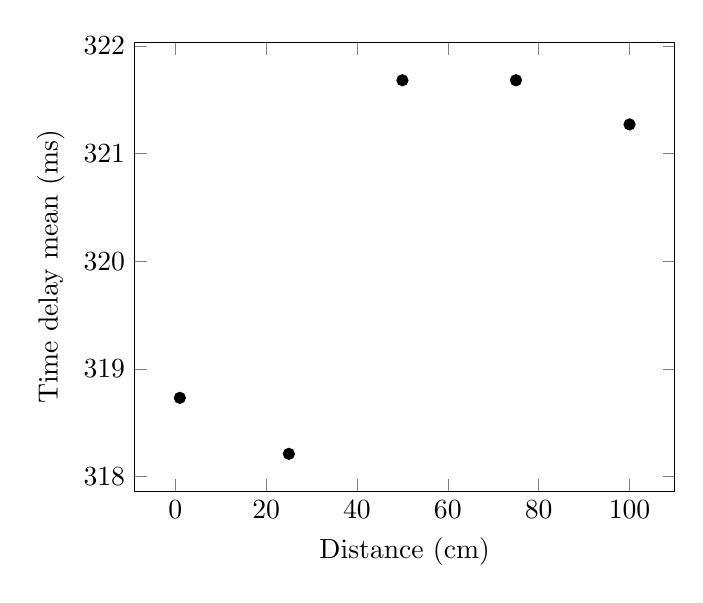
\begin{tikzpicture}
\begin{axis}[
    xlabel = {Distance (cm)},
    ylabel = {Time delay mean (ms)},
]
\addplot[
    color = black,
    fill = black,
    mark = *,
    only marks]
coordinates {
    ( 1, 318.73 )
    ( 25, 318.21 )
    ( 50, 321.68 )
    ( 75, 321.68 )
    ( 100, 321.27 )
};
\end{axis}
\end{tikzpicture}
\caption{Distance between the loudspeaker and microphone versus the time delay mean.}
\label{fig:means}
\end{figure}

From the delay mean at a distance of 1.0 cm, we can clearly see that there is a large delay that is not due to the propagation through the air.
The delay is probably caused by software latency in Matlab, hardware delays in the sound card, hardware delays in the microphone.
All these different delays add up to quite some delay, which could be variable as well.
If we take another look at the test data, and keep in mind that we have a theoretical accuracy of less than 1.0 cm, we can conclude that there are indeed other variable delays, apart from the air delay, that disrupt our measurement.\\ 
Looking at Figure \ref{fig:means} and Table \ref{tab:distances} we conclude that the distance can not be calculated accurately enough from the time delay. 


\section{Report 13}

\section{Report 14}

\section{Report 15}
To pick the optimal beacon signal, it is important to look at the autocorrelation, which is defined in equation \ref{eq:autoc}.

\begin{equation}
	R_x(n) = x(-n) * x(n)
	\label{eq:autoc}
\end{equation}

The autocorrelation must ideally be a delta peak to achieve the best matched filter results since the following approximation is used in matched filtering (Equation \ref{eq:matchedf}).

\begin{equation}
	x(-n) * y(n) = h(n) * R_x(n) \approx h(n) * \delta (n)
	\label{eq:matchedf}
\end{equation}

To define an alternative beacon signal, more criteria were introduced.
Firstly, the first and last bit of the code must be ones and the second and before-last be zeros to have a clear start and ending of the signal.
Secondly, the code must vary enough between zeros and ones, but not in a certain pattern.
This criteria, plus the original criteria of the delta-like autocorrelation resulted in the code \emph{e65a20e5}.
\\ \\
The default autocorrelation is displayed in Figure \ref{fig:default-correlation} and the alternative in Figure \ref{fig:own-correlation}.
The default autocorrelation shows a slimmer autocorrelation, but it contains high peaks around its main peak.
These peaks are way more likely to cause errors because they are almost as high as at the same location as the main peak, causing a relatively lower peak when matched filtering.
For that reason, we allowed more smaller peaks further away from the main peak to reduce the peak height near the main peak.
This way, the main peak is more prominent, likely to result in better matched filter results later on.
During system integration we can easily change this later on.
The implementation is oblivious to the changes, we only have to change one line of code.

\begin{figure}[H]
	\centering
	\setlength\figureheight{4cm}
    	\setlength\figurewidth{0.8\linewidth}
	\input{resources/default-correlation.tikz}
	\caption{Autocorrelation of the default beacon signal.}
	\label{fig:default-correlation}
\end{figure}

\begin{figure}[H]
	\centering
	\setlength\figureheight{4cm}
    	\setlength\figurewidth{0.8\linewidth}
	% This file was created by matlab2tikz v0.4.6 running on MATLAB 8.2.
% Copyright (c) 2008--2014, Nico Schlömer <nico.schloemer@gmail.com>
% All rights reserved.
% Minimal pgfplots version: 1.3
% 
% The latest updates can be retrieved from
%   http://www.mathworks.com/matlabcentral/fileexchange/22022-matlab2tikz
% where you can also make suggestions and rate matlab2tikz.
% 
\begin{tikzpicture}

\begin{axis}[%
width=\figurewidth,
height=\figureheight,
scale only axis,
xmin=0,
xmax=20000,
xlabel={Sample},
ymin=0,
ymax=500,
ylabel={Correlation}
]
\addplot [color=blue,solid,forget plot]
  table[row sep=crcr]{
1	0	\\
46	0	\\
90	0	\\
134	0	\\
178	0	\\
223	0	\\
267	0	\\
311	0	\\
355	0	\\
400	0	\\
444	0	\\
488	0	\\
532	0	\\
577	0	\\
621	0	\\
665	0	\\
709	0	\\
753	0	\\
798	0	\\
842	0	\\
886	0	\\
930	0	\\
975	0	\\
1019	0	\\
1063	0	\\
1107	0	\\
1152	0	\\
1196	0	\\
1240	0	\\
1284	0	\\
1329	0	\\
1373	0	\\
1417	0	\\
1461	0	\\
1505	0	\\
1550	0	\\
1594	0	\\
1638	0	\\
1682	0	\\
1727	0	\\
1771	0	\\
1815	0	\\
1859	0	\\
1904	0	\\
1948	0	\\
1992	0	\\
2036	0	\\
2081	0	\\
2125	0	\\
2169	0	\\
2213	0	\\
2257	0	\\
2302	0	\\
2346	0	\\
2390	0	\\
2434	0	\\
2479	0	\\
2523	0	\\
2567	0	\\
2611	0	\\
2656	0	\\
2700	0	\\
2744	0	\\
2788	0	\\
2833	0	\\
2877	0	\\
2921	0	\\
2965	0	\\
3009	0	\\
3054	0	\\
3098	0	\\
3142	0	\\
3186	0	\\
3231	0	\\
3275	0	\\
3319	0	\\
3363	0	\\
3408	0	\\
3452	0	\\
3496	0	\\
3540	0	\\
3585	0	\\
3629	0	\\
3673	0	\\
3717	0	\\
3761	0	\\
3806	0	\\
3850	0	\\
3894	0	\\
3938	0	\\
3983	0	\\
4027	0	\\
4071	0	\\
4115	0	\\
4160	0	\\
4204	0	\\
4248	0	\\
4292	0	\\
4337	0	\\
4381	0	\\
4425	0	\\
4469	0	\\
4513	0	\\
4558	0	\\
4602	0	\\
4646	0	\\
4690	0	\\
4735	0	\\
4779	0	\\
4823	0	\\
4867	0	\\
4912	0	\\
4956	0	\\
5000	0	\\
5044	0	\\
5089	0	\\
5133	0	\\
5177	0	\\
5221	0	\\
5265	0	\\
5310	0	\\
5354	0	\\
5398	0	\\
5442	0	\\
5487	0	\\
5531	0	\\
5575	0	\\
5619	0	\\
5664	0	\\
5708	0	\\
5752	0	\\
5796	0	\\
5841	0	\\
5885	0	\\
5929	0	\\
5973	0	\\
6017	0	\\
6062	0	\\
6106	0	\\
6150	0	\\
6194	0	\\
6239	0	\\
6283	0	\\
6327	0	\\
6371	0	\\
6416	0	\\
6460	0	\\
6504	0	\\
6548	0	\\
6593	0	\\
6637	0	\\
6681	0	\\
6725	0	\\
6769	0	\\
6814	0	\\
6858	0	\\
6902	0	\\
6946	0	\\
6991	0	\\
7035	0	\\
7079	0	\\
7123	0	\\
7168	0	\\
7212	0	\\
7256	0	\\
7300	0	\\
7345	0	\\
7389	0	\\
7433	0	\\
7477	0	\\
7521	0	\\
7566	0	\\
7610	0	\\
7654	0	\\
7698	0	\\
7743	0	\\
7787	0	\\
7831	0	\\
7875	0	\\
7920	0	\\
7964	0	\\
8008	0	\\
8052	0	\\
8097	0	\\
8141	0	\\
8185	0	\\
8229	0	\\
8273	0	\\
8318	0	\\
8362	0	\\
8406	0	\\
8450	0	\\
8495	0	\\
8539	0	\\
8583	0	\\
8627	0	\\
8672	0	\\
8716	0	\\
8760	0	\\
8804	0	\\
8849	0	\\
8893	0	\\
8937	0	\\
8981	0	\\
9005	30	\\
9043	60	\\
9055	8	\\
9079	7	\\
9110	70	\\
9144	118	\\
9156	22	\\
9158	87	\\
9194	10	\\
9204	19	\\
9216	125	\\
9269	110	\\
9290	19	\\
9295	16	\\
9312	92	\\
9343	33	\\
9360	160	\\
9379	139	\\
9415	22	\\
9444	22	\\
9466	143	\\
9468	37	\\
9499	190	\\
9540	35	\\
9552	155	\\
9564	37	\\
9600	475	\\
9636	37	\\
9648	155	\\
9660	35	\\
9701	190	\\
9732	37	\\
9734	143	\\
9756	22	\\
9785	22	\\
9821	139	\\
9840	160	\\
9866	30	\\
9888	92	\\
9905	16	\\
9910	19	\\
9926	110	\\
9984	125	\\
9996	19	\\
10006	10	\\
10042	87	\\
10044	22	\\
10056	118	\\
10090	70	\\
10116	7	\\
10140	8	\\
10157	60	\\
10195	30	\\
10214	0	\\
10220	0	\\
10264	0	\\
10308	0	\\
10352	0	\\
10397	0	\\
10441	0	\\
10485	0	\\
10529	0	\\
10574	0	\\
10618	0	\\
10662	0	\\
10706	0	\\
10751	0	\\
10795	0	\\
10839	0	\\
10883	0	\\
10928	0	\\
10972	0	\\
11016	0	\\
11060	0	\\
11104	0	\\
11149	0	\\
11193	0	\\
11237	0	\\
11281	0	\\
11326	0	\\
11370	0	\\
11414	0	\\
11458	0	\\
11503	0	\\
11547	0	\\
11591	0	\\
11635	0	\\
11680	0	\\
11724	0	\\
11768	0	\\
11812	0	\\
11856	0	\\
11901	0	\\
11945	0	\\
11989	0	\\
12033	0	\\
12078	0	\\
12122	0	\\
12166	0	\\
12210	0	\\
12255	0	\\
12299	0	\\
12343	0	\\
12387	0	\\
12432	0	\\
12476	0	\\
12520	0	\\
12564	0	\\
12608	0	\\
12653	0	\\
12697	0	\\
12741	0	\\
12785	0	\\
12830	0	\\
12874	0	\\
12918	0	\\
12962	0	\\
13007	0	\\
13051	0	\\
13095	0	\\
13139	0	\\
13184	0	\\
13228	0	\\
13272	0	\\
13316	0	\\
13360	0	\\
13405	0	\\
13449	0	\\
13493	0	\\
13537	0	\\
13582	0	\\
13626	0	\\
13670	0	\\
13714	0	\\
13759	0	\\
13803	0	\\
13847	0	\\
13891	0	\\
13936	0	\\
13980	0	\\
14024	0	\\
14068	0	\\
14112	0	\\
14157	0	\\
14201	0	\\
14245	0	\\
14289	0	\\
14334	0	\\
14378	0	\\
14422	0	\\
14466	0	\\
14511	0	\\
14555	0	\\
14599	0	\\
14643	0	\\
14688	0	\\
14732	0	\\
14776	0	\\
14820	0	\\
14864	0	\\
14909	0	\\
14953	0	\\
14997	0	\\
15041	0	\\
15086	0	\\
15130	0	\\
15174	0	\\
15218	0	\\
15263	0	\\
15307	0	\\
15351	0	\\
15395	0	\\
15440	0	\\
15484	0	\\
15528	0	\\
15572	0	\\
15616	0	\\
15661	0	\\
15705	0	\\
15749	0	\\
15793	0	\\
15838	0	\\
15882	0	\\
15926	0	\\
15970	0	\\
16015	0	\\
16059	0	\\
16103	0	\\
16147	0	\\
16192	0	\\
16236	0	\\
16280	0	\\
16324	0	\\
16368	0	\\
16413	0	\\
16457	0	\\
16501	0	\\
16545	0	\\
16590	0	\\
16634	0	\\
16678	0	\\
16722	0	\\
16767	0	\\
16811	0	\\
16855	0	\\
16899	0	\\
16944	0	\\
16988	0	\\
17032	0	\\
17076	0	\\
17120	0	\\
17165	0	\\
17209	0	\\
17253	0	\\
17297	0	\\
17342	0	\\
17386	0	\\
17430	0	\\
17474	0	\\
17519	0	\\
17563	0	\\
17607	0	\\
17651	0	\\
17696	0	\\
17740	0	\\
17784	0	\\
17828	0	\\
17872	0	\\
17917	0	\\
17961	0	\\
18005	0	\\
18049	0	\\
18094	0	\\
18138	0	\\
18182	0	\\
18226	0	\\
18271	0	\\
18315	0	\\
18359	0	\\
18403	0	\\
18448	0	\\
18492	0	\\
18536	0	\\
18580	0	\\
18624	0	\\
18669	0	\\
18713	0	\\
18757	0	\\
18801	0	\\
18846	0	\\
18890	0	\\
18934	0	\\
18978	0	\\
19023	0	\\
19067	0	\\
19111	0	\\
19199	0	\\
};
\end{axis}
\end{tikzpicture}%
	\caption{Autocorrelation of the alternative beacon signal.}
	\label{fig:own-correlation}
\end{figure}


\end{document} 